% !Mode:: "Tex:UTF-8"

En este capítulo vamos a conocer los dos tipos de variables aleatorias más importantes de la Estadística: las binomiales, de tipo discreto, y las normales, de tipo continuo. Además, veremos la relación que existe entre ambos tipos de variables, a través (de una primera versión) del  Teorema Central del Límite. Ese teorema es, sin duda, un resultado matemático muy profundo. Pero, por sus consecuencias prácticas, puede considerarse además como una de las leyes fundamentales de la naturaleza. Verdaderamente fundamental, al mismo nivel de partes tan esenciales de nuestra visión del mundo, como la estructura atómica, las leyes de Newton, la posición de la Tierra en el universo, la estructura celular de los seres vivos o la evolución de la especies.  Si no ha llegado al mismo nivel de popularización que esos otros resultados científicos, se debe seguramente a la barrera que supone el formalismo matemático. Pero creemos que este teorema es uno de los grandes logros intelectuales de la humanidad. Así que rogamos del lector una lectura atenta de este capítulo. Tal vez nuestras explicaciones no lo merezcan, pero las ideas que tratamos de explicar sin duda lo merecen. La comprensión de los contenidos de este y los dos próximos capítulos no sólo supone un punto de inflexión en el estudio de la Estadística, sino que marca un hito en el bagaje profesional de cualquier científico.


\section{Experimentos de Bernouilli y la Distribución Binomial.}
\label{cap05:sec:ExperimentosBernouilliDistribucionBinomial}


\subsection{Experimentos de Bernouilli.}
\label{cap05:subsec:ExperimentosBernouilli}

En muchas situaciones, el resultado de un experimento sólo admite dos resultados posibles. Son las típicas situaciones de {\em cara o cruz, ``sí o no'', acierto o fallo, ganar o perder}.
Por ejemplo:
    \begin{enumerate}
            \item Cuando lanzamos una moneda, y apostamos a que va a salir cara, entonces sólo podemos ganar la apuesta o perderla.
            \item Y si lanzamos un dado, y apostamos a que va a salir un seis, entonces sólo podemos ganar la apuesta o perderla.
            \item Al hacer pruebas diagnósticas en Medicina, nos interesa la respuesta a preguntas como:``¿El paciente es hipertenso, sí o no?''
            \item Y de forma parecida, en un proceso de fabricación industrial queremos saber si una pieza es o no defectuosa.
    \end{enumerate}
En ambas ocasiones sólo hay dos resultados posibles. La diferencia entre ellas es, naturalmente,  que la probabilidad de éxito o fracaso no es la misma. Al lanzar la moneda, la probabilidad de ganar la apuesta es $1/2$, mientras que en el caso del dado es $1/6$. Vamos a introducir la terminología que usaremos para describir este tipo de situaciones:
    \begin{center}
    \fcolorbox{black}{Gris025}{
    \begin{minipage}{13cm}
        \begin{center}
        %%%%%%%%%%%%%%%%%%%%%%%%%%%%%%%%%%%%%%%
        {\bf  Experimento de Bernouilli}\label{cap05:def:ExperimentoBernouilli}
        \end{center}
        \index{experimento de Bernouilli}
        %%%%%%%%%%%%%%%%%%%%%%%%%%%%%%%%%%%%%%%
        Un {\sf experimento de Bernouilli} es un experimento aleatorio que sólo tiene dos resultados posibles, que llamamos (arbitrariamente) {\sf éxito}\index{\'exito (experimento de Bernouilli)} y {\sf fracaso}\index{fracaso (experimento de Bernouilli)}. La {\sf probabilidad de éxito} se representa siempre con la letra $p$, mientras que la probabilidad de fracaso se representa con la letra $q$. Naturalmente, se tiene que cumplir que
        \[q=1-p.\]
        Nos referiremos a esto como a un experimento Bernouilli($p$).
        %%%%%%%%%%%%%%%%%%%%%%%%%%%%%%%%%%%%%%%
    \end{minipage}}
    \end{center}
Por ejemplo, en el caso de la moneda es $p=q=\frac{1}{2}$ (a menos, naturalmente, que la moneda esté trucada). Y en el caso del dado es $p=\frac{1}{6}$, mientras $q=\frac{5}{6}$.

Para describir el resultado de un experimento de este tipo, utilizamos un tipo especial de variables aleatorias. Una variable aleatoria $X$ es de tipo {\em Bernouilli$(p)$}\index{Bernouilli$(p)$, variable aleatoria}
si sólo puede tomar dos valores. Puesto que una variable aleatoria tiene que producir resultados numéricos, arbitrariamente, se asignan los valores
\[X(\text{éxito})= 1\qquad\qquad X(\text{fracaso})= 0,\]
con probabilidades $p$ y $q=1-p$. En resumen, estas variables tienen la tabla (o función de densidad) más sencilla posible, que puede verse  en la Tabla \ref{cap05:tabla:FuncionDensidadVariableBernouilli}.
    \begin{table}[hp]
    \begin{center}{\bf
    \begin{tabular}[t]{|c|c|c|}
        \hline
        \rule{0cm}{0.5cm}{\em Valor de $X$:}&1&0\\
        \hline
        \rule{0cm}{0.7cm}{\em Probabilidad de ese valor:}&{\em p}&{\em q}\\
        \hline
    \end{tabular}}
    \end{center}
    \label{cap05:tabla:FuncionDensidadVariableBernouilli}
    \caption{Tabla (función de densidad) para una variable de tipo Bernouilli$(p)$}
    \end{table}

\noindent En notación funcional, siendo $f_X(x)$ la función de densidad de $X$,  puedes comprobar que la Tabla \ref{cap05:tabla:FuncionDensidadVariableBernouilli} es equivalente a decir que:
\begin{equation}
\label{cap05:ecu:FuncionDensidadVariableBernouilli}
f_X(x)=p^{x}\cdot q^{1-x}.
\end{equation}
Recuerda que $X$ sólo toma los valores $0$ y $1$, y sustituye $x$ por $0$ y por $1$ en $f_X(x)$ para ver como funciona esto.

Con una función de densidad tan sencilla, es muy fácil también calcular la media y la varianza de una variable de tipo {\em Bernouilli$(p)$}. Para la media tenemos:
    \begin{equation}\label{cap05:ecu:MediaVariableBernouilli}
    \mu=E(X)=1\cdot p+0\cdot q=p.
    \end{equation}
Y para la varianza:
    \begin{equation}\label{cap05:ecu:VarianzaVariableBernouilli}
    \begin{array}{rl}
    \sigma^2& =\operatorname{Var}(X)=(1-\mu)^2\cdot p+(0-\mu)^2\cdot q\\
     &=(1-p)^2\cdot p+(0-p)^2\cdot q=q^2p+p^2q=pq\cdot(p+q)=pq.
    \end{array}
    \end{equation}
Las variables de tipo Bernouilli son muy importantes, porque los usamos como bloques básicos para construir otras situaciones más complejas. En particular, son las piezas básicas para construir la Distribución Binomial.

\subsection{Variable aleatoria binomial.}
\label{cap05:subsec:VariableAleatoriaBinomial}

Supongamos que tenemos un experimento de Bernouilli, con sus dos resultados posibles, éxito y fracaso, con probabilidades $p$ y $q$ respectivamente. Pero ahora {\em vamos a repetirlo una cierta cantidad de veces}. Y vamos a llamar $n$ al número de veces que lo repetimos. ¿Qué probabilidad hay de obtener exactamente $k$ éxitos en esos $n$ experimentos?

Para fijar ideas, el experimento de Bernouilli puede ser lanzar un dado, y vamos a suponer que lo lanzamos $n=5$ veces. ¿Cuál es la probabilidad de sacar {\em exactamente} $k=2$ seises en esos 5 lanzamientos? Antes de seguir adelante, recomendamos al lector que repase el Ejemplo \ref{cap03:ejem:probabilidadLanzamientoMonedas} (pág. \pageref{cap03:ejem:probabilidadLanzamientoMonedas}), en el que se planteaba una pregunta muy parecida, pero en aquel caso usando monedas sin trucar. La diferencia, por tanto, es que aquí, con el dado, nos planteamos un problema más general, porque las probabilidades de éxito $p=1/6$ y de fracaso $q=5/6$ son distintas, mientras que en las monedas es $p=q=1/2$. Además, también podemos ver que es una pregunta muy relacionada con los juegos del caballero De Mere. (De hecho, para obtener la respuesta al primer juego de De Mere, lo que hicimos fue calcular la probabilidad del suceso contrario: obtener exactamente {\em ningún} seis en cuatro tiradas de un dado). En el siguiente ejemplo vamos a obtener la respuesta y, como consecuencia, descubriremos la fórmula general para la Distribución Binomial. Esa distribución juega un papel tan importante en todo lo que sigue, que creemos que es fundamental entender bien este ejemplo. Por esa razón, vamos a darte dos versiones del ejemplo, con la esperanza de que, de una u otra manera, entiendas el resultado final. La situación ideal es que entiendas las dos, y llegues a ver la relación entre los dos enfoques de un mismo problema. Pero lo que es irrenunciable es que entiendas la fórmula que vamos a obtener para el resultado del problema.

\begin{Ejemplo}{\bf (Binomial, primera versión)}
\label{ejem:BinomialDosSeisesCuatroTiradas}
    El conjunto de respuestas posibles (espacio muestral) tiene $6^5$ respuestas posibles (y equiprobables). Hemos usado muchas veces el ejemplo del lanzamiento de dos dados, con $36=6^2$ resultados posibles, así que no es una sorpresa que aquí, al lanzar cinco veces, tengamos $6^5$ resultados posibles. Y si lo quieres ver desde un punto de vista combinatorio, se trat del número de variaciones con repetición de seis elementos, tomados de cinco en cinco (ver la Ecuación \ref{cap03:ecu:VariacionesConRepeticion}, pág. \pageref{cap03:ecu:VariacionesConRepeticion}).

    ¿En cuántas de esas respuestas posibles se obtienen exactamente dos seises? (Dicho de otro modo ¿cuántas ``favorables'' hay?) Como hicimos en el caso de una moneda, podemos representar los resultados de esas cinco tiradas usando un casillero con cinco casillas.
    \begin{center}
    \begin{tabular}{|c|c|c|c|c|}
    \hline
    \rule{0cm}{0.5cm}\rule{0.3cm}{0cm}&\rule{0.3cm}{0cm}&\rule{0.3cm}{0cm} &\rule{0.3cm}{0cm}&\rule{0.3cm}{0cm}\\
    \hline
    \end{tabular}
    \end{center}
    Los dos seises se pueden haber obtenido en la primera y segunda casillas, o en la primera y la tercera, etcétera. Marcamos con un $6$ las casillas en las que se han obtenido los seises. Las tres casillas restantes contienen números que no son seis. Los posibles resultados están en la Tabla \ref{cap05:tabla:FormasColocarDosSeisesCincoCasillas}.
        \begin{table}[ht]
        \begin{center}
        {
        \begin{tabular}{|c|c|c|c|c|}
        \hline
         \mbox{ \bf 6}&\mbox{ \bf 6}& & & \\
        \hline
         \mbox{ \bf 6}&& \mbox{ \bf 6}& & \\
        \hline
         \mbox{ \bf 6}&& &\mbox{ \bf 6} & \\
        \hline
         \mbox{ \bf 6}&& & &\mbox{ \bf 6} \\
        \hline
         &\mbox{ \bf 6}& \mbox{ \bf 6}& & \\
        \hline
         &\mbox{ \bf 6}& &\mbox{ \bf 6} & \\
        \hline
         &\mbox{ \bf 6}& & & \mbox{ \bf 6}\\
        \hline
         && \mbox{ \bf 6}&\mbox{ \bf 6} & \\
         \hline
         && \mbox{ \bf 6}& & \mbox{ \bf 6} \\
         \hline
         &&& \mbox{ \bf 6}& \mbox{ \bf 6} \\
         \hline
        \end{tabular}
        }
        \caption{Formas distintas de colocar dos seises en cinco casillas}\label{cap05:tabla:FormasColocarDosSeisesCincoCasillas}
        \end{center}
        \end{table}
    Hay, como puede verse, diez posibilidades. Una forma de obtener este número, sin tener que construir a mano todas las posibilidades, es observando que lo que hacemos es elegir dos de entre cinco casillas, sin que nos importe el orden. Ese es un problema de combinaciones, y sabemos que hay:
         \[\binom{5}{2}=\dfrac{5\cdot 4}{2}=10\]
    formas distintas de hacer esa elección, de dos casillas entre cinco.

    Una vez que hemos decidido donde colocar los dos seises, todavía tenemos que pensar en los resultados de los restantes tres lanzamientos. Si, por ejemplo, hemos obtenido los dos seises en el primer y segundo lanzamiento, tendremos las $5^3=125$ posibilidades que se ilustran en la Tabla \ref{cap05:tabla:RellenandoTresCasillasRestantes}.
        \begin{table}[ht]
        \begin{center}
        \[
        \left.\begin{array}{|c|c|c|c|c|}
        \hline
         \rule{0cm}{0.5cm}\mbox{\large\bf 6}&\mbox{\large\bf 6}&\mbox{\large\bf 1}&\mbox{\large\bf 1}&\mbox{\large\bf 1}\\
        \hline
        \rule{0cm}{0.5cm}\mbox{\large\bf 6}&\mbox{\large\bf 6}&\mbox{\large\bf 1}&\mbox{\large\bf 1}&\mbox{\large\bf 2}\\
        \hline
        \rule{0cm}{0.5cm}\vdots&\vdots&\vdots&\vdots&\vdots\\
        \hline
        \rule{0cm}{0.5cm}\mbox{\large\bf 6}&\mbox{\large\bf 6}&\mbox{\large\bf 1}&\mbox{\large\bf 1}&\mbox{\large\bf 5}\\
        \hline
        \rule{0cm}{0.5cm}\mbox{\large\bf 6}&\mbox{\large\bf 6}&\mbox{\large\bf 2}&\mbox{\large\bf 1}&\mbox{\large\bf 1}\\
        \hline
        \rule{0cm}{0.5cm}\mbox{\large\bf 6}&\mbox{\large\bf 6}&\mbox{\large\bf 2}&\mbox{\large\bf 1}&\mbox{\large\bf 2}\\
        \hline
        \rule{0cm}{0.5cm}\vdots&\vdots&\vdots&\vdots&\vdots\\
        \hline
        \rule{0cm}{0.5cm}\mbox{\large\bf 6}&\mbox{\large\bf 6}&\mbox{\large\bf 5}&\mbox{\large\bf 5}&\mbox{\large\bf 5}\\
        \hline
         \end{array}\quad\right\}\,\,5^3=125\mbox{ posibilidades}
         \]
        \caption{Rellenando las tres casillas restantes, tras colocar dos seises en una posición concreta}\label{cap05:tabla:RellenandoTresCasillasRestantes}
        \end{center}
        \end{table}
    De nuevo, podemos obtener este resultado usando la Combinatoria: una vez que sabemos cuáles son las tres casillas que han quedado vacantes, tras colocar dos seises, tenemos que situar allí tres números, elegidos del uno al cinco, que pueden repetirse y el orden es importante. Esta es la descripción de un problema de variaciones con repetición, de cinco elementos tomados de tres en tres, y de nuevo, como al contar los casos posibles, la fórmula adecuada es la Ecuación \ref{cap03:ecu:VariacionesConRepeticion} (pág. \pageref{cap03:ecu:VariacionesConRepeticion}).

    Hay que subrayar que ese número de posibilidades, 125, es el mismo sea cual sea la posición en la que hayamos colocado los dos seises. Y por lo tanto, para cada una de las 10 formas de colocar los seises, tenemos 125 formas de rellenar las tres casillas restantes. Por lo tanto, el número de casos favorables es:
        \[\small\mbox{(formas de colocar los dos seises)}\cdot\mbox{(formas de rellenar las tres  restantes)}=\binom{5}{2} \cdot 5^3,\]
    y la probabilidad que queríamos calcular es:
         \[\dfrac{\displaystyle\binom{5}{2}5^3}{6^5}=\dfrac{625}{3888}\approx 0.1608\]

     Vamos a intentar generalizar a partir de aquí: ¿y si hubiéramos lanzado los dados nueve veces, y de nuevo nos preguntáramos por la probabilidad de obtener dos seises? Sería:
     \[\dfrac{\displaystyle\binom{9}{2}5^{9-2}}{6^9},\]
     donde el $9-2=7$ corresponde a las siete casillas que tenemos que rellenar con números distintos de $6$. Es interesante recordar que lo que hacemos, en este caso, es repetir $n=9$ veces un experimento de Bernouilli que tiene $p=\dfrac{1}{6}$ como probabilidad de éxito y $q=\dfrac{5}{6}$ como probabilidad de fracaso. Y lo que nos preguntamos es la probabilidad de obtener $k=2$ éxitos (y por lo tanto, claro, $9-2$ fracasos). Teniendo esto en cuenta, podemos escribir los resultado que acabamos de obtener de una forma más útil, que lo relaciona con los parámetros del experimento de Bernouilli subyacente. Separamos los nueve seises del denominador en dos grupos: dos corresponden a los éxitos, y siete a los fracasos. Obtenemos:
     \[\dfrac{\displaystyle\binom{9}{2}5^{9-2}}{6^9}=
     \mbox{\large $ \displaystyle\binom{9}{2}$}\cdot\left(\dfrac{1}{6}\right)^2\cdot\left(\dfrac{5}{6}\right)^{9-2}=
     \binom{n}{k}\cdot p^k\cdot q^{n-k}.
     \]
     ¿Y en el ejemplo original, con cinco lanzamientos, funciona también esto? Teníamos
     \[\dfrac{\displaystyle\binom{5}{2}5^3}{6^5},\]
     así que de nuevo separamos los cinco seises del denominador en dos grupos: dos corresponden a los éxitos, y tres a los fracasos. Obtenemos, otra vez:
     \[\dfrac{\displaystyle\binom{5}{2}5^{5-2}}{6^5}=
     \mbox{\large $ \displaystyle\binom{5}{2}$}\cdot\left(\dfrac{1}{6}\right)^2\cdot\left(\dfrac{5}{6}\right)^{5-2}=
     \binom{n}{k}\cdot p^k\cdot q^{n-k}.
     \]
     Así que parece que hemos dado con la respuesta general.
     \quad\qed
\end{Ejemplo}

\noindent Y ahora, veamos la segunda versión:

\begin{Ejemplo}{\bf (Binomial, segunda versión)}\label{ejem:BinomialDosSeisesCuatroTiradasMarcos} El enfoque ahora
resulta algo más teórico, y enlaza directamente con el lenguaje de la probabilidad estudiado en el capítulo 3.
Queremos determinar la siguiente probabilidad:
            	\[P(\text{Sacar $2$ veces seis, al lanzar $5$ veces un dado})\]
            %El conjunto de respuestas posibles (espacio muestral) tiene $6^5$ respuestas posibles (y equiprobables).
            En primera instancia nos preguntamos ¿de cuántas formas se obtienen exactamente $2$ seises en $5$ lanzamientos? %(Dicho de otro modo ¿cuántas ``favorables'' hay?)
             Podemos representar los resultados de esas $5$ tiradas usando un casillero con $5$  casillas.
            \begin{center}
            \begin{tabular}{|c|c|c|c|c|}
            \hline
             \rule{0cm}{0.5cm}\rule{0.3cm}{0cm}&\rule{0.3cm}{0cm}&\rule{0.3cm}{0cm} &\rule{0.3cm}{0cm}
             &\rule{0.3cm}{0cm}\\
             \hline
             \end{tabular}
             \end{center}
             Los $2$ seises se pueden haber obtenido en la primera y segunda casillas, o en la primera y la tercera, etcétera.
    En la Tabla \ref{cap05:tabla:FormasSacarDosVecesSeisCincoTiradasDado} marcamos con un $6$ las casillas en las que se han obtenido los seises. Adem\'as, pondremos nombre a los eventos; en la primera columna: con $A_1$ nos referimos al caso en el que los seises están en las casillas 1 y 2, y así sucesivamente. Y  ''traduciremos'' los eventos a \'exitos (E) y fracasos (F), que tienen probabilidad $p=1/6$ y $q=1-p=5/6$, respectivamente:
    \begin{table}[htbp]
        \begin{center}
          \begin{tabular}{|c|c|c|c|c|c|}
            \hline
            $A_1$ &  \rule{0cm}{0.5cm}\mbox{\large\bf 6}&\mbox{\large\bf 6}& & & \\
            \hline
            $A_2$ &  \rule{0cm}{0.5cm}\mbox{\large\bf 6}&& \mbox{\large\bf 6}& & \\
            \hline
            $A_3$ &  \rule{0cm}{0.5cm}\mbox{\large\bf 6}&& &\mbox{\large\bf 6} & \\
            \hline
            $A_4$ &  \rule{0cm}{0.5cm}\mbox{\large\bf 6}&& & &\mbox{\large\bf 6} \\
            \hline
            $A_5$ &  \rule{0cm}{0.5cm}&\mbox{\large\bf 6}& \mbox{\large\bf 6}& & \\
            \hline
            $A_6$ &  \rule{0cm}{0.5cm}&\mbox{\large\bf 6}& &\mbox{\large\bf 6} & \\
            \hline
            $A_7$ &  \rule{0cm}{0.5cm}&\mbox{\large\bf 6}& & & \mbox{\large\bf 6}\\
            \hline
            $A_8$ &  \rule{0cm}{0.5cm}&& \mbox{\large\bf 6}&\mbox{\large\bf 6} & \\
             \hline
            $A_9$ &  \rule{0cm}{0.5cm}&& \mbox{\large\bf 6}& & \mbox{\large\bf 6} \\
             \hline
            $A_{10}$ &  \rule{0cm}{0.5cm}&&& \mbox{\large\bf 6}& \mbox{\large\bf 6} \\
             \hline
             \end{tabular}
             $\Leftrightarrow$
         \begin{tabular}{|c|c|c|c|c|}
            \hline
         \rule{0cm}{0.5cm}\mbox{\large\bf E}&\mbox{\large\bf E}&F & F&F \\
            \hline
             \rule{0cm}{0.5cm}\mbox{\large\bf E}&F& \mbox{\large\bf E}&F &F \\
            \hline
            \rule{0cm}{0.5cm}\mbox{\large\bf E}&F&F &\mbox{\large\bf E} & F\\
            \hline
           \rule{0cm}{0.5cm}\mbox{\large\bf E}&F&F & F&\mbox{\large\bf E} \\
            \hline
             \rule{0cm}{0.5cm}F&\mbox{\large\bf E}& \mbox{\large\bf E}&F & F\\
            \hline
            \rule{0cm}{0.5cm}F&\mbox{\large\bf E}&F &\mbox{\large\bf E} & F\\
            \hline
            \rule{0cm}{0.5cm}F&\mbox{\large\bf E}&F &F & \mbox{\large\bf E}\\
            \hline
            \rule{0cm}{0.5cm}F&F& \mbox{\large\bf E}&\mbox{\large\bf E} &F \\
             \hline
             \rule{0cm}{0.5cm}F&F& \mbox{\large\bf E}& F & \mbox{\large\bf E} \\
             \hline
             \rule{0cm}{0.5cm}F&F&F& \mbox{\large\bf E}& \mbox{\large\bf E} \\
             \hline
             \end{tabular}
                    $\Leftrightarrow$
         \begin{tabular}{|c|c|c|c|c|}
            \hline
             \rule{0cm}{0.5cm}\mbox{\large\bf p}&\mbox{\large\bf p}&q & q&q \\
            \hline
             \rule{0cm}{0.5cm}\mbox{\large\bf p}&q& \mbox{\large\bf p}&q &q \\
            \hline
             \rule{0cm}{0.5cm}\mbox{\large\bf p}&q&q &\mbox{\large\bf p} & q\\
            \hline
             \rule{0cm}{0.5cm}\mbox{\large\bf p}&q&q & q&\mbox{\large\bf p} \\
            \hline
             \rule{0cm}{0.5cm}q&\mbox{\large\bf p}& \mbox{\large\bf p}&q & q\\
            \hline
             \rule{0cm}{0.5cm}q&\mbox{\large\bf p}&q &\mbox{\large\bf p} & q\\
            \hline
             \rule{0cm}{0.5cm}q&\mbox{\large\bf p}&q &q & \mbox{\large\bf p}\\
            \hline
             \rule{0cm}{0.5cm}q&q& \mbox{\large\bf p}&\mbox{\large\bf p} &q \\
             \hline
             \rule{0cm}{0.5cm}q&q& \mbox{\large\bf p}& q & \mbox{\large\bf p} \\
             \hline
              \rule{0cm}{0.5cm}q&q&q& \mbox{\large\bf p}& \mbox{\large\bf p} \\
             \hline
             \end{tabular}
        \caption{Formas de sacar $2$ veces seis, al lanzar $5$ veces un dado}\label{cap05:tabla:FormasSacarDosVecesSeisCincoTiradasDado}
        \end{center}
        \end{table}

         Hay diez posibilidades, pero vamos a intentar no contar con los dedos (eso est\'a ah\'i s\'olo para apoyar nuestra intuici\'on, pero saldremos ganando si somos capaces de abstraer lo importante). Ahora podemos escribir
          	\[P(\text{Sacar $2$ veces seis al lanzar $5$ veces un dado})=\]
          	\[=P(\text{Suceda $A_1$, o bien suceda $A_2$, \dots, o bien suceda $A_{10}$})
          	\]
         Para no complicarnos tanto la vida de entrada, vamos a considerar la probabilidad de que se de, o bien $A_1$, o bien $A_2$. Esto, en lenguaje conjuntista, es
         \[P(\text{Suceda o bien $A_1$, o bien suceda $A_2$)}=P(A_1\cup A_2).\]
         Aparece la probabilidad de la uni\'on de dos eventos. Esto debería traerte a la cabeza
         lo explicado en la Secci\'on \ref{Cap03:def:DefinicionProbabilidad}, en la que hemos visto         la forma de operar con este tipo de problemas; en concreto (Ecuación \ref{cap03:ecu:ProbabilidadUnionDosSucesosCasoGeneral}, pág. \pageref{cap03:ecu:ProbabilidadUnionDosSucesosCasoGeneral})
		\[P(A_1\cup A_2)=P(A_1)+P(A_2)-P(A_1\cap A_2).\]
    Además, es importante el hecho de que los eventos $A_1$ y $A_2$ son incompatibles: efectivamente, si tiene que haber 2 seises, estos no pueden estar en las casillas $1$ y $2$ (por $A_1$), y a la vez en las casillas $2$ y $3$ (por $A_2$), porque habría 3 seises. Esto nos dice (ver la segunda de las Propiedades Fundamentales de la Probabilidad, pág. \pageref{cap03:def:PropiedadesFundamentalesFuncionProbabilidad}) que (puesto que $P(A_1\cap A_2)=0$), se cumple:
%         Sabemos que lo que obtengamos en una serie de lanzamientos (de hecho, en cada lanzamiento)
%         es independiente de lo que obtenemos en otra. Gracias a una de las propiedades fundamentales de la funci\'on  de probabilidad, cuando los eventos son incompatibles
         %\pendiente{En esta parte creo que quieres decir incompatibles, no independientes} YA ESTÁ ARREGLADO\\
%         (ver la segunda de las Propiedades Fundamentales de la Probabilidad, pág. \pageref{cap03:def:PropiedadesFundamentalesFuncionProbabilidad}) se cumple que
         \[P(A_1\cup A_2)=P(A_1)+P(A_2).\]
         A poco que lo pensemos\footnote{Podemos empezar con $A_1$, $A_2$ y $A_3$.
         Hemos acordado que son incompatibles, de modo que $A_1$ y $B=A_2\cup A_3$ tambi\'en lo son.
         As\'i pues, $P(A_1\cup B)= P(A_1)+P( B)$, y ahora podemos aplicar de nuevo la propiedad de los sucesos incompatibles, para desomponer $P(B)$ en la suma de $P(A_2)$ y $P(A_3$.} nos convenceremos de que
         \[P(\text{Suceda $A_1$, o bien suceda $A_2$, \dots, o bien suceda
         $A_{10}$})=\]
	\[P(A_1\cup A_2 \cup \cdots \cup A_{10}) =P(A_1)+P(A_2)+\cdots+P(A_{10}).\\
                   	\]
          Estamos más cerca. Habremos respondido a la pregunta inicial si somos capaces de calcular la probabilidad de cada uno de los sumandos.

        Vamos a por el primero de ellos, en el que sale seis en los $2$  primeros lanzamientos (y no sale en los $3$ \'ultimos). La clave consiste en expresar el valor $P(A_1)$ (que desconocemos) en términos de cantidades conocidas. Sabemos cuánto vale la probabilidad de sacar un seis $P(E)=1/6)$ y de no sacarlo $P(F)=5/6$. Y la estrategia consiste en expresar $P(A_1)$ a partir de $P(E)$ y $P(F)$. Vamos allá. Si llamamos $E_j$ y $F_j$, respectivamente, a los sucesos ``sacar un seis'' y ``no sacar un seis''  en el lanzamiento n\'umero $j=1,2,3,4,5$, tenemos
          	\[P(A_1)=P(E_1\cap E_2 \cap F_3\cap F_4\cap F_5)\]
        De nuevo entra en juego otra propiedad probabilística: cada lanzamiento es independiente de los dem\'as y, por tanto, usando la generalización de la Regla del Producto \ref{cap03:ecu:ReglaProductoProbabilidad_N_SucesosIndependientes} (pág. \pageref{cap03:ecu:ReglaProductoProbabilidad_N_SucesosIndependientes}) al caso de $n$ sucesos independientes:
          	\[\begin{array}{rl}
          	P(E_1\cap E_2 \cap F_3\cap F_4\cap F_5)& =P(E_1)\cdot P( E_2 )\cdot P( F_3)\cdot P( F_4)
          	\cdot P( F_5) \\
          	& \\
          	& =p\cdot p \cdot q \cdot q \cdot q = p^2\cdot q^3
          	\end{array}\]
        De hecho, el c\'alculo que acabamos de hacer da el mismo resultado para cada una           	de las series de lanzamientos $A_1,\ldots,A_{10}$, es decir
          		\[P(A_i)=p^2\cdot q^3 \qquad \text{para cualquier }i=1,\cdots,10. \]
        Como hay $10$ sumandos, la respuesta r\'apida es que la probabilidad que buscamos vale
          		\[10\cdot p^2\cdot q^3=10\cdot\left( \dfrac{1}{6}\right)^2\left(\dfrac{5}{6}\right)^3. \]	
          	Est\'a claro que $10$ es el n\'umero de formas distintas en las que se obtienen $2$ seises
          	al hacer $5$ lanzamientos.
          	Esa respuesta ser\'a de utilidad si razonamos la relaci\'on entre $10$
          	y los datos del problema. Hacemos $5$ lanzamientos, que llamaremos $1,2,3,4,5$,
          	y los eventos $A_i$ 	describen en qu\'e posici\'on han salido los $2$ seises.
          	Por ejemplo, $A_1$ se corresponde con $\left\{1,2\right\}$, $A_3$ con $\left\{1,3\right\}$,
          	y as\'i sucesivamente. Y aqu\'i entran en escena las combinaciones:
          	las posiciones en las que salen los $2$ seises vienen dadas por los
          	subconjuntos de $2$ elementos (el orden no importa) del conjunto
          	 $\left\{1,2,3,4,5\right\}$, que es el conjunto 	de las posiciones.
          	De modo que ya lo tenemos,
          		\[P(\text{Sacar $2$ veces seis, al lanzar $5$ veces un dado})=
          		\binom{5}{2}\left( \dfrac{1}{6}\right)^2\left(\dfrac{5}{6}\right)^3\]
          \qed
\end{Ejemplo}
Con este ejemplo ya estamos listos para la definición:
    \begin{center}
    \fcolorbox{black}{Gris025}{
    \begin{minipage}{12cm}
        \begin{center}
        %%%%%%%%%%%%%%%%%%%%%%%%%%%%%%%%%%%%%%%
        {\bf  Variable aleatoria binomial   }
        \end{center}
        \index{variable aleatoria binomial}
        \index{binomial, variable aleatoria}
        %%%%%%%%%%%%%%%%%%%%%%%%%%%%%%%%%%%%%%%
        Una variable aleatoria discreta $X$ es de {\sf tipo binomial con parámetros $n$ y $p$}, lo que se representa con el símbolo $B(n,p)$, si $X$ representa el número de éxitos en la repetición de $n$ experimentos independientes de Bernouilli, con probabilidad $p$ de éxito en cada uno de ellos (y con $q=1-p$).\\[3mm]
        Si $X$ es una variable aleatoria binomial de tipo $B(n,p)$, la probabilidad $P(X=k)$, es decir la probabilidad de obtener $k$ éxitos viene dada por:
		\begin{equation}
        \label{cap05:ecu:DensidadBinomial}
            \displaystyle P(X=k)=\binom{n}{k}\cdot p^k\cdot q^{n-k}.
        \end{equation}
        %La función $f(k)$ es, de hecho, la {\em función de densidad} de la distribución binomial.
       \vspace{1mm}
        %%%%%%%%%%%%%%%%%%%%%%%%%%%%%%%%%%%%%%%
    \end{minipage}}
    \end{center}
Un comentario sobre esta definición, para aclarar más la relación entre las variables binomiales y las de Bernouilli: la suma de $n$ variables independientes (ver Sección \ref{cap04:sec:IndependenciaVariablesAleatoriasDiscretas}, pág. \pageref{cap04:sec:IndependenciaVariablesAleatoriasDiscretas}) $X_1,\ldots,X_n$ de tipo Bernouilli$(p)$ es una variable aleatoria binomial $X$ de tipo $B(n,p)$. En el ejemplo del dado se puede ver esto con claridad: las variables $X_1$,\ldots,$X_n$ representan cada una de las $n$ veces que lanzamos el dado, y valen $1$ si obtenemos $6$ (éxito) en ese lanzamiento, o $0$ (fracaso) si obtenemos cualquier otro número. Además, los lanzamientos son independientes entre sí. Esto es muy importante. Nos podemos encontrar, más adelante, con un experimento que tiene $n$ etapas, y en el que el resultado total es la suma de los éxitos/fracasos de cada etapa. Pero si cada etapa del experimento afecta a las siguientes, entonces no habrá independencia, y el resultado no será una binomial.
\begin{ejemplo}
\label{cap05:ejem:ProcesoNoBinomial}
    Para ver un ejemplo de uno de estos procesos, imaginemos que tenemos dos urnas: una blanca, que contiene seis bolas, numeradas del 1 al 6, y una negra, que contiene 10 bolas, cinco numeradas del 1 al 5, y otras cinco todas numeradas con un 6. Para empezar, sacamos una bola de la urna blanca. A partir de ahí, en cada paso:
      \begin{itemize}
        \item si la bola extraída es un seis, en el siguiente paso usamos la urna negra.
        \item si la bola extraída es distinta de seis, en el siguiente paso usamos la urna blanca.
        \item en cualquier caso, la bola extraída se devuelve a la urna de la que procede y esta se agita bien.
      \end{itemize}
    Siguiendo estas reglas, extraemos $n=50$ bolas, y considerando que el {\em éxito}, en cada paso, es obtener un seis, definimos
        \[X=\{\mbox{número total de seises obtenidos}\}.\]
    Los ingredientes más básicos son parecidos: hay un proceso en $n$ pasos, en cada paso hay dos posibles resultados, éxito y fracaso. Pero la hipótesis de que el resultado de cada paso es independiente de los demás, aquí es rotundamente falsa. La urna que usamos, en cada paso, la determina el resultado del paso anterior. Y la probabilidad de éxito o fracaso es distinta en cada urna.\qed
\end{ejemplo}
En los Tutoriales usaremos el ordenador para simular este proceso. Y comprobaremos que no se parece a una binomial. Pero para eso, primero tenemos que aprender más sobre la binomial, para saber distinguirla de otras situaciones.


\subsubsection*{Tabla o función de densidad de una variable binomial.}
\label{cap05:subsubsec:tablaFuncionDensidadBinomial}

Vamos a tratar de situar la Ecuación \ref{cap05:ecu:DensidadBinomial} (pág. \pageref{cap05:ecu:DensidadBinomial}) en el contexto y el lenguaje de las variables aleatorias discretas que hemos desarrollado en el Capítulo \ref{cap:Probabilidad}. Allí vimos que si una variable aleatoria discreta $X$ toma una cantidad finita de valores numéricos $x_1,x_2,x_3,\ldots,x_k$, con probabilidades $p_i=P(X=x_i)$, su función de densidad se puede representar como una tabla (ver la  Tabla \ref{cap04:tabla:tablaDensidadProbabilidadGenericaVariableAleatoriaDiscreta}, página \pageref{cap04:tabla:tablaDensidadProbabilidadGenericaVariableAleatoriaDiscreta}).
Las variables de tipo binomial son variables discretas, así que se pueden representar mediante una de estas tablas.
\begin{ejemplo}
\label{cap05:ejem:TablaDensidadBinomial}
Por ejemplo, una variable binomial $X$ de tipo $B(3,1/5)$ puede tomar los valores $0, 1, 2, 3$ (estos son los $x_1,x_2,\ldots,x_k$ en este caso) ¿Cuál sería su tabla (función) de densidad? Sería la Tabla \ref{cap04:tabla:EjemploTablaDensidadBinomial}, en la que, como se ve, cada una de las probabilidades se calcula con la fórmula general que hemos encontrado.
{\small
    \begin{table}[ht]
    \begin{center}
    \begin{tabular}[t]{|c|c|c|c|c|}
    \hline
    \rule{0cm}{0.5cm}{\em\scriptsize Valor:}&$0$&$1$&$2$&$3$\\
    \hline
    \rule{0cm}{0.7cm}{\em {\scriptsize Probabilidad:}}&
    $\binom{3}{0}\left(\frac{1}{5}\right)^0\left(\frac{4}{5}\right)^{3-0}$&
    $\binom{3}{1}\left(\frac{1}{5}\right)^1\left(\frac{4}{5}\right)^{3-1}$&
    $\binom{3}{2}\left(\frac{1}{5}\right)^2\left(\frac{4}{5}\right)^{3-2}$&
    $\binom{3}{3}\left(\frac{1}{5}\right)^3\left(\frac{4}{5}\right)^{3-3}$
    \\[3mm]
    \hline
    \end{tabular}
    \end{center}
    \caption{Tabla de densidad de probabilidad de una variable $B(3,1/5)$}
    \label{cap04:tabla:EjemploTablaDensidadBinomial}
    \end{table}
}
\end{ejemplo}
\noindent Y si, en lugar de la tabla, preferimos usar la notación funcional, podemos decir que la función de densidad de una variable binomial de tipo $B(n,p)$ viene dada por:
\begin{equation}\label{cap05:ecu:FuncionDensidadVariableBinomial}
f(k)=P(X=k)=\binom{n}{k}\cdot p^k\cdot q^{n-k}, \mbox{ para }k=0,1,\ldots,n.
\end{equation}


A la vista del Ejemplo \ref{cap05:ejem:TablaDensidadBinomial}, en el que los números son muy sencillos  $\left(n=3, p=\frac{1}{5}\right)$, debería empezar a estar claro que no nos podemos plantear el cálculo ``a mano'' de los valores $P(X=k)$ de la distribución binomial, sustituyendo en los coeficientes binomiales, etc. Es necesario, en todos salvo los casos más simples, recurrir al ordenador para obtener estos valores. Antes, cuando los ordenadores no eran tan accesibles, se usaban tablas impresas para distintos valores de $n, p$ y $k$, que aún puedes encontrar en la parte final de muchos libros de Estadística. Nosotros vamos a aprender, en el Tutorial05, a utilizar para esto el ordenador, o cualquier dispositivo capaz de navegar por Internet.

\subsection*{Media y desviación típica de una variable aleatoria binomial.}

Como hemos dicho, una variable aleatoria binomial $X$ de tipo $B(n,p)$ se puede considerar como la suma de $n$ variables $X_1,\ldots,X_n$ de tipo Bernouilli$(p)$, que además son independientes. ¿Y de qué sirve saber esto? Podemos ver una primera muestra de la utilidad de este tipo de resultados, para calcular la media y la varianza de una variable binomial. Antes de hacerlo, vamos a considerar brevemente lo que tendríamos que hacer para calcular la media si aplicáramos directamente la definición. Tendríamos que calcular:
\[\mu=\sum_{k=0}^n k\cdot P(X=k)= \sum_{k=0}^n k\cdot\binom{n}{k}\cdot p^k\cdot q^{n-k}.\]
El resultado de la suma, planteado así, no es evidente.
\begin{ejemplo}
\label{cap05:ejem:MediaBinomialCalculoDirecto}
Por ejemplo, para un caso sencillo como el $n=3$, $p=1/5$ que hemos visto antes, tendremos que calcular:
{\small
\[0\cdot\binom{3}{0}\left(\frac{1}{5}\right)^0\left(\frac{4}{5}\right)^{3}+
1\cdot\binom{3}{1}\left(\frac{1}{5}\right)^1\left(\frac{4}{5}\right)^{2}+
2\cdot\binom{3}{2}\left(\frac{1}{5}\right)^2\left(\frac{4}{5}\right)^{1}+
3\cdot\binom{3}{3}\left(\frac{1}{5}\right)^3\left(\frac{4}{5}\right)^{3}
\]
}
\qed
\end{ejemplo}
\noindent En cambio, si pensamos en la binomial como suma de variables Bernouilli independientes, podemos
aplicar los resultados de la Sección \ref{sec:OperacionesVariablesAleatorias}, en los que aprendimos a calcular la media y la varianza de una suma de variables aleatorias independientes.
Sea $X$ una binomial $B(n,p)$ que es la suma de $n$ variables independientes $X_1,\ldots,X_n$ de tipo Bernouilli$(p)$:
\[X=X_1+\cdots+X_n\]
Recordemos (ver Ecuaciones \ref{cap05:ecu:MediaVariableBernouilli} y \ref{cap05:ecu:VarianzaVariableBernouilli}, pág. \pageref{cap05:ecu:VarianzaVariableBernouilli}) que las variables Bernouilli$(p)$ tienen media $p$ y varianza $pq$.
Entonces, por la Sección \ref{sec:OperacionesVariablesAleatorias}, tenemos, para la media:
\[\mu_X=E(X)=E(X_1)+\cdots+E(X_n)=p+\cdots+p=np,\]
y para la varianza (gracias a la independencia):
\[\sigma^2_X=\operatorname{Var}(X)=\operatorname{Var}(X_1)+\cdots+\operatorname{Var}(X_n)=pq+\cdots+pq=npq\]
En resumen:
    \begin{center}
    \fcolorbox{black}{Gris025}{
    \begin{minipage}{12cm}
        \begin{center}
        %%%%%%%%%%%%%%%%%%%%%%%%%%%%%%%%%%%%%%%
        {\bf  Media y varianza de una variable aleatoria de tipo $B(n,p)$}
        \end{center}
        \index{media de una variable binomial $B(n,p)$}
        \index{varianza de una variable binomial $B(n,p)$}
        \index{desviación típica de una variable binomial $B(n,p)$}
        %%%%%%%%%%%%%%%%%%%%%%%%%%%%%%%%%%%%%%%
           La media de una variable aleatoria discreta de tipo binomial $B(n,p)$ es
           \begin{equation}\label{cap05:ecu:MediaBinomial}
            \mu=n\cdot p
           \end{equation}
           mientras que su {\sf desviación típica}  es
           \begin{equation}\label{cap05:ecu:DesviaciontipicaBinomial}
           \sigma=\sqrt{n\cdot p\cdot q}.
           \end{equation}
        %%%%%%%%%%%%%%%%%%%%%%%%%%%%%%%%%%%%%%%
    \end{minipage}}
    \end{center}
\begin{ejemplo}
{\bf (Continuación del Ejemplo \ref{cap05:ejem:MediaBinomialCalculoDirecto}, pág. \pageref{cap05:ejem:MediaBinomialCalculoDirecto})}.
\label{cap05:ejem:MediaBinomialCalculoFormula}
En el ejemplo $B(3,1/5)$ (con $q=4/5$), se obtiene $\mu=\dfrac{3}{5}$, $\sigma=\dfrac{\sqrt{12}}{5}$.
\qed
\end{ejemplo}
Como puede verse, la descomposición de la Binomial en suma de variables Bernouilli nos ha permitido resolver de manera muy sencilla este problema, descomponiéndolo en piezas simples (una estrategia de ``divide y vencerás'').

\subsection{Un  zoológico de distribuciones binomiales.}
\label{cap05:subsec:ZooDistribucionesBinomiales}

Las distribuciones binomiales constituyen la primera familia importante de distribuciones que
encontramos en el curso. Hablamos de una familia de distribuciones porque, a medida que los
parámetros $n$ y $p$ cambian, la {\em forma} de la distribución binomial cambia. Y vamos a dedicar
esta sección a detenernos un momento a contemplar la variedad de distribuciones binomiales que
podemos obtener jugando con los valores de $n$ y $p$. En el Tutorial05 usaremos el ordenador para que puedas experimentar con las ideas de este apartado de forma dinámica, lo cual es muy recomendable.

Hablamos de la forma de la distribución binomial, y nos referimos a la forma en que se reparte, o
se {\em distribuye}, la probabilidad. Para ayudar a visualizar esa distribución de probabilidad,
vamos a utilizar gráficos muy parecidos a los gráficos de columnas que hemos visto en el Capítulo
\ref{cap:IntroduccionEstadisticaDescriptiva}. Por ejemplo, la parte (a) de la Figura
\ref{cap01:fig:ZooBinomial01} (pág. \pageref{cap01:fig:ZooBinomial01}) muestra la Binomial
$B(10,\frac{1}{2})$. Como puede verse, la figura es simétrica respecto de la media $\mu_X=n\cdot
p=5$, y tiene una forma bastante ``triangular''.  Si, manteniendo el valor de $n=10$, desplazamos
$p$ hacia valores pequeños, como $p=1/10$, se obtiene la parte (b) de la Figura
\ref{cap01:fig:ZooBinomial01}.  Como $X$ representa el número de éxitos, al hacer la probabilidad
de éxito $p$ muy pequeña, los valores de $X$ más probables serán los valores más bajos. Eso se
traduce en que el máximo de la distribución de probabilidad se desplaza hacia la izquierda, hacia
valores más pequeños de la variable $X$. De hecho, los valores a partir de $X=6$ tienen
probabilidades tan pequeñas que en la figura apenas se aprecian. Esos valores constituyen lo que,
en adelante, llamaremos la {\sf cola derecha}\index{cola (derecha o izquierda) de una distribución
de probabilidad} de la distribución. Y en este caso, puesto que la cola derecha es muy alargada y
con valores de probabilidad pequeños, diremos que la distribución esta {\sf sesgada a la
derecha}\index{sesgada a la derecha, distribución} (en inglés, {\em
right-skewed}\index{right-skewed}). Por supuesto, si intercambiamos los papeles de $p$ y $q$, y
usamos $p=0.9$ (con lo que $q=0.1$), se obtiene la parte (c) de la Figura
\ref{cap01:fig:ZooBinomial01}. La situación ahora es simétrica (respecto de $\mu_X$) de la de la
parte (b). La {\sf cola izquierda} es la que, en este caso, es más alargada, y contiene valores
pequeños de la probabilidad. De una distribución como esta diremos que es sesgada hacia la
izquierda (en  inglés, {\em left-skewed}). Cuando hablamos del {\sf sesgo} o, mejor, {\sf
asimetría}\index{sesgo}\index{asimetría} (en inglés, {\em skew}\index{skew}) de una distribución de
probabilidad, nos referimos precisamente a esta característica, al hecho de que la probabilidad
esté distribuida de forma más o menos simétrica alrededor de la media de la distribución.


  \begin{figure}[p]
	\begin{center}
	\begin{enColor}
    (a)\\
	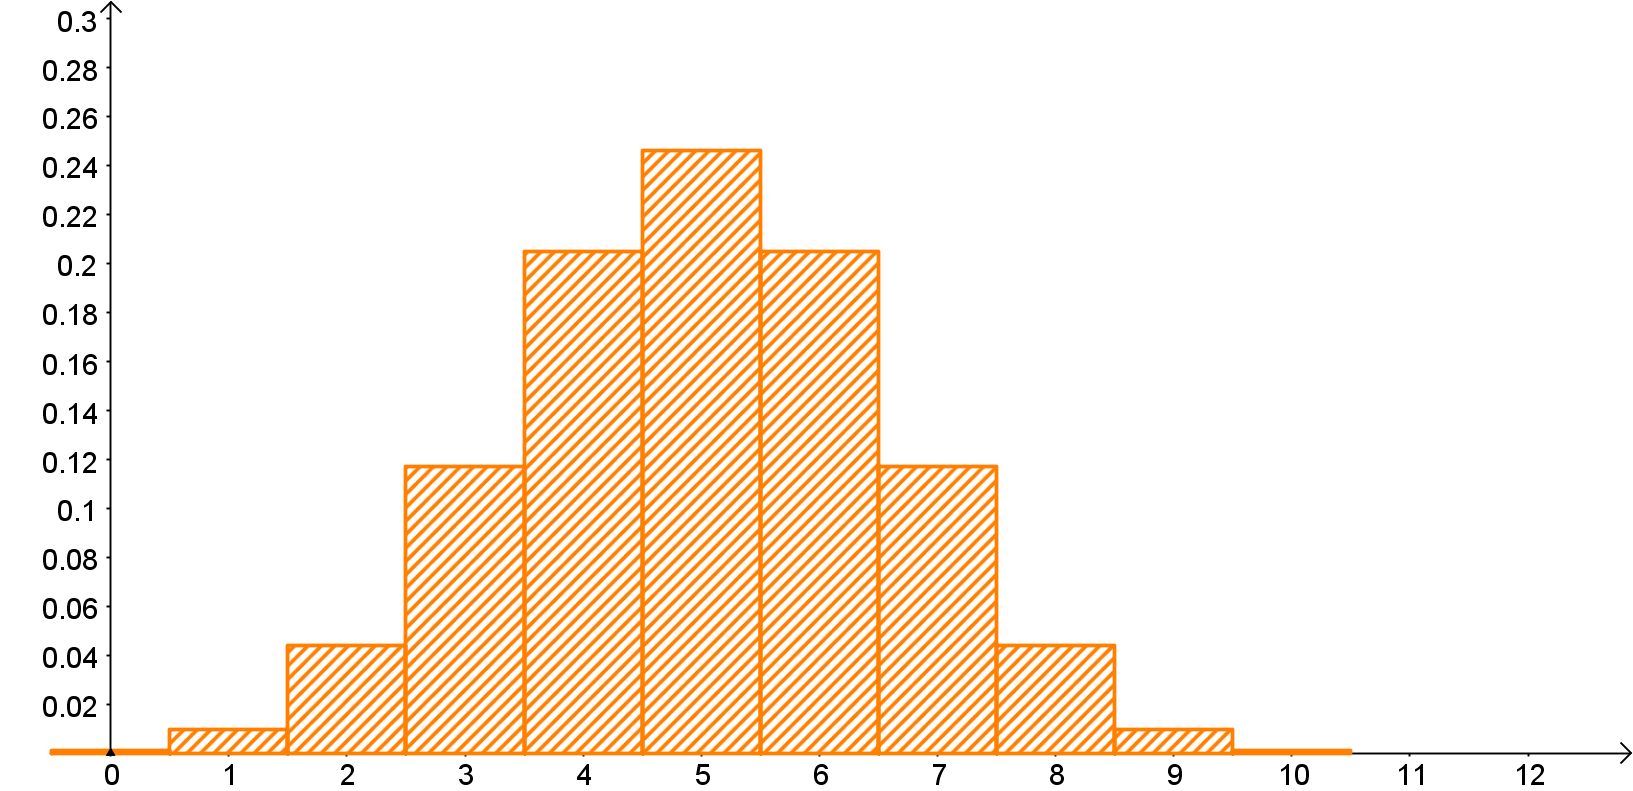
\includegraphics[width=11.5cm]{../fig/Cap05-ZooBinomial01.png}\\[3mm]
    (b)\\
    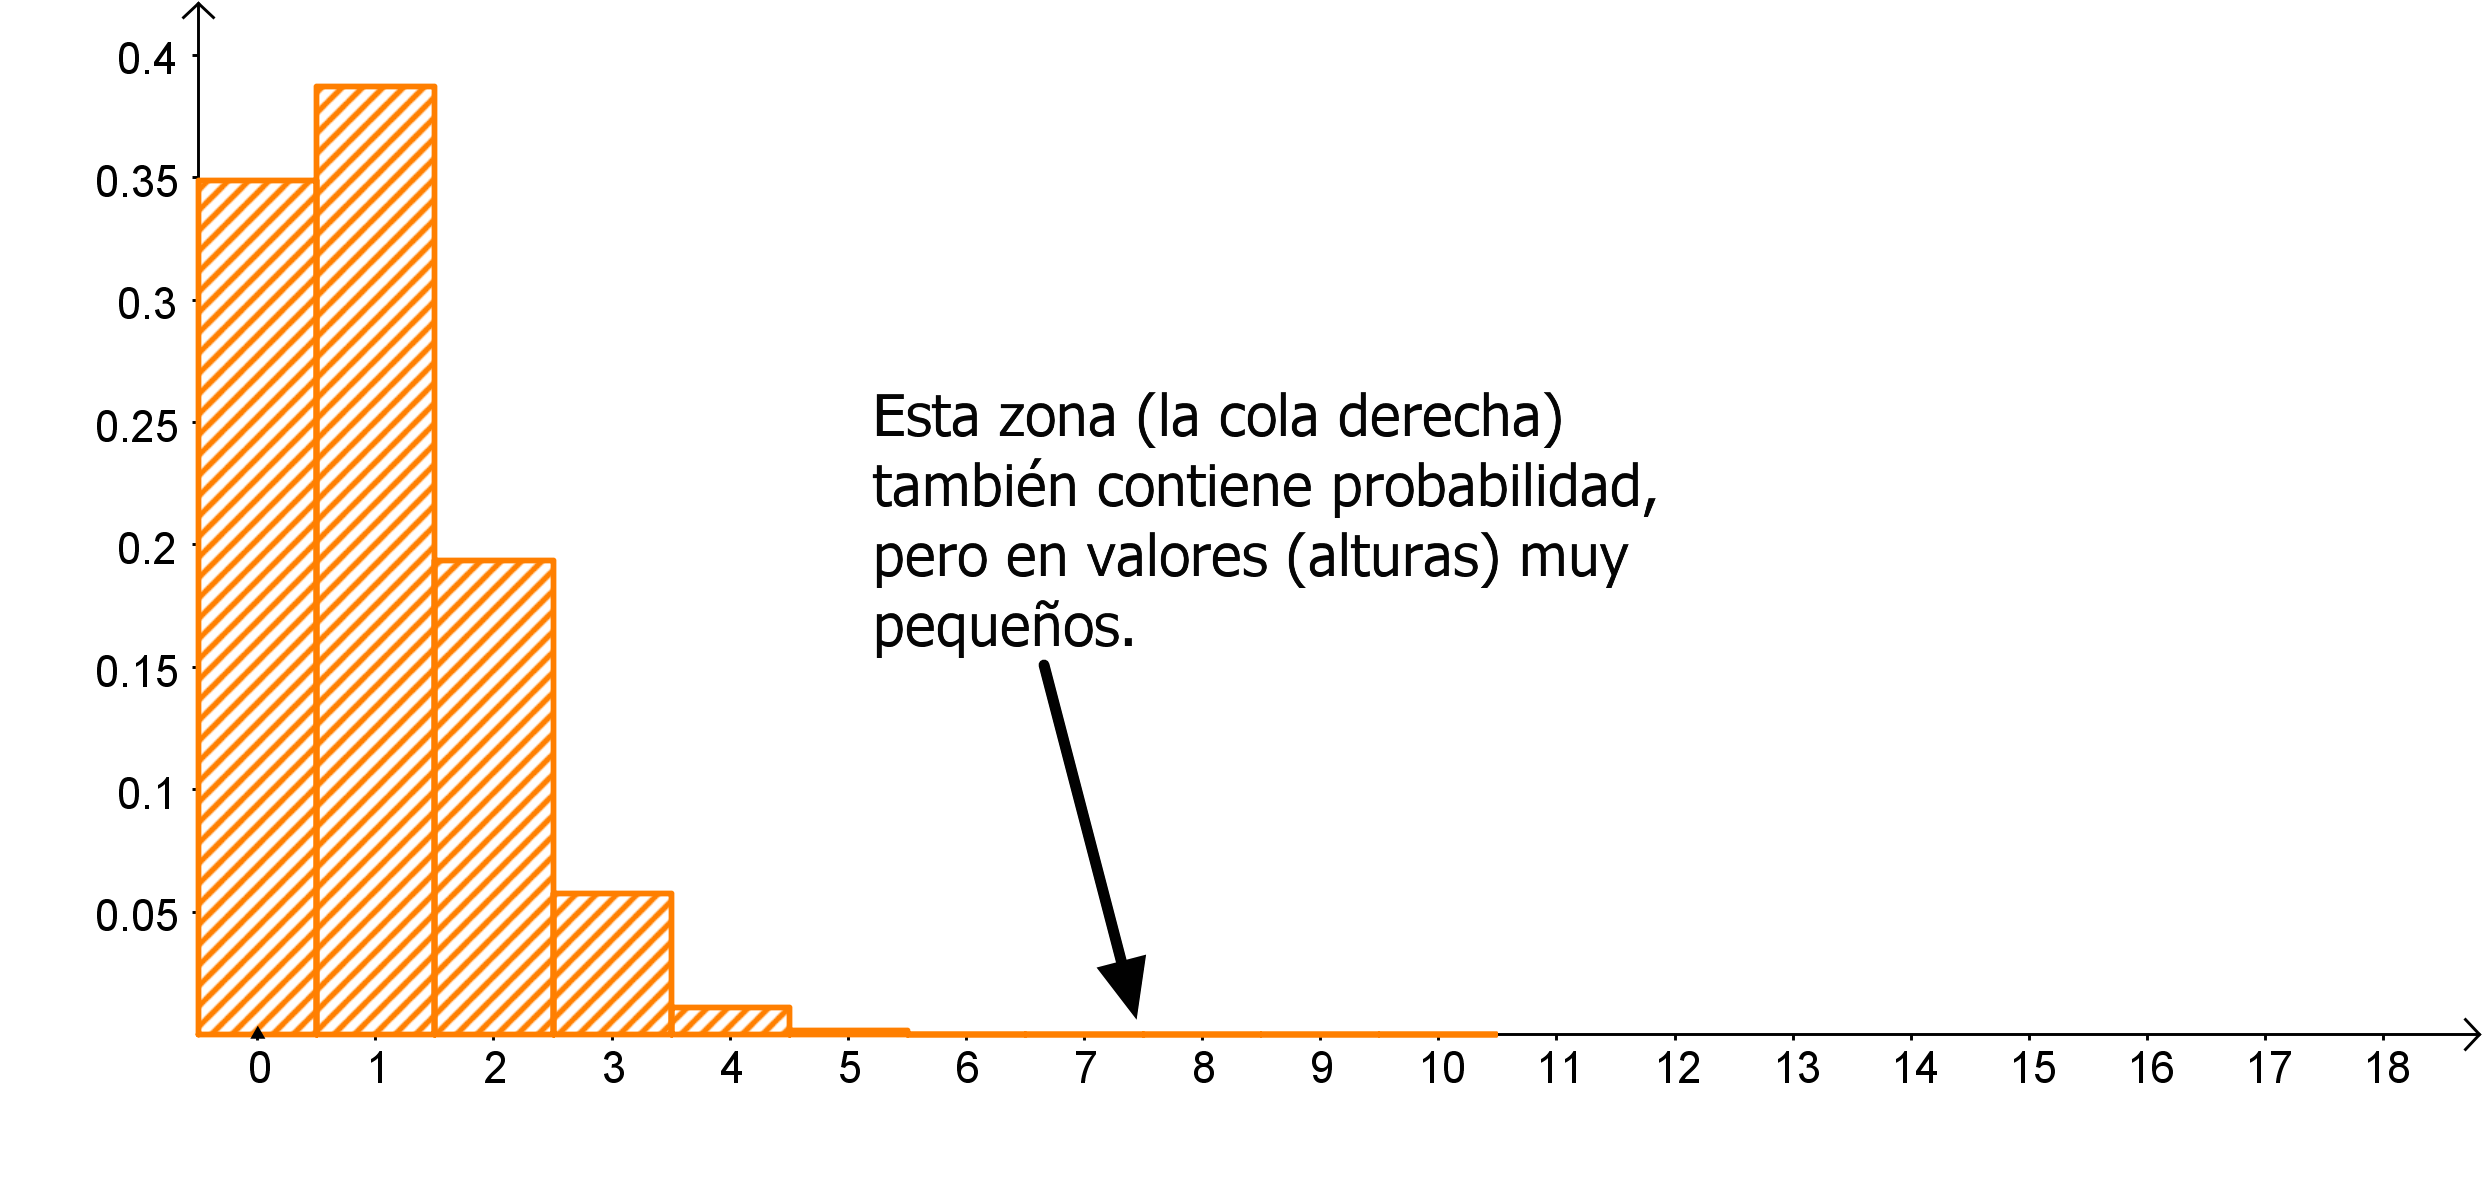
\includegraphics[width=11.5cm]{../fig/Cap05-ZooBinomial02.png}\\[3mm]
    (c)\\
    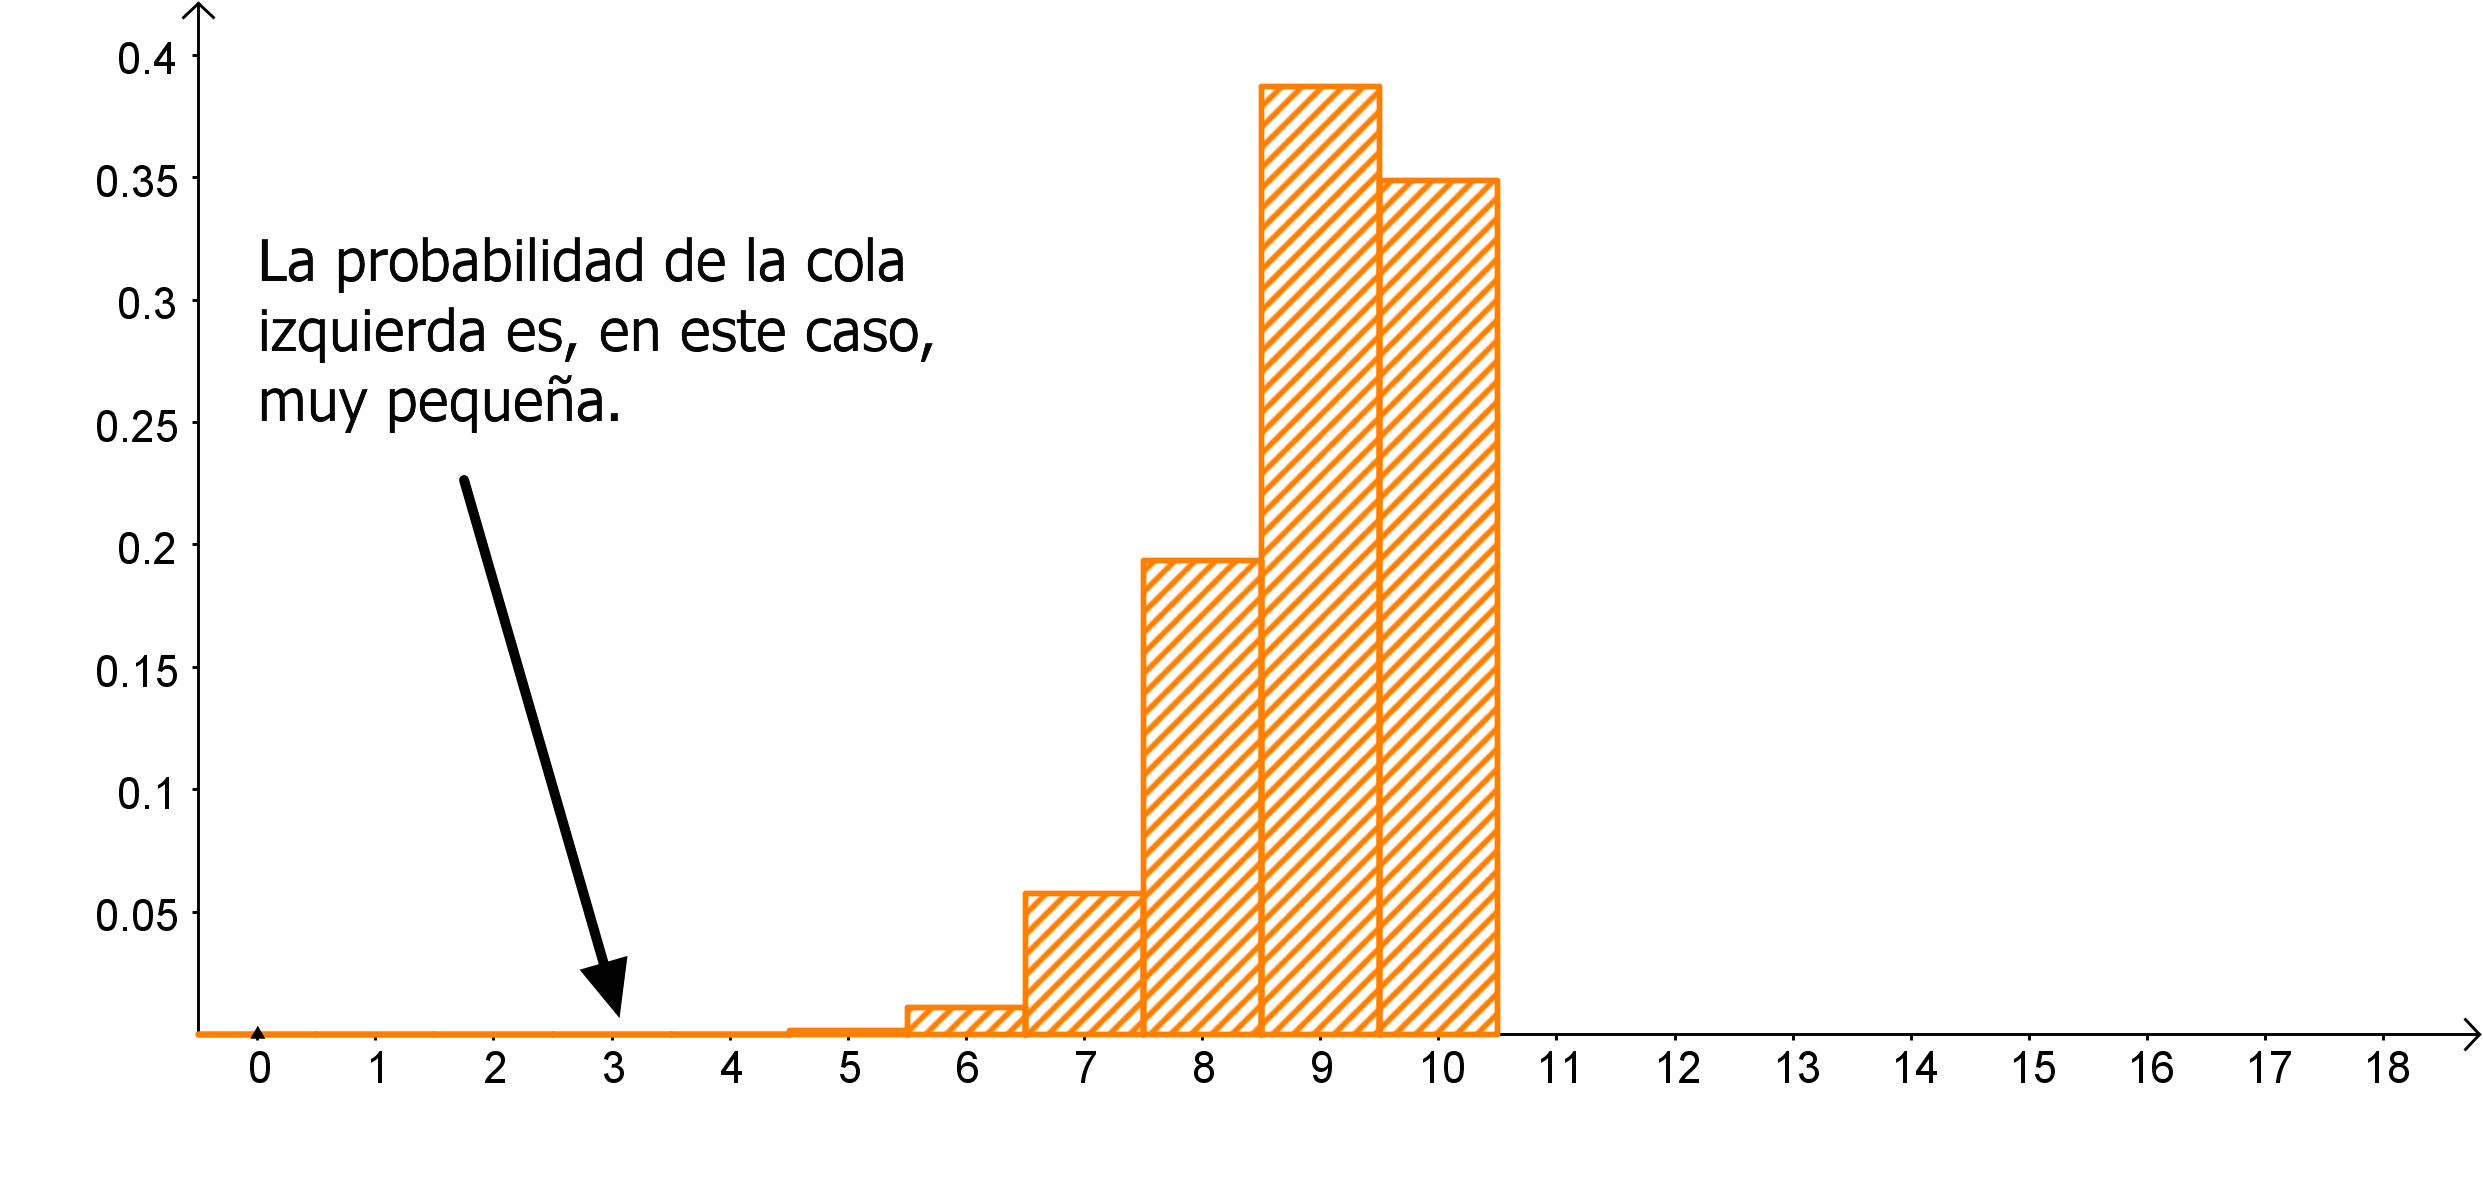
\includegraphics[width=11.5cm]{../fig/Cap05-ZooBinomial03.png}\\
	\end{enColor}
	\begin{bn}
    (a)\\
	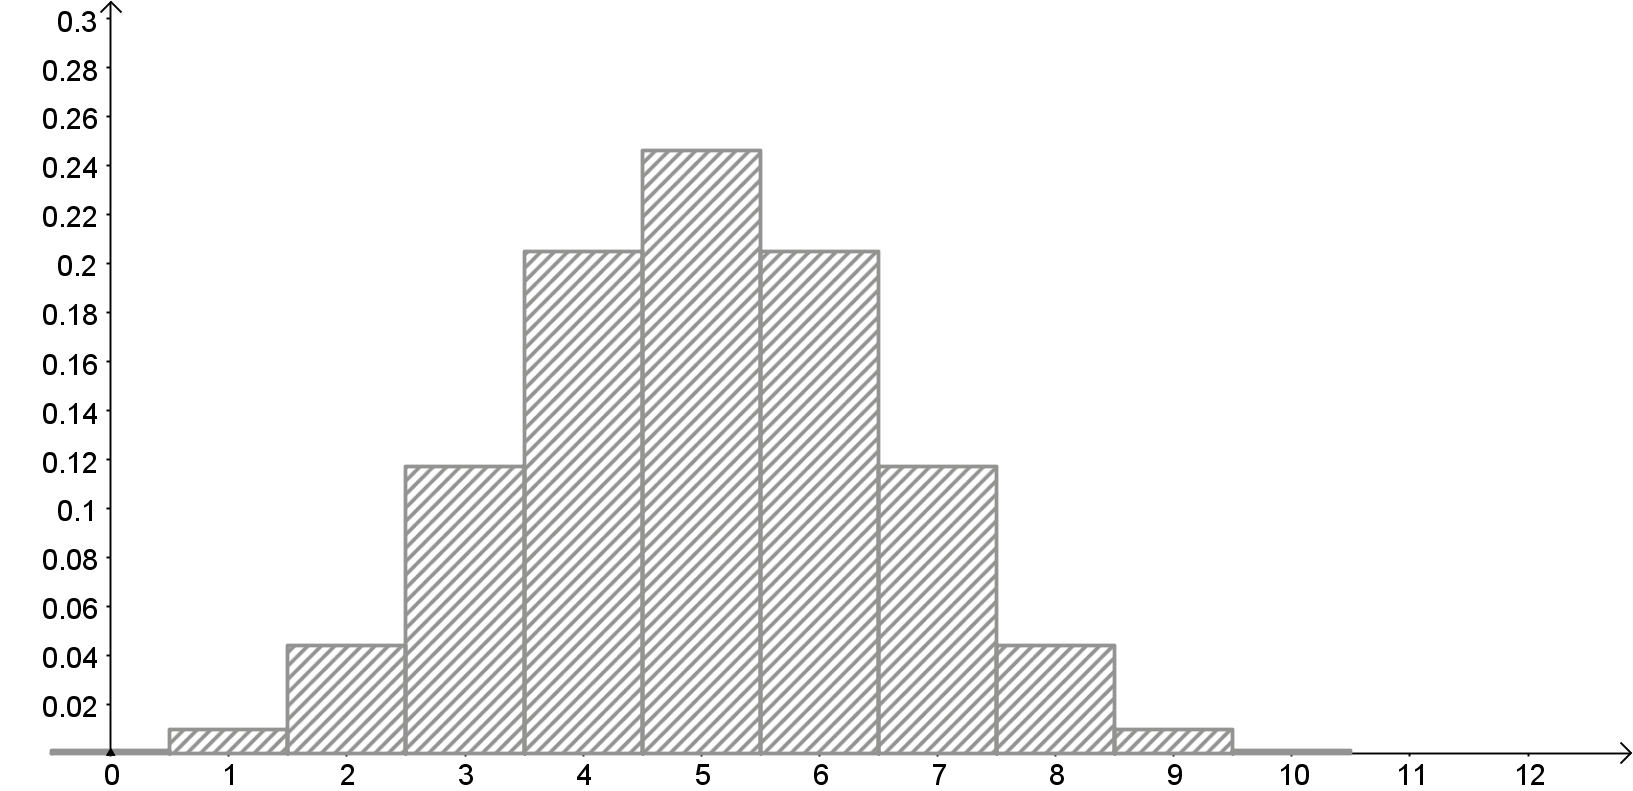
\includegraphics[width=11.5cm]{../fig/Cap05-ZooBinomial01-bn.png}\\[3mm]
    (b)\\
    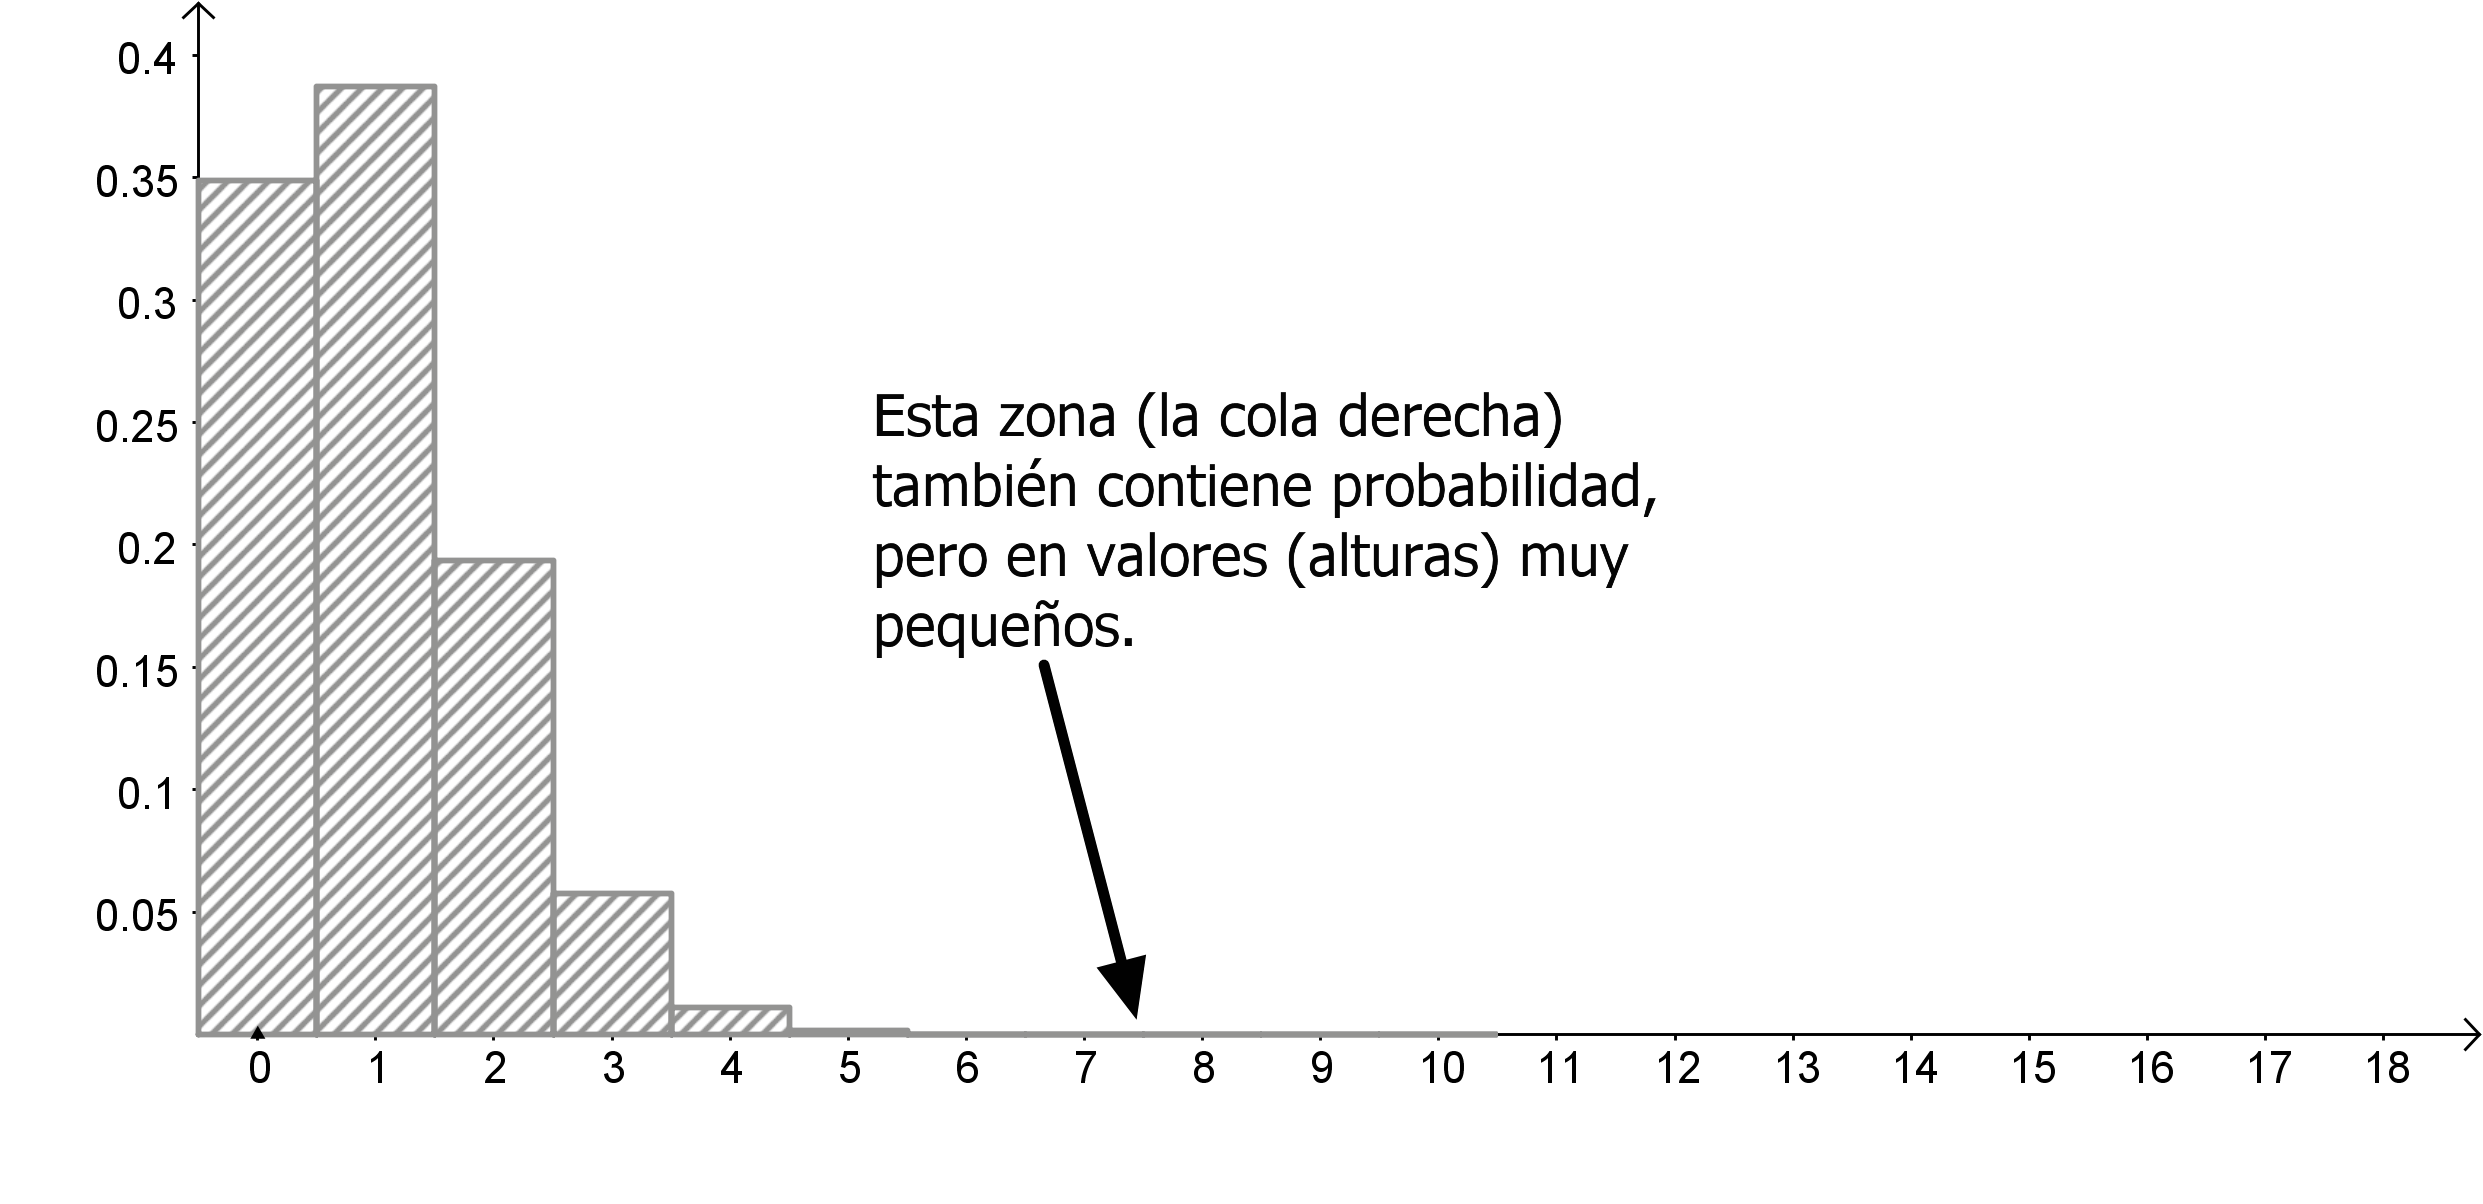
\includegraphics[width=11.5cm]{../fig/Cap05-ZooBinomial02-bn.png}\\[3mm]
    (c)\\
    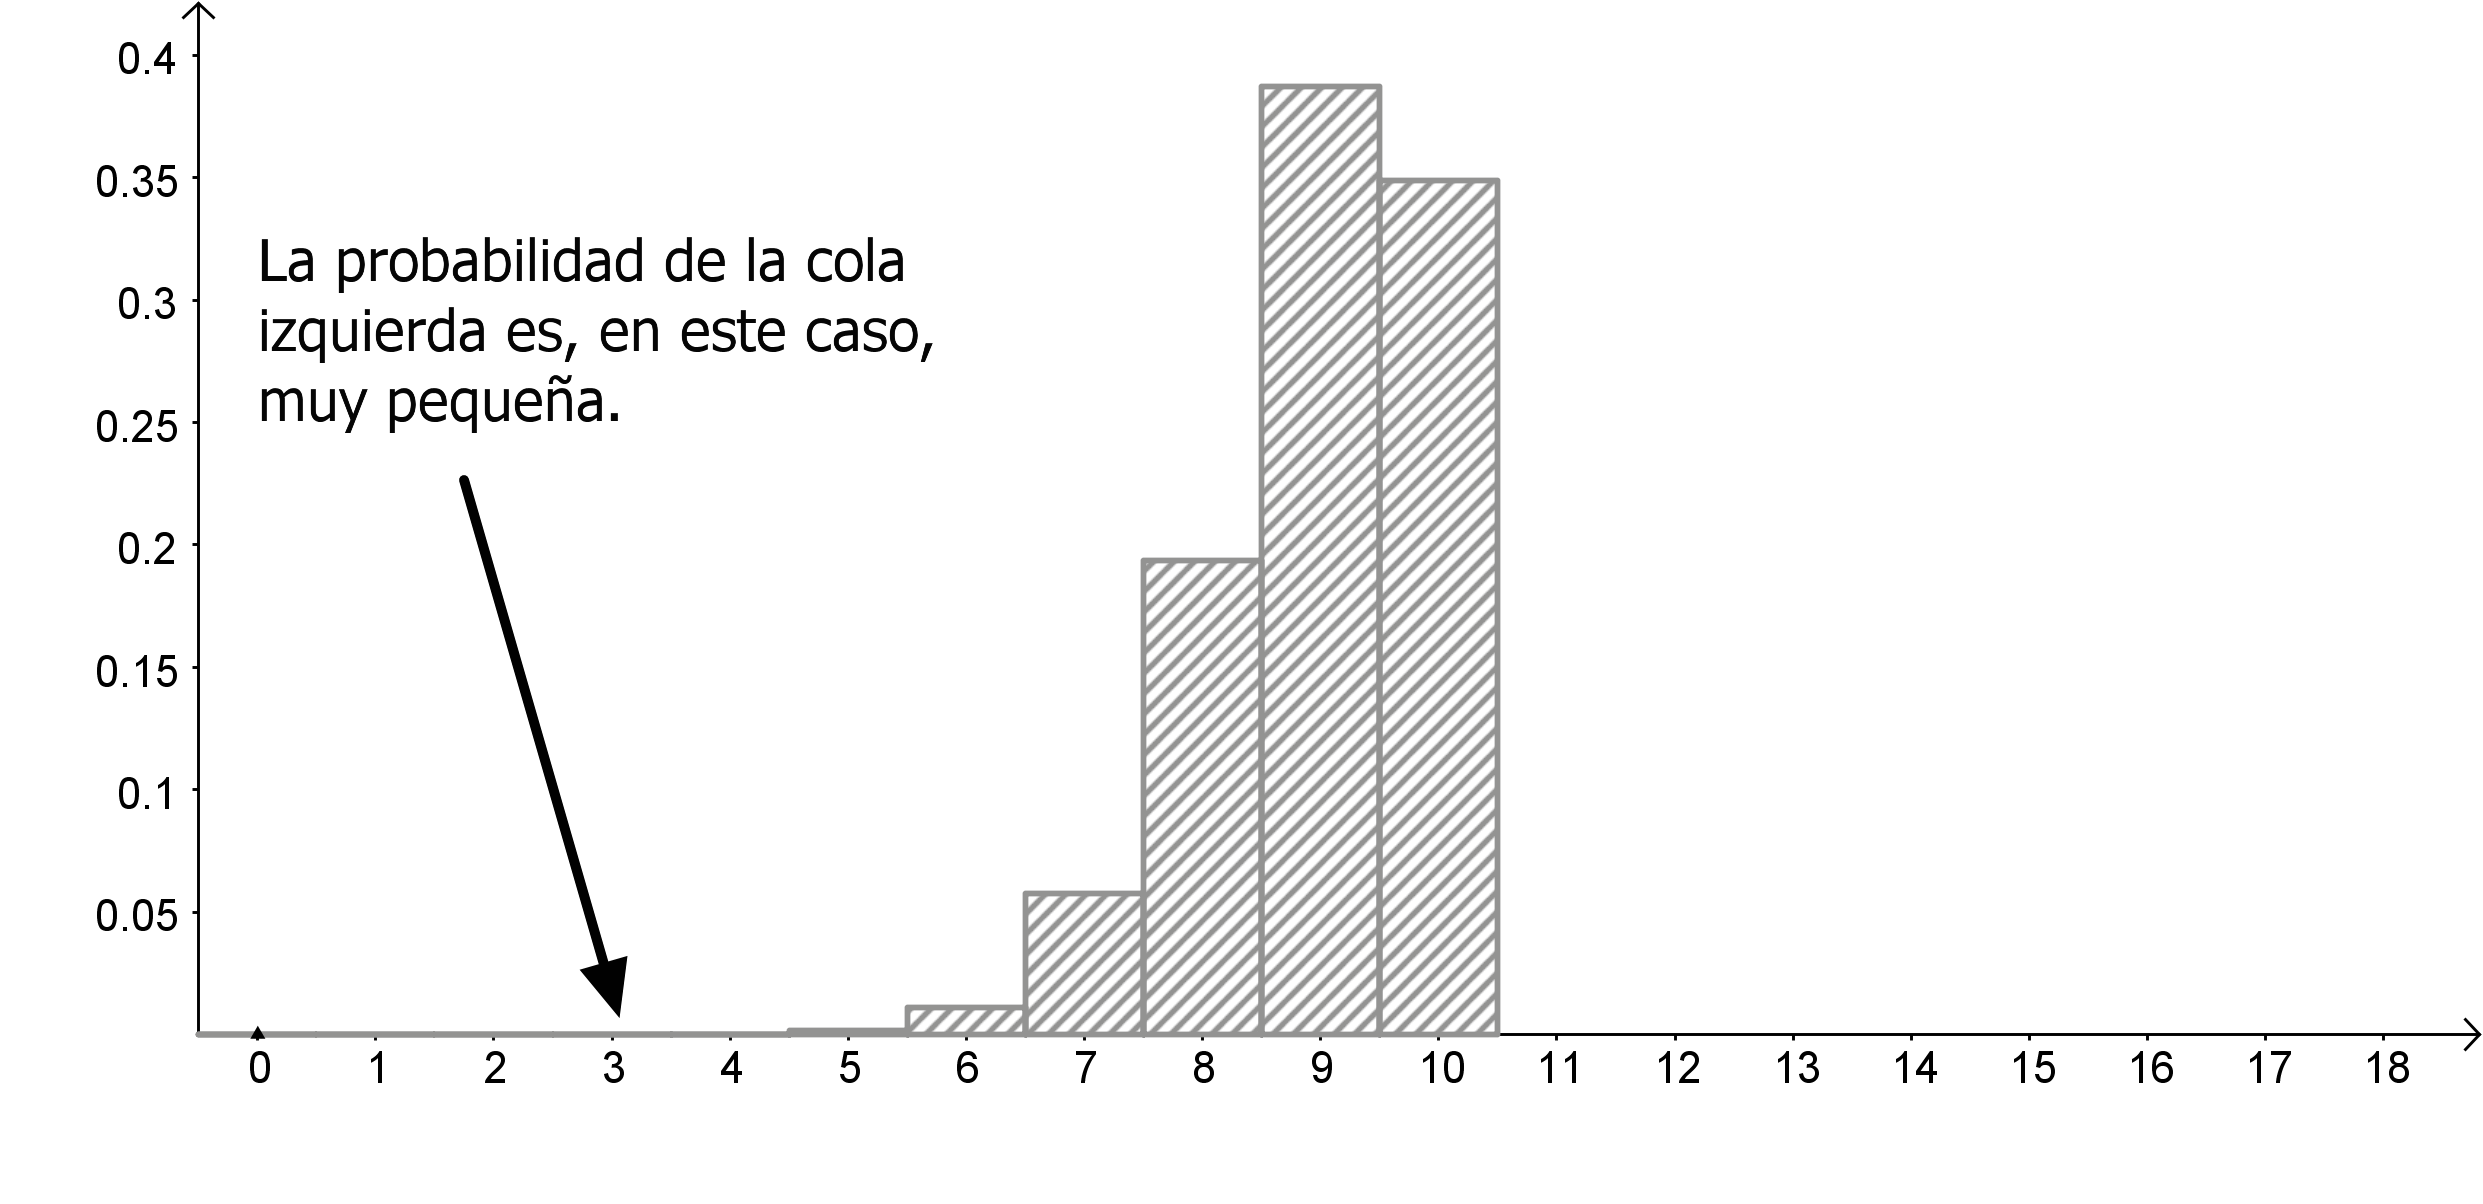
\includegraphics[width=11.5cm]{../fig/Cap05-ZooBinomial03-bn.png}\\
	\end{bn}
	\caption{Distribución Binomiales: (a)  $B(10,\frac{1}{2})$.  (b) $B(10,\frac{1}{10})$.
    (c) $B(10,\frac{9}{10})$.}
	\label{cap01:fig:ZooBinomial01}
    \end{center}
  \end{figure}

En las tres binomiales de la Figura \ref{cap01:fig:ZooBinomial01} hemos mantenido un valor bastante
bajo ($n=10$) del número de ensayos. Para valores de $n$ de este tamaño, los cálculos directos con
la binomial, usando su función de densidad (Ecuación
\ref{cap05:ecu:FuncionDensidadVariableBinomial}, pág.
\pageref{cap05:ecu:FuncionDensidadVariableBinomial}), aunque resultan tediosos en extremo, se
pueden todavía hacer a mano. Pero a partir de, por decir algo, $n=50$, casi cualquier cálculo
resulta insufriblemente complicado. Y sin embargo, $n=50$ no es un número muy grande, en términos
de las posibles aplicaciones de la binomial a los problemas del mundo real. Por eso, en la próxima
sección vamos a ocuparnos de lo que sucede cuando se consideran valores de $n$ cada vez más
grandes. Como aperitivo, y siguiendo con el énfasis en la {\em forma} de la distribución podemos
invitar al lector a que eche un vistazo por adelantado a la parte (b) de la Figura
\ref{cap05:fig:HistogramaBinomial02} (pág. \pageref{cap05:fig:HistogramaBinomial02}), en la que
aparece la distribución Binomial $B(100,\frac{1}{3})$. Como decíamos, en la próxima sección vamos a
dedicarnos al estudio de las distribuciones binomiales con valores de $n$ grandes. Esencialmente,
las distribuciones binomiales se pueden agrupar, para su estudio, en estas tres posibles
situaciones:

\begin{enumerate}
  \item Binomiales con $n$ pequeño, sea cual sea el valor de $p$. En estos casos, la receta suele
      pasar por emplear directamente la función de densidad de la Ecuación Ecuación
      \ref{cap05:ecu:FuncionDensidadVariableBinomial} (pág.
      \pageref{cap05:ecu:FuncionDensidadVariableBinomial}).
  \item Binomiales con $n$ grande (ya precisaremos qué significa eso), y con valor moderado de
      $p$; ni demasiado pequeño (cercano a $0$), ni demasiado grande (cercano a $1$). Estos son
      los casos de los que nos ocuparemos en las próximas secciones.
  \item El caso restante, es aquel en el que $n$ es grande, pero los valores de $p$ son muy
      pequeños, o muy cercanos a $1$ (estos dos casos son similares, basta intercambiar los
      papeles de $p$ y $q$). Para darle al lector una idea del aspecto de las distribuciones en
      este caso, hemos representado la binomial $B(1000,\dfrac{1}{10000})$ en la Figura
      \ref{cap01:fig:ZooBinomial04}.

  \begin{figure}[hbt]
	\begin{center}
	\begin{enColor}
	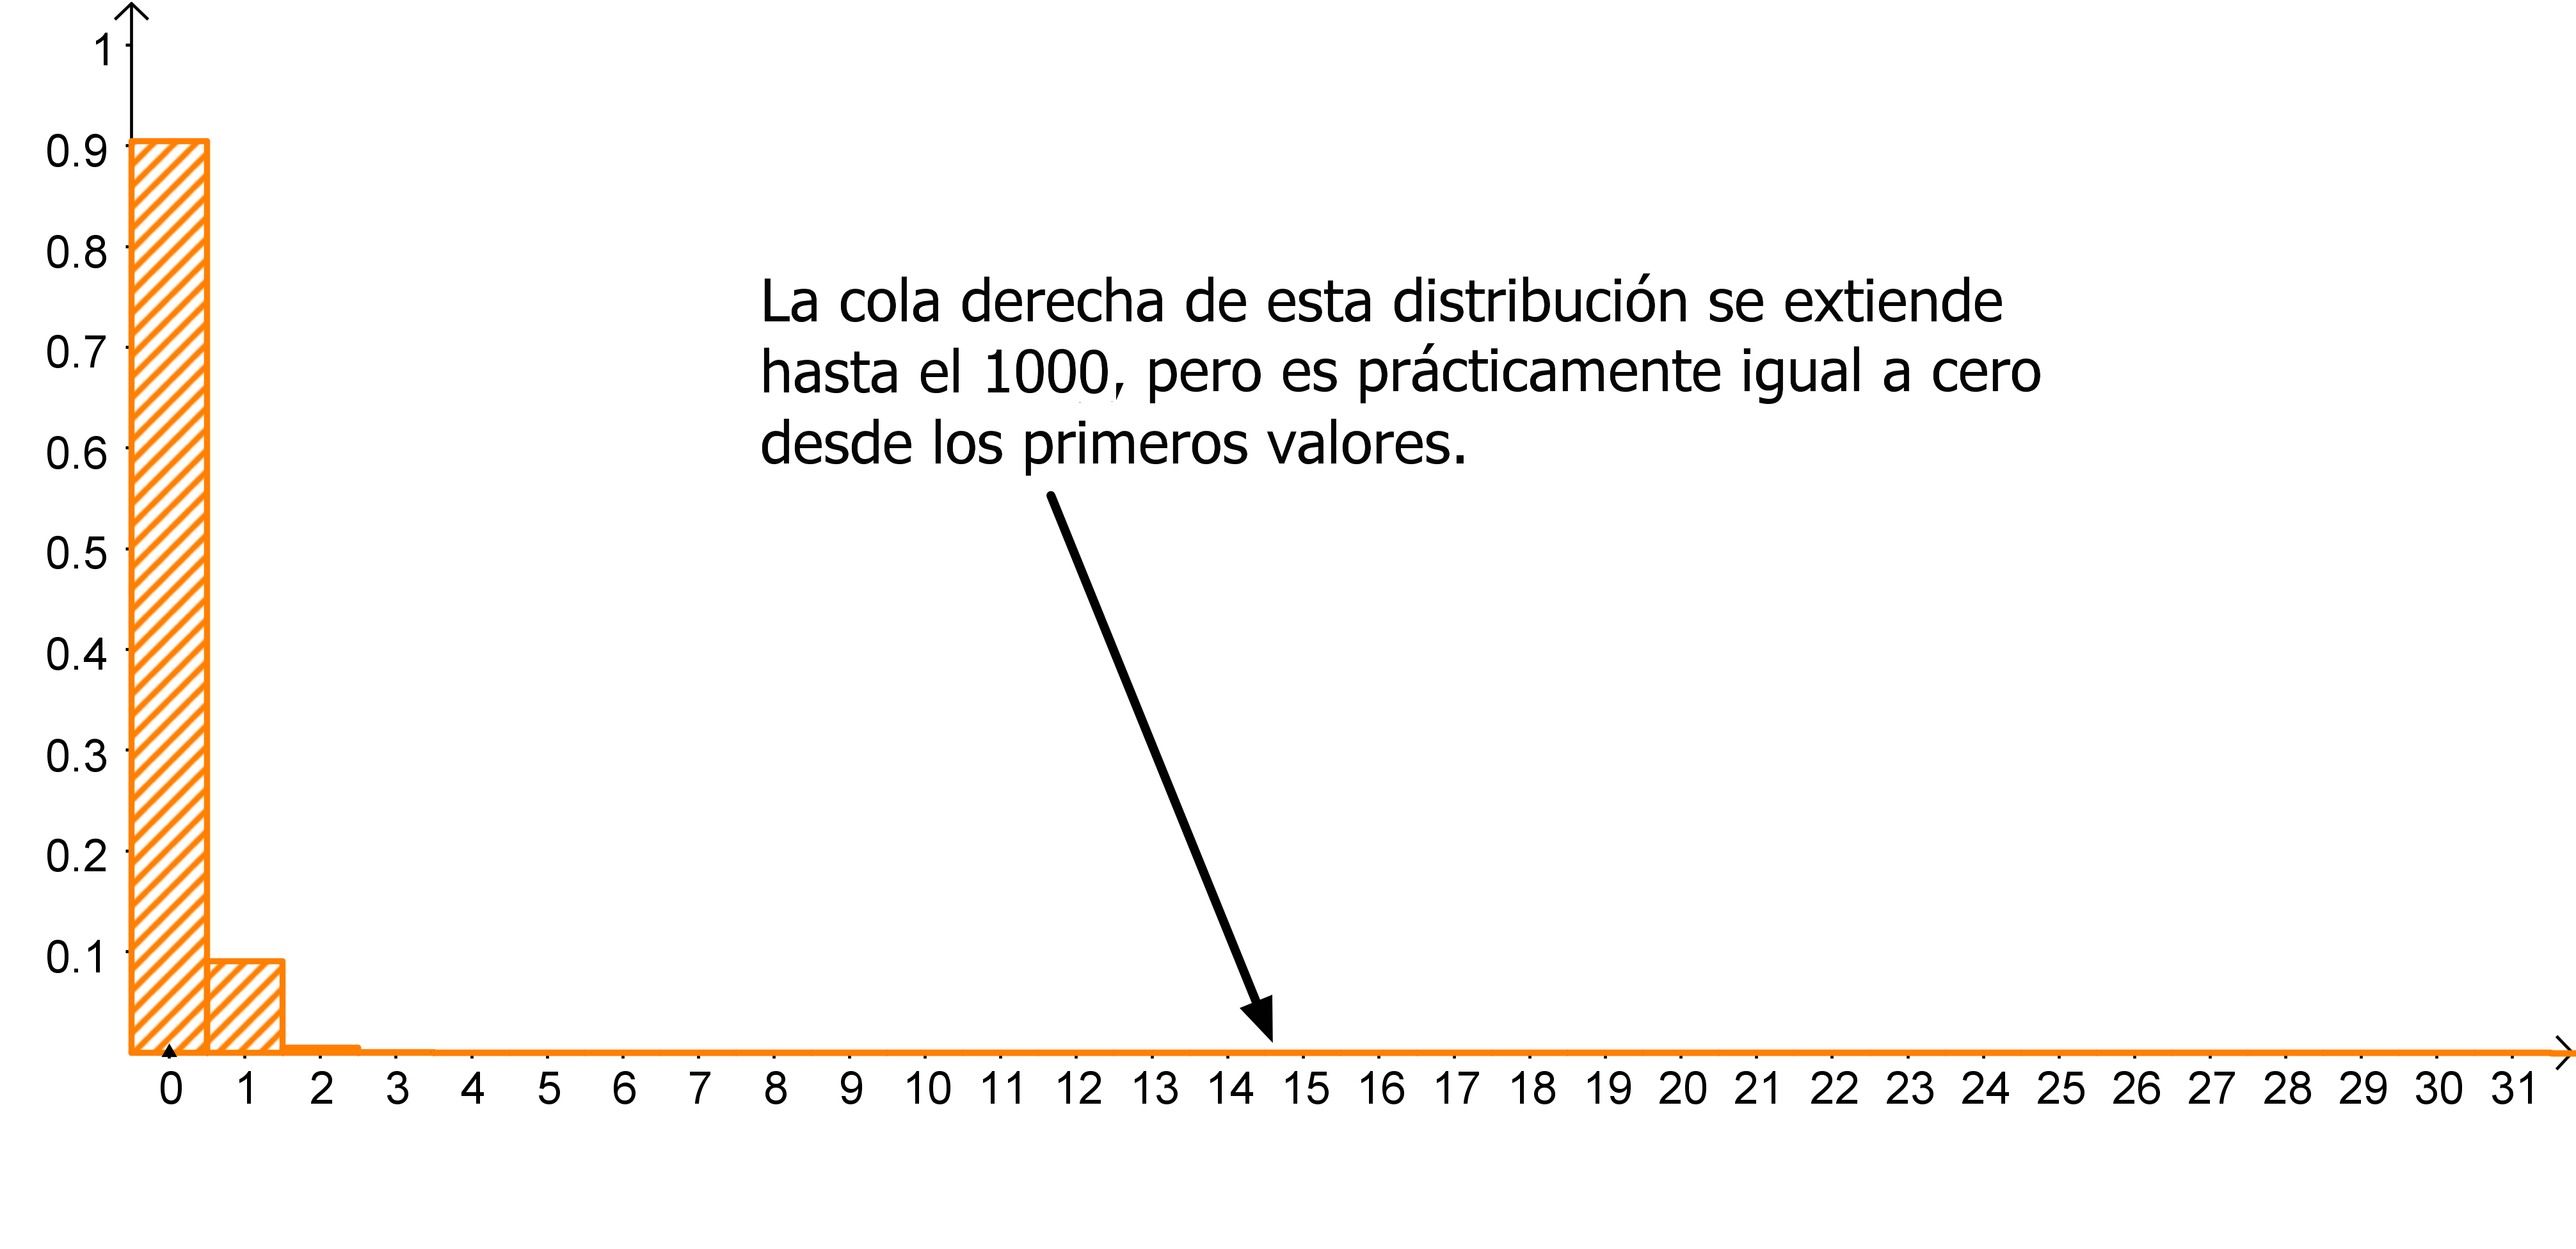
\includegraphics[width=11.5cm]{../fig/Cap05-ZooBinomial04.png}
	\end{enColor}
	\begin{bn}
	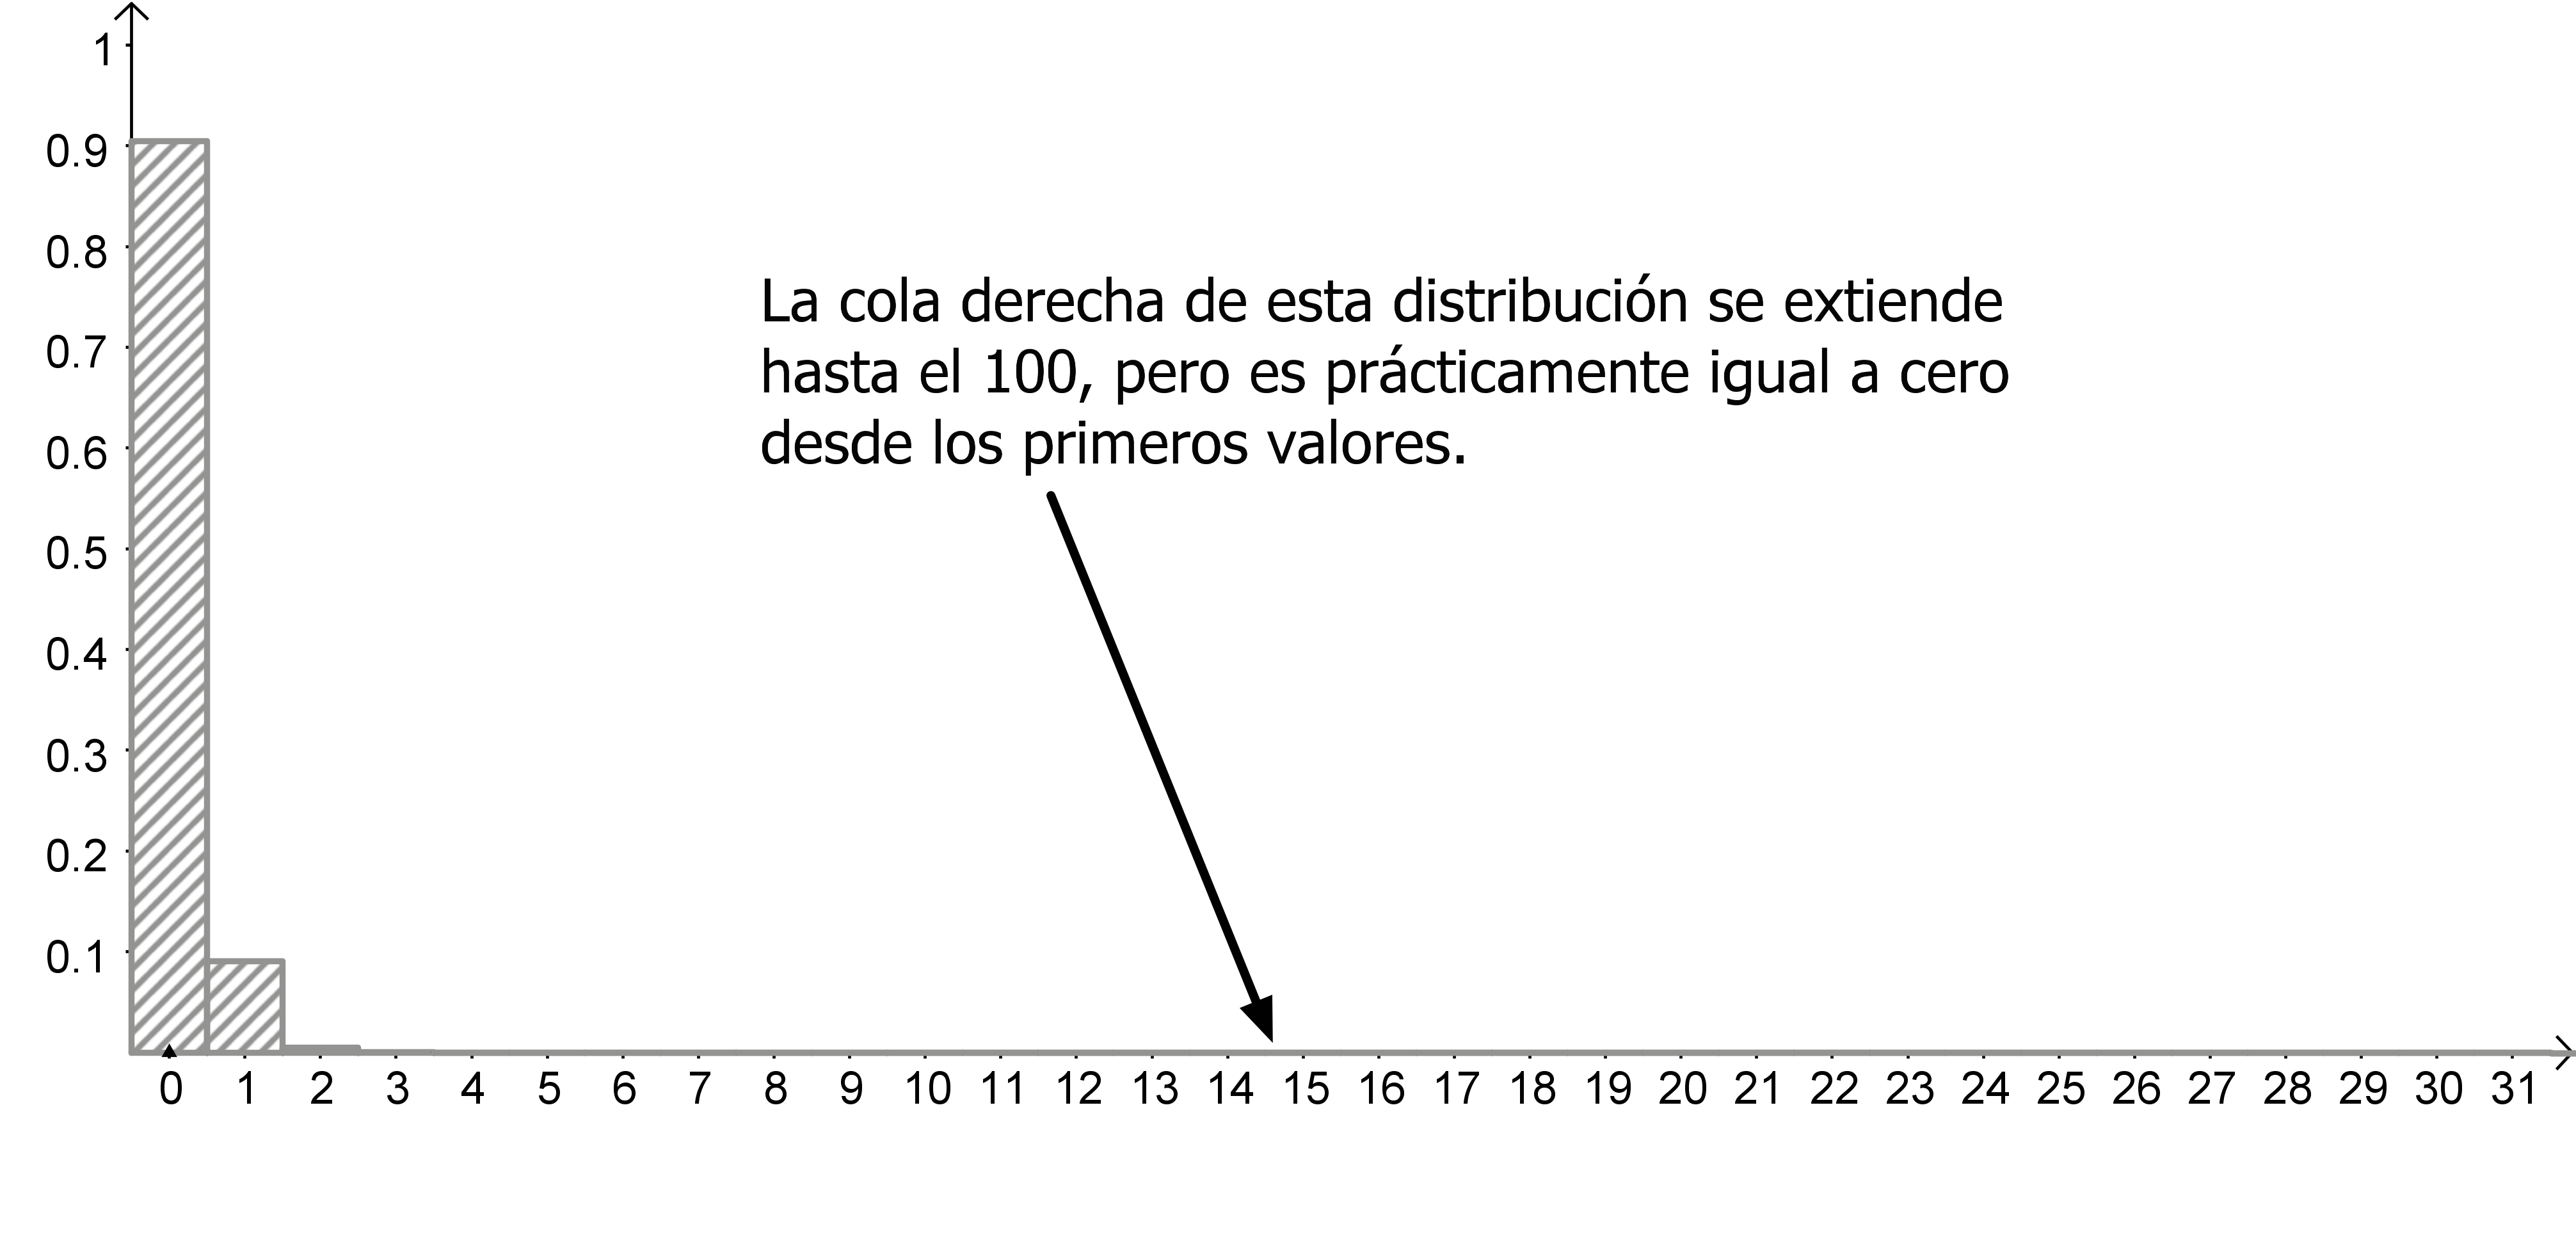
\includegraphics[width=11.5cm]{../fig/Cap05-ZooBinomial04-bn.png}
	\end{bn}
	\caption{Distribución Binomial: $B\left(1000,\dfrac{1}{10000}\right)$.}
	\label{cap01:fig:ZooBinomial04}
    \end{center}
  \end{figure}


      Como puede verse, estas distribuciones son un caso extremo, que concentra casi toda la probabilidad en los valores iniciales (o finales, si $p\approx 1$), en muy pocos valores, si se comparan con $n$ (que, en este ejemplo, es $100$). Este es el caso más difícil de tratar, y de hecho lo vamos a apartar de nuestra discusión hasta la Sección \ref{cap08:sec:DistribucionPoisson} del Capítulo \ref{cap:DistribucionesRelacionadasBinomial} (pág. \pageref{cap08:sec:DistribucionPoisson}), cuando estudiaremos la distribución de Poisson, que está hecha a la medida de esta situación.
\end{enumerate}

Naturalmente, hay distribuciones que no son binomiales, y a veces basta con echar un vistazo a una gráfica de frecuencias observadas, y compararla con la gráfica teórica de probabilidades, para comprender que estamos ante una distribución que no es binomial. La Figura \ref{cap02:fig:DatosBimodales} (pág. \pageref{cap02:fig:DatosBimodales}), por ejemplo, muestra las frecuencias observadas de un conjunto de datos {\em bimodal}\index{bimodal}, con dos máximos bien diferenciados de la frecuencia. Y las distribuciones binomiales nunca son bimodales, así que la distribución de la variable, en la población de la que se ha tomado esa muestra, no parece una binomial. Una gráfica bimodal nos puede hacer sospechar que los datos que estamos observando provienen, en realidad, de la mezcla de dos poblaciones distintas, correspondientes a los dos máximos de la frecuencia.

\section{Distribuciones Binomiales con n muy grande.}\label{sec:DistribucionesBinomialesnGrande}


\noindent{\em ``If I have seen further, it is by standing upon the shoulders of giants''.\\ Isaac
Newton, 1676}.\\

Cuando los matemáticos empezaron a trabajar con la distribución binomial, no había ordenadores (ni calculadoras) disponibles. En esas condiciones, incluso el cálculo de un valor relativamente sencillo $P(X=30)$ para la distribución binomial $B(100,1/3)$, implicaba calcular números como $\binom{100}{30}$ (que es del orden de $10^{25}$). Ese cálculo podía resultar un inconveniente casi insufrible. Por esa razón, aquellos matemáticos empezaron a pensar sobre el comportamiento de la distribución binomial para valores de $n$ cada vez más grandes. Entre esos matemáticos estaba Abraham De Moivre\index{De Moivre, Abraham}, un hugonote francés refugiado en Londres, que había pasado a formar parte del selecto grupo de personas cercanas a Isaac Newton\index{Newton, Isaac}. Esa cercanía a uno de los fundadores del Cálculo nos ayuda a imaginar (sin pretensión alguna de rigor histórico) cómo pudo llegar De Moivre a algunos de sus hallazgos.

Nos imaginamos que De Moivre empezó pensando en los valores de una distribución binomial $B(n,p)$ para $n$ pequeño, por ejemplo $n=10$, y un valor cualquiera de $p$, por ejemplo $p=1/3$.
Al representar los valores de probabilidad
\[P(X=0),\quad P(X=1),\quad P(X=2),\,\ldots\,,\quad P(X=10)\]
en un gráfico similar a un histograma se obtiene la parte (a) de la Figura \ref{cap05:fig:HistogramaBinomial02} (pág. \pageref{cap05:fig:HistogramaBinomial02}). En realidad es un gráfico de columnas, pero hemos eliminado el espacio entre las columnas, por razones que enseguida serán evidentes. Fíjate en que, además, a diferencia de los histogramas del Capítulo \ref{cap:IntroduccionEstadisticaDescriptiva}, en el eje vertical estamos representando probabilidades, en lugar de frecuencias. Y, en particular, eso hace que las escalas de los ejes sean muy distintas. De Moivre, probablemente, siguió pensando en este tipo de figuras para valores de $n$ cada vez más grandes. Por ejemplo, para $n=100$ se obtiene la parte (b) de la Figura \ref{cap05:fig:HistogramaBinomial02}.

%\newpage
%\begin{figure}[t]
%\begin{center}
%\begin{enColor}
%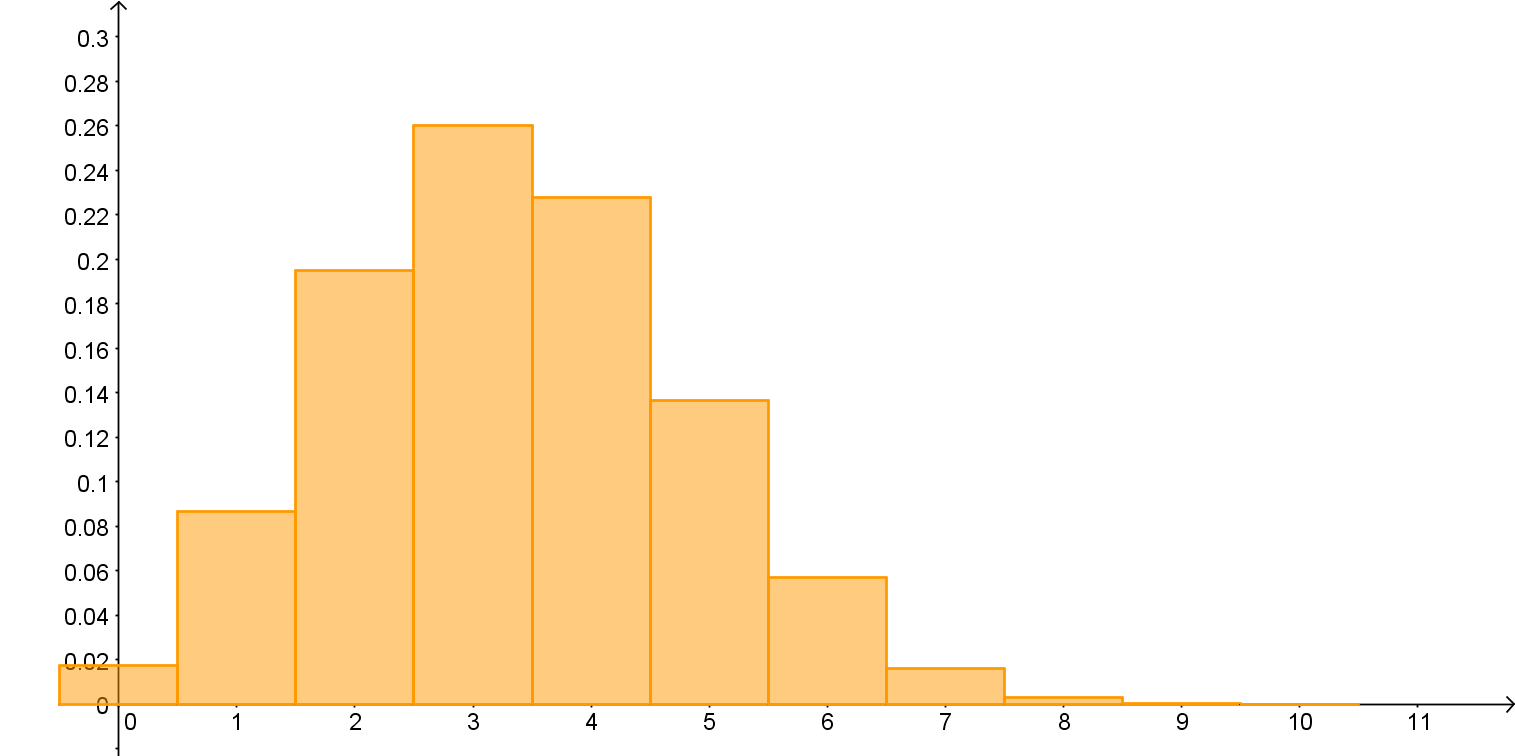
\includegraphics[width=9cm]{../fig/Cap05-HistogramaBinomial01.png}
%\end{enColor}
%\begin{bn}
%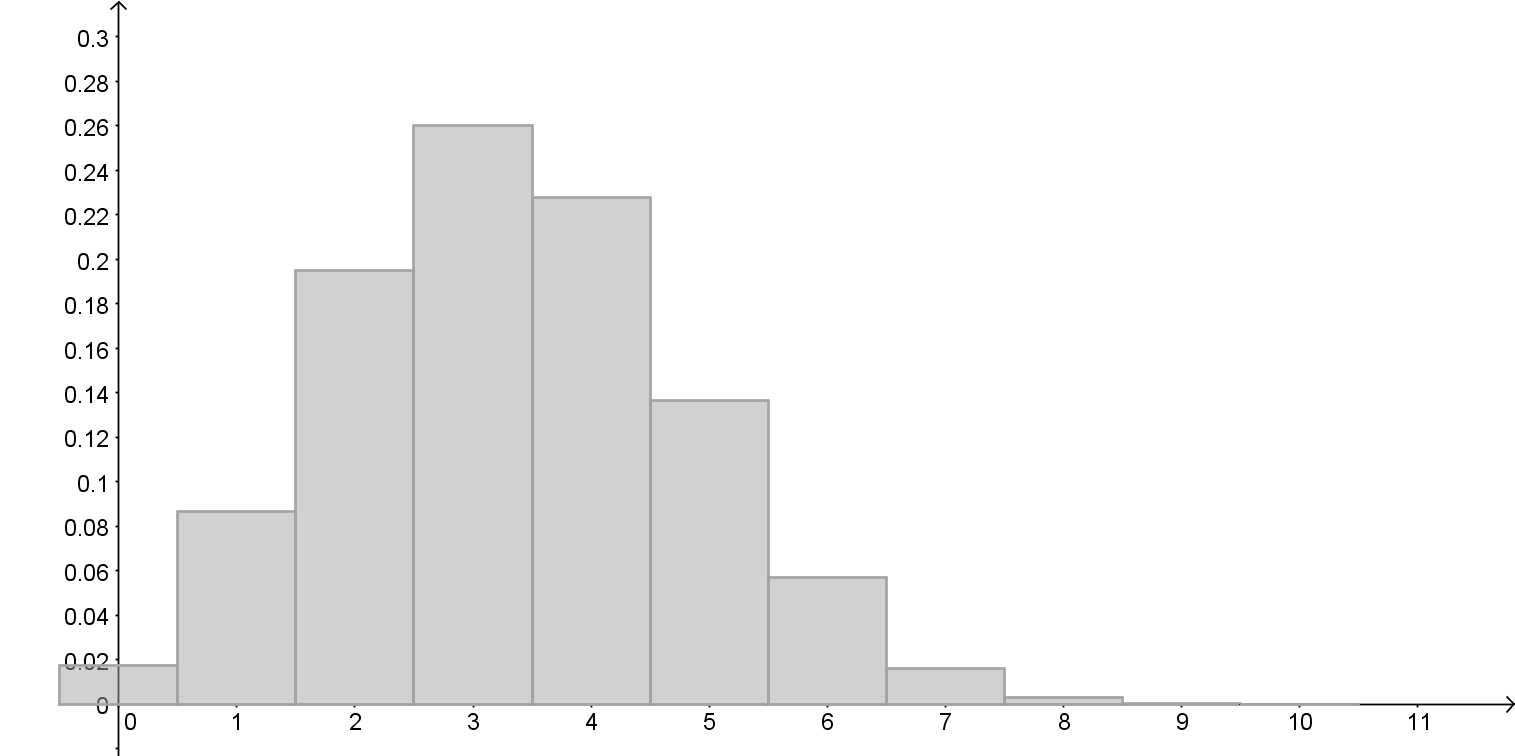
\includegraphics[width=9cm]{../fig/Cap05-HistogramaBinomial01-bn.png}
%\end{bn}
%\caption{La distribución de probabilidad binomial $B\left(10,\frac{1}{3}\right)$.}
%\label{cap05:fig:HistogramaBinomial01}
%\end{center}
%\end{figure}
\begin{figure}[p]
\begin{center}
\begin{enColor}
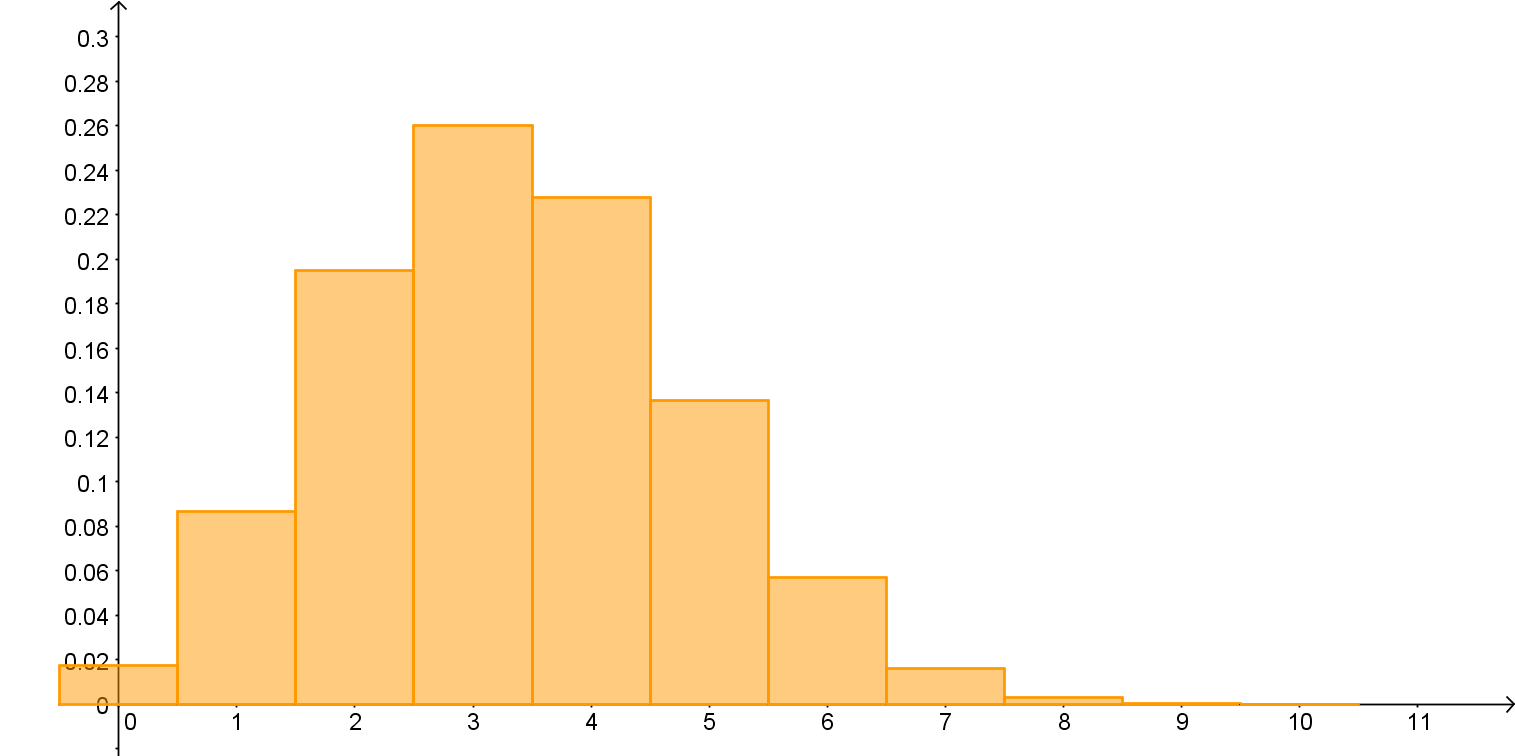
\includegraphics[width=9cm]{../fig/Cap05-HistogramaBinomial01.png}\\
(a)\\
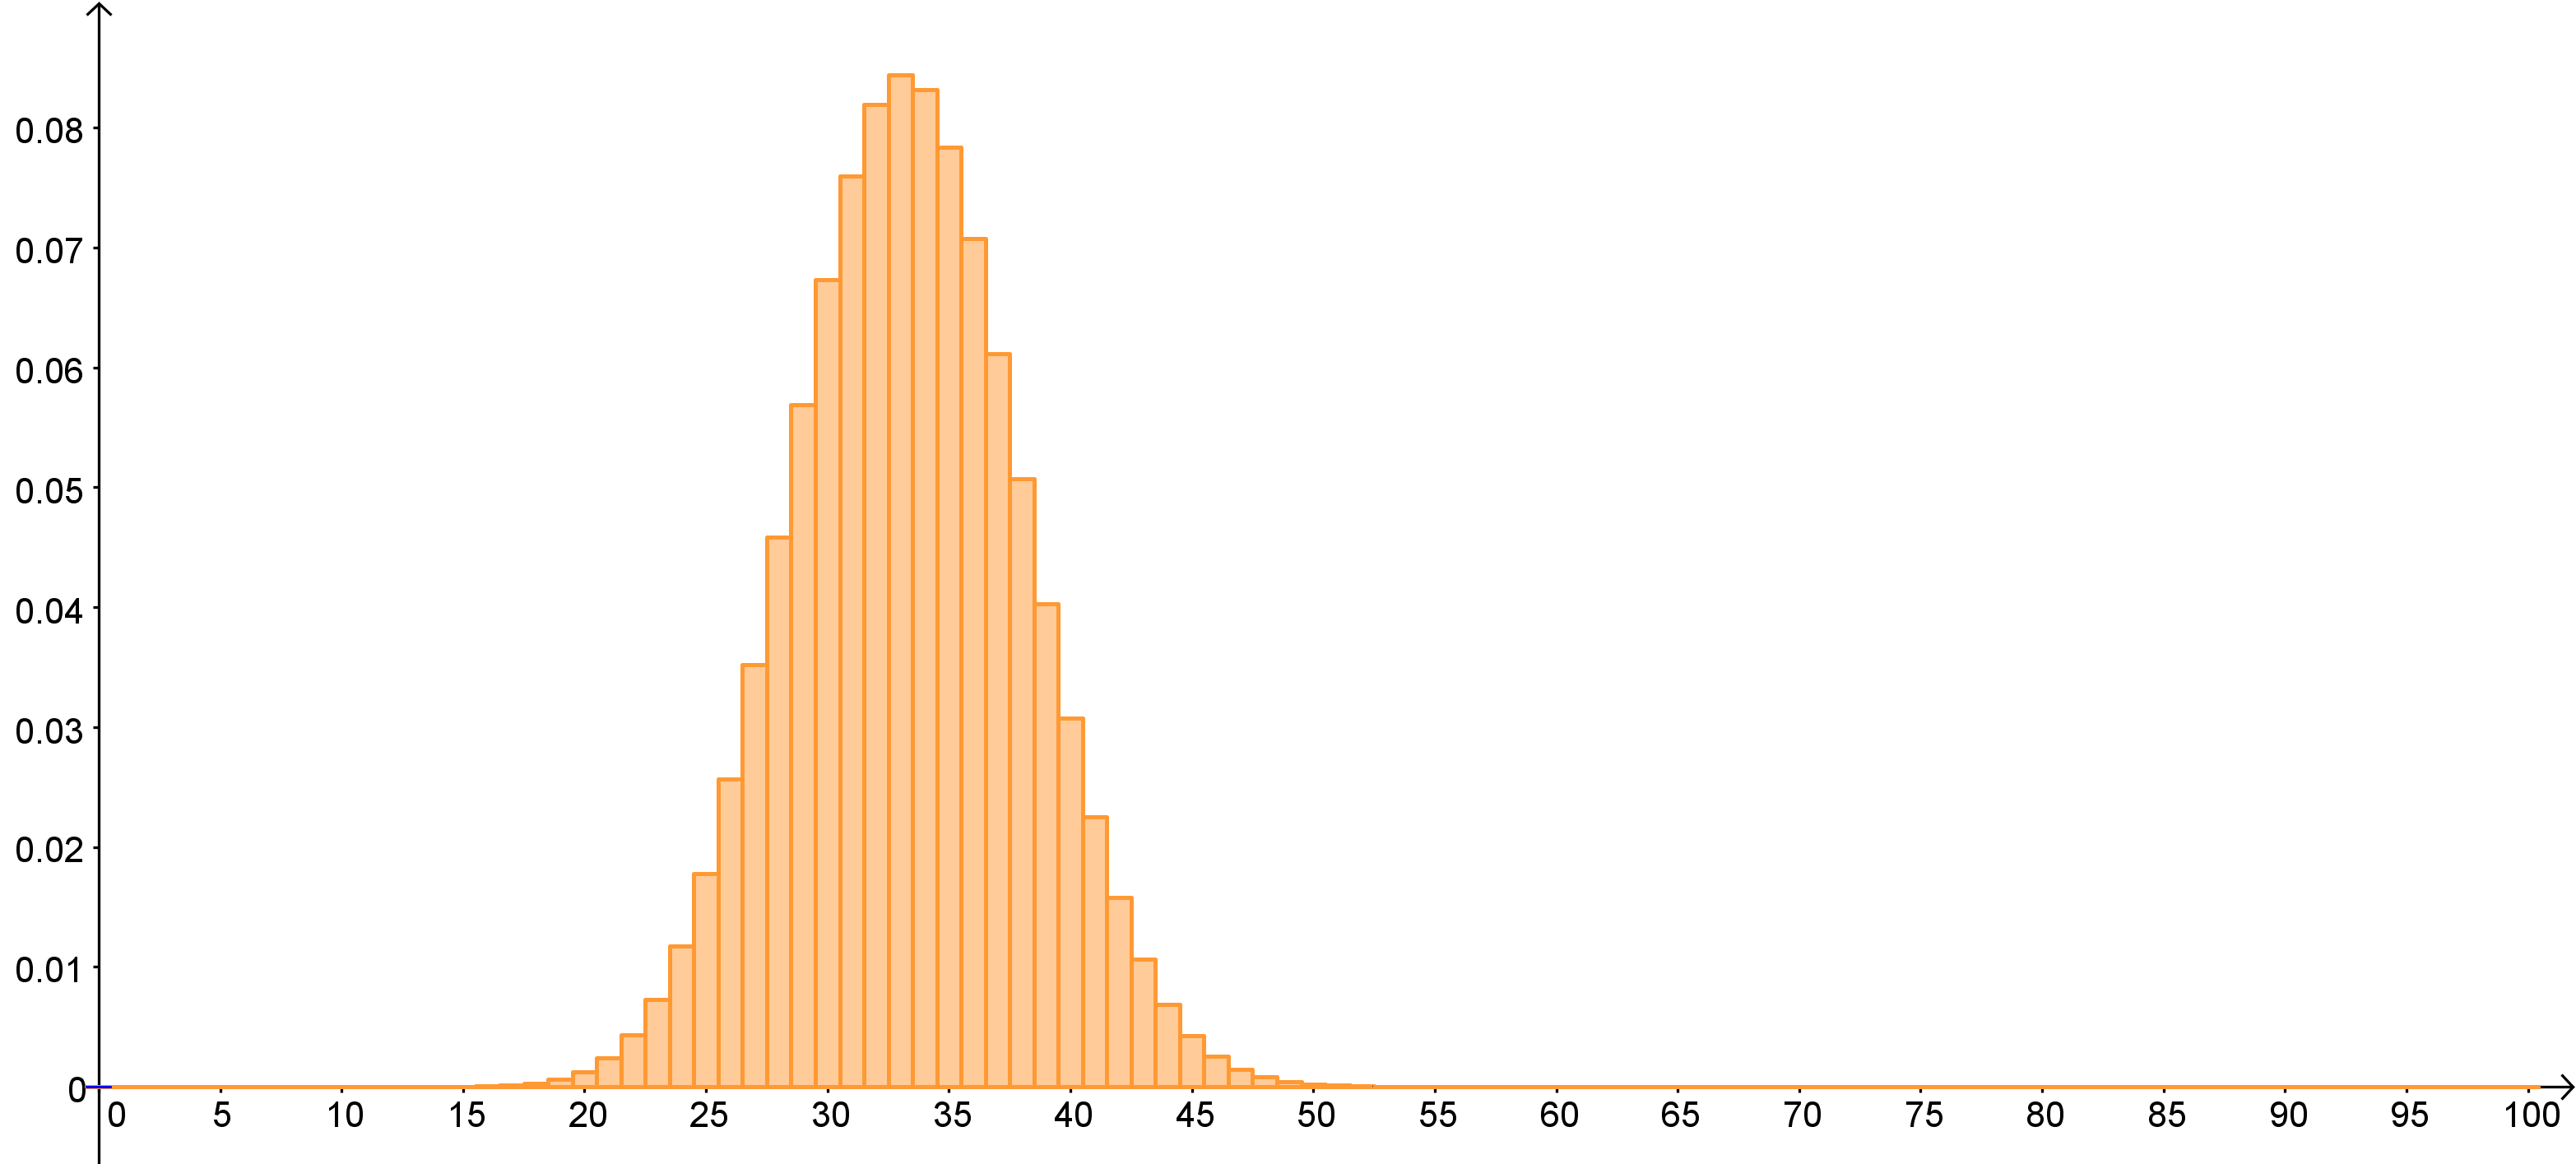
\includegraphics[width=9cm]{../fig/Cap05-HistogramaBinomial02.png}\\
(b)\\
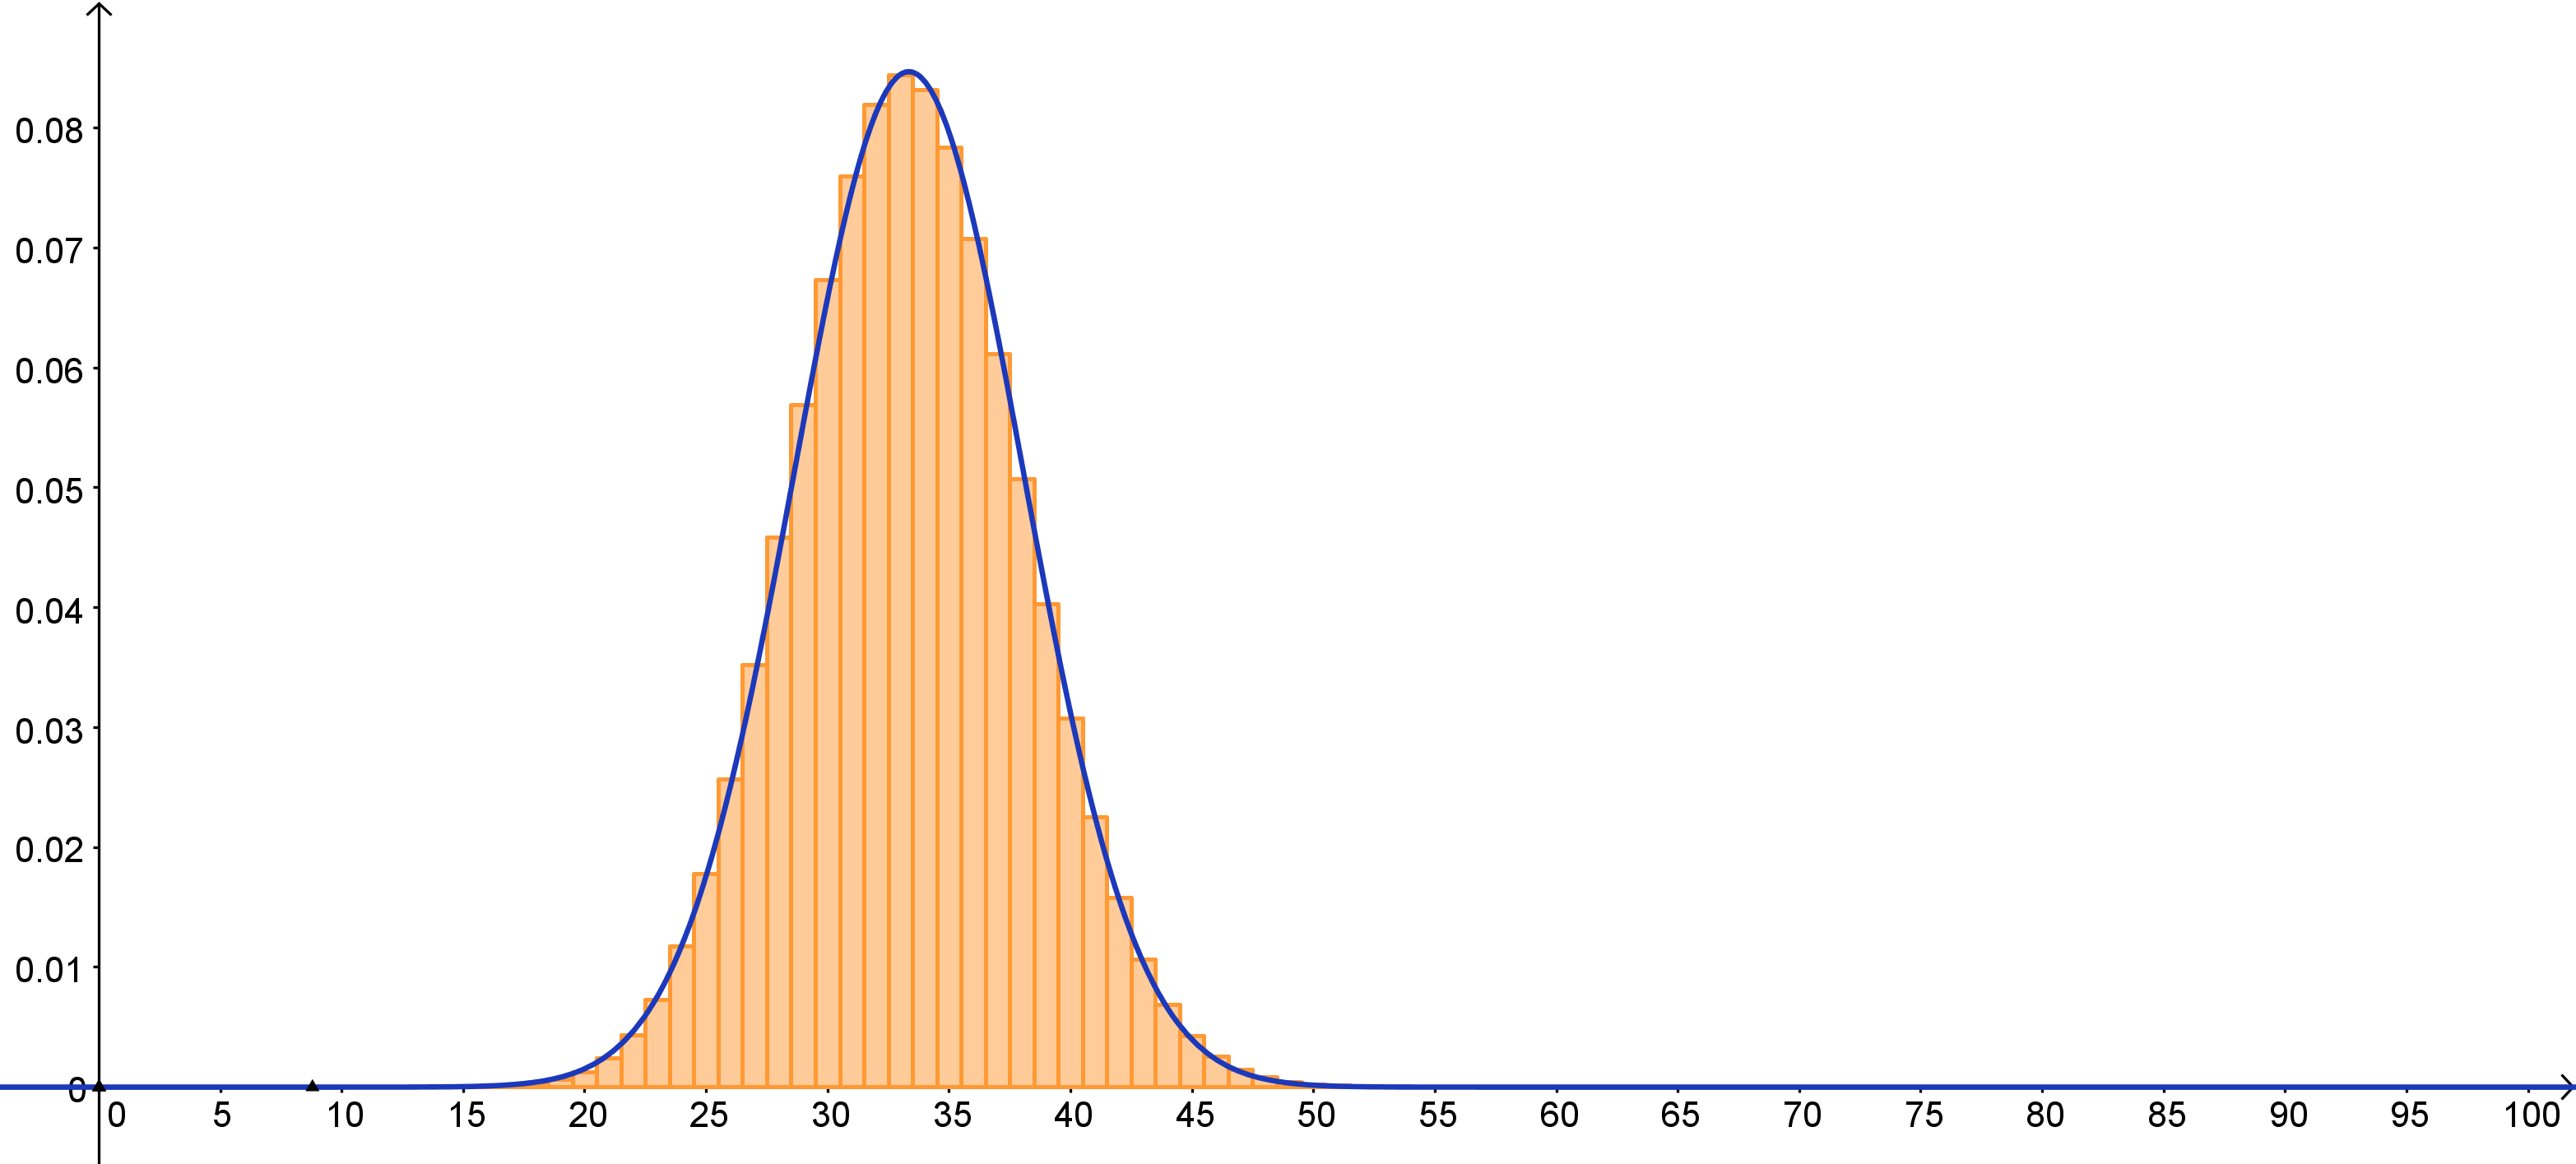
\includegraphics[width=9cm]{../fig/Cap05-HistogramaBinomial03.png}\\
(c)
\end{enColor}
\begin{bn}
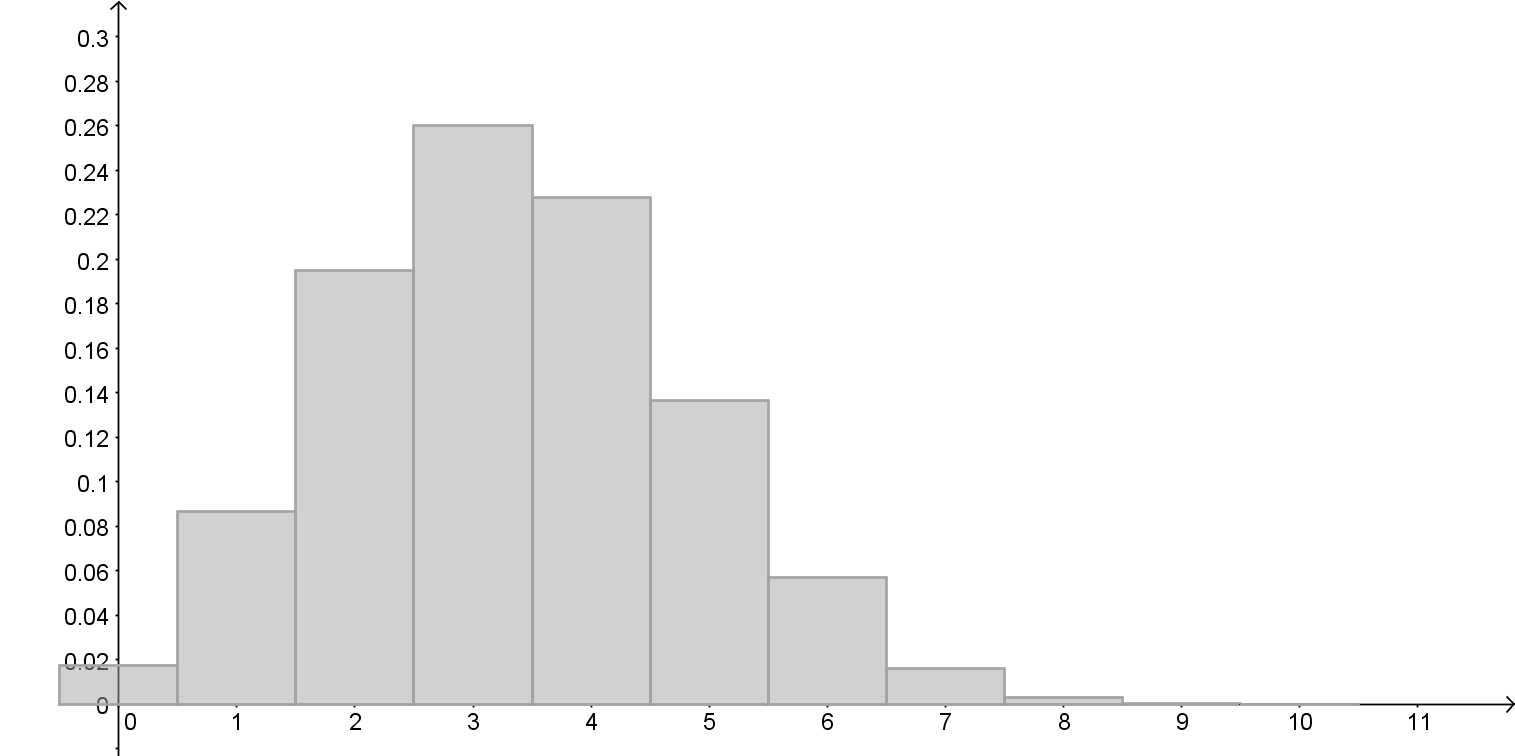
\includegraphics[width=12cm]{../fig/Cap05-HistogramaBinomial01-bn.png}\\
(a)\\
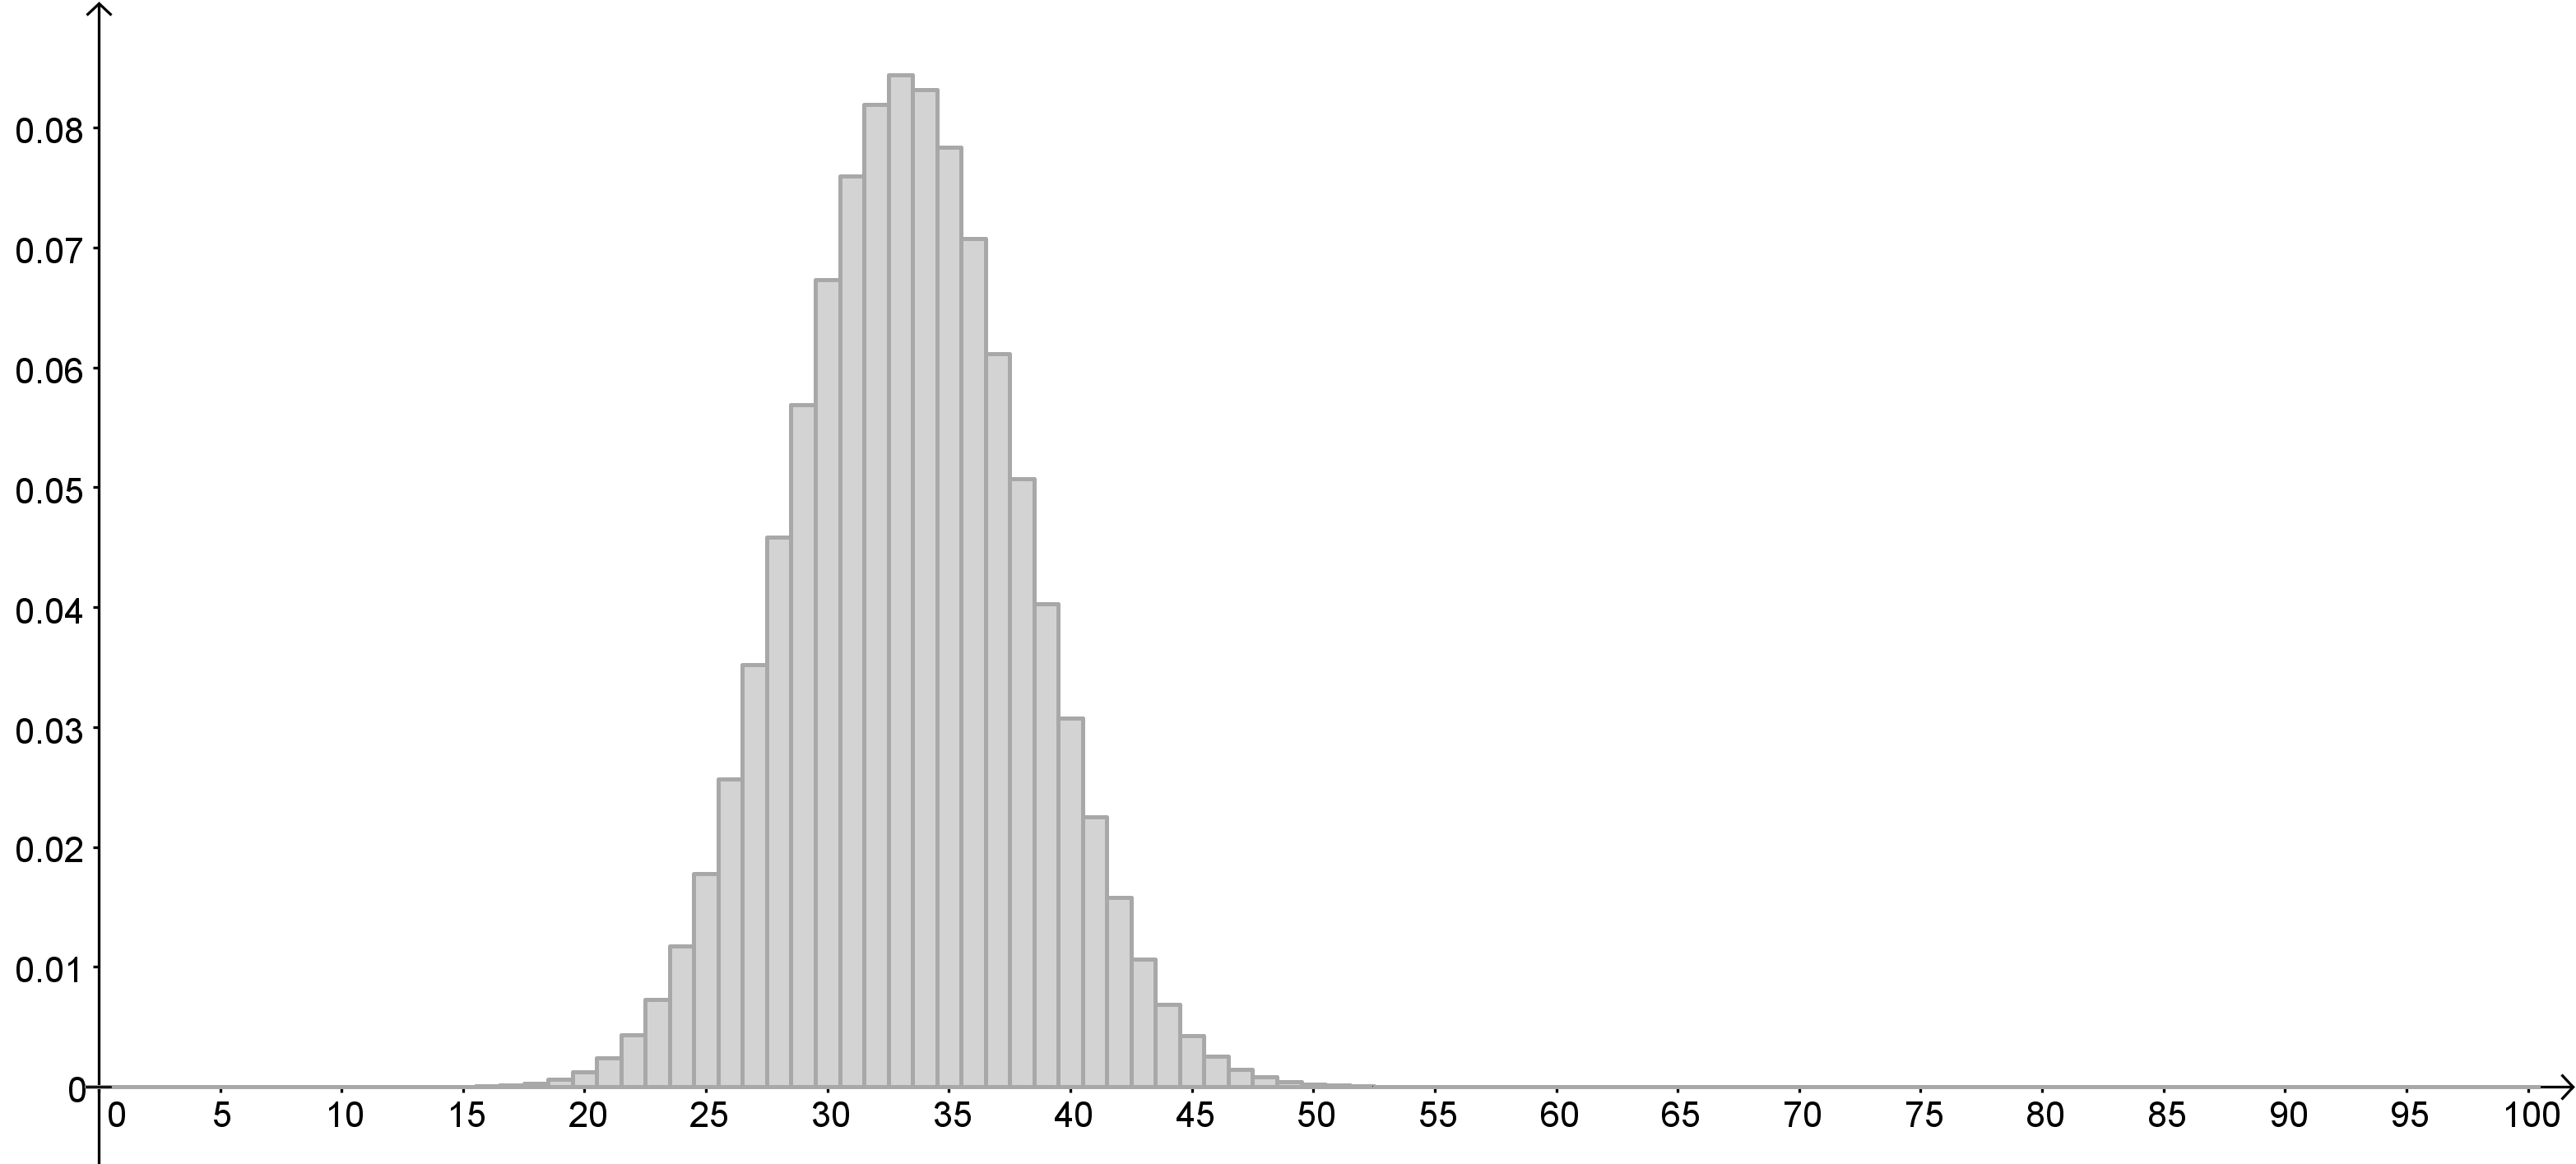
\includegraphics[width=12cm]{../fig/Cap05-HistogramaBinomial02-bn.png}\\
(b)\\
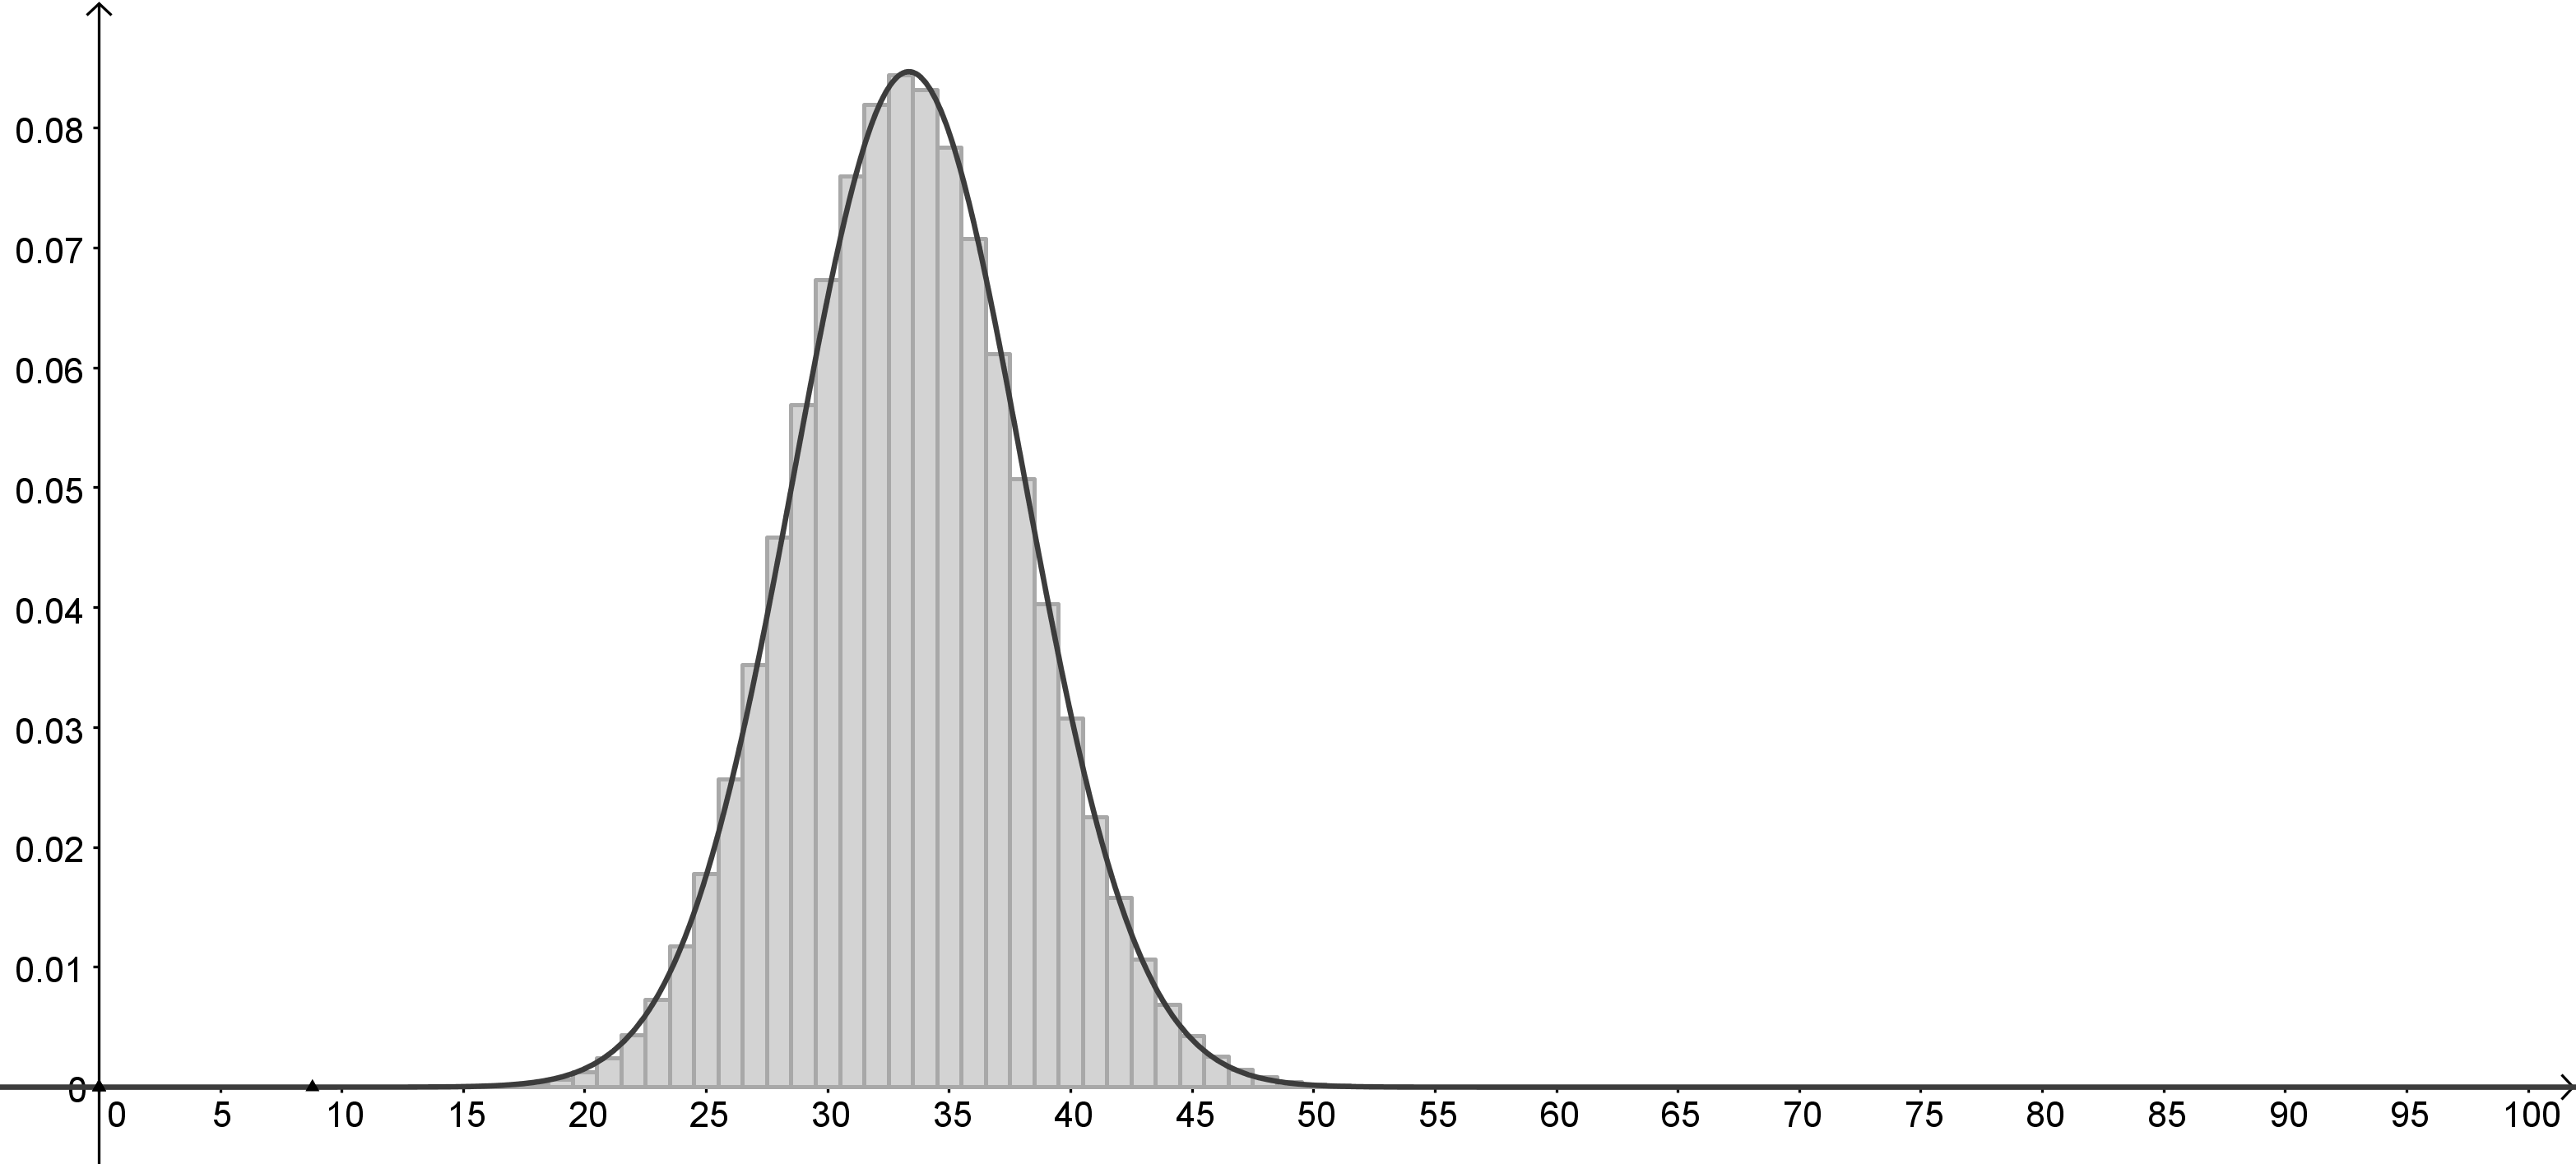
\includegraphics[width=12cm]{../fig/Cap05-HistogramaBinomial03-bn.png}\\
(c)
\end{bn}
\caption{(a) La distribución de probabilidad binomial $B\left(10,\frac{1}{3}\right)$. (b) La distribución de probabilidad binomial $B\left(100,\frac{1}{3}\right)$. (c) La misma distribución $B\left(100,\frac{1}{3}\right)$, con una curva ``misteriosa'' superpuesta.}
\label{cap05:fig:HistogramaBinomial02}
\end{center}
\end{figure}

Atención, de nuevo, a las escalas de esta Figura. En la parte (b) de esta figura la individualidad
de cada uno de los rectángulos empieza a perderse, dando paso a la percepción de una cierta forma
de {\em curva acampanada} que describe lo que ocurre, con una cima en el valor
$\mu_X=\frac{100}{3}$, como se ve en la parte (c) de la Figura
\ref{cap05:fig:HistogramaBinomial02}. ¿Cuál sería esa curva misteriosa, {\em cuál sería su
ecuación}?

Por su proximidad a Newton, estas situaciones en las que tenemos una curva y una aproximación de la
curva mediante rectángulos no le podían resultar extrañas a De Moivre. Esas mismas ideas se estaban
utilizando para sentar las bases del Cálculo Integral. En la Figura
\ref{cap05:fig:FragmentoPrincipiaNewton} hay un fragmento del libro
{\em Principia Mathematica}\index{Principia Mathematica} (páginas 42 y 44; ver el
enlace [\,\ref{enlace0009}\,]\label{enlace0009a}). Nos atrevemos a decir que es uno de
los libros más importantes en la historia de la humanidad, en el que Newton sentó las bases del
Cálculo Diferencial e Integral. En particular, uno de los problemas fundamentales que Newton
abordaba en ese libro era el del cálculo del área bajo la gráfica de una curva, lo que se denomina
la {\sf integral} de la curva. Como puedes ver, en la parte que hemos destacado, Newton sugiere que
se considere un número cada vez mayor de rectángulos bajo la curva (el número de rectángulos tiende
hacia infinito), con bases cada vez más pequeñas, en proporción al total de la figura.
\begin{figure}[bhtp]
\begin{center}
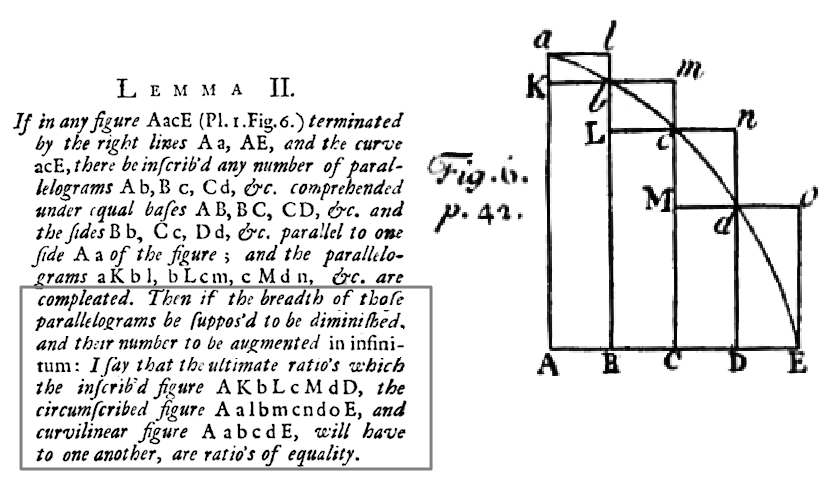
\includegraphics[height=8cm]{../fig/Cap05-NewtonPrincipia.png}
\caption{Un fragmento de los {\em Principia Mathematica} de Newton.}
\label{cap05:fig:FragmentoPrincipiaNewton}
\end{center}
\end{figure}

Esos eran exactamente los ingredientes que aparecían en la situación en la que De Moivre se
encontraba. Así que la pregunta, parecía evidente: {\em ¿cuáles serían esas curvas misteriosas  que
De Moivre estaba empezando a entrever en sus reflexiones sobre la binomial?}  Porque si tuviéramos
la ecuación de esa curva podríamos usarla para aproximar los valores de la binomial sin necesidad
de calcular los molestos números combinatorios. Por otra parte, aquellos matemáticos habían pensado
mucho sobre fórmulas binomiales, así que De Moivre consiguió identificar esas curvas, y vio que las
curvas que buscaba respondían todas a la misma fórmula. Para aproximar una distribución
binomial $B(n,p)$, con $n$ grande, y recordando que $\mu_X=np$ y $\sigma_X=\sqrt{npq}$, había que
usar la curva que ahora llamamos la {\sf curva normal}:

    \begin{center}
    \fcolorbox{black}{Gris025}{
    \begin{minipage}{8cm}
        \begin{center}
        %%%%%%%%%%%%%%%%%%%%%%%%%%%%%%%%%%%%%%%
        {\bf  Ecuación de la curva normal}
        \end{center}
        \index{normal, curva (ecuación)}\index{curva normal}
        %%%%%%%%%%%%%%%%%%%%%%%%%%%%%%%%%%%%%%%
        \begin{equation}\label{cap05:ecu:EcuacionCurvaNormal}
        f_{\mu,\sigma}(x)=\displaystyle\dfrac{1}{\sigma\sqrt{2\pi}}e^{-\frac{1}{2}\left(\frac{x-\mu}{\sigma}\right)^2}
        \quad\\[2mm]
        \end{equation}
        %%%%%%%%%%%%%%%%%%%%%%%%%%%%%%%%%%%%%%%
    \end{minipage}
    }
    \end{center}
{!`}En efecto, esos son el número $e$ y el número $\pi$! Produce un cierto vértigo verlos aparecer aquí, cuando todo esto ha empezado lanzando dados... Veamos como funciona esta fórmula en un ejemplo.
    \begin{Ejemplo}
    \label{ejem:BinomialVsNormal}
    Volvamos al cálculo que proponíamos al principio de esta sección. Calculemos $P(X=30)$ para una distribución binomial $B(100,1/3)$ (es decir, que puedes pensar que estamos tirando un dado 100 veces y preguntándonos por la probabilidad de obtener 30 veces un número 1 o 2. Probabilidad $2/6=1/3$). Si usamos la definición, calcularíamos
   \[\displaystyle
   P(X=k)=\binom{n}{k}\cdot p^k\cdot q^{n-k},
   \]
   con $n=100, k=30, p=\frac{1}{3}$. Para calcular esto hay que obtener $\binom{100}{30}\approx 2.9372\cdot 10^{25}$. Con esto, finalmente se obtiene $P(X=30)\approx 0.06728$. Si usamos la función $f_{\mu,\sigma}(x)$ con $\mu=np=\frac{100}{3}$ y $\sigma=\sqrt{n\cdot p\cdot q}\approx4.714$ se obtiene
   \[f_{\mu,\sigma}(30)\approx 0.06591.\]
   La aproximación, como vemos, no está mal, {\em aunque no es espectacular}. Hay un detalle que podría mejorarla, pero lo dejamos para más adelante, cuando hayamos entendido esto mejor.
   \quad\qed
   \end{Ejemplo}
%    Antes de seguir adelante, en \textattachfile{AproximacionBinomialPorNorrmal.R}{\textcolor{blue}{este fichero}} tienes las instrucciones en R para repetir esos cálculos.

\section{Las distribuciones continuas entran en escena...} \label{sec:distribucionesContinuasEntranEscena}

Por otra parte, regresamos a una idea que ya vislumbramos en el Capítulo \ref{cap:IntroduccionEstadisticaDescriptiva}, al hablar de datos agrupados por intervalos. Allí vimos que, al tratar con algunos conjuntos de datos,  si pensamos en valores de $n$ cada vez más grandes, las preguntas como $P(X=k)$ se vuelven cada vez menos relevantes. Si vas a lanzar un dado 10000 veces, la probabilidad de obtener exactamente $30$ veces 1 o 2 es prácticamente nula. Puedes usar el ordenador para calcularlo, como veremos en el Tutorial05. En resultado es del orden de $10^{-128}$, inimaginablemente pequeño. Incluso los valores más probables (cercanos a la media $\mu$) tienen en este ejemplo  probabilidades de en torno a $0.2$ (o un $2\%$).  No, en casos como este, lo que tiene interés es preguntar por {\em intervalos de valores}. igual que hacíamos en la Estadística Descriptiva. Es decir, nos preguntamos ¿cuál es la probabilidad de obtener 300 éxitos o menos? O también, ¿cuál es la probabilidad de obtener entre 300 y 600 éxitos del total de 1000? Para entender la respuesta, veamos algunos ejemplos.

\begin{ejemplo}
\label{cap05:ejem:DistribucionBinomialProbabilidadIntervalo01}
Volvamos por un momento a un valor de $n$ más moderado. Por ejemplo $n=21$, todavía con $p=1/3$. La media es $\mu=7$, y el diagrama correspondiente a la distribución $B(21,1/3)$ aparece en la Figura \ref{cap05:fig:HistogramaBinomial04}.
\begin{figure}[ht]
\begin{center}
\begin{enColor}
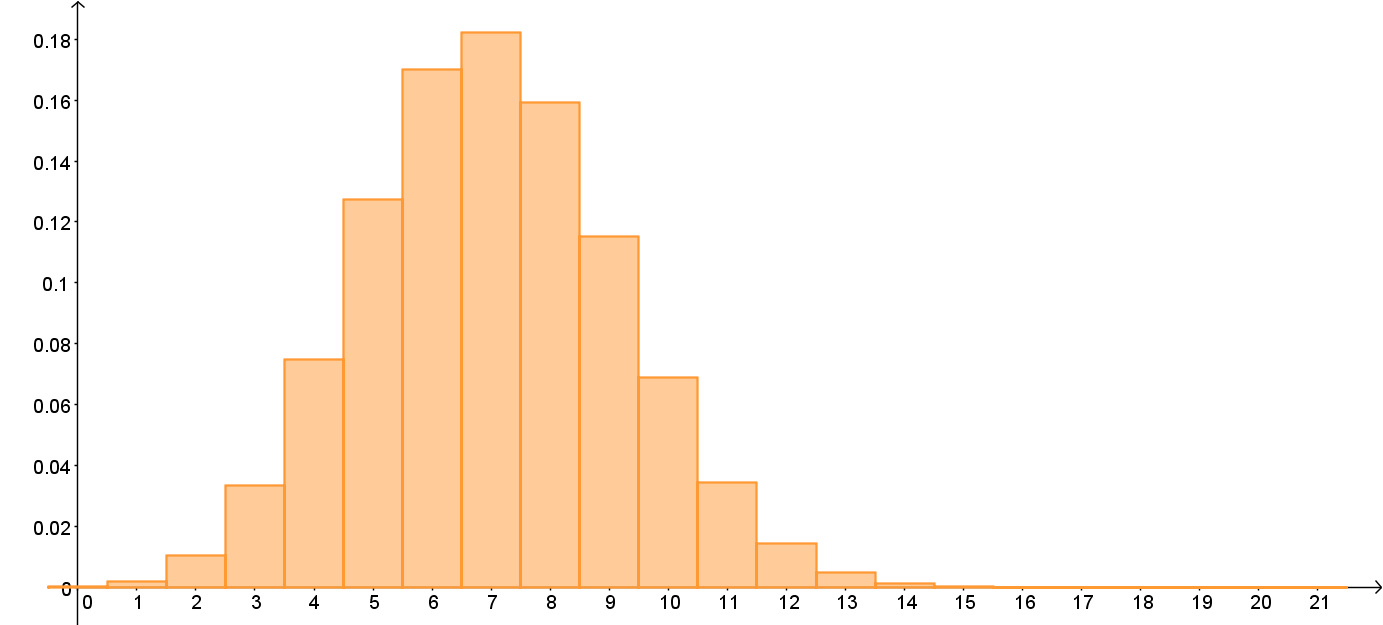
\includegraphics[width=12cm]{../fig/Cap05-HistogramaBinomial04.png}
\end{enColor}
\begin{bn}
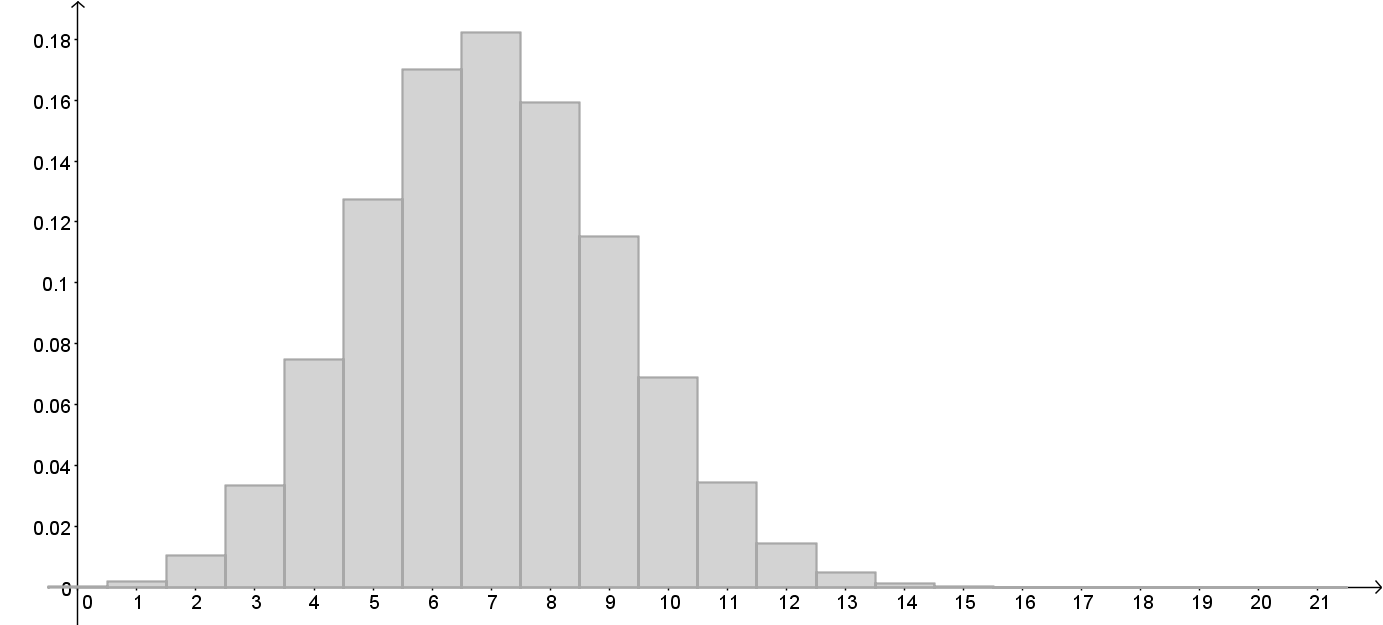
\includegraphics[width=12cm]{../fig/Cap05-HistogramaBinomial04-bn.png}
\end{bn}
\caption{Distribución binomial $n=21$, $p=\frac{1}{3}$.}
\label{cap05:fig:HistogramaBinomial04}
\end{center}
\end{figure}
¿Cuál es la probabilidad de obtener entre 5 y 9 éxitos (ambos inclusive)? Pues la suma de áreas de los rectángulos oscuros de la Figura \ref{cap05:fig:HistogramaBinomial05} (recuerda que la suma total de áreas de los rectángulos es 1).
\begin{figure}[ht]
\begin{center}
\begin{enColor}
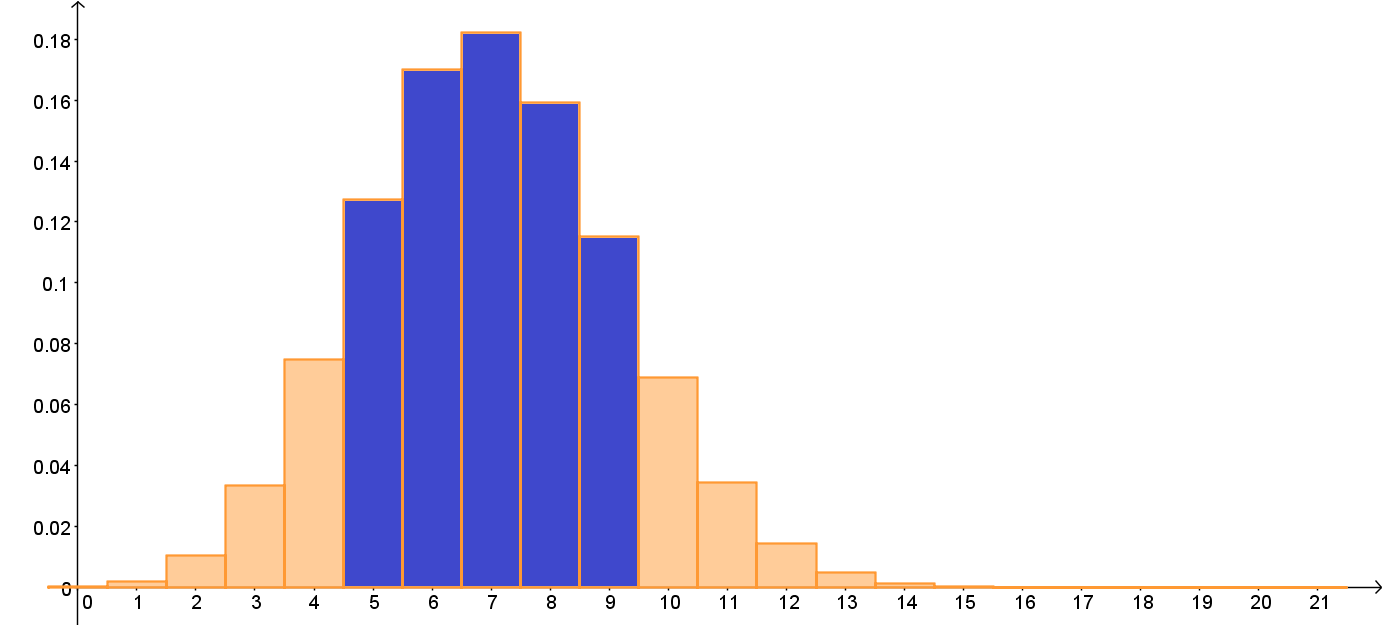
\includegraphics[width=12cm]{../fig/Cap05-HistogramaBinomial05.png}
\end{enColor}
\begin{bn}
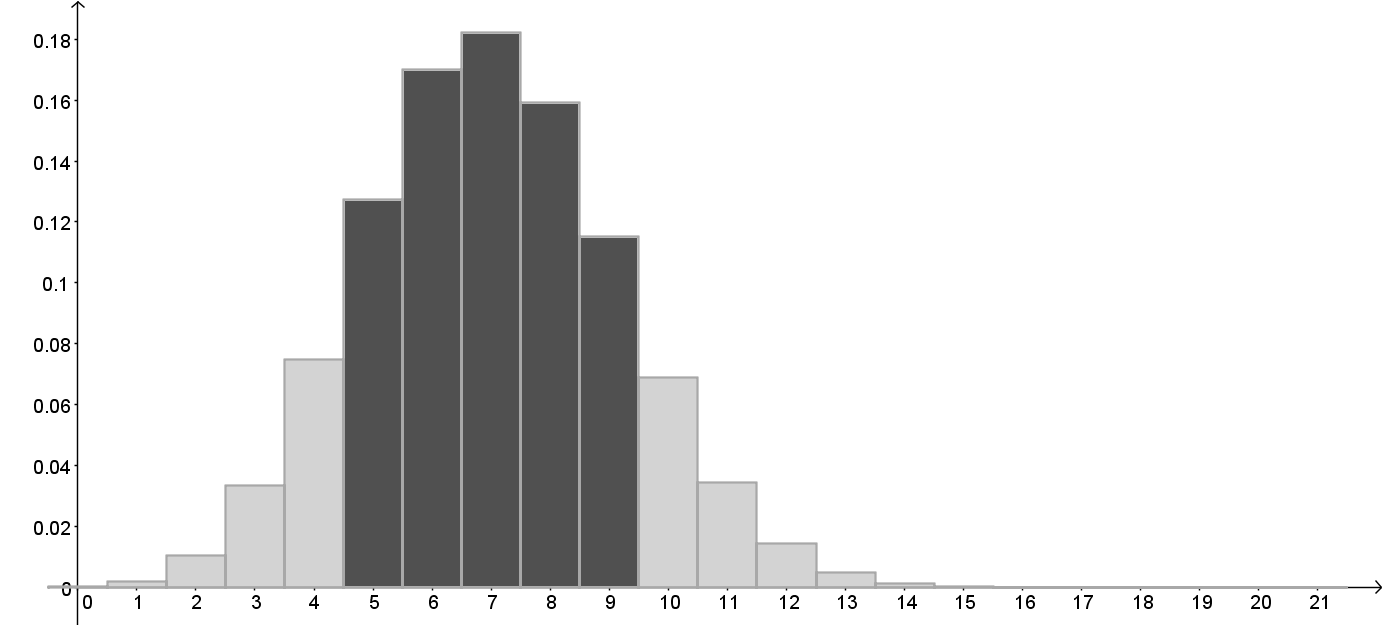
\includegraphics[width=12cm]{../fig/Cap05-HistogramaBinomial05-bn.png}
\end{bn}
\caption{Probabilidad $P(5\leq X\leq 9)$ en la Distribución Binomial $B\left(21,\frac{1}{3}\right)$.}
\label{cap05:fig:HistogramaBinomial05}
\end{center}
\end{figure}
Ese valor es
\[P(5\leq X\leq 9)=P(X=5)+P(X=6)+\cdots+P(X=9),\]
y es aproximadamente $0.75$ (lo veremos en el Tutorial05). Si ahora volvemos al problema para $B(1000,1/3)$  y nos preguntamos por $P(300\leq X\leq 600)$, vemos que tendríamos que sumar el área de 301 rectángulos para calcular esa probabilidad. ¿No hay una forma mejor de hacer esto?
\qed
\end{ejemplo}

Para De Moivre, en contacto con las ideas recién nacidas sobre cálculo integral y su aplicación al cálculo del área bajo una curva, la respuesta tuvo que ser evidente. Porque precisamente Newton había descubierto que, para definir el área bajo la gráfica de una función, para valores de $x$ entre $a$ y $b$, había que considerar una aproximación del área mediante $n$ rectángulos y estudiar el límite de esas aproximaciones para $n$ cada vez más grande, como se ilustra en la Figura \ref{cap05:fig:IntegralRectangulosSumaInferior}. Para concretar, la notación (que puede intimidar un poco al principio) es esta: el área bajo la gráfica de la función\index{área bajo la gráfica de una función} $f$ en el intervalo $(a,b)$ se representa con el símbolo
\[\int_a^b f(x)dx.\]
Este símbolo se lee {\em la integral de $f$ en el intervalo $(a,b)$\index{integral de una función en un intervalo}.} No podemos, ni queremos, convertir este curso en un curso de Cálculo Integral, pero si queremos aprovechar la ocasión para que el lector\footnote{Especialmente el lector que no tiene experiencia con integrales o que sí la tiene, y ha desarrollado una cierta alergia al concepto.} tenga la oportunidad de ver, sin formalismo pero con algo de detalle, la relación que existe entre el cálculo de probabilidades de la binomial y el Cálculo Integral, porque es un ejemplo de las razones (a veces inesperadas) que hacen que los matemáticos consideren tan importante el problema de calcular áreas.
\begin{figure}[hp]
\begin{center}
\begin{enColor}
(a)\\
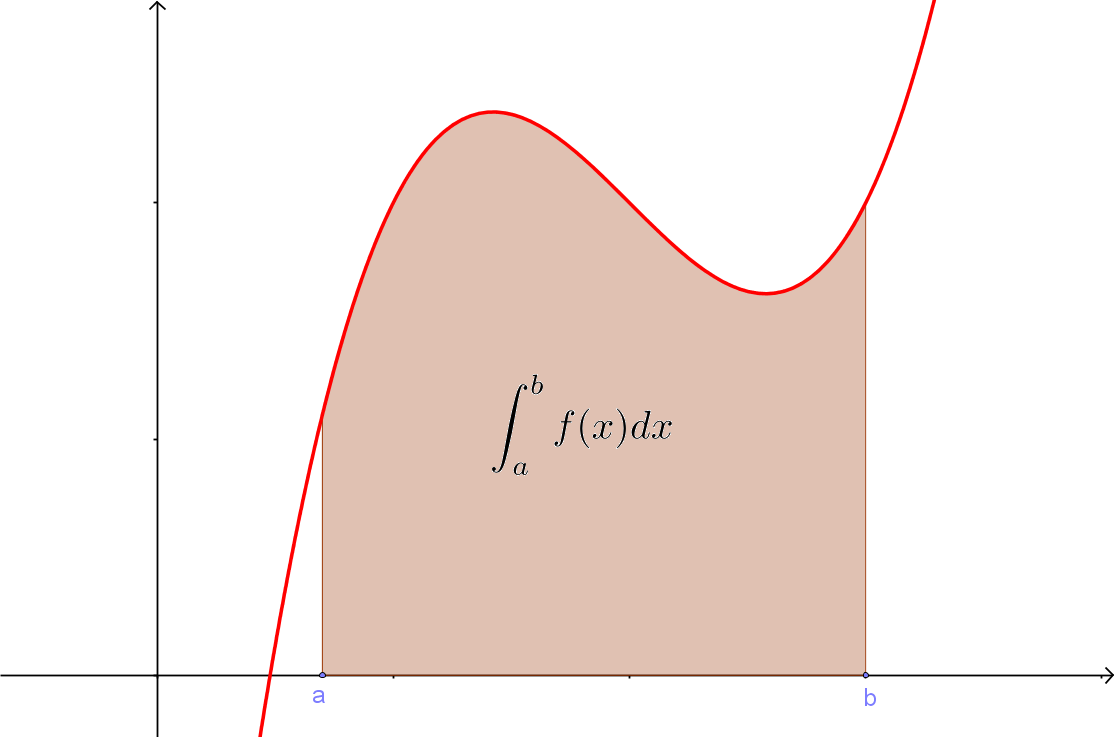
\includegraphics[width=12cm]{../fig/Cap05-IntegralRectangulosSumaInferior.png}\\
(b)\\
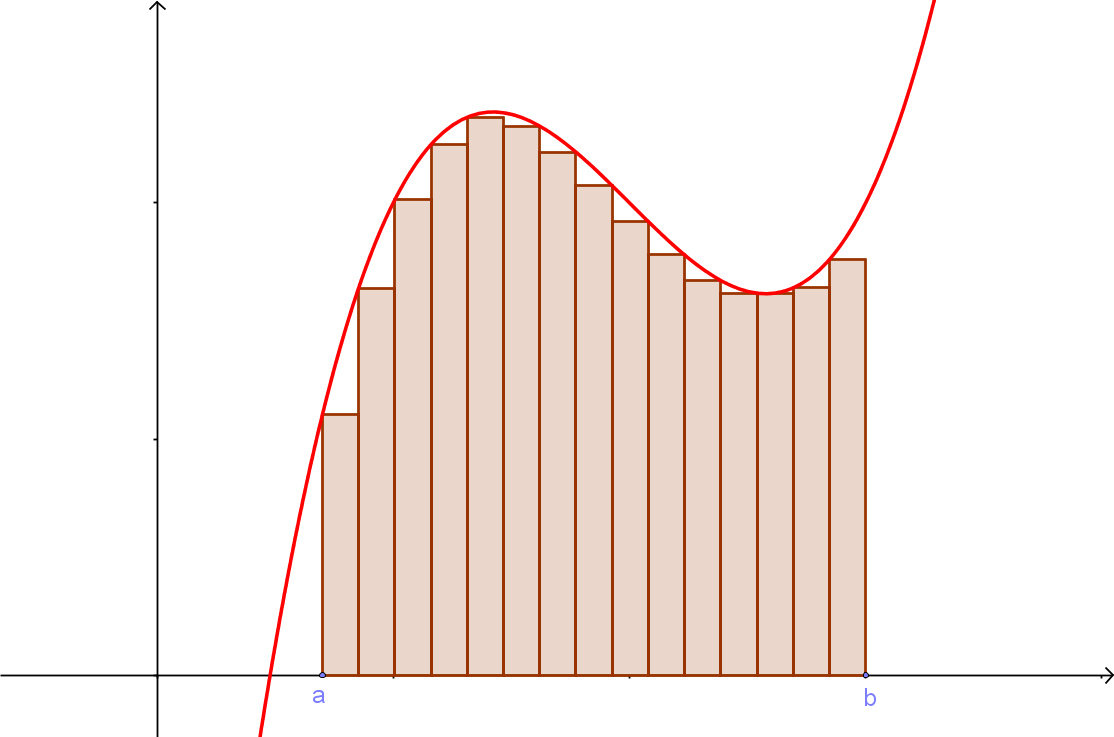
\includegraphics[width=12cm]{../fig/Cap05-IntegralRectangulosSumaInferior-a.png}
\end{enColor}
\begin{bn}
(a)\\
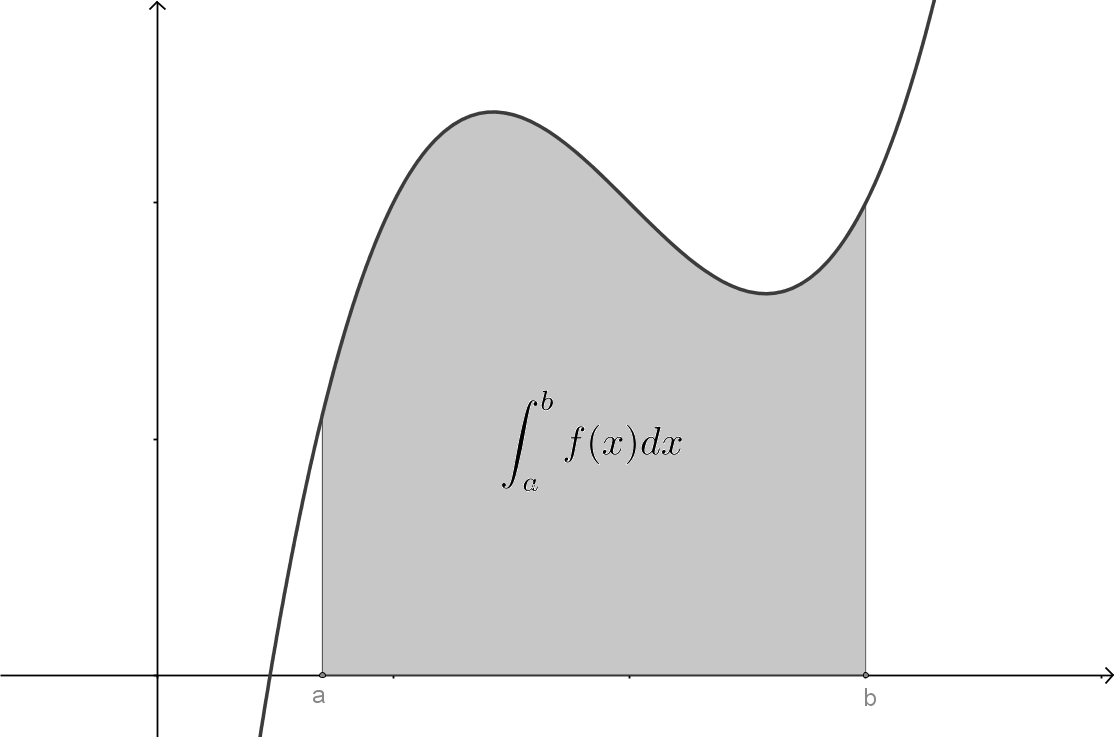
\includegraphics[width=12cm]{../fig/Cap05-IntegralRectangulosSumaInferior-bn.png}\\
(b)\\
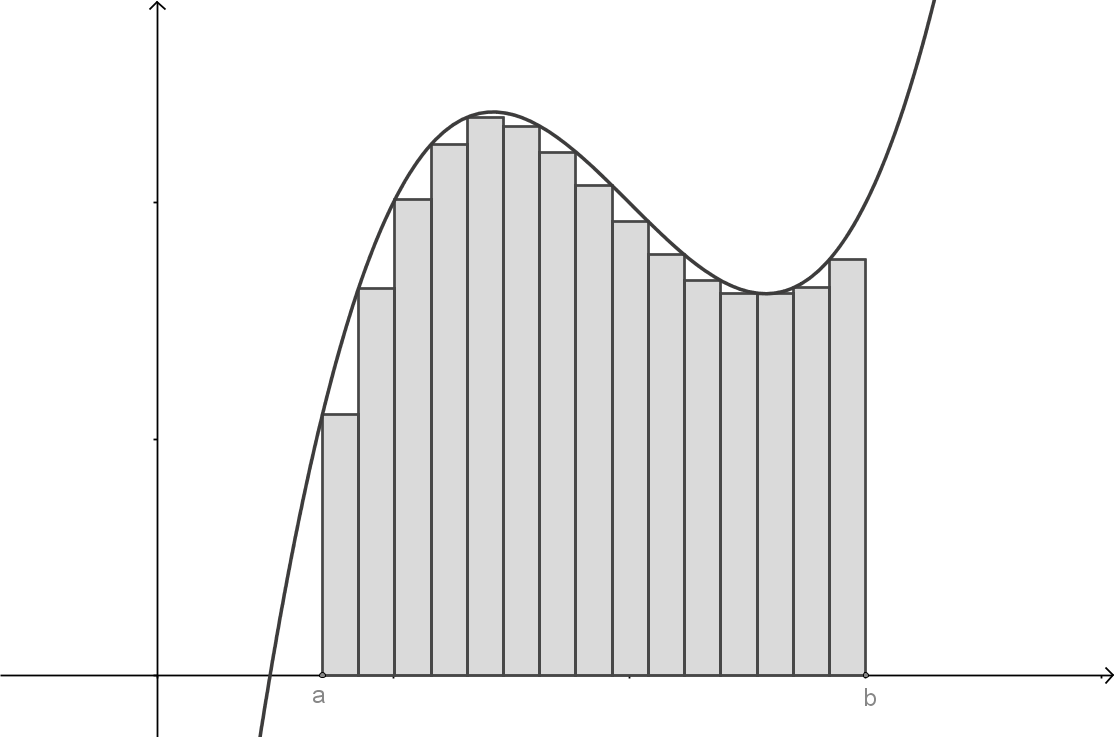
\includegraphics[width=12cm]{../fig/Cap05-IntegralRectangulosSumaInferior-a-bn.png}
\end{bn}
\caption{Newton mostró como relacionar (a) el área bajo una curva (una integral) con (b) una suma de áreas de rectángulos cada vez más numerosos y estrechos.}
\label{cap05:fig:IntegralRectangulosSumaInferior}
\end{center}
\end{figure}
Y para perderle un poco el miedo al símbolo, vamos a pensar desde el lado que nos resulta más familiar, el de la suma de áreas de rectángulos. El área de un rectángulo es, naturalmente,
\[\mbox{altura}\cdot\mbox{base}.\]
Así que la suma de las áreas de los rectángulos entre $a$ y $b$ se puede escribir:
\[\sum_{\mbox{desde $a$}}^{\mbox{hasta $b$}}\left(\mbox{alturas}\cdot\mbox{bases}\right)\]
La letra griega sigma mayúscula $\displaystyle\Sigma$ que usamos en el sumatorio es el equivalente de la letra latina $S$, y se usa para representar una $\Sigma$uma. Pero si sustituyes la S griega por una S latina alargada, como este símbolo $\displaystyle\int$, verás que tienes:
\[\int_{\mbox{desde $a$}}^{\mbox{hasta $b$}}\left(\mbox{alturas}\cdot\mbox{bases}\right)\]
Y lo único que se necesita ahora es darse cuenta de que la altura de los rectángulos depende de la función $f(x)$ que estamos integrando, y el símbolo $dx$ representa la  base de esos rectángulos. Así que el símbolo de la integral tiene esta interpretación:
\[
\begin{array}{ccc}
\underbrace{\quad\int_a^b\quad}_{\mbox{\small Suma de $a$ a $b$}}&
\raisebox{-2mm}{$\underbrace{\vspace{2mm}\quad f(x)\quad}_{\mbox{\small alturas }}$}&
\raisebox{-3mm}{$\underbrace{\vspace{2mm}\quad dx\quad}_{\mbox{\small bases. }}$}
\end{array}
\]
Y animamos al lector a que recuerde siempre que, por complicada que pueda parecer, una integral está relacionada con algo sencillo, como una suma de áreas de rectángulos. La relación, más precisamente, consiste en que a medida que consideramos un número mayor de rectángulos, con bases cada vez más estrechas, las dos cantidades se van pareciendo cada vez más. En el Tutorial05 usaremos el ordenador para ilustrar de forma dinámica estas ideas.

\begin{ejemplo}
\label{cap05:ejem:DistribucionBinomialProbabilidadIntervalo02}
Vamos a volver, equipados con estas ideas, al  problema de calcular la probabilidad $P(300\leq X\leq 600)$\label{cap05:lugar:DiscusionAproximarBinomialNormal} para la distribución binomial $B(1000,1/3)$. Lo que vamos a hacer es usar
$f_{\mu,\sigma}(x)=f_{1000,1/3}(x)$, que es la curva normal que aproxima a $B(1000,1/3)$. Usando esta función, podemos aproximar la probabilidad mediante esta integral:
\[\int_{300}^{600}f_{1000,1/3}(x)dx\]
No entramos aquí en los detalles de cómo calcularla, pero el resultado es aproximadamente $0.9868$. Para comparar, y aprovechando que tenemos la suerte de disponer de ordenadores (que, por el momento, no protestan ante tareas como esta), le hemos pedido a un programa de ordenador que calcule el valor exacto, es decir que calcule:
\[P(X=300)+P(X=301)+\cdots+P(X=600).\]
usando los números combinatorios. Es decir, que calcule:
\[\sum_{k=300}^{600}\binom{1000}{k}\cdot\left(\dfrac{1}{3}\right)^k\cdot\left(\dfrac{2}{3}\right)^{1000-k}.\]
La fracción que se obtiene es, nada menos, esta:\\
$(5\-\-3\-8\-0\-1\-2\-9\-5\-1\-2\-3\-0\-2\-9\-7\-0\-7\-9\-2\-3\-4\-2\-8\-6\-0\-3\-1\-4\-3\-9\-8\-0\-7\-6\-0\-9\-3\-2\-6\-0\-9\-8\-3\-6\-6\-1\-7\-5\-4\-7\-1\-6\-8\-1\-2\-5\-3\-5\-4\-1\-9\-3\-2\-0\-3\-8\-4\-1\-7\-6\-3\-4\-3\-6\-0\-9\-4\-7\-7\-2\-3\-0\-0\-9\-6\-9\-0\-5\-5\-1\-4\-0\-4\-9\-9\-5\-2\-2\-8\-8\-0\-1\-2\-2\-1\-2\-0\-1\-5\-5\-7\-5\-6\-3\-4\-7\-8\-0\-5\-7\-2\-2\-2\-7\-0\-8\-6\-6\-8\-1\-7\-4\-7\-1\-9\-2\-2\-1\-7\-7\-0\-2\-3\-8\-4\-1\-3\-8\-8\-8\-3\-4\-0\-7\-8\-8\-6\-2\-8\-1\-8\-3\-0\-5\-2\-9\-2\-8\-2\-7\-1\-8\-9\-1\-1\-9\-1\-0\-7\-1\-0\-3\-1\-7\-8\-3\-5\-9\-3\-1\-8\-2\-6\-3\-5\-0\-4\-4\-5\-6\-0\-7\-9\-4\-2\-8\-0\-5\-1\-2\-0\-2\-5\-4\-2\-8\-7\-1\-0\-0\-5\-7\-5\-2\-0\-7\-1\-9\-0\-1\-3\-0\-2\-6\-1\-6\-3\-0\-4\-5\-3\-2\-3\-4\-7\-9\-3\-6\-4\-3\-7\-3\-1\-2\-0\-4\-3\-9\-8\-7\-4\-9\-3\-0\-2\-8\-2\-2\-0\-5\-9\-6\-4\-5\-2\-4\-8\-7\-8\-1\-9\-5\-3\-0\-9\-7\-6\-6\-6\-4\-1\-5\-5\-8\-1\-3\-2\-8\-3\-8\-9\-6\-1\-9\-2\-4\-4\-4\-6\-6\-9\-9\-7\-0\-9\-9\-1\-6\-0\-0\-5\-0\-9\-1\-8\-4\-4\-2\-4\-4\-2\-9\-9\-4\-7\-0\-9\-6\-4\-6\-5\-3\-6\-9\-4\-6\-8\-5\-5\-0\-6\-9\-4\-7\-5\-8\-8\-7\-0\-9\-1\-2\-5\-0\-1\-2\-6\-1\-0\-3\-8\-1\-7\-6\-2\-8\-8\-8\-7\-4\-2\-2\-3\-8\-3\-8\-2\-3\-3\-5\-6\-3\-6\-4\-7\-3\-4\-9\-0\-0\-0\-4\-2\-5\-9\-7\-7\-7\-7\-8\-8\-4\-7\-3\-4\-4\-5\-4\-3\-9\-1\-7\-7\-7\-9\-7\-7\-7\-0\-6\-6\-6\-9\-8\-3\-1\-9\-3\-4\-5\-5\-5\-1\-3\-1\-0\-9\-7\-6\-9\-6\-7\-9\-6\-1\-8\-7\-4\-8\-7\-8\-4\-3\-3\-7\-1\-2\-3\-4\-3\-6\-1\-3\-4\-4\-)\,/\,(5\-4\-4\-0\-6\-2\-0\-6\-5\-6\-2\-9\-9\-6\-1\-5\-7\-8\-9\-6\-7\-2\-6\-5\-5\-3\-8\-9\-9\-2\-6\-5\-2\-0\-0\-2\-4\-5\-4\-9\-0\-6\-1\-8\-6\-3\-1\-7\-7\-5\-6\-4\-4\-7\-5\-9\-8\-7\-3\-2\-6\-6\-1\-8\-2\-1\-7\-4\-0\-1\-6\-3\-5\-1\-7\-1\-6\-2\-5\-1\-0\-0\-9\-9\-0\-8\-5\-7\-2\-5\-8\-6\-4\-4\-4\-7\-7\-6\-2\-1\-2\-5\-0\-6\-5\-7\-5\-2\-1\-3\-8\-6\-3\-0\-6\-9\-2\-3\-2\-7\-5\-5\-1\-8\-3\-3\-1\-6\-1\-3\-5\-8\-2\-7\-9\-3\-8\-7\-5\-9\-8\-9\-0\-6\-4\-7\-1\-2\-9\-9\-5\-6\-9\-4\-1\-3\-1\-8\-0\-0\-9\-0\-6\-2\-7\-6\-5\-3\-6\-2\-9\-9\-6\-0\-4\-4\-3\-6\-2\-7\-4\-7\-9\-1\-0\-6\-5\-6\-9\-8\-9\-3\-5\-2\-8\-5\-5\-5\-7\-2\-0\-2\-1\-2\-9\-9\-9\-4\-3\-1\-2\-9\-2\-6\-4\-5\-6\-5\-7\-5\-3\-7\-2\-9\-3\-4\-5\-4\-5\-0\-1\-2\-5\-9\-9\-0\-3\-7\-7\-4\-9\-1\-9\-3\-7\-7\-2\-3\-2\-3\-0\-0\-6\-1\-9\-8\-2\-6\-3\-8\-9\-0\-8\-6\-5\-6\-1\-4\-8\-3\-7\-6\-4\-2\-1\-9\-9\-1\-6\-4\-7\-6\-9\-1\-1\-8\-5\-9\-0\-3\-9\-2\-4\-6\-1\-9\-5\-4\-3\-8\-7\-3\-9\-1\-8\-5\-5\-2\-6\-8\-5\-9\-4\-9\-1\-2\-6\-6\-9\-0\-6\-2\-9\-2\-2\-7\-5\-0\-6\-8\-4\-7\-6\-6\-6\-9\-9\-1\-2\-7\-1\-4\-7\-8\-1\-2\-9\-8\-9\-3\-1\-7\-2\-2\-1\-8\-0\-6\-3\-2\-7\-6\-1\-0\-5\-8\-9\-4\-7\-3\-9\-5\-8\-2\-1\-5\-4\-7\-2\-9\-9\-8\-7\-4\-6\-9\-8\-2\-5\-7\-2\-0\-9\-4\-4\-0\-5\-7\-1\-2\-3\-8\-2\-9\-6\-4\-7\-1\-6\-4\-1\-8\-4\-0\-0\-9\-8\-2\-9\-7\-9\-8\-4\-6\-9\-7\-2\-6\-3\-5\-3\-3\-1\-8\-8\-7\-8\-4\-8\-4\-1\-9\-0\-6\-1\-7\-7\-2\-0\-7\-5\-5\-8\-0\-7\-9\-0\-8\-3\-5\-8\-1\-3\-8\-6\-3\-7\-9\-7\-7\-5\-8\-1\-0\-7\-)$ \\
que es aproximadamente $0.9889$ (con cuatro cifras significativas).
\qed
\end{ejemplo}
Hemos incluido la fracción completa (que es reducida, sin factores comunes a numerador y denominador) para que el lector tenga ocasión de ponderar la situación pausadamente. Es cierto, sobre todo para alguien que comienza el estudio de la Estadística, que cambiar una suma por una integral puede parecer una complicación innecesaria. {!`}Pero, como demuestra esa fracción, no hablamos de una suma cualquiera! El esfuerzo computacional que supone hallar esa fracción es muy superior al de calcular el valor de la integral, de manera que, hasta hace muy pocos años, era imposible, en la práctica, obtener ese valor exacto. Insistimos, porque creemos que es esencial que se entienda esto: frente al cálculo directo de los valores de la Binomial, {\em la integral de la curva normal es un atajo, es el cámino más cómodo}. Y si se tiene en cuenta que el valor exacto es $0.9889$, y que la aproximación de la curva normal es $0.9868$, el atajo funciona bastante bien (sobre todo, desde la perspectiva previa a los ordenadores).

%De hecho, si usamos R para sumar los valores $P(X=300)+\cdots+P(X=600)$ se obtiene aproximadamente $0.9888$. La aproximación está muy bien, y eso que aún tenemos pendiente mejorar el ajuste de la curva $f_{\mu,\sigma}(x)$ con los valores de $B(p,n)$.

Recapitulemos: para calcular la probabilidad $P(a\leq X\leq b)$ de $B(n,p)$ hemos usado una cierta función $f_{\mu,\sigma}(x)$, y hemos visto que
    \[P(a\leq X\leq b)\approx \int_a^b f_{\mu,\sigma}(x)dx.\]
Las ideas que subyacen a la aproximación de la Distribución Binomial por la normal son muy importantes; de hecho, son en algún sentido uno de los hallazgos más importante de toda la historia de la Estadística (y, sin temor a exagerar, de toda la historia de la Ciencia). Pero no es la única aproximación de ese estilo que encontraron los matemáticos. Y a medida que se acostumbraban a estas ideas, y empezaban a pensar en el lado derecho de esa aproximación, se dieron cuenta de que esas integrales constituían, por si mismas, una forma de repartir o {\em distribuir} la probabilidad, muy similar a lo que hemos aprendido a hacer con las tablas de las variables aleatorias discretas (como la Tabla \ref{cap04:tabla:tablaDensidadProbabilidadGenericaVariableAleatoriaDiscreta}, pág. \pageref{cap04:tabla:tablaDensidadProbabilidadGenericaVariableAleatoriaDiscreta}). Sólo que aquí, a diferencia de lo que ocurre en esas Tablas, no hay una {\em lista discreta} de valores, sino un {\em intervalo continuo}. La palabra clave aquí es {\em continuo}. De hecho, hemos dejado pendiente desde la Sección \ref{sec:variablesAletorias} (pág. \pageref{sec:variablesAletorias}) el tratamiento general de las variables aleatorias continuas. En el próximo apartado retomamos esa discusión, a la luz de lo que hemos aprendido. Cuando hayamos profundizado en esto, y hayamos extendido nuestro vocabulario, volveremos al tema de la aproximación de la Distribución Binomial.

\section{Función de densidad, media y varianza de una variable continua.}
\label{cap05:sec:MasDetallesSobreDistribucionesContinuas}

La idea con la que hemos cerrado el apartado anterior es que se puede usar una integral para asignar valores de probabilidad. En esta sección vamos a ver cómo se hace esto con, inevitablemente, bastantes más detalles técnicos. Pero tratando, como siempre, de no enredarnos en el formalismo y apoyarnos en el ordenador todo lo que nos sea posible. No te asustes si nunca has calculado una integral. El ordenador calculará por nosotros. Tampoco calculamos ``a mano'' nunca un logaritmo (salvo los más elementales), y nos hemos acostumbrado a que las máquinas se encarguen de esa tarea. Naturalmente, cuanto más aprendas sobre las {\em propiedades} de las integrales, tanto mejor. Pero queremos distinguir entre las propiedades y el cálculo, porque son cosas distintas (como sucede, de nuevo, en el caso de los logaritmos).

Como hemos dicho al cerrar la anterior sección, en una variable discreta, que toma una cantidad
finita de valores, utilizamos  una tabla como la Tabla
\ref{cap04:tabla:tablaDensidadProbabilidadGenericaVariableAleatoriaDiscreta}, pág.
\pageref{cap04:tabla:tablaDensidadProbabilidadGenericaVariableAleatoriaDiscreta}) para repartir la
probabilidad entre los distintos valores. Pero con una variable aleatoria, que toma infinitos
valores (todos los valores de un intervalo), no podemos hacer eso. Si la variable aleatoria
continua $X$ toma todos los valores del intervalo $(a,b)$, vamos a aprender a utilizar las
integrales, para repartir la probabilidad entre esos valores. En el siguiente cuadro se resume la
información esencial, que a continuación vamos a explorar con detenimiento.
    \begin{center}
    \fcolorbox{black}{Gris025}{
    \begin{minipage}{12cm}
        \begin{center}
        %%%%%%%%%%%%%%%%%%%%%%%%%%%%%%%%%%%%%%%
        {\bf  Función de densidad de una variable aleatoria continua}
        \end{center}
        \index{variable aleatoria continua y su función de densidad}
        %%%%%%%%%%%%%%%%%%%%%%%%%%%%%%%%%%%%%%%
        Para definir una variable aleatoria continua $X$, que tome valores en $(-\infty,\infty)$  podemos utilizar una {\sf función de densidad}, que es una función $f(x)$ que tiene estas propiedades:
        \begin{itemize}
        \item[(a)] No negativa: $f(x)\geq 0$ para todo $x$; es decir, $f$ no toma valores negativos.
        \item[(b)] Probabilidad total igual a $1$: el área total bajo la gráfica de $f$ es 1:
        \[\int_{-\infty}^{\infty}f(x)dx=1\]
        \end{itemize}
        %%%%%%%%%%%%%%%%%%%%%%%%%%%%%%%%%%%%%%%
    \end{minipage}}
    \end{center}
Entonces, la función de densidad permite calcular probabilidades asociadas a $X$ mediante esta igualdad básica:
    \begin{center}
    \fcolorbox{black}{Gris025}{
    \begin{minipage}{12cm}
        \begin{center}
        %%%%%%%%%%%%%%%%%%%%%%%%%%%%%%%%%%%%%%%
        {\bf  Probabilidad de un intervalo, usando la  función de densidad de una variable aleatoria continua.}
        \end{center}
        %%%%%%%%%%%%%%%%%%%%%%%%%%%%%%%%%%%%%%%
        Para calcular la probabilidad de que $X$ tome valores en el intervalo $(a,b)$, integramos su función de densidad en ese intervalo:
        \begin{equation}\label{cap05:ecu:AsignacionProbabilidadIntegralDensidad}
        P(a\leq X\leq b)=\int_a^b f(x)dx.
        \end{equation}
        %%%%%%%%%%%%%%%%%%%%%%%%%%%%%%%%%%%%%%%
    \end{minipage}}
    \end{center}


No te preocupes si ahora mismo no entiendes como usar esto. {!`}Y una vez más, sobre todo, no te dejes intimidar por las integrales! Enseguida veremos ejemplos, y quedará todo más claro. Pero antes de seguir adelante, queremos hacer un par de comentarios:
\begin{enumerate}
  \item El intervalo $(a,b)$ de valores de la variable puede ser, en muchos casos, un intervalo sencillo, como $(0,10)$. Pero también nos vamos a encontrar con ejemplos donde el intervalo es no acotado, como por ejemplo $(0,+\infty)$, en el caso de una variable aleatoria que pueda tomar como valor cualquier número real positivo. Y hay, desde luego, casos más complicados, como por ejemplo, una variable aleatoria que pueda tomar valores en {\em la unión} de intervalos $(0,7) \cup (12,19)$. Nosotros vamos a empezar explicando el caso del intervalo $(-\infty,\infty)$, que es como decir que suponemos que la variable $X$ puede, en principio, tomar cualquier valor. Y más adelante explicaremos lo que hay que hacer en otros casos.
  \item La integral se diseñó, en su origen, para tratar el problema del cálculo de áreas. Nosotros, ahora, estamos empezando a usar integrales para calcular probabilidades. Esto, sin embargo, no debería resultar una sorpresa. En la Sección \ref{cap03:sec:ProbabilidadMasAllaReglaLaplace} (pág. \pageref{cap03:sec:ProbabilidadMasAllaReglaLaplace}) presentamos varios ejemplos de problemas de lo que llamábamos Probabilidad Geométrica, con los que tratamos de hacer ver la íntima conexión que existe entre los conceptos de área y de probabilidad. Los resultados que vamos a ver en este capítulo son el primer paso para abordar esos problemas de Probabilidad Geométrica. Pero debemos prevenir al lector de que el análisis detallado de muchos de esos problemas de Probabilidad Geométrica requiere un dominio del Cálculo Integral que va más allá de lo que estamos dispuestos a asumir (entre otras cosas, porque implica tareas que el ordenador no puede hacer por nosotros).
\end{enumerate}

Vamos a empezar con un ejemplo que ilustre la definición de función de densidad de una variable aleatoria continua.
\begin{ejemplo}[Cálculo de la probabilidad de un intervalo, integrando una función de densidad. Primera parte]
\label{cap05:ejem:CalculoProbabilidadIntegralParte1}
    Vamos a definir una variable aleatoria continua $X$ usando como función de densidad:
    \[f(x)=\dfrac{1}{\pi(1+x^2)}.\]
    La gráfica de esta función se muestra en la Figura \ref{cap05:fig:DistribucionCauchy}.
\begin{figure}[hp]
\begin{center}
\begin{enColor}
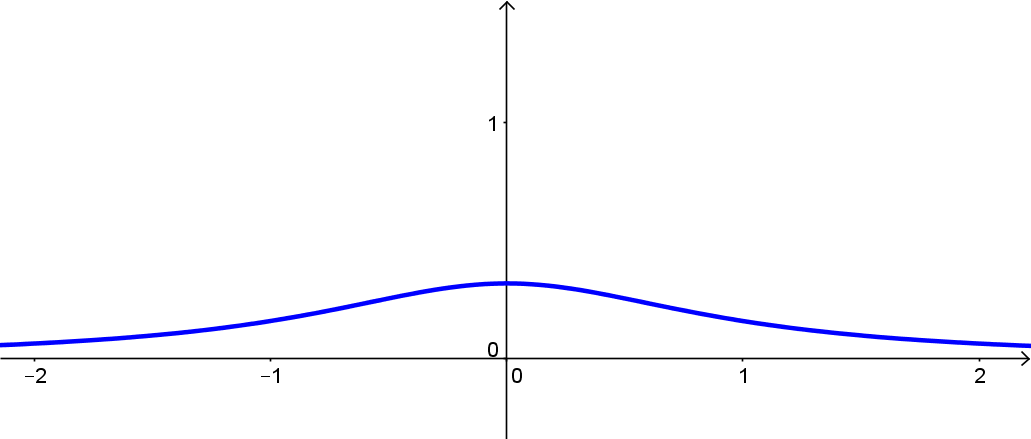
\includegraphics[width=12cm]{../fig/Cap05-DistribucionCauchy.png}\\
\end{enColor}
\begin{bn}
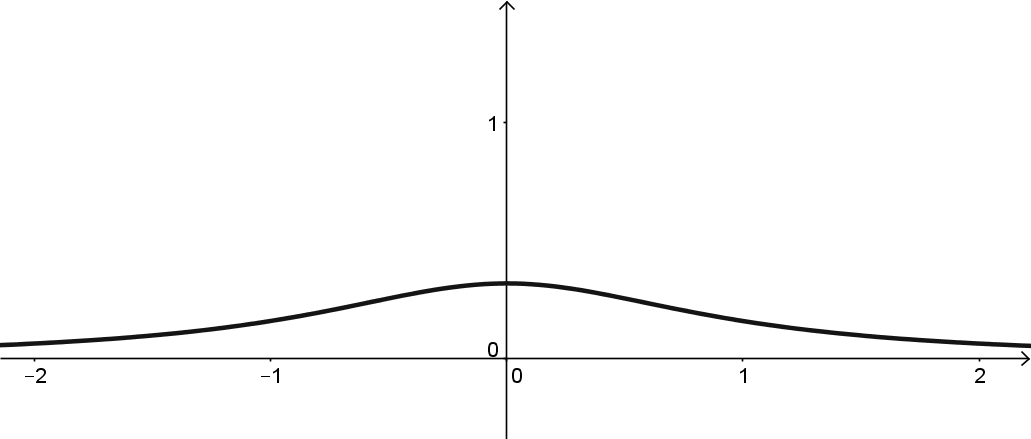
\includegraphics[width=12cm]{../fig/Cap05-DistribucionCauchy-bn.png}
\end{bn}
\caption{Un ejemplo de función de densidad para una variable aleatoria continua.}
\label{cap05:fig:DistribucionCauchy}
\end{center}
\end{figure}

    Hemos querido empezar con esta función porque es un ejemplo suficientemente sencillo, en el que el lector podrá ver el tipo de recursos que vamos a necesitar, pero a la vez no es engañosamente simple. En el Tutorial05 veremos cómo comprobar que esta función de densidad satisface la propiedad (b), que debe satisfacer cualquier función de densidad para ser digna de ese nombre. Aquí queremos centrarnos en aprender a utilizar esta función para calcular la probabilidad de un cierto intervalo. Por ejemplo, vamos a calcular
    \[P(0\leq X\leq 1)\]
    para esta variable aleatoria continua. Sabemos, por la Ecuación \ref{cap05:ecu:AsignacionProbabilidadIntegralDensidad}, que la forma de asignar la probabilidad a un intervalo es mediante la integral:
    \[P(a\leq X\leq b)=\int_a^b f(x)dx.\]
    En este ejemplo $(a,b)=(0,1)$, y $f(x)=\frac{1}{\pi(1+x^2)}$. Así que eso significa que debemos calcular esta integral:
    \[
    P(0\leq X\leq 1)=\int_0^1f(x)dx=\int_0^1\dfrac{1}{\pi(1+x^2)}dx,
    \]
    o, lo que es lo mismo, que tenemos que calcular el área sombreada de la Figura \ref{cap05:fig:DistribucionCauchy-2}. Vamos a introducir más terminología, y a dar algunos detalles técnicos, antes de retomar el ejemplo.
    \qed

\begin{figure}[htbp]
\begin{center}
\begin{enColor}
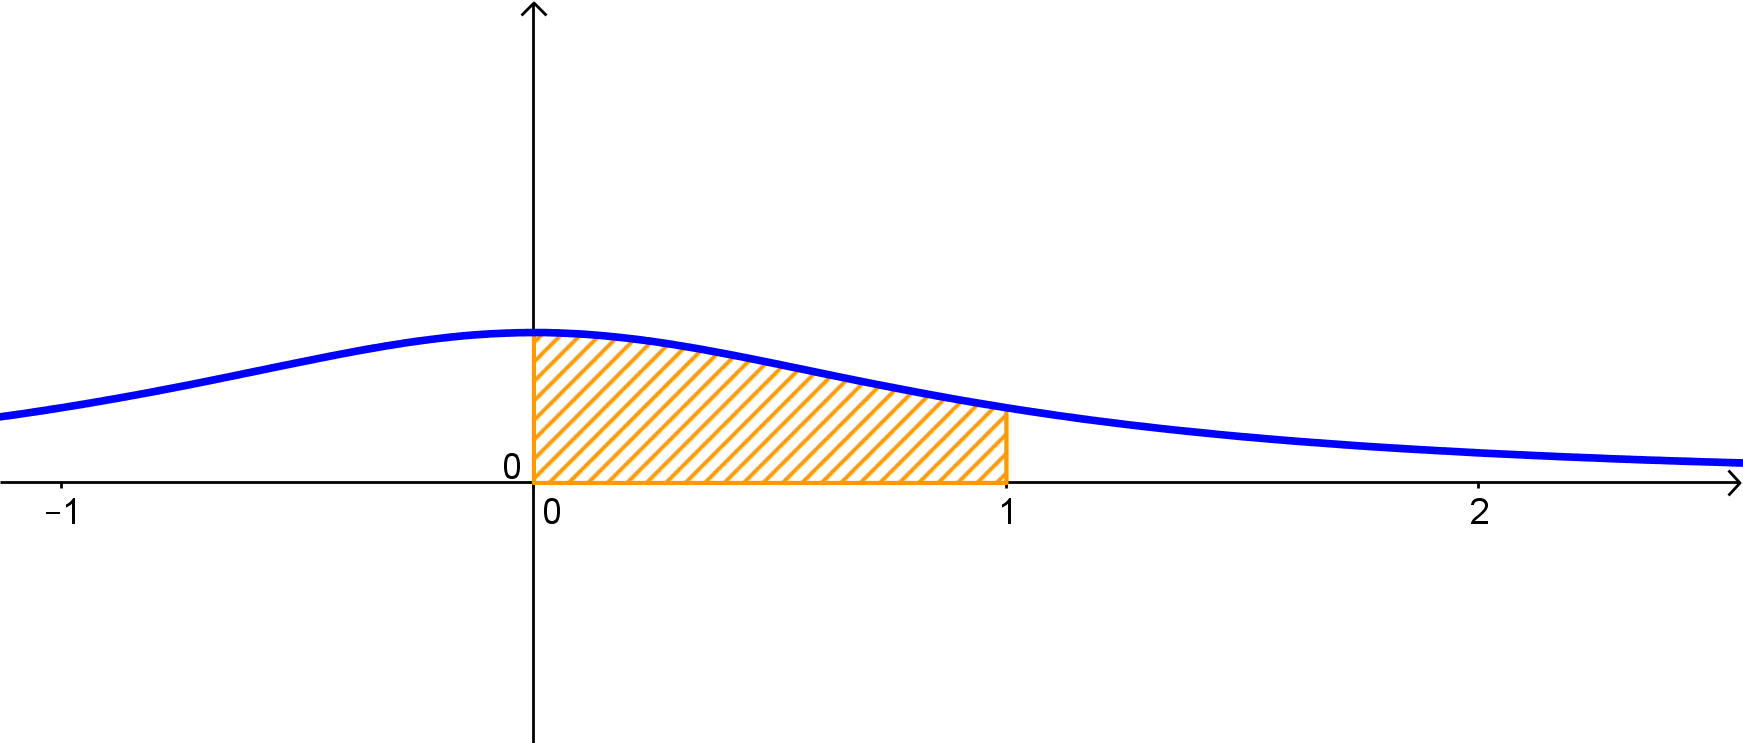
\includegraphics[width=12cm]{../fig/Cap05-DistribucionCauchy-2.png}
\end{enColor}
\begin{bn}
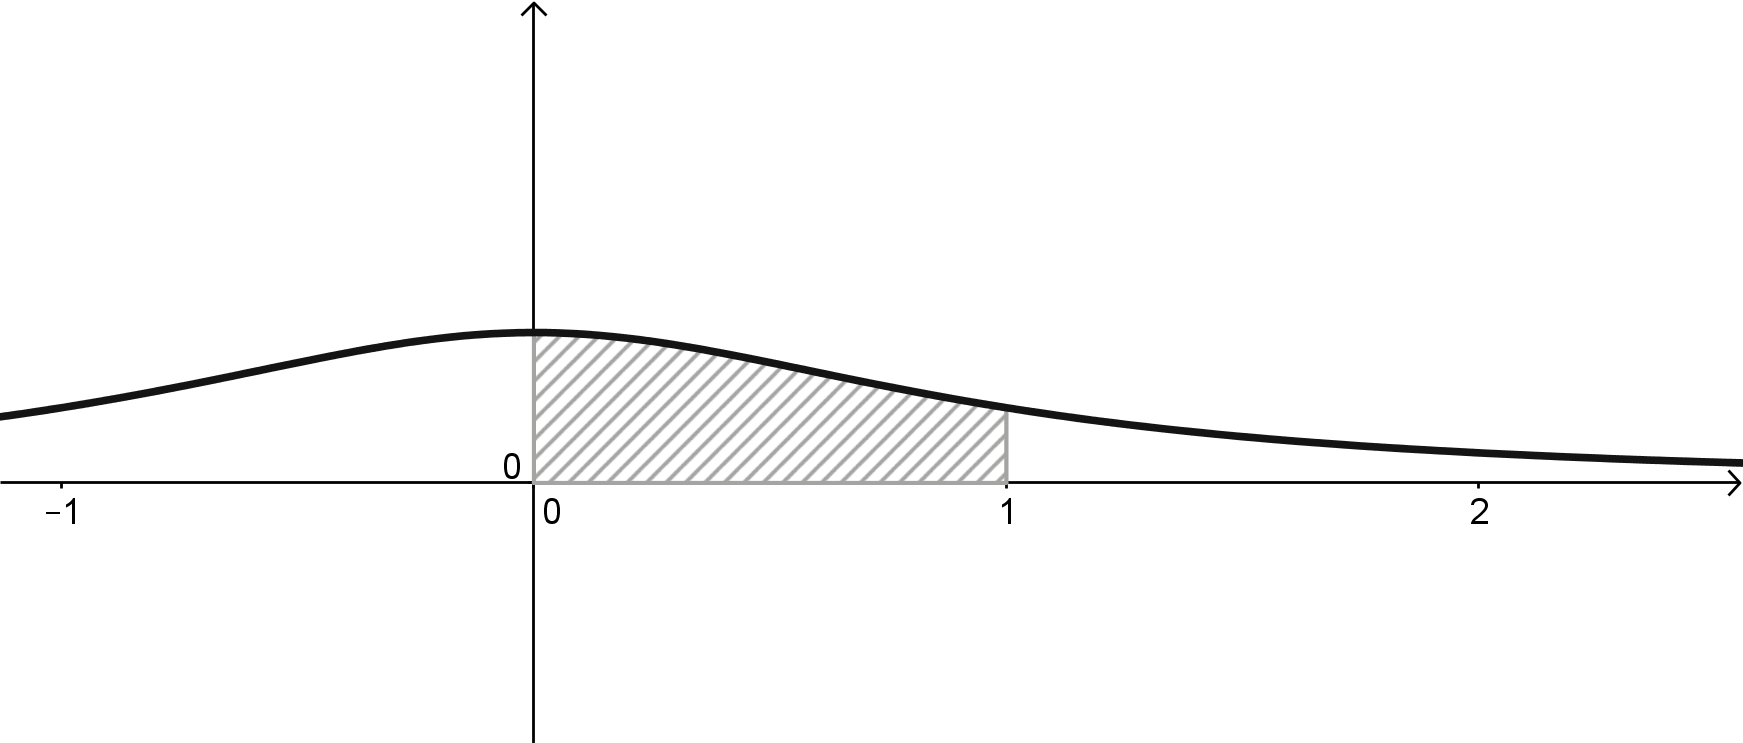
\includegraphics[width=12cm]{../fig/Cap05-DistribucionCauchy-2-bn.png}
\end{bn}
\caption{La probabilidad $P(0\leq X\leq 1)$ se calcula integrando $f(x)$ entre $0$ y $1$.}
\label{cap05:fig:DistribucionCauchy-2}
\end{center}
\end{figure}

\end{ejemplo}
¿Cómo se calcula la integral que ha aparecido en este ejemplo? En la inmensa mayoría de los casos, cuando se desea un resultado exacto (simbólico), el cálculo es un proceso en dos pasos, usando el método que se conoce como {\sf Teorema Fundamental del Cálculo Integral}\index{teorema fundamental del cálculo integral} (o Regla de Barrow)\index{regla de Barrow}:
    \begin{center}
    \fcolorbox{black}{Gris025}{
    \begin{minipage}{12cm}
        \begin{center}
        %%%%%%%%%%%%%%%%%%%%%%%%%%%%%%%%%%%%%%%
        {\bf Teorema Fundamental del Cálculo Integral}
        \index{teorema fundamental del cálculo integral}
        \end{center}
        %%%%%%%%%%%%%%%%%%%%%%%%%%%%%%%%%%%%%%%
        \begin{enumerate}
          \item Buscamos una función $F(x)$ que cumpla $F'(x)=f(x)$. Esa función $F$ se denomina una {\sf primitiva}\index{primitiva} de $f(x)$, también se representa mediante el símbolo de integral, pero sin que aparezcan los extremos del intervalo:
              \[F(x)=\int f(x)dx.\]
              La notación habitual para una primitiva es, como hemos hecho aquí, utilizar la misma letra pero en mayúsculas.
          \item Una vez que hemos hallado $F$, la integral (es decir, el área, es decir, la probabilidad) es igual a la diferencia de valores de $F$ en los extremos del intervalo:
              \begin{equation}\label{cap05:ecu:TeoremaFundamentalCalculo}
              \int_a^b f(x)dx = F(b)-F(a).
              \end{equation}
        \end{enumerate}
        %%%%%%%%%%%%%%%%%%%%%%%%%%%%%%%%%%%%%%%
    \end{minipage}}
    \end{center}
Como puede verse, este método descansa sobre nuestra capacidad de calcular una primitiva de $F$. Esa operación puede ser muy difícil, o incluso imposible en algunos casos (volveremos sobre esto). Y tradicionalmente, los estudios de Matemáticas consagraban mucho tiempo y esfuerzo a aprender los métodos para encontrar primitivas. Afortunadamente, en la segunda mitad del siglo XX esa tarea se ha mecanizado, y ahora podemos dejar que los ordenadores se encarguen del trabajo más tedioso. Existen muchos programas, accesibles incluso mediante páginas web, desde un teléfono móvil, que calculan primitivas en todos los casos que vamos a necesitar. En el Tutorial05 veremos varios de estos programas, y practicaremos su uso. Volvamos al ejemplo.
\begin{ejemplo}[Continuación del Ejemplo \ref{cap05:ejem:CalculoProbabilidadIntegralParte1}]
\label{cap05:ejem:CalculoProbabilidadIntegralParte2}
Usando alguno de los recursos que conoceremos en el Tutorial05, obtenemos una primitiva de $f(x)=\frac{1}{\pi(1+x^2)}$. El resultado es:
\[F(x)=\int f(x)dx=\int \frac{1}{\pi(1+x^2)} dx = \dfrac{1}{\pi}\arctan x.\]
Eso significa que si calculas la derivada de
\[F(x)=\dfrac{1}{\pi}\arctan x,\]
el resultado tiene que ser $f(x)$, la función de densidad (si sabes suficiente de derivación, que es mucho más fácil que la integración, siempre puedes (debes) comprobar a mano este tipo de afirmaciones).

Ahora podemos usar esta primitiva para calcular la probabilidad:
    \[
    P(0\leq X\leq 1)=\int_0^1f(x)dx=F(1)-F(0)=\]
    \[\left(\dfrac{1}{\pi}\arctan 1\right)-\left(\dfrac{1}{\pi}\arctan 0\right)=\dfrac{1}{4}-0=\dfrac{1}{4}
    \]
Así que la probabilidad que buscábamos es $\dfrac{1}{4}$.
\qed
\end{ejemplo}
En este ejemplo hemos puesto el énfasis en el cálculo de primitivas para que el lector pueda entender el método con algo más de detalle. Pero los mismos programas que calculan primitivas permiten calcular la integral
\[\int_0^1\dfrac{1}{\pi(1+x^2)}dx\]
en un sólo paso. De nuevo, nos remitimos al Tutorial05, donde veremos con más detalle las dos formas de proceder. Dejamos al lector la tarea de usar uno de estos programas para comprobar que la función de densidad del ejemplo cumple la propiedad (b) de las funciones de densidad (ver la página \pageref{cap05:ecu:AsignacionProbabilidadIntegralDensidad}). Esa propiedad garantiza que la probabilidad total es 1, y eso, como sabemos, es una de las Propiedades Fundamentales de la Probabilidad (pág. \pageref{cap03:def:PropiedadesFundamentalesFuncionProbabilidad}). Nosotros vamos a hacer esa comprobación usando la primitiva que hemos hallado, para así tener la ocasión de discutir algunos aspectos adicionales.

Antes de eso, un consejo, a modo de advertencia, dirigido a aquellos lectores con menos entrenamiento matemático. Sabemos que algunos de estos ejemplos, usando integrales y otros recursos técnicos, pueden resultar difíciles de digerir al principio. El consejo es que no hay que quedarse atascado en ellos. Las integrales nos sirven, simplemente, para hacer cálculos relacionados con probabilidades en variables continuas. Si ahora no entiendes algún ejemplo, trata sólo de captar la idea general, que suele estar más o menos clara, y sigue adelante. Con la práctica, después de ver varios casos, y hacer algunos ejercicios, las cosas irán quedando más claras, y podrás volver a leer el ejemplo que se te atragantó. Seguramente, lo entenderás mejor. Pero si, finalmente, no es así, asegúrate de pedir ayuda a alguien que sepa más de Matemáticas.
\begin{ejemplo}
\label{cap05:ejem:DistribucionCauchyIntegralTotal1}
    Vamos a utilizar la primitiva que hemos hallado en el Ejemplo \ref{cap05:ejem:CalculoProbabilidadIntegralParte2}, para comprobar que se cumple
    \[\int_{-\infty}^{\infty}\dfrac{1}{\pi(1+x^2)}dx=1.\]
    Nos vamos a detener en esto, porque queremos que el lector compruebe que, en muchos casos, la presencia del símbolo $\infty$ no supone ninguna complicación excesiva. Procedemos como en el Ejemplo \ref{cap05:ejem:CalculoProbabilidadIntegralParte2}. Tenemos la primitiva:
    \[F(x)=\int f(x)dx=\int \frac{1}{\pi(1+x^2)} dx = \dfrac{1}{\pi}\arctan x.\]
    Y usando el Teorema Fundamental del Cálculo obtenemos:
    \[\int_{-\infty}^{\infty}\dfrac{1}{\pi(1+x^2)}dx=F(\infty)-F(-\infty).\]
    ¿Qué significa $F(\infty)$? Sustituyendo ingenuamente, como si infinito fuera un número cualquiera, obtenemos
    \[\dfrac{1}{\pi}\arctan(\infty).\]
    Así que la pregunta pasa a ser ``¿qué significa $\arctan(\infty)$?''. La respuesta técnica es que tendríamos que calcular un límite. Pero en este, y en muchos otros casos, podemos tomar un camino más sencillo. Cuando un matemático ve un símbolo como $\infty$, sabe que casi siempre eso significa que debemos preguntarnos lo que sucede cuando pensamos en valores muy grandes de la variable; de hecho, tan grandes como se quiera. Vamos a representar la gráfica de la función $F(x)$, que puede verse en la Figura \ref{cap05:fig:Cap05-GraficaArcoTangente}.

\begin{figure}[htbp]
\begin{center}
\begin{enColor}
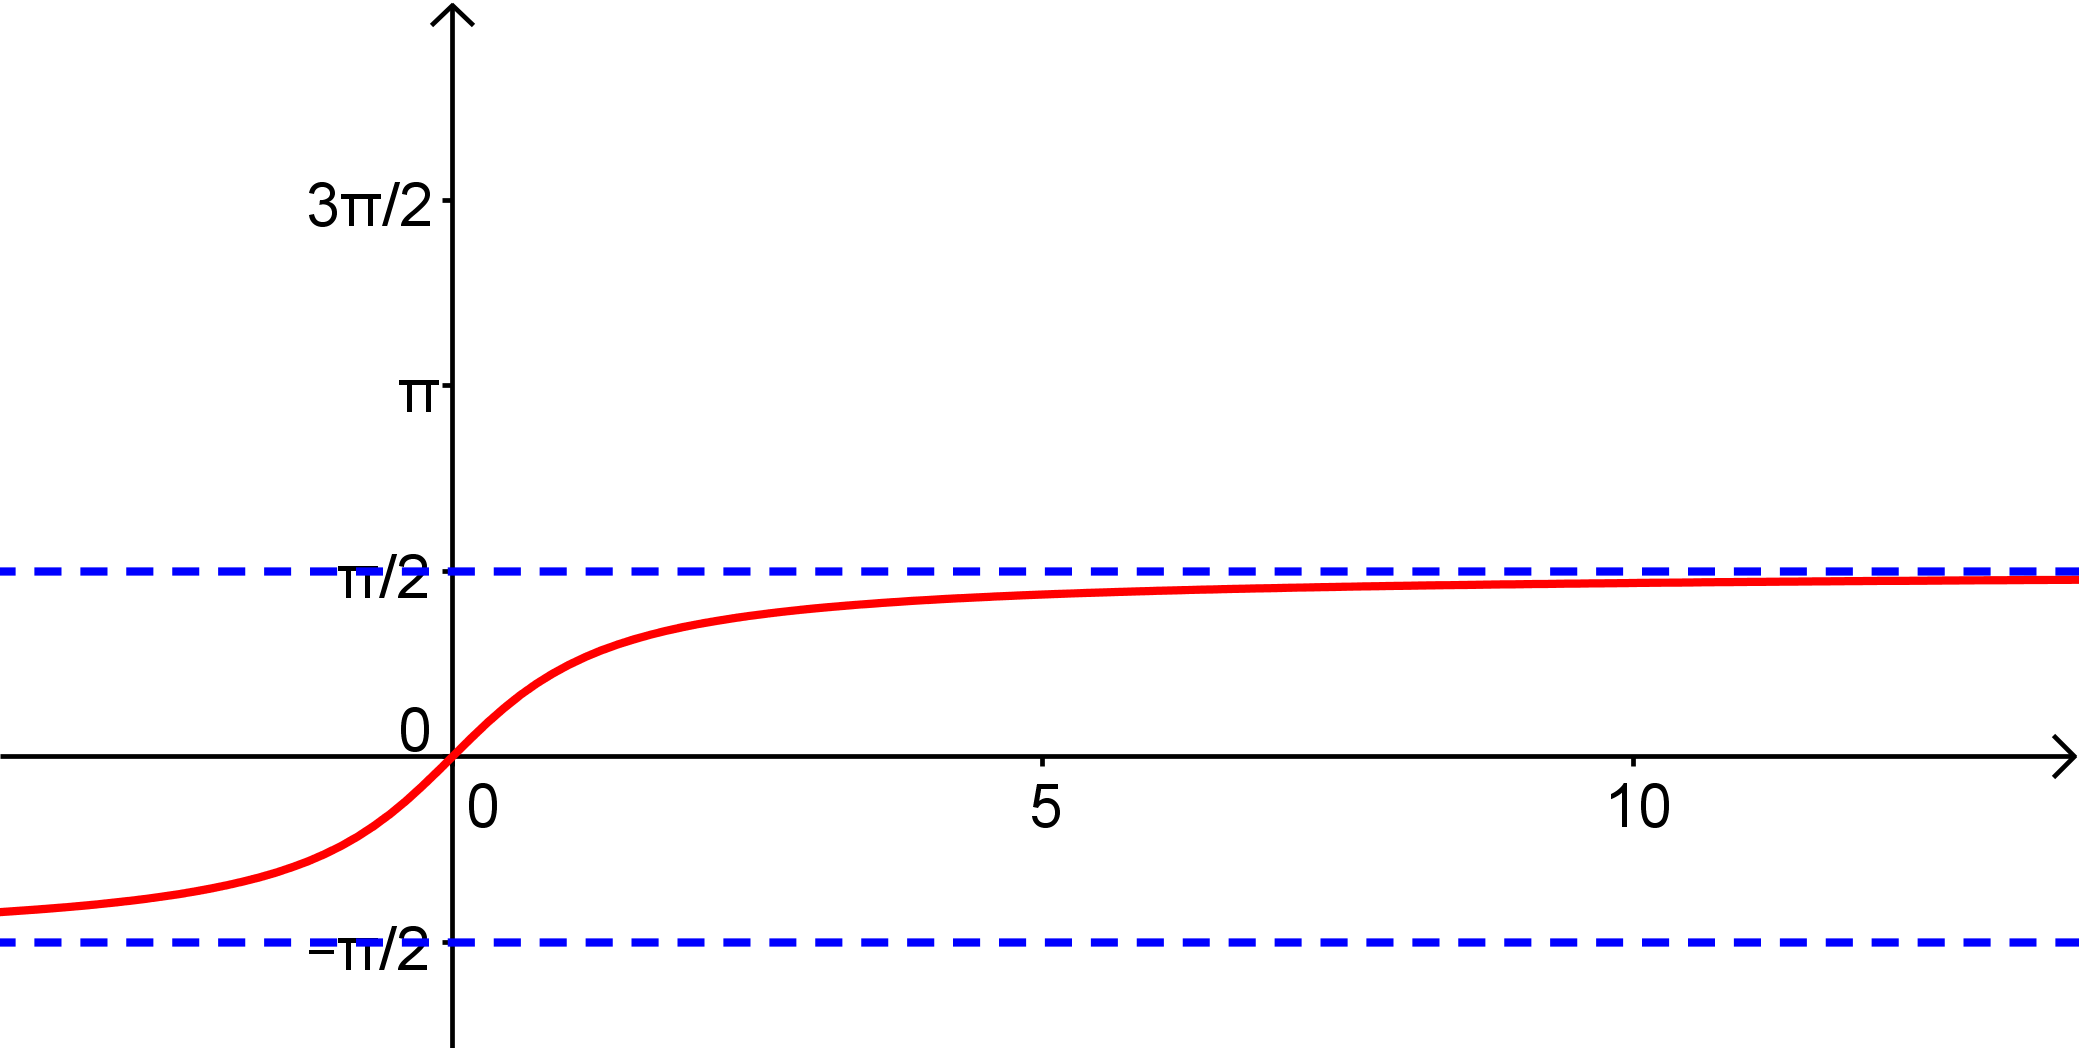
\includegraphics[width=12cm]{../fig/Cap05-GraficaArcoTangente.png}
\end{enColor}
\begin{bn}
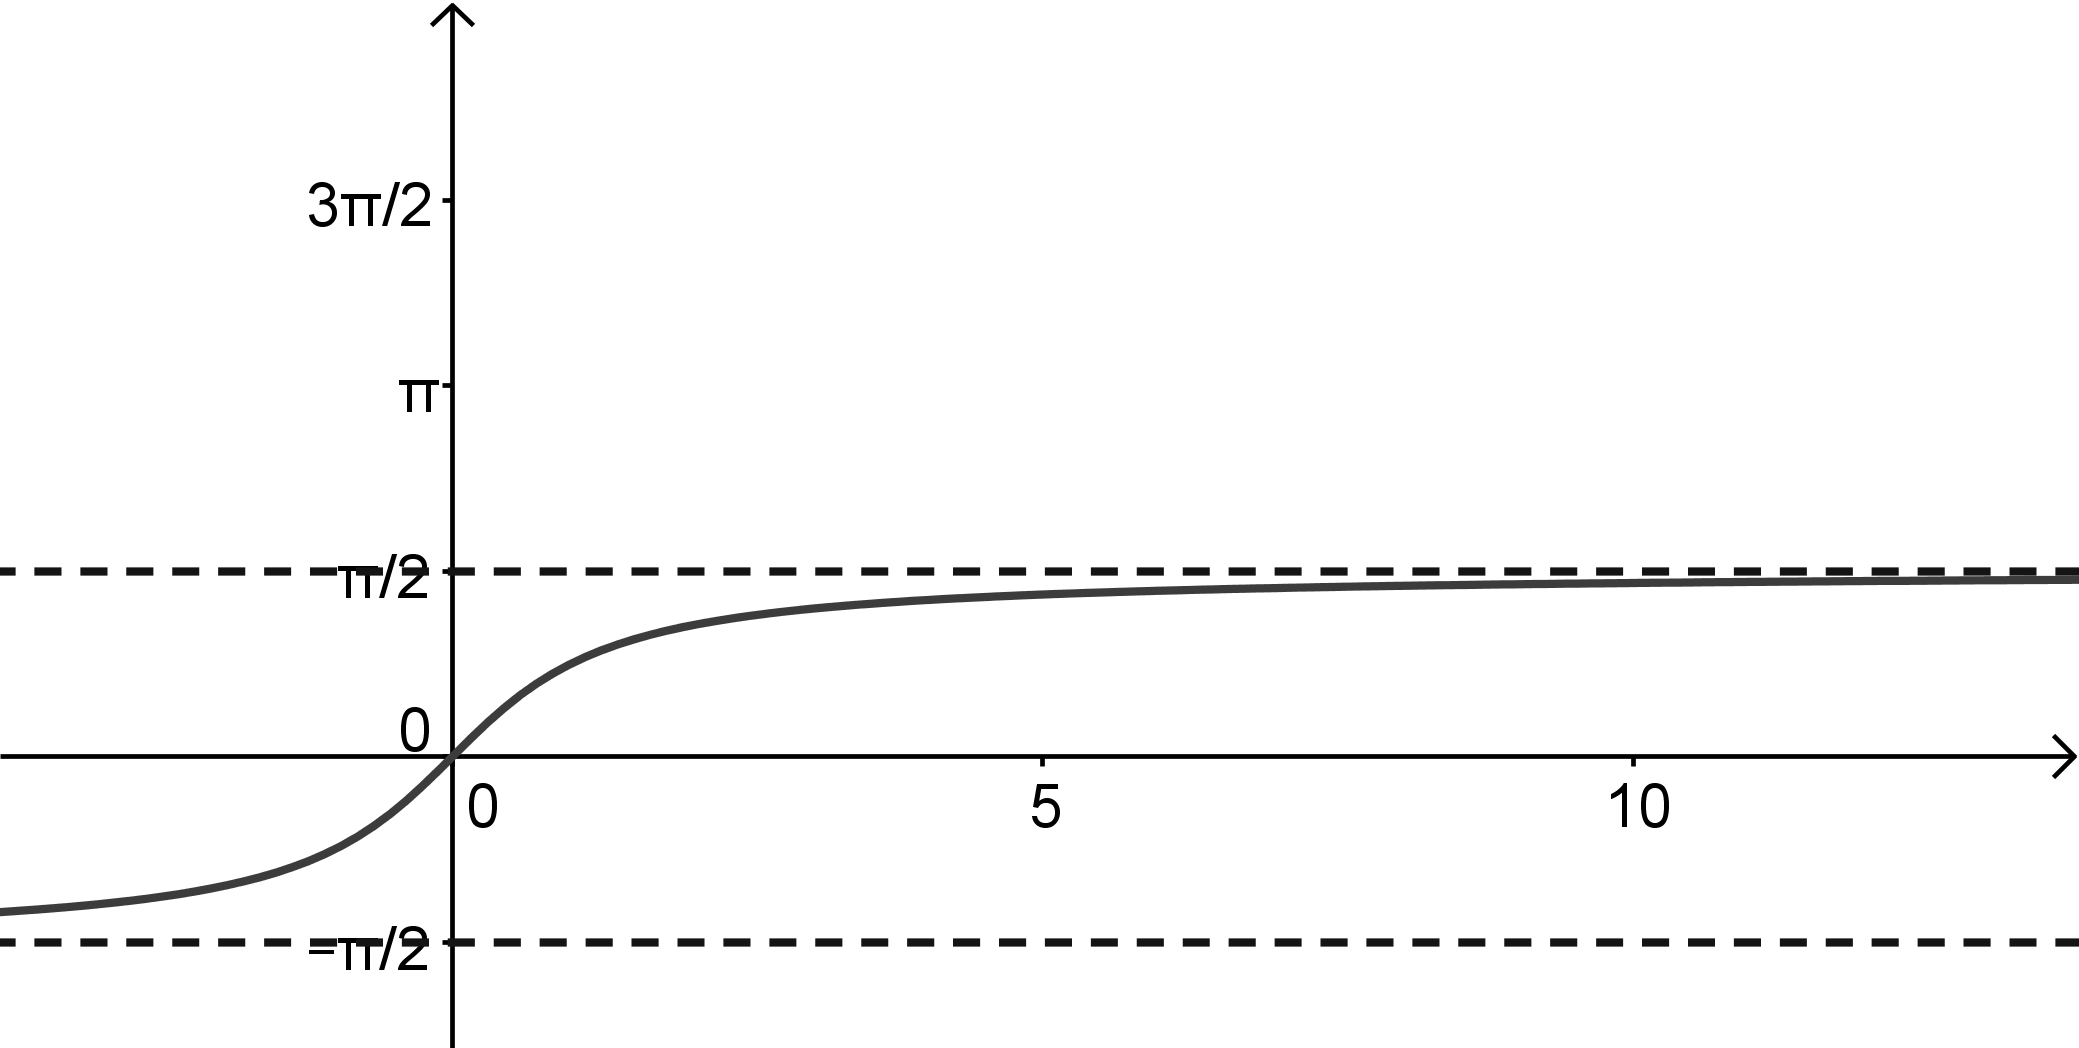
\includegraphics[width=12cm]{../fig/Cap05-GraficaArcoTangente-bn.png}
\end{bn}
\caption{Gráfica de la función $F(x)$ del Ejemplo \ref{cap05:ejem:DistribucionCauchyIntegralTotal1}.}
\label{cap05:fig:Cap05-GraficaArcoTangente}
\end{center}
\end{figure}

    Hemos añadido dos líneas de trazos a esa figura para hacer ver que, para valores muy grandes de $x$, de hecho, cuanto más grande sea $x$, más se parece el valor de $\arctan(x)$ a $\dfrac{\pi}{2}$. Así que podemos decir, sin temor a equivocarnos, que
    \[\arctan(\infty)=\dfrac{\pi}{2}.\]
    Y de la misma forma:
    \[\arctan(-\infty)=-\dfrac{\pi}{2}.\]
    Por lo tanto, la integral (de probabilidad total) que tratábamos de calcular es (atención al $1/\pi$ en $F$):
    \[\int_{-\infty}^{\infty}\dfrac{1}{\pi(1+x^2)}dx=F(\infty)-F(-\infty)=\]
    \[\dfrac{1}{\pi}\arctan(\infty)-\dfrac{1}{\pi}\arctan(-\infty)=
    \dfrac{1}{\pi}\left(\dfrac{\pi}{2}\right)-\dfrac{1}{\pi}\left(-\dfrac{\pi}{2}\right)=1.\]
    \qed
\end{ejemplo}
Esta propiedad de las funciones de densidad, el hecho de que la integral total vale 1, nos será de mucha utilidad para ahorrarnos algunos cálculos. El siguiente ejemplo pretende ilustrar esto:
\begin{ejemplo}\label{cap05:ejem:DistribucionCauchyTrucosProbabilidad}
    Todavía con la función del Ejemplo \ref{cap05:ejem:CalculoProbabilidadIntegralParte1}, vamos a calcular la probabilidad:
    \[
    P(X>1)=\int_1^{\infty}f(x)dx
    \]
    Es decir, el área sombreada de la Figura \ref{cap05:fig:Cap05-DistribucionCauchy-IntegralColaDerecha}. Se trata de un intervalo {\em no acotado}, que se extiende hasta infinito.

\begin{figure}[htbp]
\begin{center}
\begin{enColor}
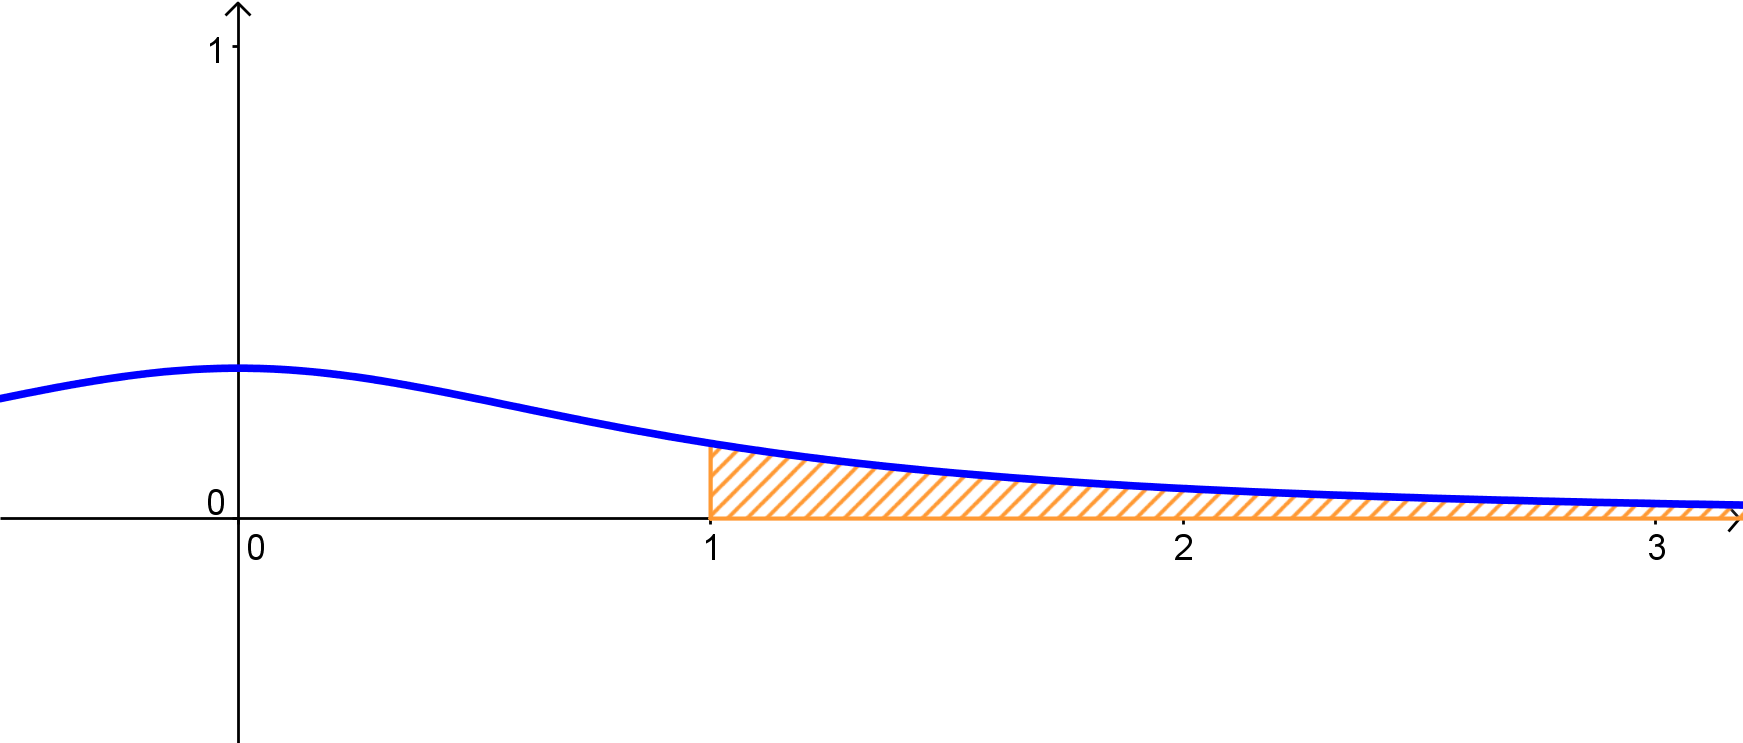
\includegraphics[width=12cm]{../fig/Cap05-DistribucionCauchy-IntegralColaDerecha.png}
\end{enColor}
\begin{bn}
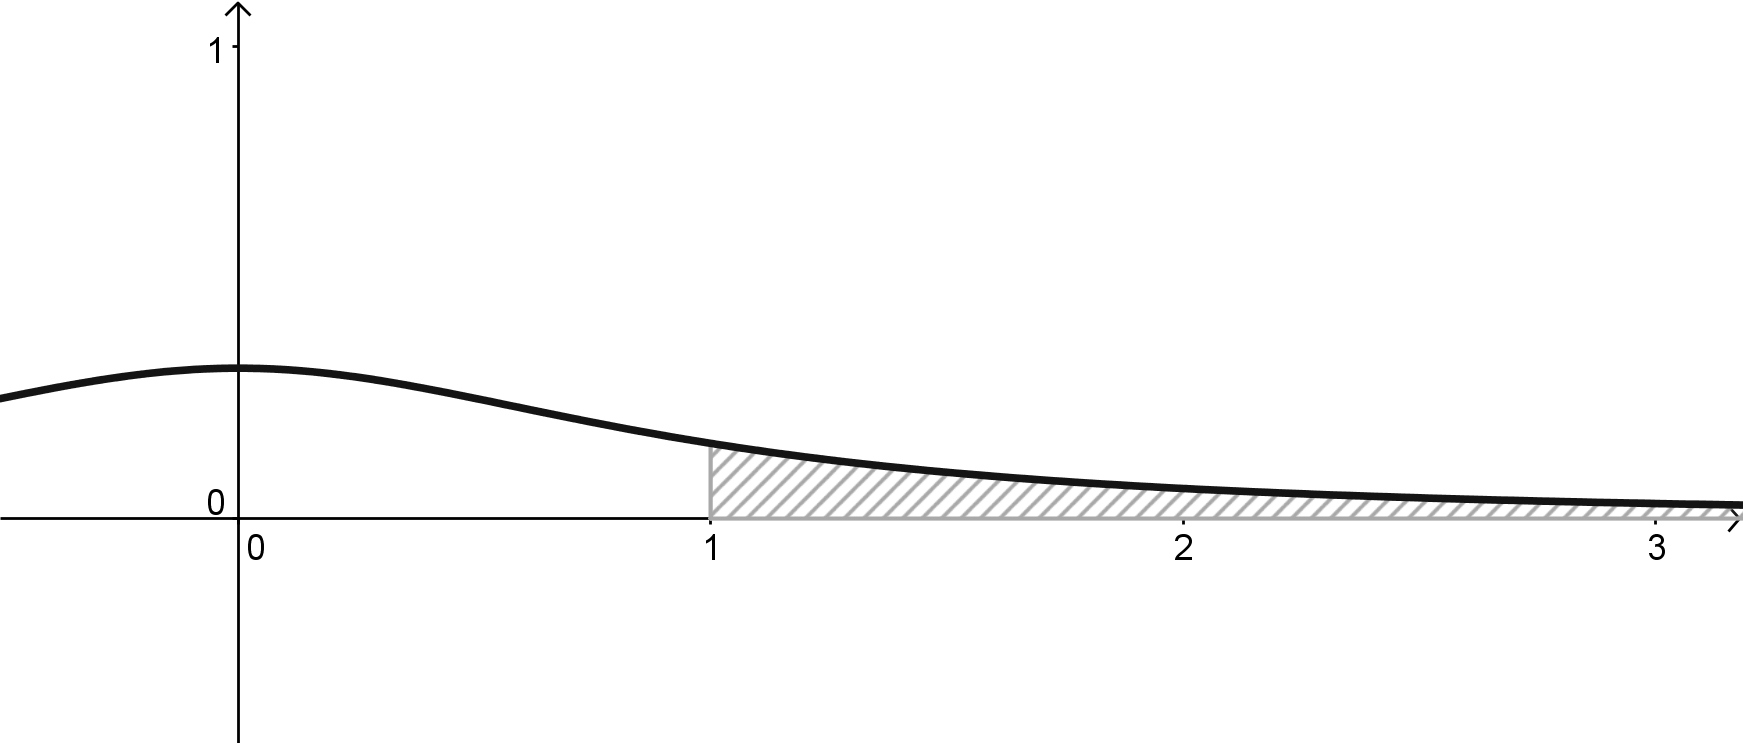
\includegraphics[width=12cm]{../fig/Cap05-DistribucionCauchy-IntegralColaDerecha-bn.png}
\end{bn}
\caption{Cálculo de probabilidad para un intervalo no acotado.}
\label{cap05:fig:Cap05-DistribucionCauchy-IntegralColaDerecha}
\end{center}
\end{figure}

    Usando la primitiva del Ejemplo \ref{cap05:ejem:CalculoProbabilidadIntegralParte2}, obtenemos:
    \[
    P(X>1)=\int_1^{\infty}f(x)dx=\dfrac{1}{\pi}\arctan(\infty)-\dfrac{1}{\pi}\arctan(1)=
    \dfrac{1}{\pi}\cdot\dfrac{\pi}{2}-\dfrac{1}{\pi}\cdot\dfrac{\pi}{4}=\dfrac{1}{4}.
    \]
    No hay ninguna dificultad en esto. Pero queremos usar este ejemplo para ilustrar otra forma de trabajar que a menudo será útil, aprovechándonos de la simetría de la función $f(x)$. El método se ilustra en los comentarios de la Figura \ref{cap05:fig:Cap05-DistribucionCauchy-TrucosIntegral-rotulado-bn.png}, que debes leer en el orden que se indica.

\begin{figure}[htbp]
\begin{center}
\begin{enColor}
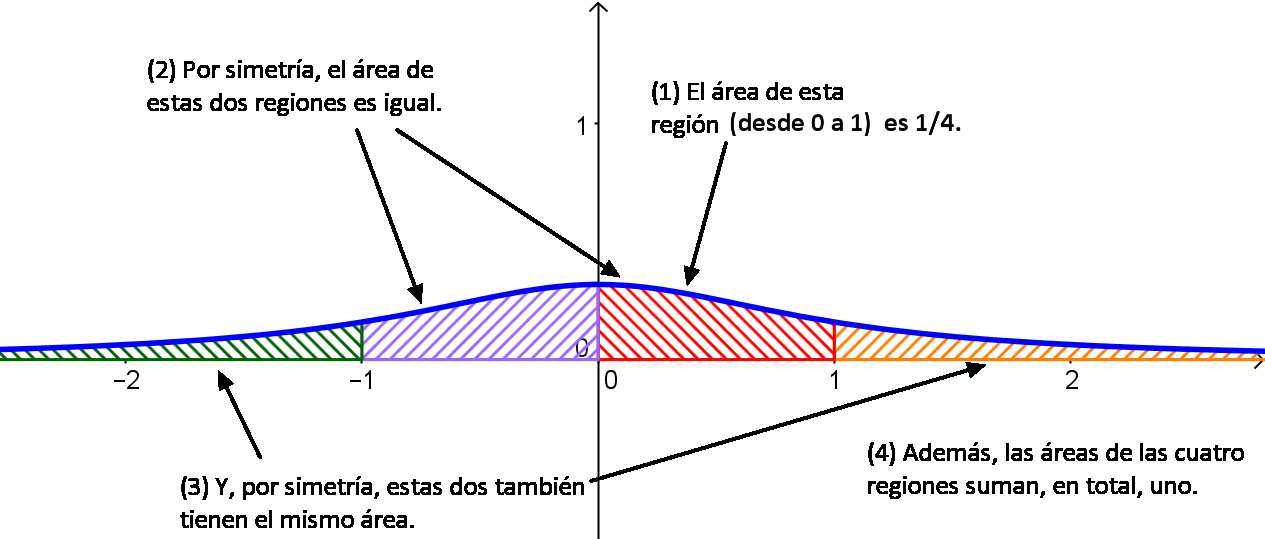
\includegraphics[width=12cm]{../fig/Cap05-DistribucionCauchy-TrucosIntegral-rotulado.png}
\end{enColor}
\begin{bn}
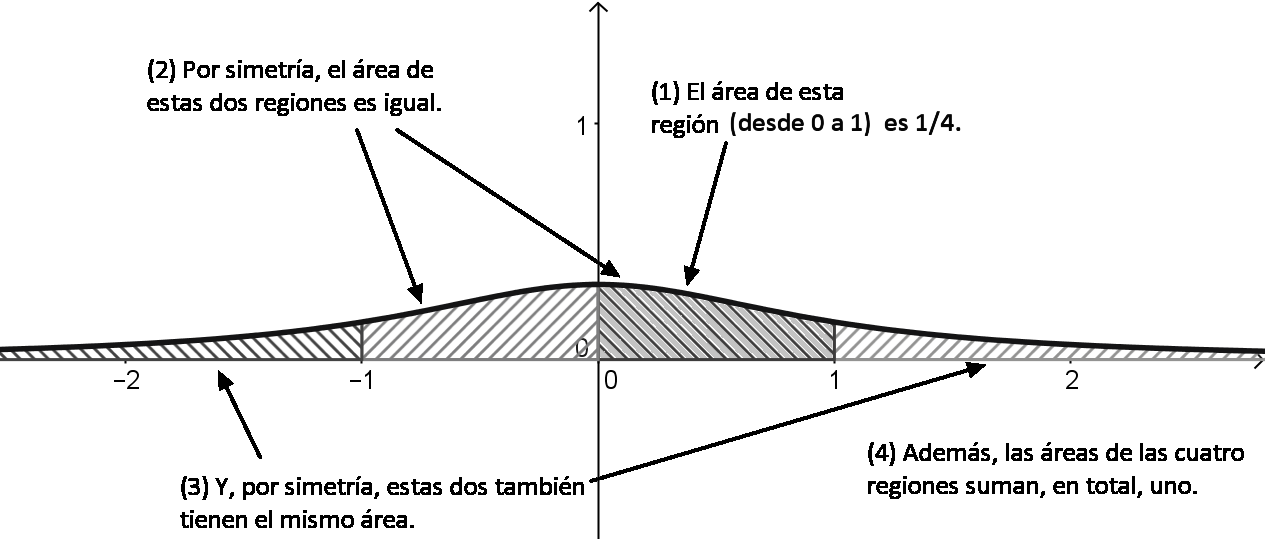
\includegraphics[width=12cm]{../fig/Cap05-DistribucionCauchy-TrucosIntegral-rotulado-bn.png}
\end{bn}
\caption{Cálculo de probabilidad mediante descomposición en intervalos simétricos.}
\label{cap05:fig:Cap05-DistribucionCauchy-TrucosIntegral-rotulado-bn.png}
\end{center}
\end{figure}

    Como puede verse, el método consiste en descomponer el área total, que es uno, en cuatro regiones, iguales dos a dos por simetría. Como sabemos (por el Ejemplo \ref{cap05:ejem:CalculoProbabilidadIntegralParte2}) que:
    \[P(0<X<1)=\dfrac{1}{4},\]
    deducimos, para el intervalo simétrico, que:
    \[P(-1<X<0)=\dfrac{1}{4}.\]
    Así que, uniendo ambos intervalos:
    \[P(-1<X<1)=\dfrac{1}{2}\]
    (¿Qué propiedades de la probabilidad de la unión hemos usado aquí?) Se deduce que la probabilidad del complementario también debe ser $1/2$. Es decir,
    \[P\bigl((X<-1)\cup(X>1)\bigr)=P(X<-1)+P(X>1)=\dfrac{1}{2}.\]
    (Insistimos: ¿qué propiedades de la probabilidad de la unión estamos usando?) Y como, otra vez por simetría, sabemos que:
    \[P(X<-1)=P(X>1),\]
    podemos despejar
    \[P(X>1)=\dfrac{1}{4},\]
    el mismo resultado que antes, pero evitando la integración. \qed
\end{ejemplo}
Con la práctica, este tipo de trucos basados en la simetría y la descomposición en intervalos de probabilidad conocida, se vuelven cada vez más naturales, hasta que conseguimos hacerlos simplemente mirando la figura correspondiente. Es muy bueno, y no nos cansaremos de insistir en esto, acostumbrarse a razonar sobre las figuras. Cuando empecemos a trabajar sobre Inferencia Estadística volveremos sobre esto, y trataremos de persuadir al lector de que un pequeño esbozo de una figura puede evitarle muchos quebraderos de cabeza, y más de un error.

Esperamos que estos ejemplos ayuden al lector a empezar a entender el papel que interpreta la función de densidad de una variable continua. En particular, vemos que si $X$ es una variable aleatoria continua y  $f(x)$ es su función de densidad, la función $f$ representa una forma de repartir la probabilidad total (que siempre es uno) entre los puntos de la recta real, de manera que las zonas donde $f(x)$ vale más son las zonas con mayor probabilidad. Esto se ilustra en la Figura \ref{cap05:fig:Cap05-InterpretacionFuncionDensidadFicticia-bn.png}, para una función de densidad ficticia:

\begin{figure}[htbp]
\begin{center}
\begin{enColor}
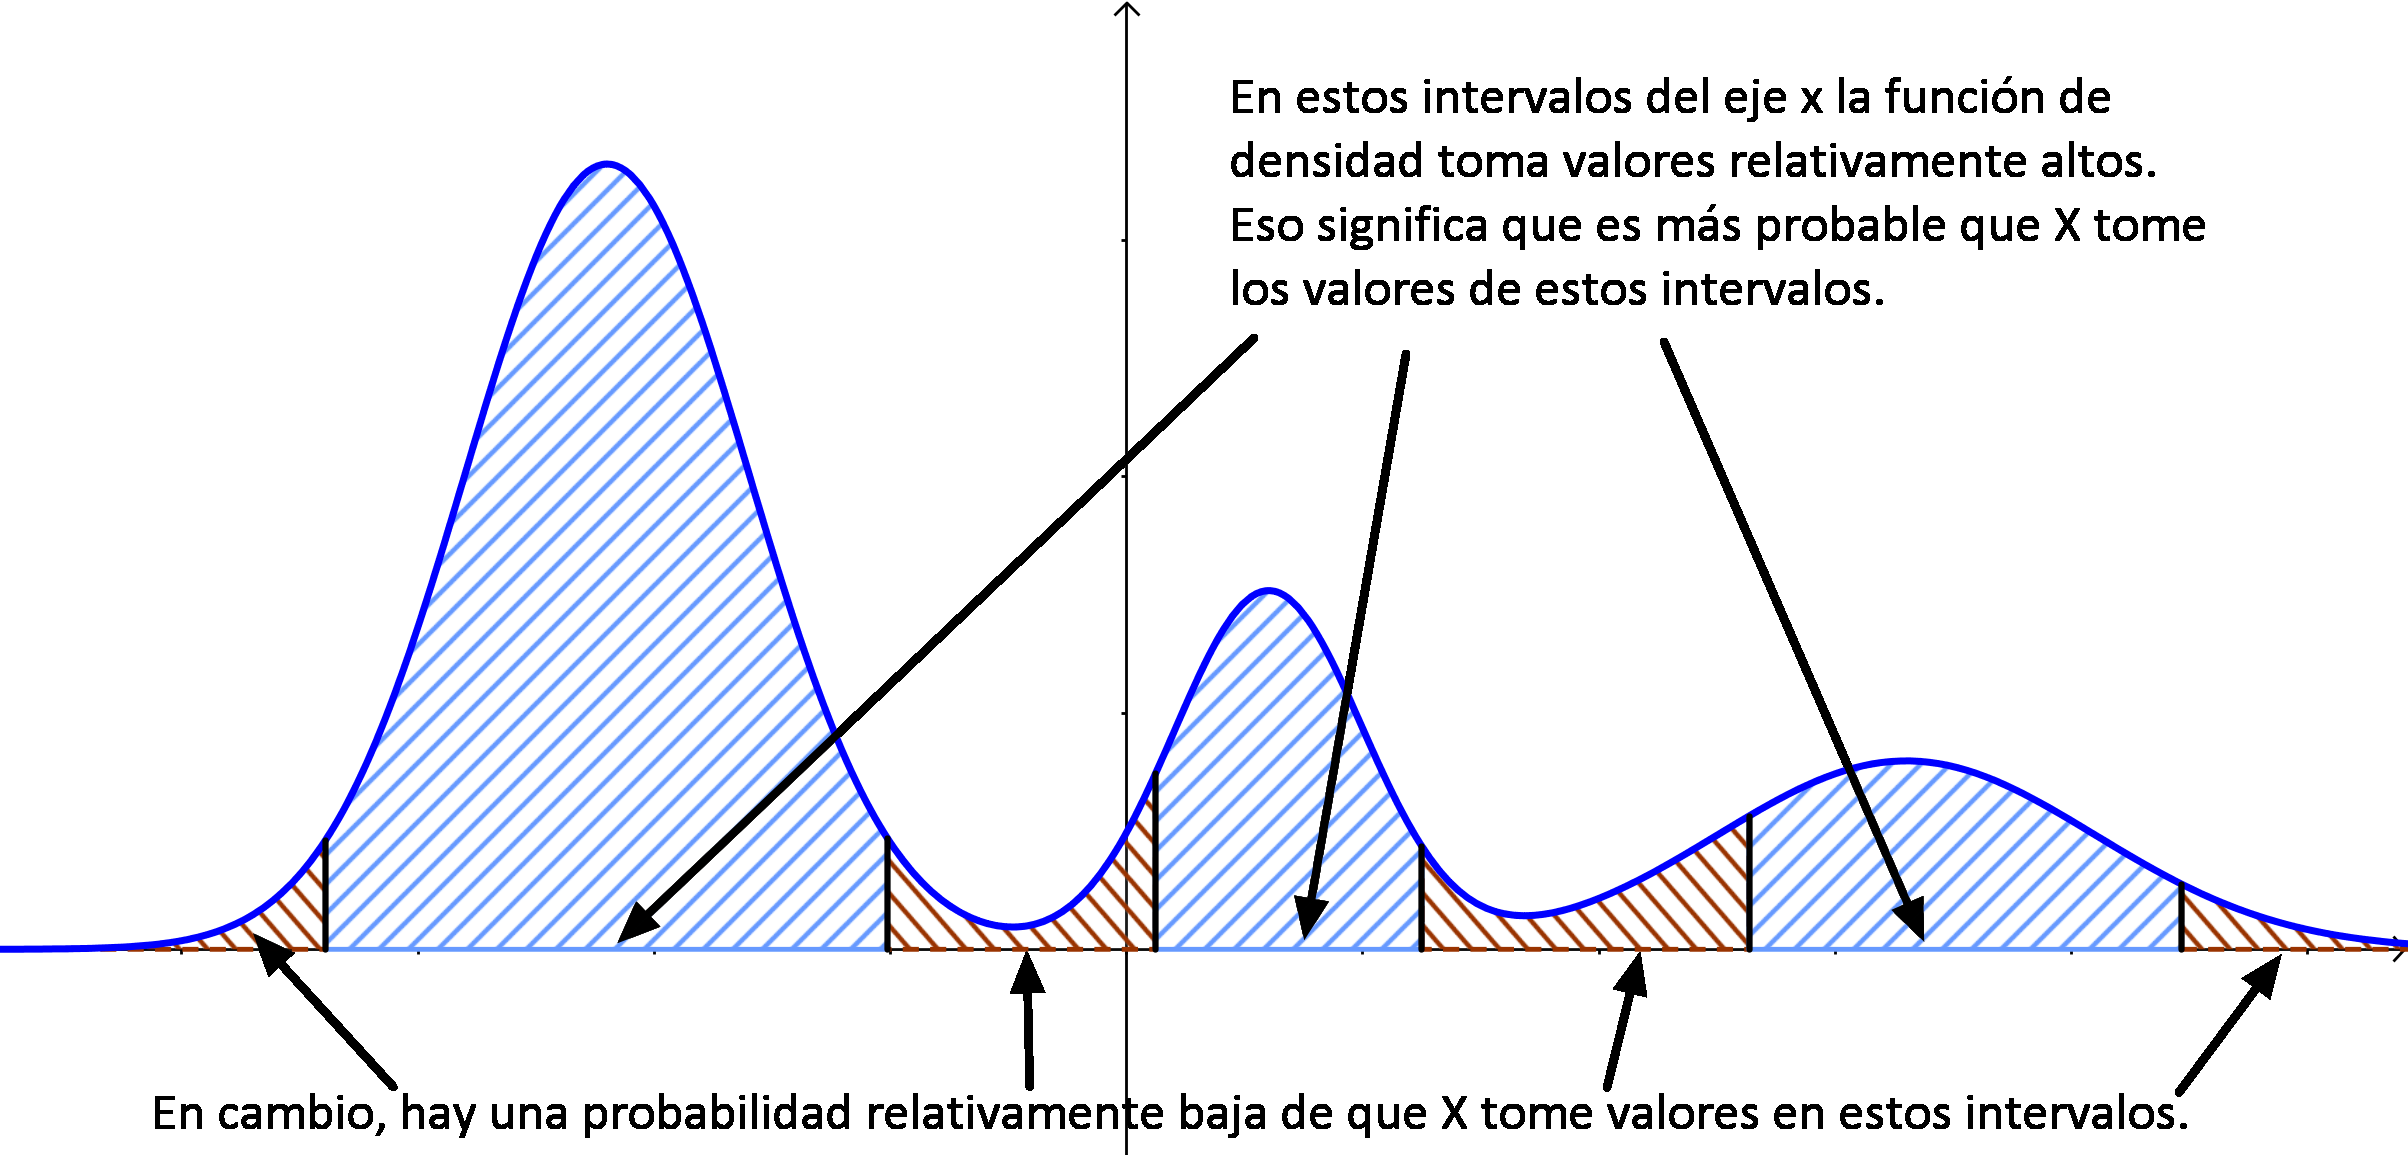
\includegraphics[width=12cm]{../fig/Cap05-InterpretacionFuncionDensidadFicticia.png}
\end{enColor}
\begin{bn}
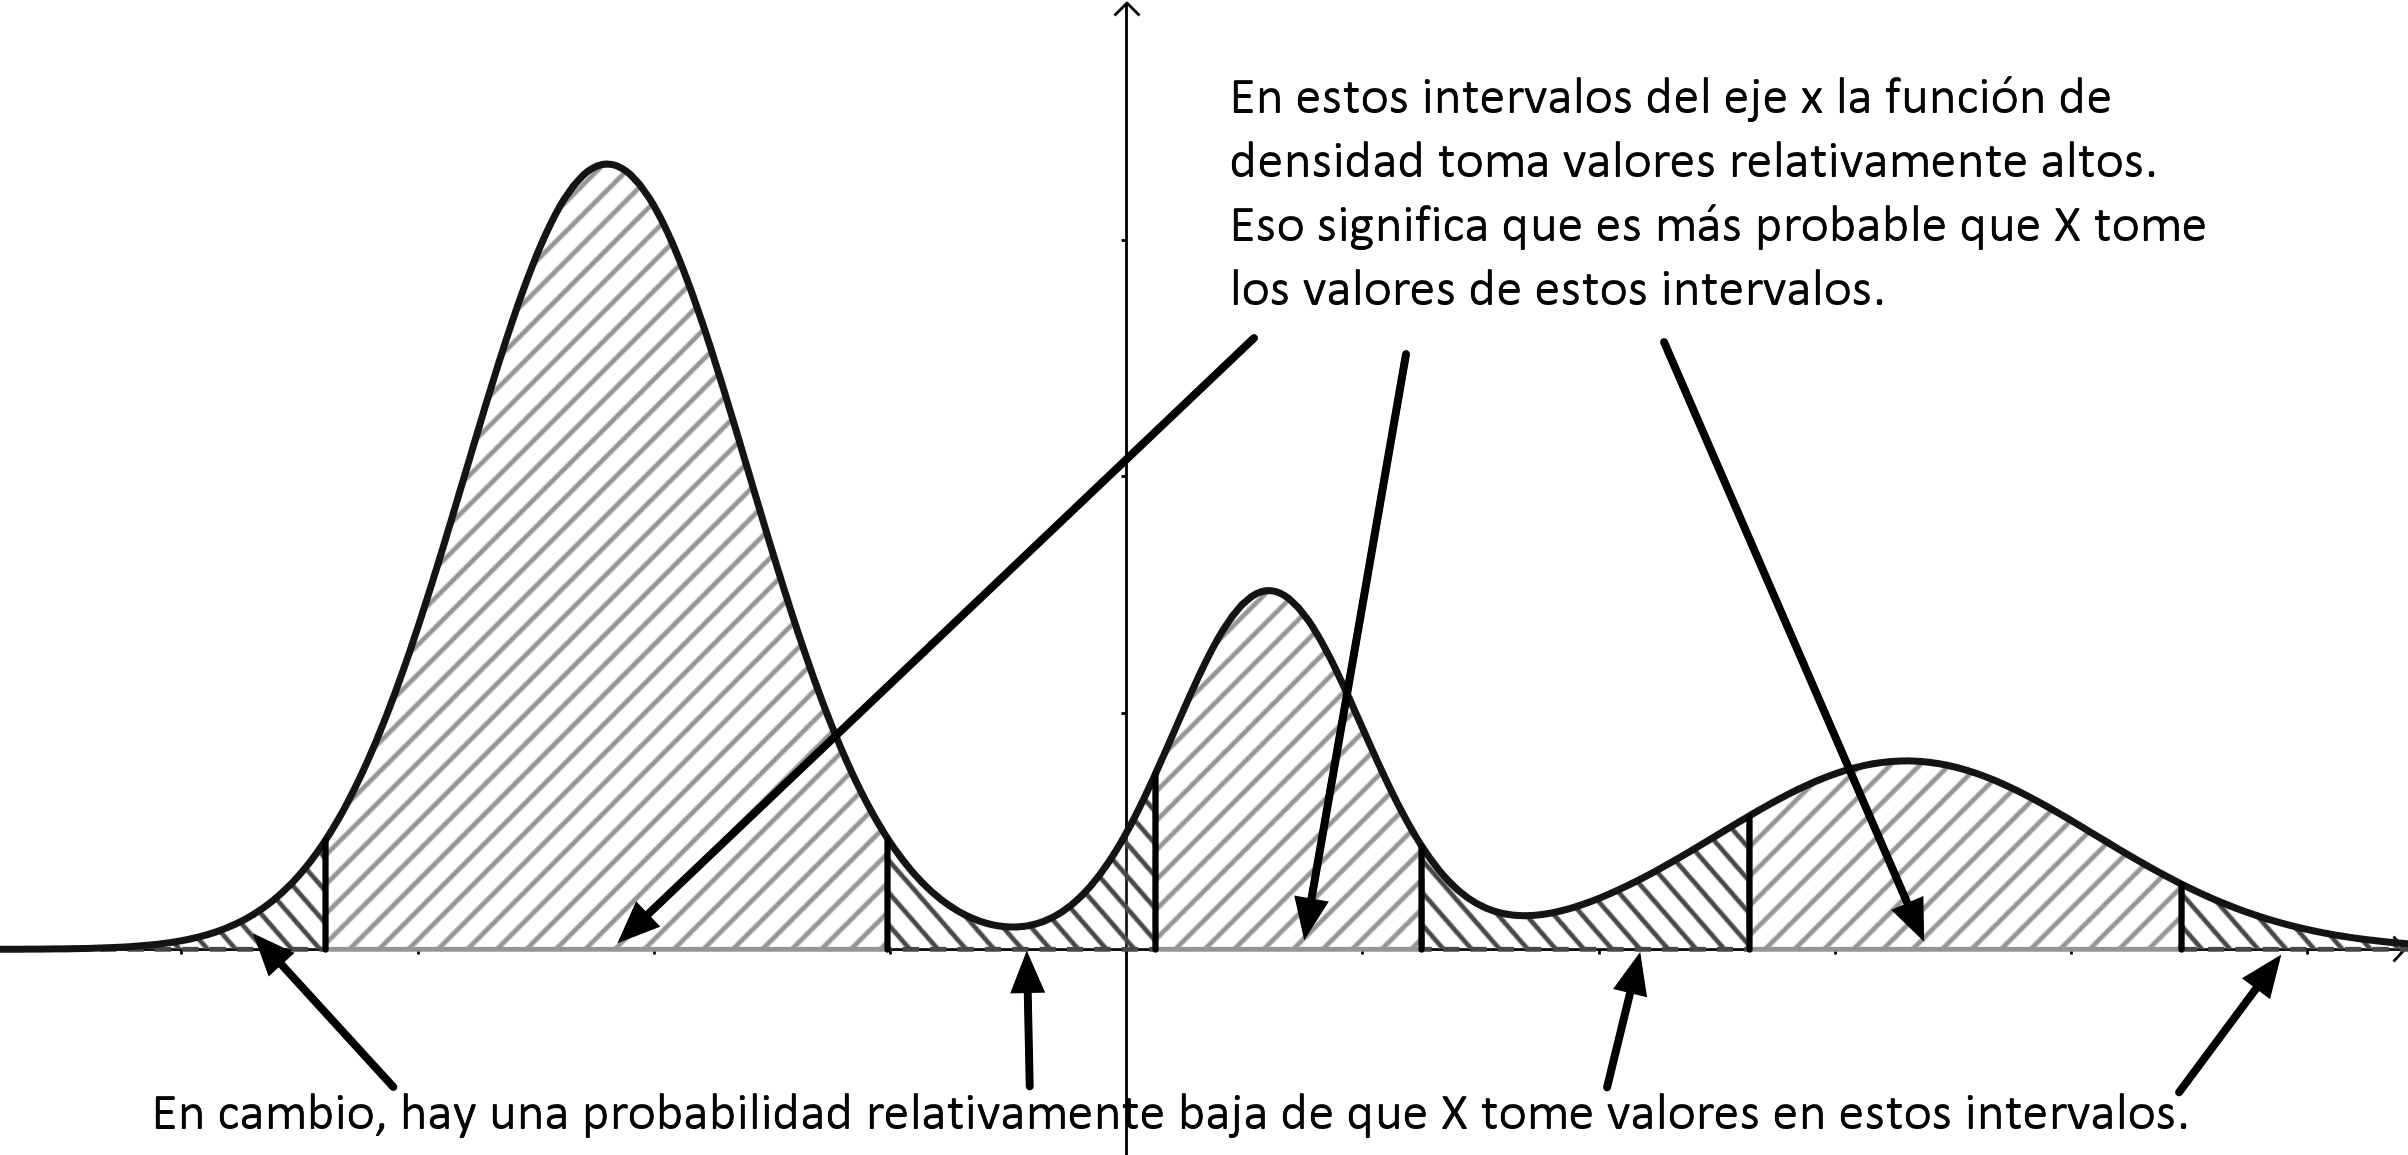
\includegraphics[width=12cm]{../fig/Cap05-InterpretacionFuncionDensidadFicticia-bn.png}
\end{bn}
\caption{La altura de la función de densidad indica los valores de $X$ con más probabilidad.}
\label{cap05:fig:Cap05-InterpretacionFuncionDensidadFicticia-bn.png}
\end{center}
\end{figure}

\subsection{Variables continuas con soporte en un intervalo.}
\label{cap05:subsec:VariablesContinuasSoporteIntervalo}

En el apartado precedente hemos trabajado con un ejemplo de función de densidad definida en $(-\infty, \infty)$. Es decir, que la variable aleatoria $X$ asociada con $f$ puede tomar todos los valores. Pero, como ya habíamos anunciado, en muchos otros casos, vamos a trabajar con variables continuas que sólo toman valores en un intervalo acotado $(a,b)$, o con casos intermedios, como las variables aleatorias que sólo toman valores positivos (es decir, en el intervalo $(0,+\infty)$).

Aunque al principio puede parecer que cada uno de esos casos es diferente, hay una forma en la que podemos simplificar las cosas, y tratar a todos los casos por igual. {\sf Basta con redefinir $f$, para que pase a valer $0$ en todos los valores en los que, originalmente, no estaba definida.} Al hacer esto no se modifica ninguna asignación de probabilidad, y lo que es más importante, si $f$ es $0$ fuera de un intervalo $(a,b)$, entonces da igual escribir las integrales usando ese intervalo o integrando desde $-\infty$ hasta $\infty$. En fórmulas:
    \begin{center}
    \fcolorbox{black}{Gris025}{
    \begin{minipage}{12cm}
        %%%%%%%%%%%%%%%%%%%%%%%%%%%%%%%%%%%%%%%
        Si $f$ vale $0$ fuera del intervalo $(a,b)$, entonces:
              \begin{equation}\label{cap05:ecu:INtegralFuncionesSoporteAcotado}
              \int_{-\infty}^{\infty}f(x)dx=\int_a^b f(x)dx
              \end{equation}
        %%%%%%%%%%%%%%%%%%%%%%%%%%%%%%%%%%%%%%%
    \end{minipage}}
    \end{center}
Esto, como vamos a ver enseguida, nos permite escribir muchas fórmulas teóricas usando $(-\infty,\infty)$, aunque luego, en la práctica, a veces sólo integraremos en intervalos en los que la función sea distinta de cero. Veamos un ejemplo.
\begin{ejemplo}
\label{cap05:ejem:FuncionDensidadSoporteFinito}
    Supongamos que $X$ es una variable aleatoria continua cuya función de densidad es
    \[f(x)=\begin{cases}6\cdot(x-x^2)&\mbox{ para }0\leq x\leq 1\\ 0&\mbox{en otro caso}\end{cases}\]
    como se ve en la Figura \ref{cap05:fig:InterpretacionFuncionDensidadSoporteFinito}.

\begin{figure}[htbp]
\begin{center}
\begin{enColor}
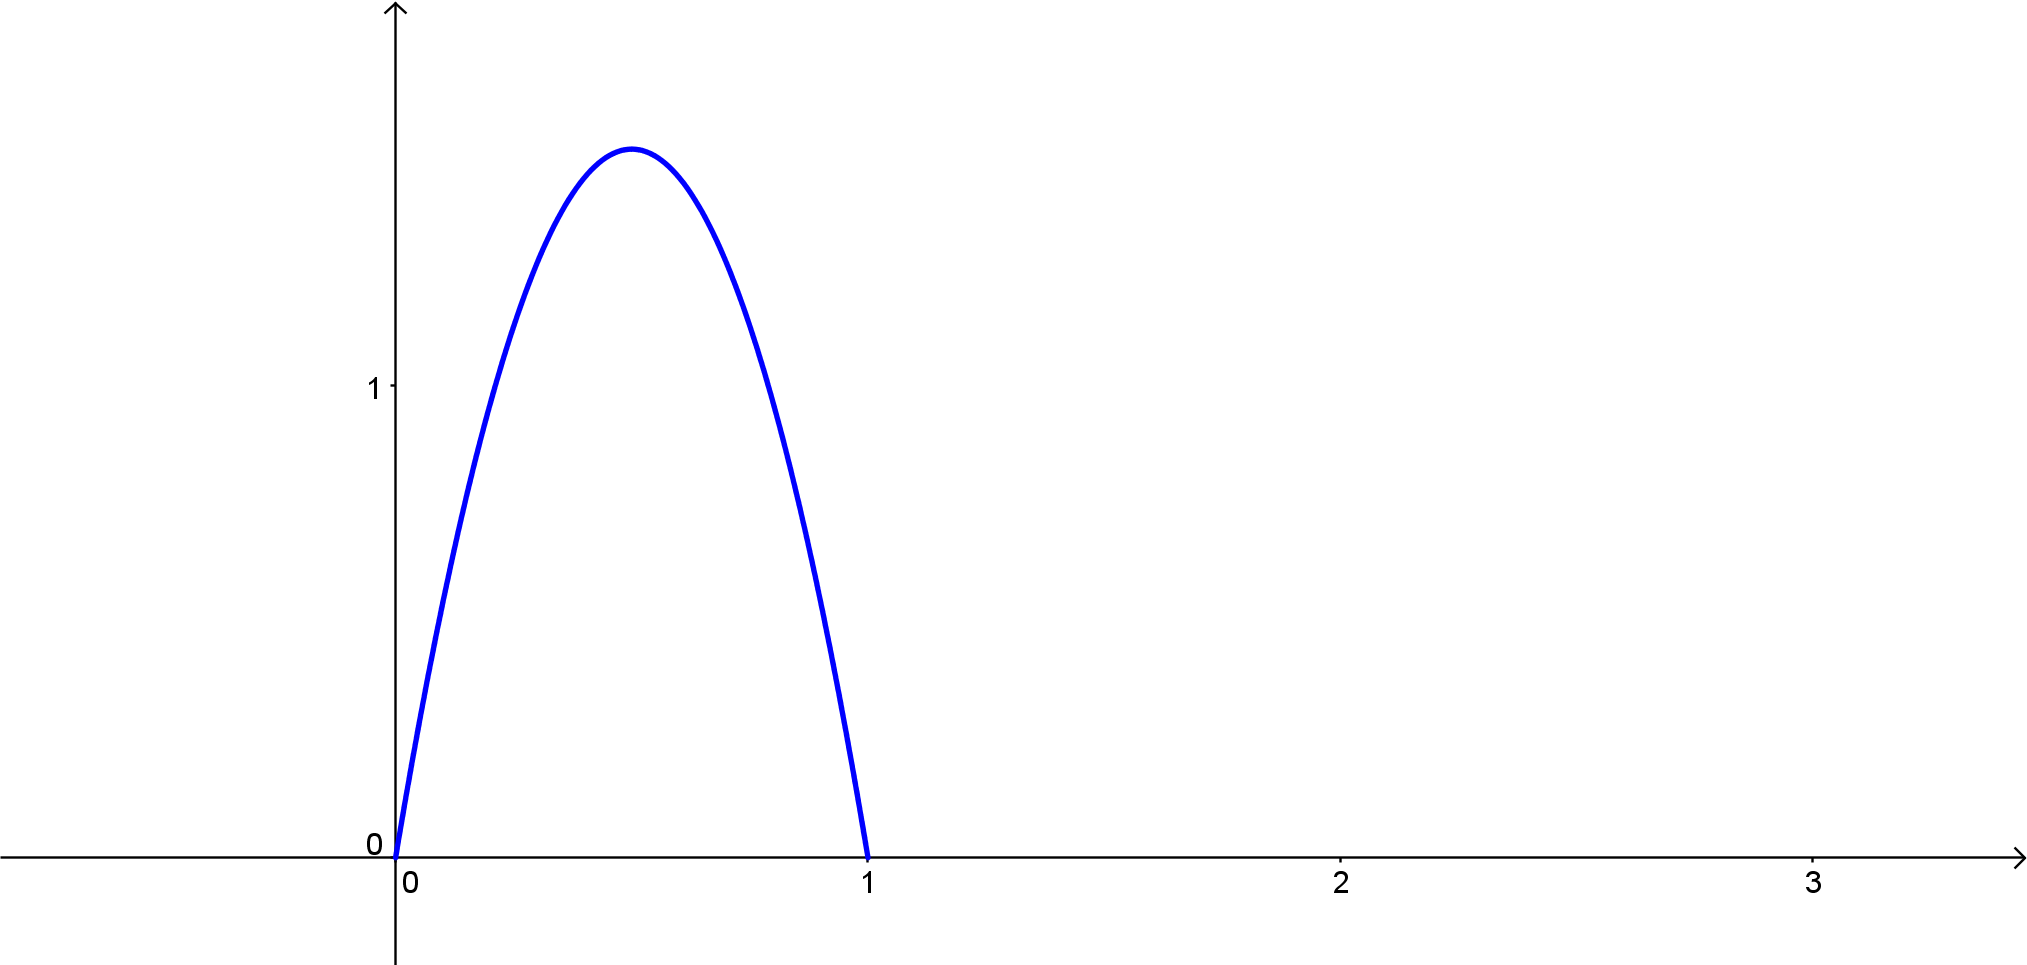
\includegraphics[width=12cm]{../fig/Cap05-InterpretacionFuncionDensidadSoporteFinito.png}
\end{enColor}
\begin{bn}
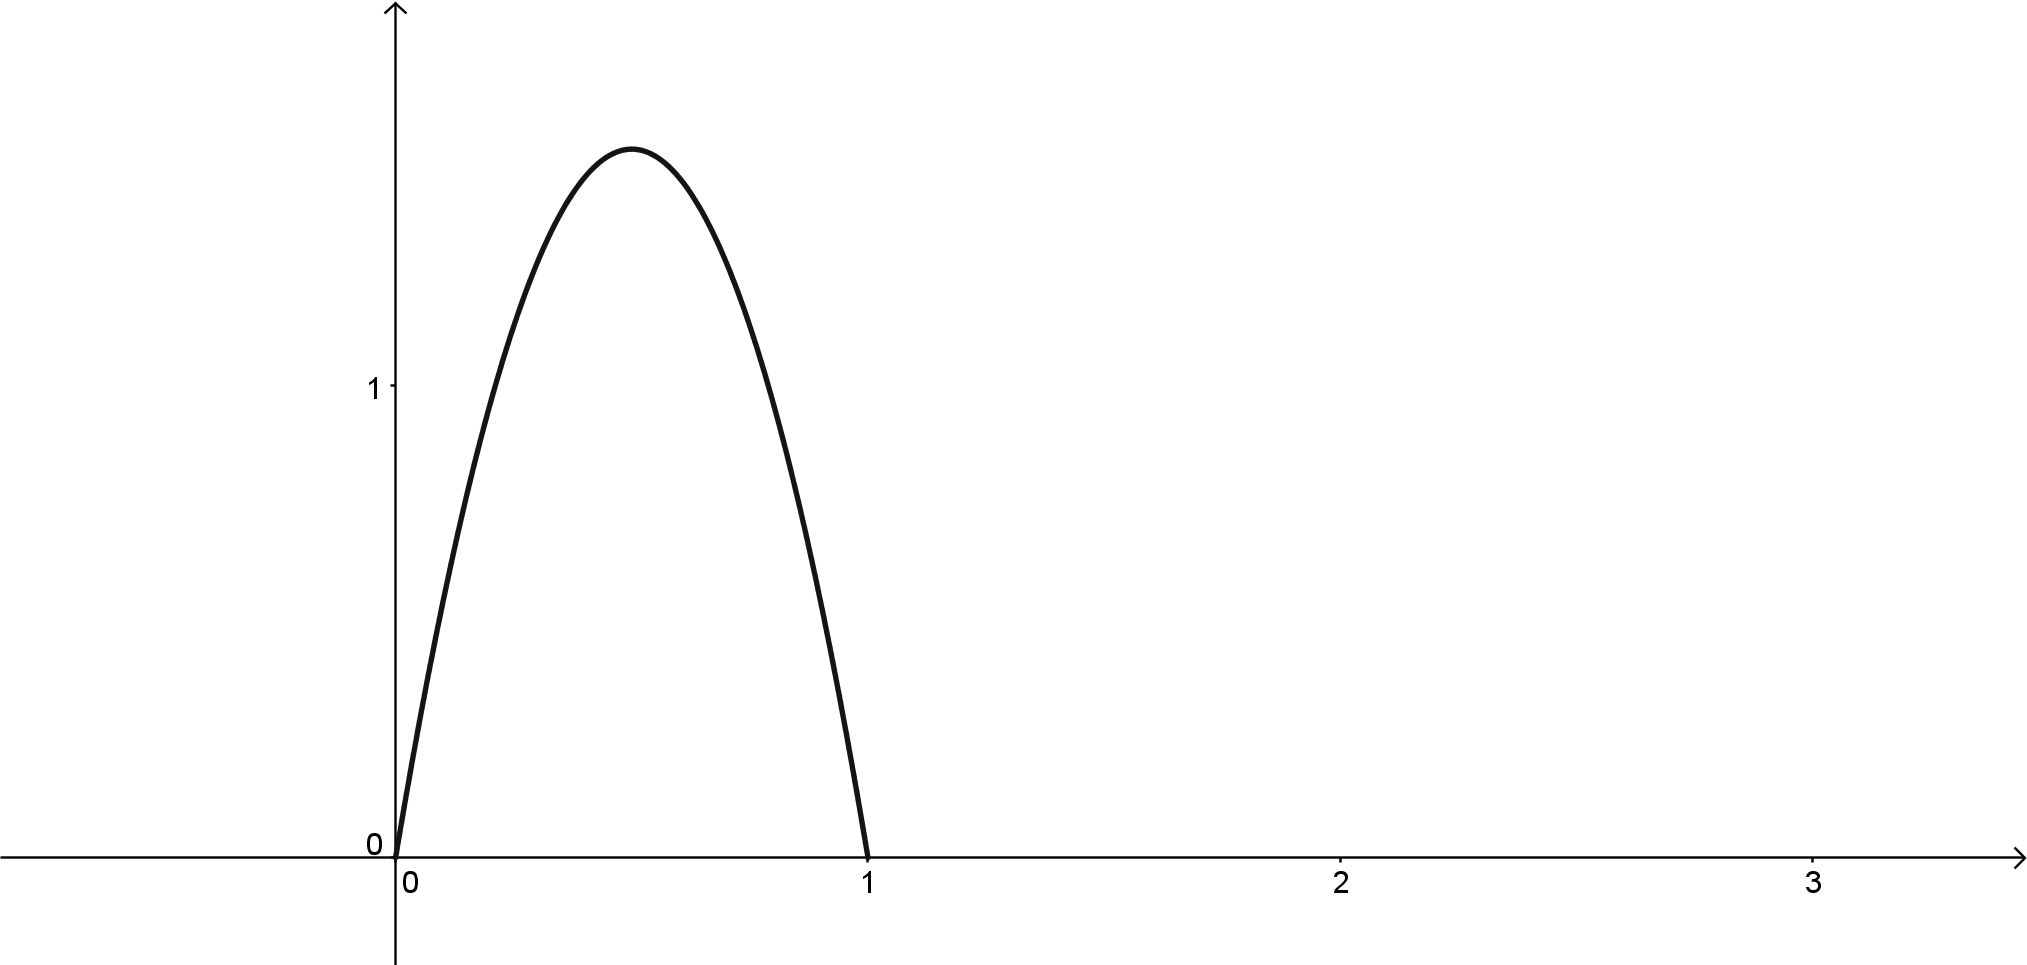
\includegraphics[width=12cm]{../fig/Cap05-InterpretacionFuncionDensidadSoporteFinito-bn.png}
\end{bn}
\caption{Una función de densidad que sólo es $\neq 0$ en $(0,1)$.}
\label{cap05:fig:InterpretacionFuncionDensidadSoporteFinito}
\end{center}
\end{figure}

    Dejamos como ejercicio para el lector (hacerlo tras terminar de leer el ejemplo), comprobar que  que el área total bajo la gráfica de $f$ es 1.  Nosotros vamos a calcular una probabilidad, concretamente:
    \[P(1/2<X<3/4),\]
    es decir, el área sombreada de la Figura \ref{cap05:fig:InterpretacionFuncionDensidadSoporteFinito2}.

\begin{figure}[htbp]
\begin{center}
\begin{enColor}
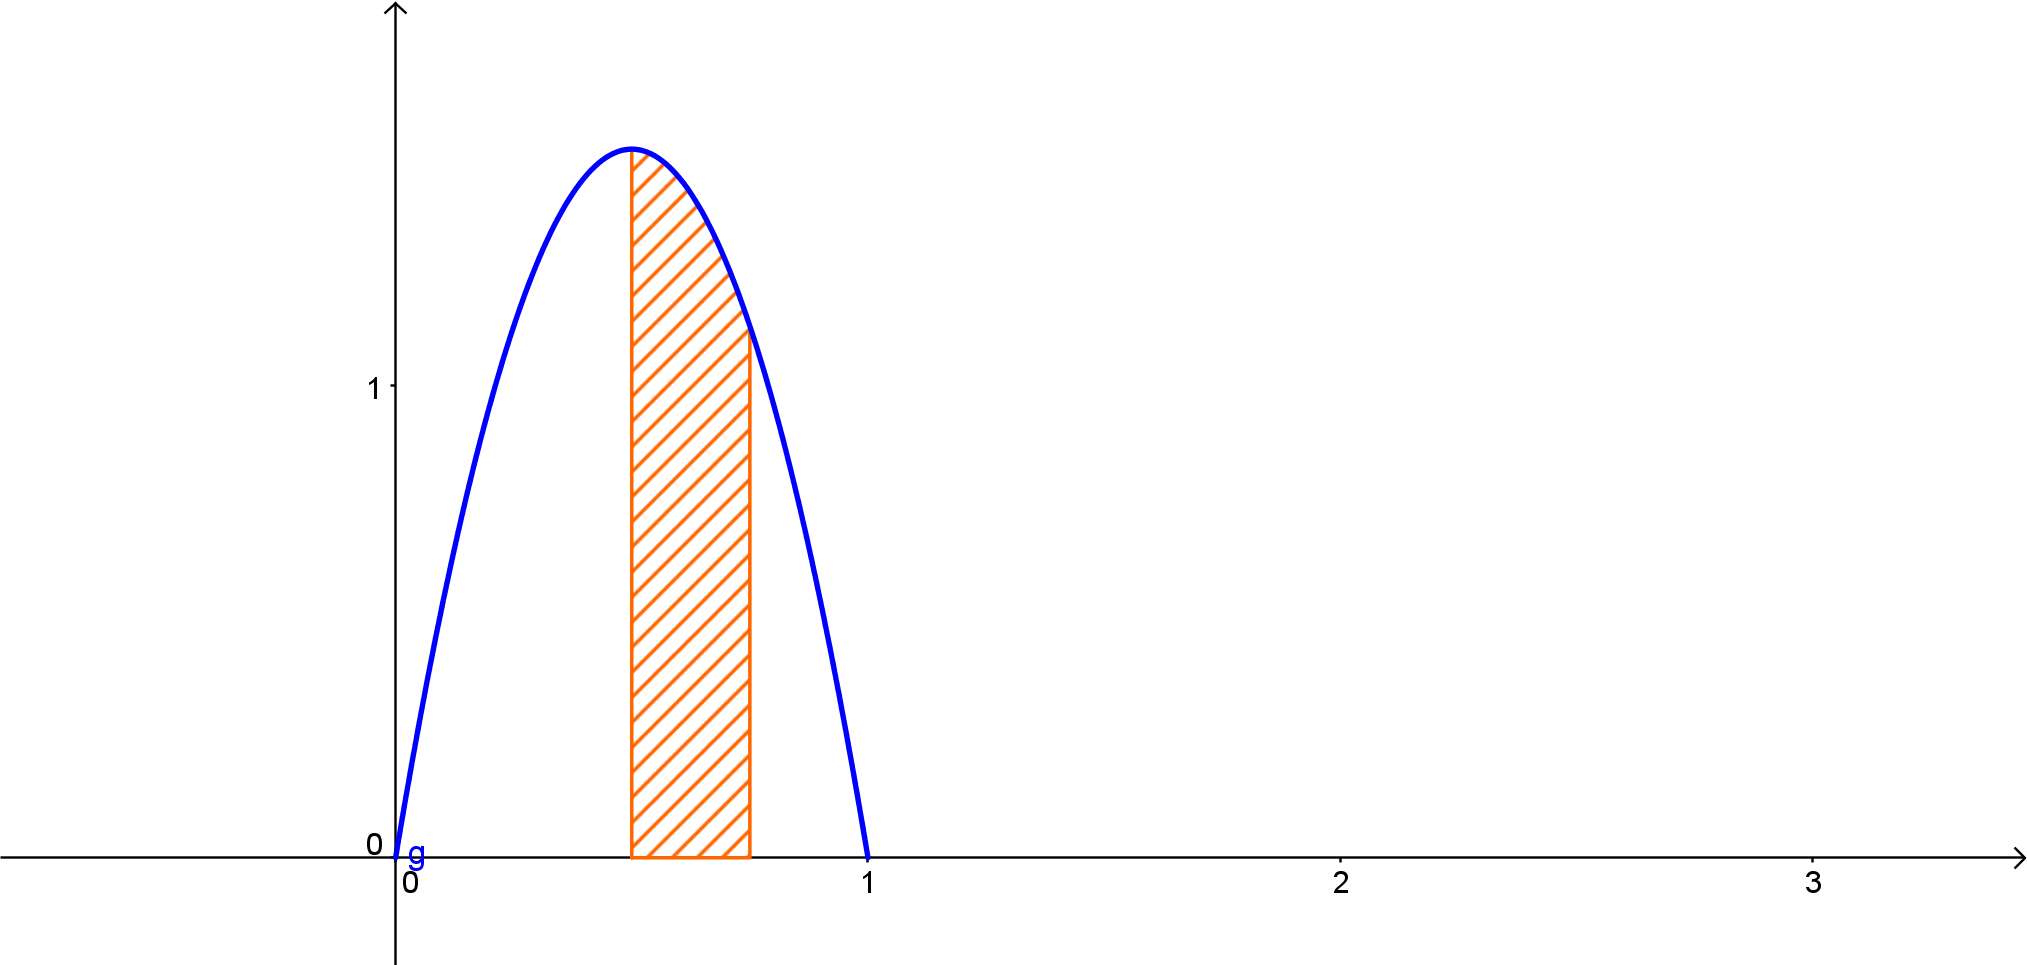
\includegraphics[width=12cm]{../fig/Cap05-InterpretacionFuncionDensidadSoporteFinito-2.png}
\end{enColor}
\begin{bn}
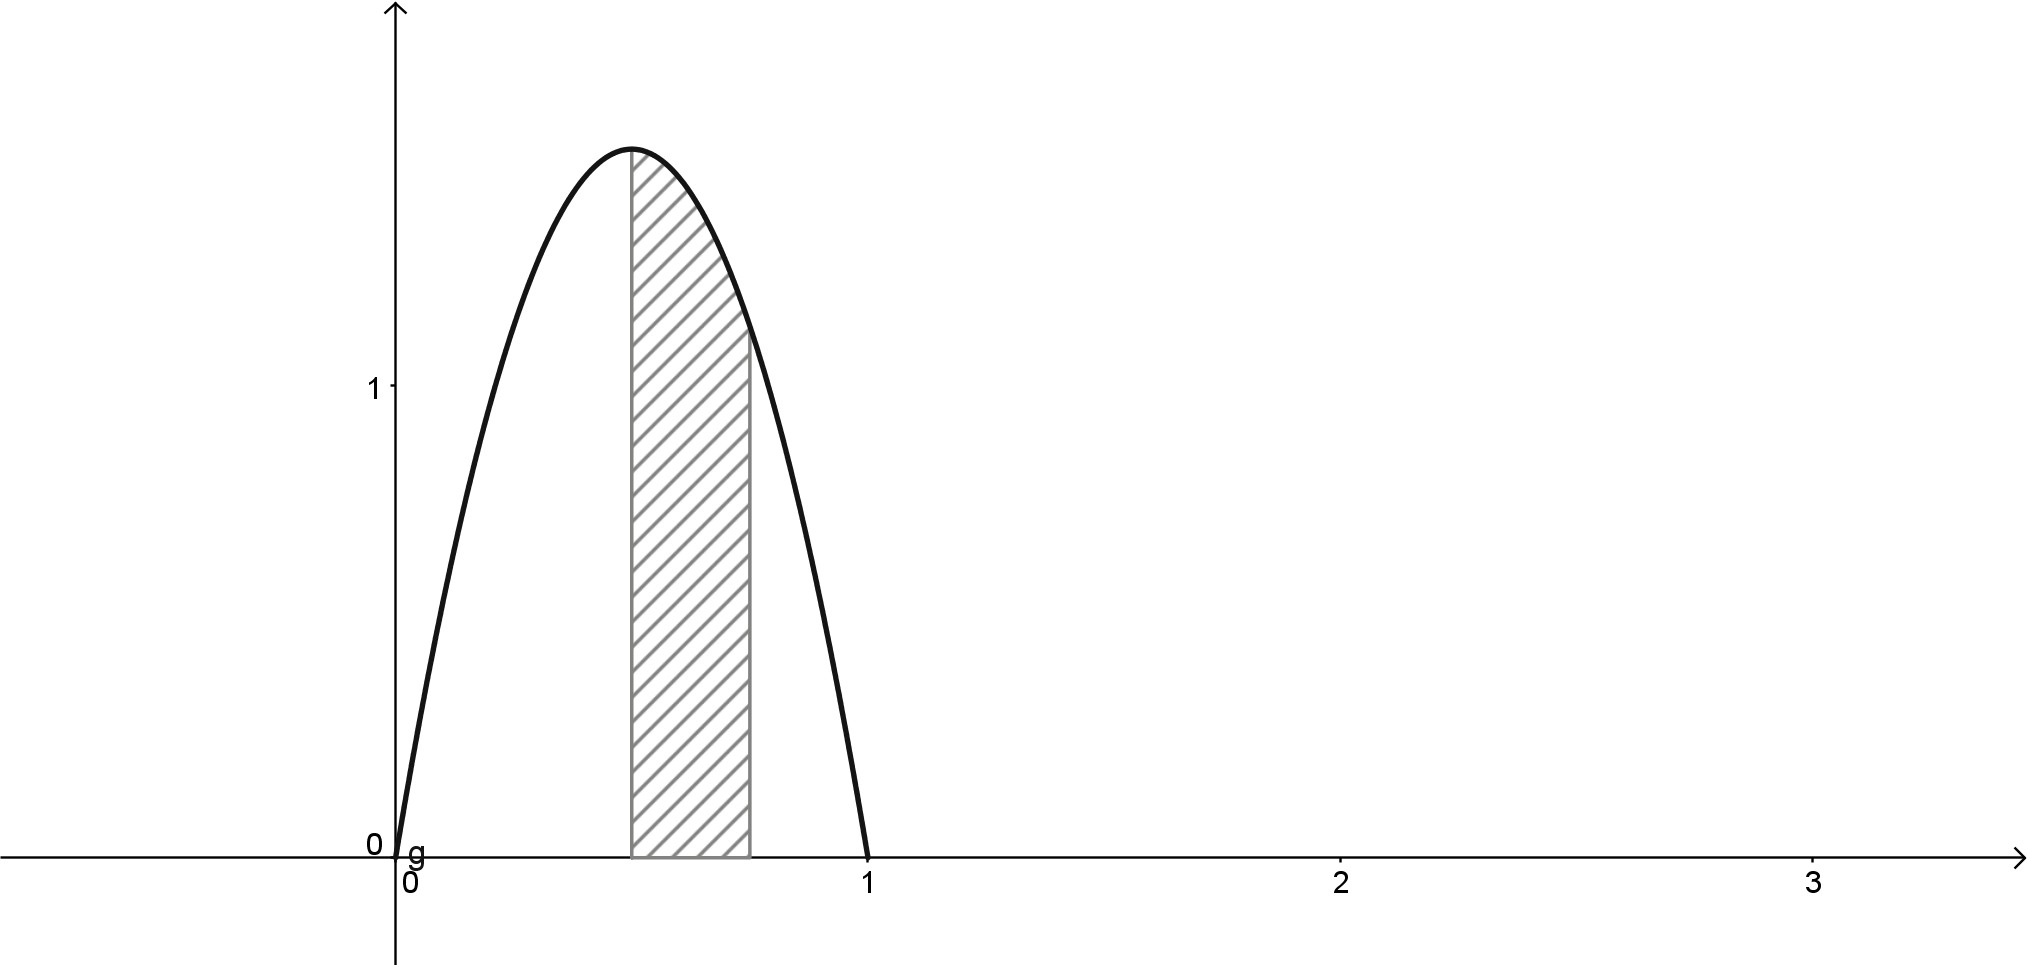
\includegraphics[width=12cm]{../fig/Cap05-InterpretacionFuncionDensidadSoporteFinito-2-bn.png}
\end{bn}
\caption{El área sombreada es $P\left(\frac{1}{2}<X<\frac{3}{4}\right)$}
\label{cap05:fig:InterpretacionFuncionDensidadSoporteFinito2}
\end{center}
\end{figure}

    Para calcularla tenemos que hallar el valor de la integral
    \[
    \int_{\frac{1}{2}}^{\frac{3}{4}} 6\cdot(x-x^2) dx
    \]
    Usando cualquiera de los programas que aparecen en el Tutorial05, podemos ver que el resultado es $\frac{11}{32}\approx 0.3438$. Una primitiva, por si el lector la necesita, es:
    \[F(x)=\begin{cases}(3 x^2-2 x^3)&\mbox{ para }0\leq x\leq 1\\ 0&\mbox{en otro caso}\end{cases}\]
    Lo que más nos interesa subrayar de este ejemplo es que, para calcular este valor de la probabilidad, nos ha dado igual que la función $f$ sólo esté definida en el intervalo $(0,1)$. El cálculo se hace exactamente igual en estos casos. \qed
\end{ejemplo}


Para cerrar este apartado, un poco de terminología: cuando la función de densidad de una variable aleatoria continua $X$ sólo es distinta de $0$ dentro de un cierto intervalo $(a,b)$, diremos que {\sf la variable $X$ tiene soporte en el intervalo $[a,b]$}\index{soporte de una función de densidad}. Así, la función del Ejemplo \ref{cap05:ejem:FuncionDensidadSoporteFinito} tiene soporte en el intervalo $(0,1)$.
%
%
%, si definimos una variable continua $X$ que representa la altura de los ciudadanos españoles, entonces los valores de $X$ (en cm) están todos ellos comprendidos en el intervalo $[0,300]$. En casos como este, los valores de $f(x)$ fuera del intervalo $[a,b]$ son iguales a cero . Y eso incluso simplifica nuestros cálculos de medias y varianzas, porque, en lugar de una integral $\int_{-\infty}^{\infty}$, lo que tenemos que calcular es una integral $\int_a^b$.

\subsection{Media y varianza de una variable aleatoria continua.}
\label{cap05:subsec:MediaVarianzaVariableAleatoriaContinua}

Es fácil entender que, al empezar el trabajo con las variables aleatorias continuas, uno de nuestros primeros objetivos sea extender la definición de media y varianza a este caso. Por tanto, si tenemos una variable aleatoria continua $X$, con función de densidad $f(x)$ (para fijar ideas, podemos pensar en un ejemplo como el de la Figura \ref{cap05:fig:Cap05-InterpretacionFuncionDensidadFicticia-bn.png}), ¿cómo definiríamos la media $\mu$ de esta variable?

Lo mejor que podemos hacer es volver a terreno conocido, en busca de inspiración. Los siguientes párrafos ni son, ni pretenden ser, una demostración. Al final, vamos a dar una definición de la media de un variable aleatoria continua. Pero antes, vamos a tratar de argumentar de dónde sale esa definición. Lo hacemos, entre otras cosas, porque creemos que es una parte muy valiosa de la formación científica del lector. Así que creemos que es muy conveniente que el lector se tome el tiempo de tratar de entender la siguiente discusión. Como siempre, sin agobios. Lo que no se entienda en una primera lectura, puede quedar más claro cuando avance el curso. En cualquier caso, la discusión terminará en la definición de media de la Ecuación \ref{cap05:ecu:mediaVariableAleatoriaContinua} (pág.\pageref{cap05:ecu:mediaVariableAleatoriaContinua}), por si el lector se pierde y decide reunirse con nosotros allí.


La discusión se puede ver como una continuación de la que tuvimos al final de la Sección \ref{sec:distribucionesContinuasEntranEscena}, sobre la interpretación de la integral como un límite de sumas. De hecho, ese es el papel fundamental que la integral juega muchas veces en la aplicaciones. Cuando tenemos un problema en un contexto continuo, a menudo tratamos de descomponerlo como suma (aproximada) de muchos problemas discretos. Y una vez resueltos esos problemas discretos, la solución del problema continuo es la integral de las soluciones discretas.

Para llegar a eso, empezamos recordando que, en el caso discreto (con un número finito de valores), el equivalente de la función de densidad es una tabla como la Tabla
\ref{cap05:tabla:tablaDensidadProbabilidadGenericaVariableAleatoriaDiscreta}. Y en ese caso definíamos la media así:
    \[\mu=\sum_{i=1}^{k}x_iP(X=x_i)=x_1 p_1+x_2 p_2+\cdots+x_k p_k.\]
    \begin{table}[h]
    \begin{center}
    \begin{tabular}[t]{|c|c|c|c|c|c|}
    \hline
    \rule{0cm}{0.5cm}{\em Valor:}&$x_1$&$x_2$&$x_3$&$\cdots$&$x_k$\\
    \hline
    \rule{0cm}{0.7cm}{\em Probabilidad:}&$p_1$&$p_2$&$p_3$&$\cdots$&$p_k$\\
    \hline
    \end{tabular}
    \end{center}
    \caption{Repetimos aquí la Tabla \ref{cap04:tabla:tablaDensidadProbabilidadGenericaVariableAleatoriaDiscreta} (pág \pageref{cap04:tabla:tablaDensidadProbabilidadGenericaVariableAleatoriaDiscreta})
    : densidad de probabilidad de una variable aleatoria discreta (con un número finito de valores)}\label{cap05:tabla:tablaDensidadProbabilidadGenericaVariableAleatoriaDiscreta}
    \end{table}

¿Cómo podemos extender esta definición de la media al caso de una variable continua con función de densidad $f(x)$? Bueno, siempre podemos {\em desandar el camino que tomó De Moivre}. Es decir, podemos pensar en reemplazar la función $f(x)$ por una (enorme) colección de rectángulos, como en la Figura \ref{cap05:fig:Discretizacion}.

\begin{figure}[htbp]
\begin{center}
\begin{enColor}
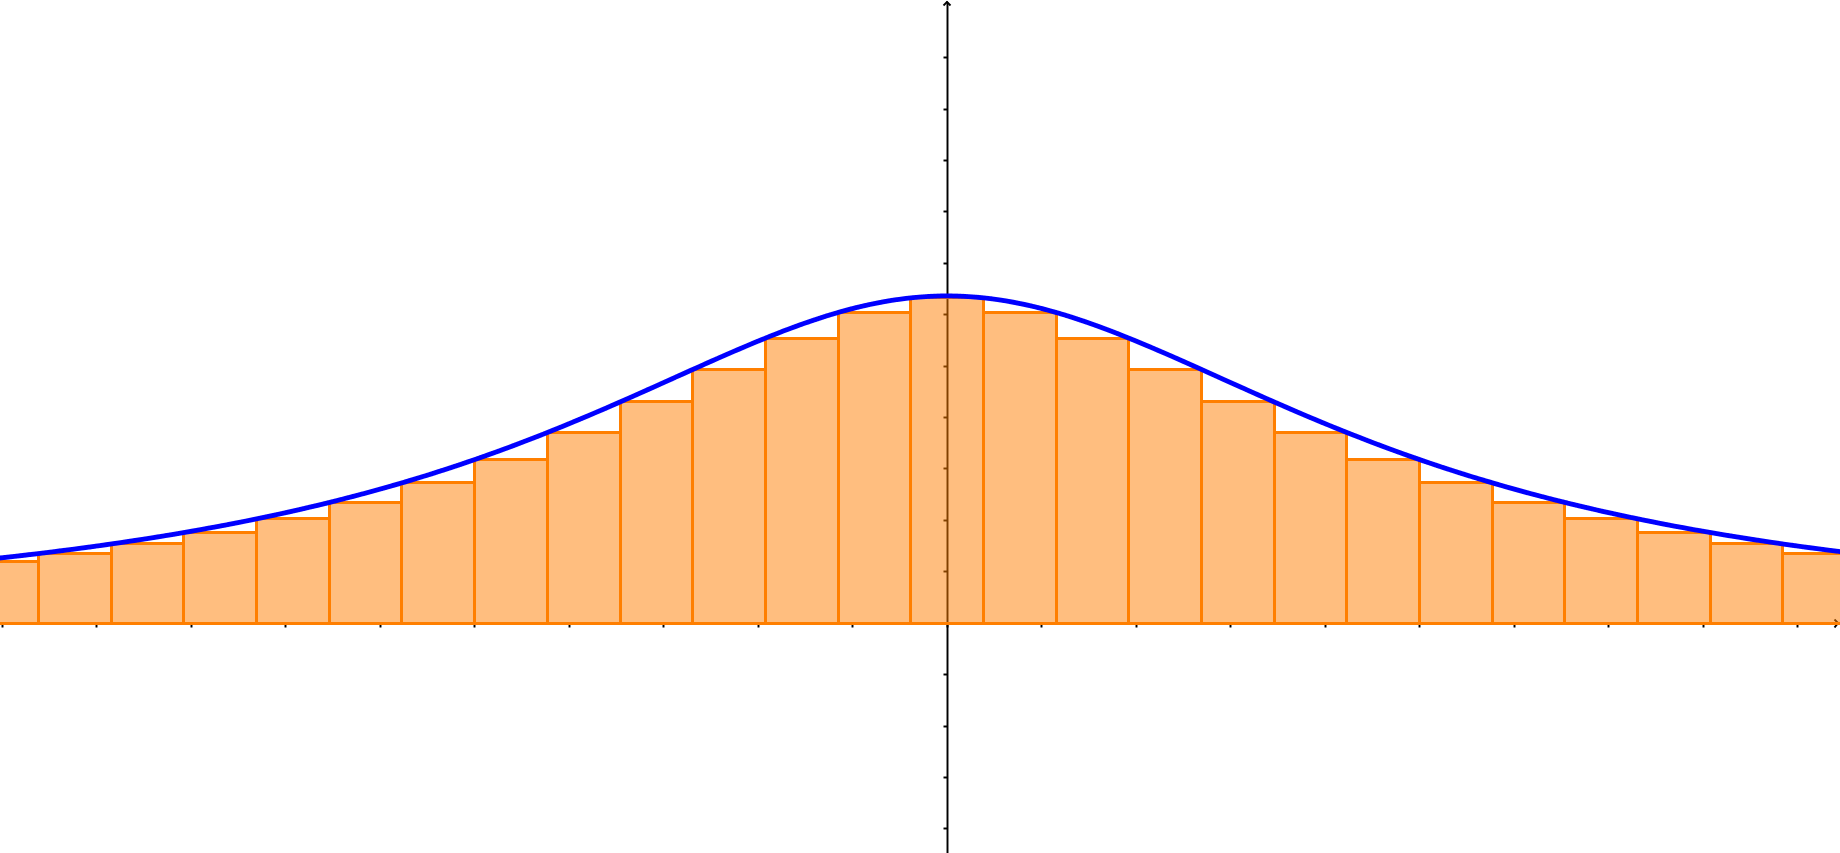
\includegraphics[width=12cm]{../fig/Cap05-Discretizacion.png}
\end{enColor}
\begin{bn}
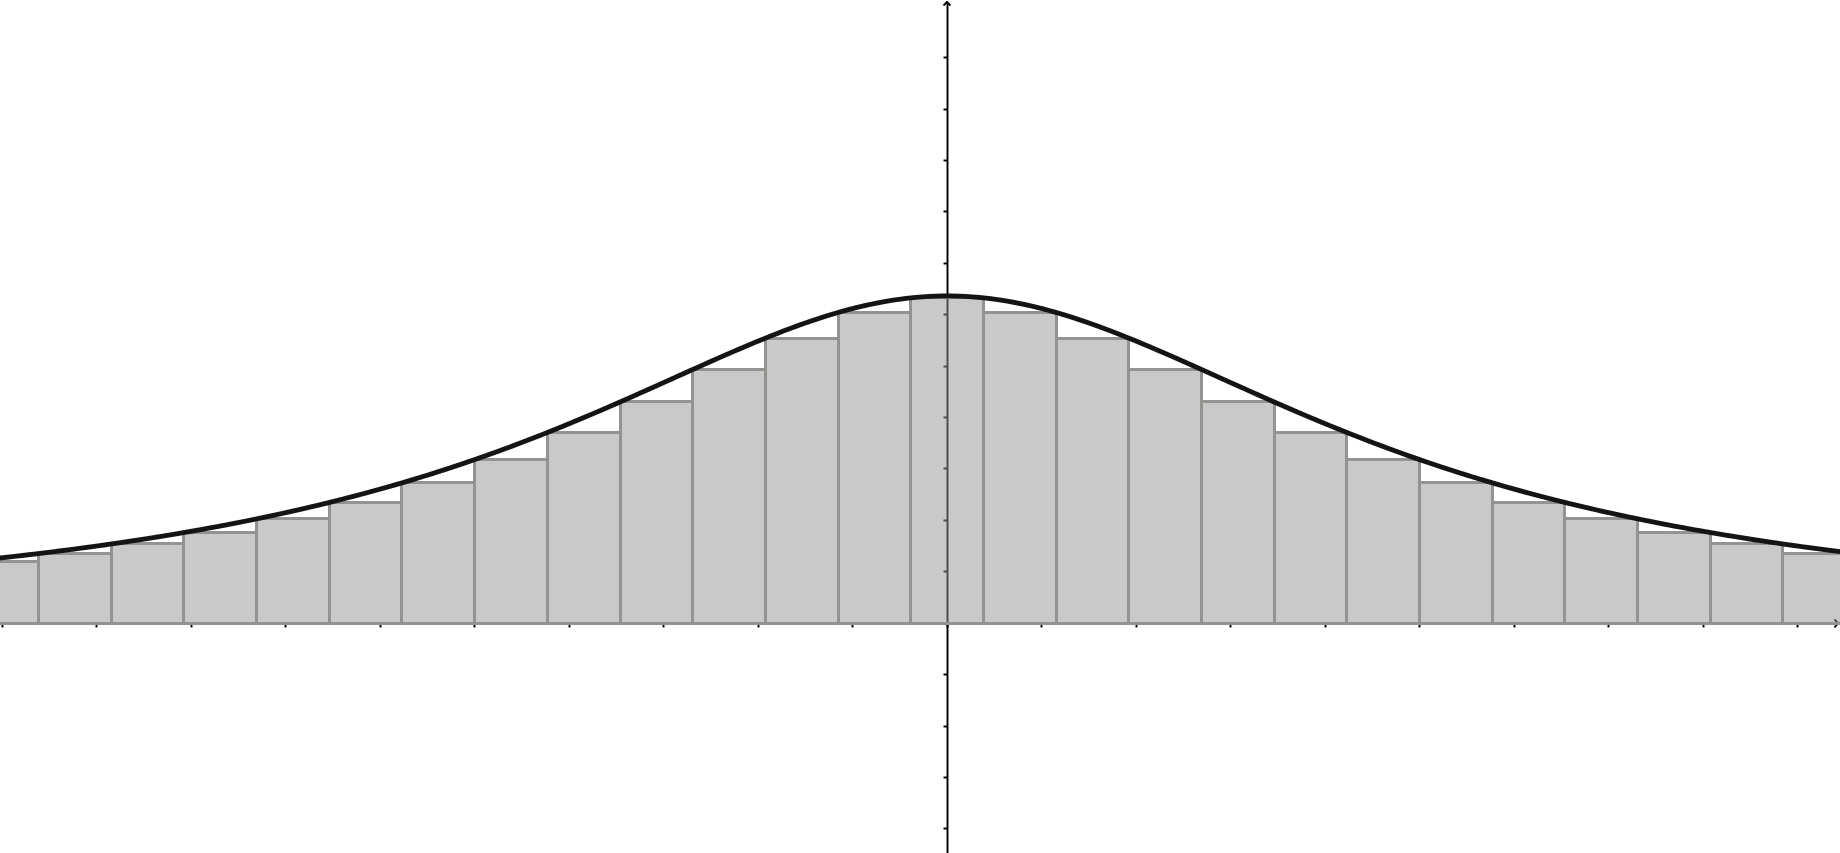
\includegraphics[width=12cm]{../fig/Cap05-Discretizacion-bn.png}
\end{bn}
\caption{Discretizando una variable aleatoria continua}
\label{cap05:fig:Discretizacion}
\end{center}
\end{figure}

A continuación podemos {\em ``olvidar''} la curva $f(x)$ y simplemente pensar en estos rectángulos, como si fueran el resultado de una tabla como la \ref{cap05:tabla:tablaDensidadProbabilidadGenericaVariableAleatoriaDiscreta}. Si tuviéramos delante esta tabla, ya sabemos que la media se calcularía haciendo:
   \begin{equation}\label{cap05:ecu:ArgumentacionMediaVariableContinua}
   \mu=E(X)\approx \sum_{\begin{minipage}{1.5cm}\tiny todos los\\ rectángulos\end{minipage}}x_i\cdot P(X=x_i)
   \end{equation}

La Figura \ref{cap05:fig:Discretizacion-detalle} pretende ilustrar los detalles de la siguiente discusión, en la que nos vamos a fijar en un intervalo concreto.

\begin{figure}[htbp]
\begin{center}
\begin{enColor}
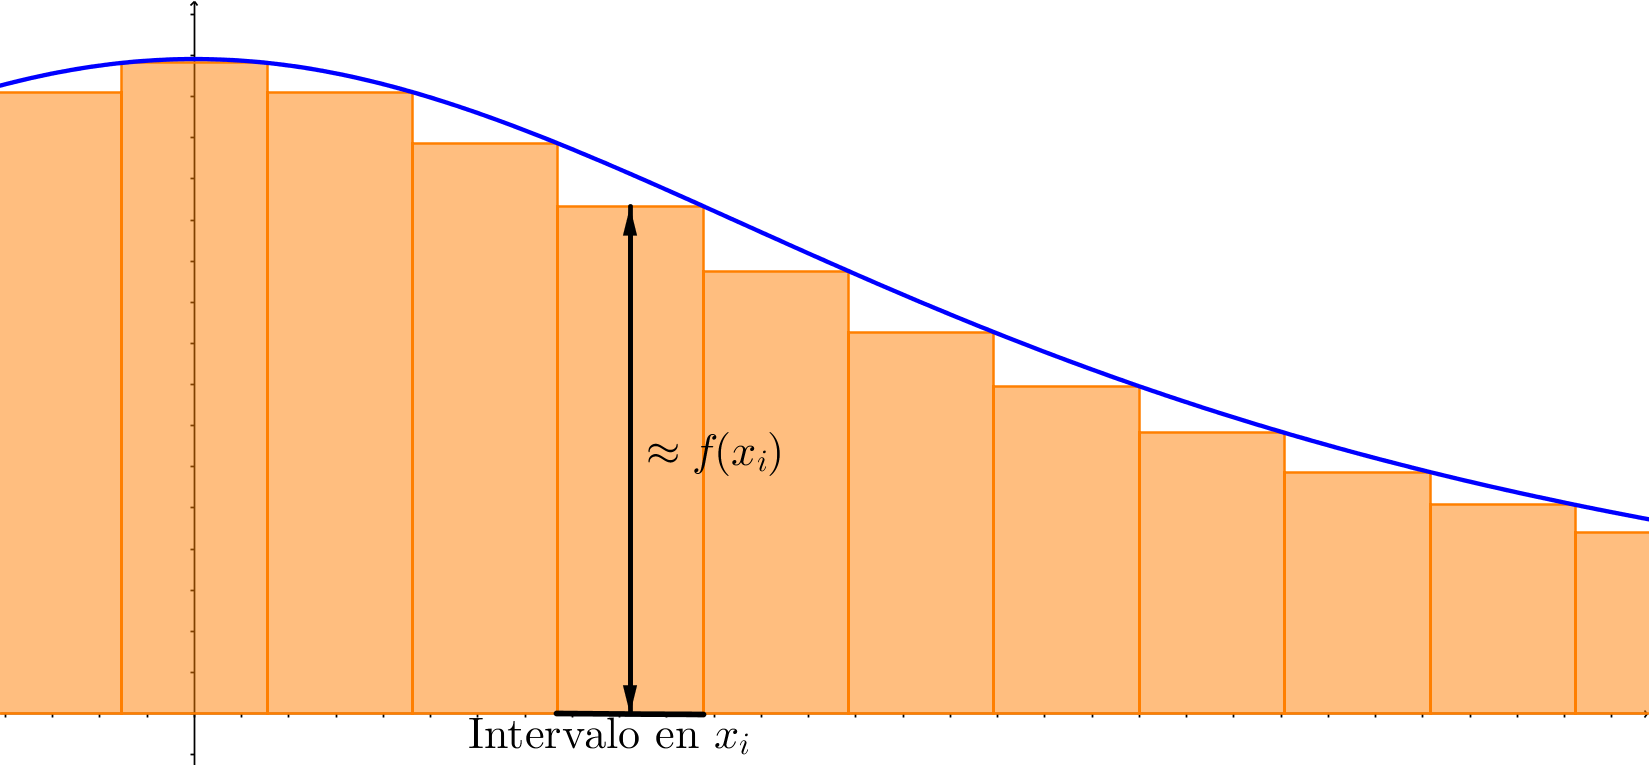
\includegraphics[width=12cm]{../fig/Cap05-Discretizacion-detalle.png}
\end{enColor}
\begin{bn}
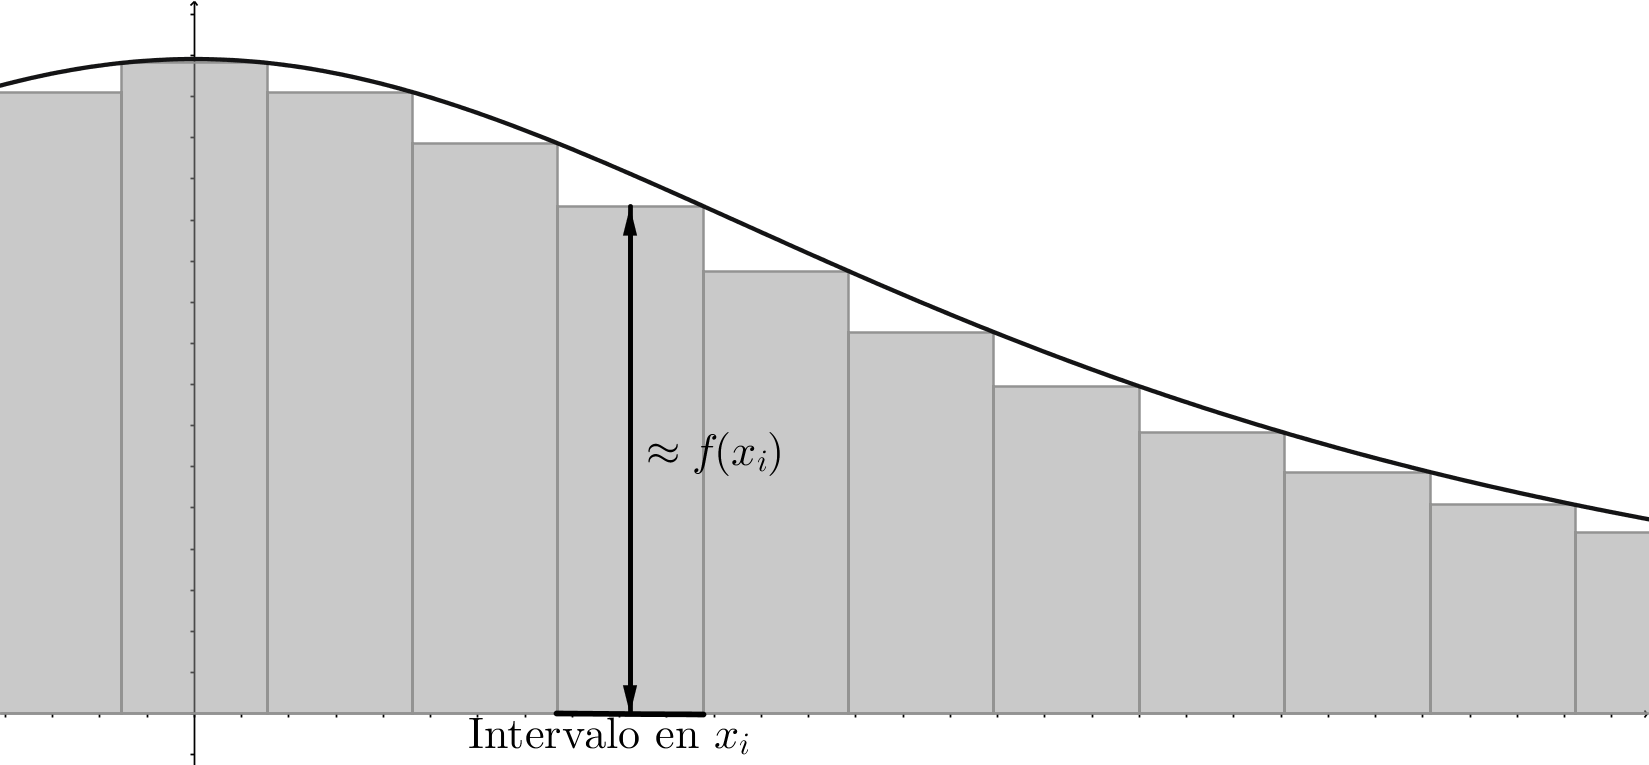
\includegraphics[width=12cm]{../fig/Cap05-Discretizacion-detalle-bn.png}
\end{bn}
\caption{Detalles de la discretización de una variable aleatoria continua}
\label{cap05:fig:Discretizacion-detalle}
\end{center}
\end{figure}

Pensemos un momento sobre los ingredientes de la suma en \ref{cap05:ecu:ArgumentacionMediaVariableContinua}: hay un sumando para cada uno de los rectángulos. Y cada rectángulo representa, {\em agrupándolos}, a todos  los valores de la variable $X$ que caen en ese intervalo. Este método, de agrupar todo un intervalo de valores de una variable continua, nos acompaña desde el Capítulo \ref{cap:IntroduccionEstadisticaDescriptiva} (ver la discusión de la pág. \pageref{cap01:tabla:FrecuenciaPesoClase}), cuando usábamos el punto medio de cada intervalo como {\em marca de clase}, para representar al resto de valores de ese intervalo. Por lo tanto, podemos pensar que el valor $x_i$ que aparece en la Ecuación \ref{cap05:ecu:ArgumentacionMediaVariableContinua} es la marca de clase del correspondiente intervalo. El valor $P(X=x_i)$ es el área de ese rectángulo. Que es, naturalmente,
\[\mbox{altura}\cdot\mbox{base}.\]
La altura del rectángulo, como apunta la Figura \ref{cap05:fig:Discretizacion-detalle}, vale aproximadamente $f(x_i)$. Podemos por tanto reescribir la suma como:
   \[\mu=E(X)\approx \sum_{\begin{minipage}{1.5cm}\tiny todos los\\ rectángulos\end{minipage}} x_i\cdot f(x_i)\cdot\mbox{(base del rectángulo)}.\]
Hemos escrito un símbolo de aproximación porque hemos sustituido la altura real de los rectángulos por $f(x_i)$, y eso introduce un cierto error. Pero ese error será tanto menor cuanto más numerosos y estrechos sean los rectángulos. La situación tiene todos los ingredientes típicos de la transformación de una suma en una integral, cambiando las bases de los rectángulos por $dx$. Esquemáticamente:
\begin{equation}\label{cap05:ecu:EsquemaMediaDiscretoAContinuo}
\begin{array}{ccccc}
\mbox{Mundo discreto: }\mu=&\displaystyle\sum_{\begin{minipage}{1.5cm}\tiny todos los\\ rectángulos\end{minipage}}& x_i f(x_i)&\cdot&\mbox{\small (bases rectángulos)}\\
&\left\downarrow\rule{0cm}{0.5cm}\right.&\left\downarrow\rule{0cm}{0.8cm}\right.&\quad &\left\downarrow\rule{0cm}{0.8cm}\right.\\[5mm]
\mbox{Mundo continuo: }\mu=&\displaystyle\int_{-\infty}^{\infty}&
x f(x)&&
dx
\end{array}
\end{equation}
Con esto, estamos listos para la definición:
    \begin{center}
    \fcolorbox{black}{Gris025}{
    \begin{minipage}{12cm}
        \begin{center}
        %%%%%%%%%%%%%%%%%%%%%%%%%%%%%%%%%%%%%%%
        {\bf  Media (o valor esperado) de una variable aleatoria continua}
        \end{center}
        \index{media de una variable aleatoria continua}
        \index{valor esperado de una variable aleatoria continuas}
        %%%%%%%%%%%%%%%%%%%%%%%%%%%%%%%%%%%%%%%
           Si $X$ es una variable aleatoria continua con función de densidad $f(x)$, entonces la {\sf media} de $X$ es el valor
           \begin{equation}\label{cap05:ecu:mediaVariableAleatoriaContinua}
           \mu=\int_{-\infty}^{\infty} x\cdot f(x)dx.
           \end{equation}
        %%%%%%%%%%%%%%%%%%%%%%%%%%%%%%%%%%%%%%%
    \end{minipage}}
    \end{center}

Antes de seguir adelante, vamos a hacer algunas observaciones sobre esta definición:
\begin{itemize}
  \item Uno de los errores más frecuentes que cometen los principiantes es olvidar la $x$ que aparece dentro de la integral. Vamos a insistir: la media se calcula con:
           \[
           \mu=\int_{-\infty}^{\infty} \colorbox{lightgrey}{\large$\mathbf x$}\cdot f(x)dx.
           \]
      Si no ponemos la $x$, y escribimos
           \[
           \int_{-\infty}^{\infty} f(x)dx.
           \]

      al integrar $f$ en solitario estamos calculando una probabilidad. Y de hecho, en este caso, al integrar sobre todos los valores estamos calculando la probabilidad total, y siempre obtendríamos 1.

  \item Si la función de densidad tiene soporte en $(a,b)$ (recuerda: eso significa que es $0$ fuera de $(a,b)$), entonces de hecho la media se calcula con:
           \[
           \mu=\int_{\colorbox{lightgrey}{\large$\mathbf a$}}^{\colorbox{lightgrey}{\large$\mathbf b$}} x\cdot f(x)dx.
           \]
      porque la integral fuera de ese intervalo es $0$.
  \item En el Tutorial05 veremos como utilizar el ordenador para hacer estos ejemplos. Los cálculos son similares a los que hacíamos para calcular probabilidades. Sólo es preciso no olvidarse de la $x$ delante de $f(x)$.
\end{itemize}
Ahora que ya nos hemos ocupado de la media, la varianza resultará muy sencilla. Dejamos que el lector piense unos momentos sobre este esquema,
\begin{equation}\label{cap05:ecu:EsquemaVarianzaDiscretoAContinuo}
\begin{array}{ccccc}
\mbox{Mundo discreto: }\sigma^2=&\displaystyle\sum& (x_i-\mu)^2& P(X=x_i)\\
&&\left\downarrow\rule{0cm}{0.8cm}\right.&\\[5mm]
\mbox{Mundo continuo: }\sigma^2=&\displaystyle\int_{-\infty}^{\infty}&
\mbox{\large ??}&dx
\end{array}
\end{equation}
Antes de leer la definición:
    \begin{center}
    \fcolorbox{black}{Gris025}{
    \begin{minipage}{12.5cm}
        \begin{center}
        %%%%%%%%%%%%%%%%%%%%%%%%%%%%%%%%%%%%%%%
        {\bf  Varianza y desviación típica de una variable aleatoria continua}
        \end{center}
        \index{varianza de una variable aleatoria continua}
        \index{desviación típica de una variable aleatoria continuas}
       %%%%%%%%%%%%%%%%%%%%%%%%%%%%%%%%%%%%%%%
       Si $X$ es una variable aleatoria continua con función de densidad $f(x)$, entonces la {\sf varianza} de $f$ es el valor
       \begin{equation}\label{cap05:ecu:varianzaVariableAleatoriaContinua}
       \sigma^2=\int_{-\infty}^{\infty} (x-\mu)^2\cdot f(x)dx.
       \end{equation}
       Y. como de costumbre, la {\sf desviación típica} $\sigma$ es la raíz cuadrada de la varianza.
        %%%%%%%%%%%%%%%%%%%%%%%%%%%%%%%%%%%%%%%
    \end{minipage}}
    \end{center}
La Tabla \ref{cap05:tablas:MuSigmaFormulasDosTiposVariables} resume la situación para variables aleatorias discretas y continuas.
\begin{table}[h]
    \begin{center}
    \begin{tabular}{|l|c|c|}
    \hline
                        & $X$ Var. discreta& $X$ Var. continua                                                                            \\
    \hline
    Media $\mu$\rule{0cm}{1cm}& $\displaystyle\sum_{i=1}^k x_iP(X=x_i)$         & $\displaystyle \int_{-\infty}^{\infty} x\cdot f(x)dx$         \\
    &&\\
    \hline
    Varianza $\sigma^2$ \rule{0cm}{1cm}& $\displaystyle\sum_{i=1}^k (x_i-\mu)^2P(X=x_i)$ & $\displaystyle \int_{-\infty}^{\infty} (x-\mu)^2\cdot f(x)dx$ \\
    &&\\
    \hline
    \end{tabular}
    \end{center}
\caption{$\mu$ y $\sigma$ en variables aleatorias discretas y continuas}
\label{cap05:tablas:MuSigmaFormulasDosTiposVariables}
\end{table}

Como puede apreciarse, si se reemplaza $P(X=x_i)$ por $f(x)$, el paralelismo entre las dos fórmulas resulta evidente.

\begin{ejemplo}
\label{cap05:ejem:MediaVarianzaVariableAleatoriaContinua}
    Sea $X$ una variable aleatoria continua, con soporte en el intervalo $(1,2)$, cuya función de densidad es:
    \[
    f(x)=\begin{cases}2\cdot(2-x),&\mbox{ si }1<x<2.\\0,&\mbox{en otro caso.}\end{cases}
    \]
    ¿Cuál es la media de $X$? Tenemos que calcular:
    \[
    \mu=\int_{1}^{2}\colorbox{lightgrey}{\large$x$}f(x)dx=\int_{1}^{2}x\cdot 2\cdot(2-x)dx=2\int_{1}^{2}(2x-x^2)dx=2\left[x^2-\frac{x^3}{3}\right]_1^2=\]
    \[2\left(4-\frac{8}{3}\right)-2\left(1-\frac{1}{3}\right)=\dfrac{4}{3}\approx 1.333. \]
    Dejamos como ejercicio para el lector comprobar que la varianza es:
    \[
    \sigma^2=\int_{1}^{2}(x-\mu)^2f(x)dx=2\int_{1}^{2}\left(x-\dfrac{4}{3}\right)^2(2-x)dx=\dfrac{1}{18}\approx 0.05556.
    \]
    \qed
\end{ejemplo}

\subsection{La distribución uniforme.}
\label{cap05:subsec:DistribucionUniforme}

Hay un tipo especial de variables aleatorias continuas, que son, en algún sentido, las más sencillas de todas. La idea es fácil de entender, incluso engañosamente fácil. A menudo, para definir estas variables, que vamos a llamar {\em uniformes},  se dice, simplificando, que dado  un intervalo $(a,b)$, lo que queremos es que ``todos los puntos del intervalo sean igual de probables''. Pero ya sabemos que, en una distribución continua, la probabilidad de cualquier punto es cero, sea cual sea la distribución. Seguramente el lector se habrá dado cuenta de que estamos empezando a repetir la misma discusión que tuvimos al hablar de probabilidad geométrica en el Capítulo \ref{cap:Probabilidad}. Tenemos que reformular lo que queremos de otra manera, y la forma de hacerlo es diciendo que la probabilidad se reparte por igual a lo largo de todo el intervalo $(a,b)$. Más precisamente, la condición de equiprobabilidad realmente significa que la probabilidad de un subintervalo de $(a,b)$ sólo debería depender de su longitud, y no de su posición dentro de $(a,b)$. ¿Cómo debería ser su función de densidad para que se cumpla esto? En primer lugar, se trata de una función con soporte en $(a,b)$, en el sentido del apartado \ref{cap05:subsec:VariablesContinuasSoporteIntervalo} (pág. \pageref{cap05:subsec:VariablesContinuasSoporteIntervalo}). Además, al comentar la Figura \ref{cap05:fig:Cap05-InterpretacionFuncionDensidadFicticia-bn.png} (pág. \pageref{cap05:fig:Cap05-InterpretacionFuncionDensidadFicticia-bn.png}), hemos dicho que la probabilidad es mayor donde la función de densidad es más alta. Si todas las zonas de $(a,b)$ tienen que tener la misma probabilidad, entonces la función de densidad tiene que tener la misma altura en todas partes; es decir, tiene que ser constante. En primera aproximación, debe ser
\[
f(x)=\begin{cases}
k&\mbox{ si }a<x<b\\
0&\mbox{ en otro caso. }
\end{cases}
\]
Y ahora ya sabemos lo que viene a continuación: como la probabilidad total tiene que ser uno, podemos usar eso para determinar la constante $k$. La cuenta es esta:
\[
1=\int_a^b k dx
\]
Tenemos que encontrar una primitiva de la función constante $f(x)=k$. Esa primitiva es $F(x)=k\cdot x$, como puedes comprobar fácilmente derivando. También puedes usar un programa de integración simbólica, como hemos hecho en otros ejemplos. Pero en este caso es muy importante ser cuidadosos, y asegurarnos de que el programa entiende que la variable de la función es $x$ y no $k$. Veremos esto con más detalle en el Tutorial05.

Usando esa primitiva:
\[
1=\int_a^b k dx=F(b)-F(a)=k\cdot b-k\cdot a=k\cdot(b-a)
\]
Y despejando, obtenemos $k=\dfrac{1}{b-a}$. Pongamos todas las piezas juntas:
    \begin{center}
    \fcolorbox{black}{Gris025}{
    \begin{minipage}{12cm}
        \begin{center}
        %%%%%%%%%%%%%%%%%%%%%%%%%%%%%%%%%%%%%%%
        {\bf Distribución uniforme en $(a,b)$}
        \index{distribución uniforme}\index{uniforme, distribución}
        \end{center}
        %%%%%%%%%%%%%%%%%%%%%%%%%%%%%%%%%%%%%%%
        Una variable aleatoria continua es de tipo {\sf uniforme} en el intervalo $(a,b)$ si su función de densidad es de la forma:
            \begin{equation}
            \label{cap05:ecu:DensidadUniforme}
            f(x)=\begin{cases}
            \dfrac{1}{b-a}&\mbox{ si }a<x<b\\[3mm]
            0&\mbox{ en otro caso. }
            \end{cases}
            \end{equation}
        En ese caso, la probabilidad de cualquier subintervalo de $(a,b)$ es proporcional a su longitud. Es decir, si el intervalo $(c,d)$ está contenido por completo dentro del $(a,b)$, se cumple que:
        \begin{equation}
        \label{cap05:ecu:ProbabilidadSubintervaloUniforme}
        P(c < X < d)=\dfrac{(d-c)}{b-a}.
        \end{equation}
        %%%%%%%%%%%%%%%%%%%%%%%%%%%%%%%%%%%%%%%
    \end{minipage}}
    \end{center}


\section{Función de distribución y cuantiles de una variable aleatoria continua.}
\label{cap05:sec:FuncionDistribucionVariableContinua}

En la página \pageref{cap04:ecu:FuncionDistribucionVariableDiscreta} hemos visto la definición de función de distribución de una  variable aleatoria discreta $X$, que era:
\[F(x)=P(X\leq x),\mbox{ para cualquier número real }x.\]
Dijimos en aquel momento que si la función (o tabla)de densidad $f(x)$ se corresponde con una tabla de valores de $X$ y sus probabilidades (ver la Tabla \ref{cap04:tabla:tablaDensidadProbabilidadGenericaVariableAleatoriaDiscreta}, pág.
\pageref{cap04:tabla:tablaDensidadProbabilidadGenericaVariableAleatoriaDiscreta}), entonces la función de distribución $F(x)$ se obtiene simplemente acumulando los valores de probabilidad de esa tabla.

Pero si observamos la definición anterior de $F$, veremos que no hay nada en esa definición que obligue a imponer la condición de que $X$ sea discreta. Lo único que dice la definición de $F(X)$ es que tenemos que calcular la probabilidad de que $X$ tome un valor menor que $x$. Así que la extensión a cualquier tipo de variable aleatoria es evidente:
    \begin{center}
    \fcolorbox{black}{Gris025}{
    \begin{minipage}{12cm}
    %\begin{definicion}
        {\bf Función de distribución de una variable aleatoria discreta cualquiera (discreta o continua)}\\
        \index{función de distribución de una variable aleatoria }
        Si $X$ es una variable aleatoria, su {\sf función de distribución} es la función definida mediante:
        \[F(x)=P(X\leq x),\mbox{ para cualquier número real }x.\]
    %\end{definicion}
    \end{minipage}}
    \end{center}
Én el caso de las variables discretas dadas mediante una tabla de densidad, como hemos dicho, bastaba con acumular las probabilidades para obtener los valores de $F$. ¿Cómo se obtienen eso valores, cuando $X$ es una variable aleatoria continua? En ese caso, hemos aprendido que las probabilidades asociadas con $X$ se calculan integrando la función de densidad $f(x)$. Y aquí sucede lo mismo. La expresión que se obtiene para $F(x)$ es esta:
    \begin{center}
    \fcolorbox{black}{Gris025}{
    \begin{minipage}{12cm}
    %\begin{definicion}
        {\bf Función de distribución de una variable aleatoria continua}\\
        \index{función de distribución de una variable aleatoria continua}
        En el caso de  una variable aleatoria continua $X$, la definición general se concreta en:
        \begin{equation}\label{cap05:ecu:FuncionDistribucionVariableContinua}
            F(k)=P(X\leq k)=\int_{-\infty}^{k} f(x)dx.
        \end{equation}
        para cualquier número $k$.
    %\end{definicion}
    \end{minipage}}
    \end{center}
Hemos usado el símbolo $k$ para la variable de la función $F$, para de ese modo poder seguir empleando el símbolo $x$ dentro de la integral, y especialmente en el diferencial $dx$. En particular, al usar el ordenador para trabajar con una función de distribución {\sf hay que ser especialmente cuidadosos con la notación de las variables}. En el Tutorial05 veremos como hacer esto con los programas de ordenador que venimos usando. Aquí, en la Subsección \ref{cap05:subsec:VariablesMudasIntegrales} (pág. \pageref{cap05:subsec:VariablesMudasIntegrales}) nos extenderemos en más detalle sobre el asunto de la notación en este tipo de definiciones.

Veamos, en un ejemplo, en que se traduce esta definición.

\begin{ejemplo}
\label{cap05:ejem:FuncionDistribucionVariableContinua}
Vamos a obtener la función de distribución $F(x)$ de la variable aleatoria del Ejemplo \ref{cap05:ejem:CalculoProbabilidadIntegralParte1} (pág. \pageref{cap05:ejem:CalculoProbabilidadIntegralParte1}). Recordemos que su función de densidad era:
    \[f(x)=\dfrac{1}{\pi(1+x^2)}.\]
Entonces, aplicando la definición, es:
    \[F(k)=P(X\leq k)=\int_{\infty}^{k} f(x)dx = \int_{\infty}^{k} \dfrac{1}{\pi(1+x^2)} dx \]
En el Ejemplo \ref{cap05:ejem:CalculoProbabilidadIntegralParte2} también vimos que una primitiva de $f(x)$ es:
\[F(x)= \dfrac{1}{\pi}\arctan x.\]
Puede que el lector se haya dado cuenta y piense ``{!`}Cuidado! Estamos usando la letra $F$ para dos cosas distintas: una primitiva de $f$, y la función de distribución.'' En realidad el riesgo de confusión es menor de lo que parece y, en este curso, esa ambigüedad de la notación nunca nos generará conflictos graves. Si el lector encuentra en el futuro alguna dificultad, nuestro consejo es que use otra notación, o al menos otra letra (distinta de $F$) para la primitiva. Y tal vez sea ese el momento de aprender un poquito más de Cálculo. Para la mayoría de los usuarios de la Estadística, ese momento de confusión tal vez no llegue nunca.

Aquí, siguiendo ese consejo, vamos a cambiar la notación para la primitiva, a la que llamaremos $H(x)$. Es decir,
\[H(x)= \dfrac{1}{\pi}\arctan x.\]
es una primitiva de $f(x)$.  Seguimos, pues, adelante. Una vez que tenemos la primitiva, podemos aplicar el Teorema fundamental del cálculo para escribir:
\[F(k)=P(X\leq k)=\int_{\infty}^{k} f(x)dx = \int_{\infty}^{k} \dfrac{1}{\pi(1+x^2)} dx =\]
\[= H(k) - H(-\infty)= \dfrac{1}{\pi}\arctan k +\dfrac{1}{2}.\]
Hemos usado lo que vimos en el Ejemplo \ref{cap05:ejem:DistribucionCauchyIntegralTotal1} (pág. \pageref{cap05:ejem:DistribucionCauchyIntegralTotal1}):
\[\arctan(-\infty)=-\dfrac{\pi}{2}.\]
El resumen es que la función de distribución es:
\[F(k)=P(X\leq k)=\dfrac{1}{\pi}\arctan k +\dfrac{1}{2}.\]
El valor de $F(k)$ representa la probabilidad (el área) de la la región que, para la función de densidad del Ejemplo \ref{cap05:ejem:FuncionDistribucionVariableContinua}, se representa en la Figura \ref{cap05:fig:ColaIzquierdaDistribucion}. Es decir, de la cola izquierda del valor $k$. La gráfica de la función de distribución se incluye en la Figura \ref{cap05:fig:FuncionDistribucionCauchy}

\begin{figure}[ht]
\begin{center}
\begin{enColor}
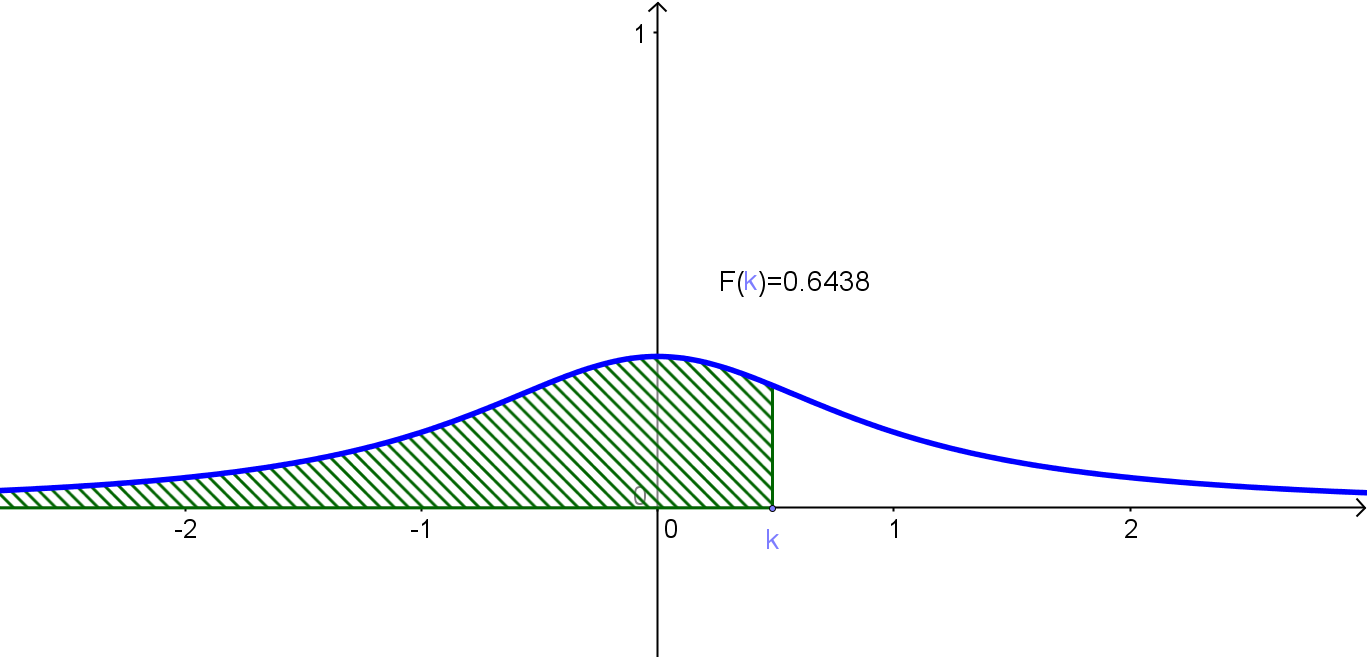
\includegraphics[width=12cm]{../fig/Cap05-DistribucionCauchy-ColaIzquierda.png}
\end{enColor}
\begin{bn}
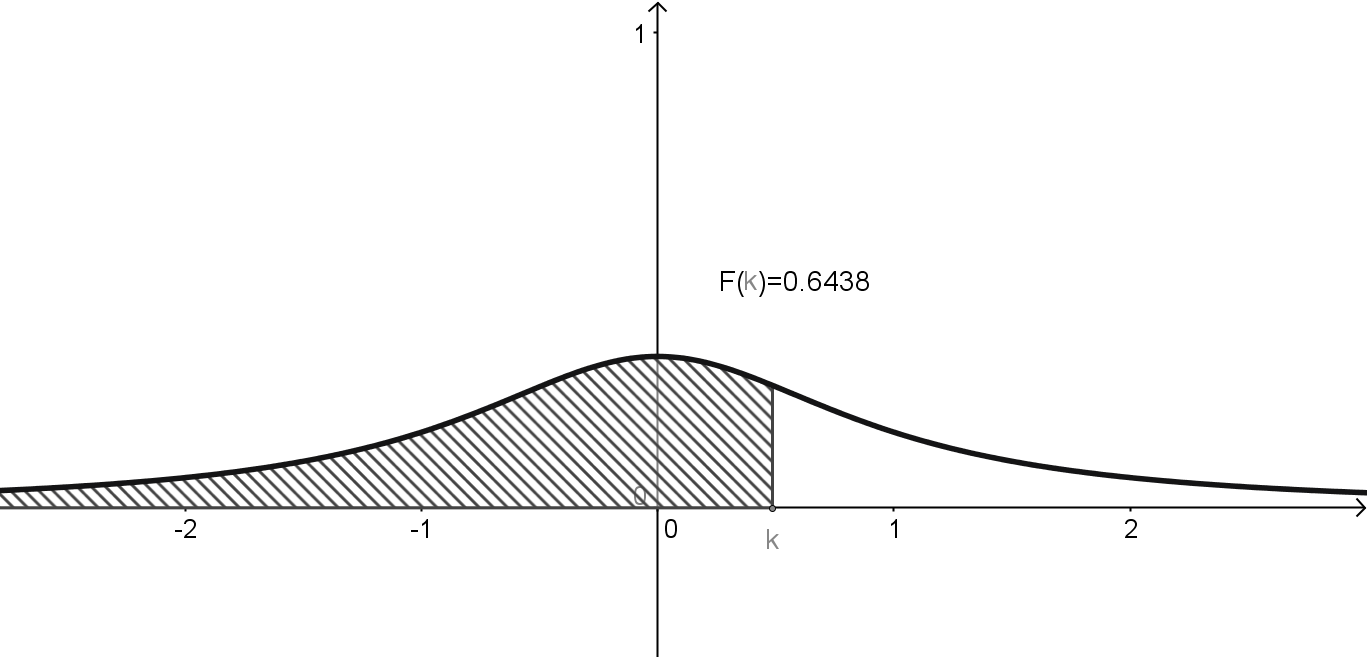
\includegraphics[width=12cm]{../fig/Cap05-DistribucionCauchy-ColaIzquierda-bn.png}
\end{bn}
\caption{Cola izquierda de la distribución de $X$ para el valor $k\approx 0.486$. El área sombreada es $F(k)=P(X\leq k)$}
\label{cap05:fig:ColaIzquierdaDistribucion}
\end{center}
\end{figure}


\begin{figure}[htb]
\begin{center}
\begin{enColor}
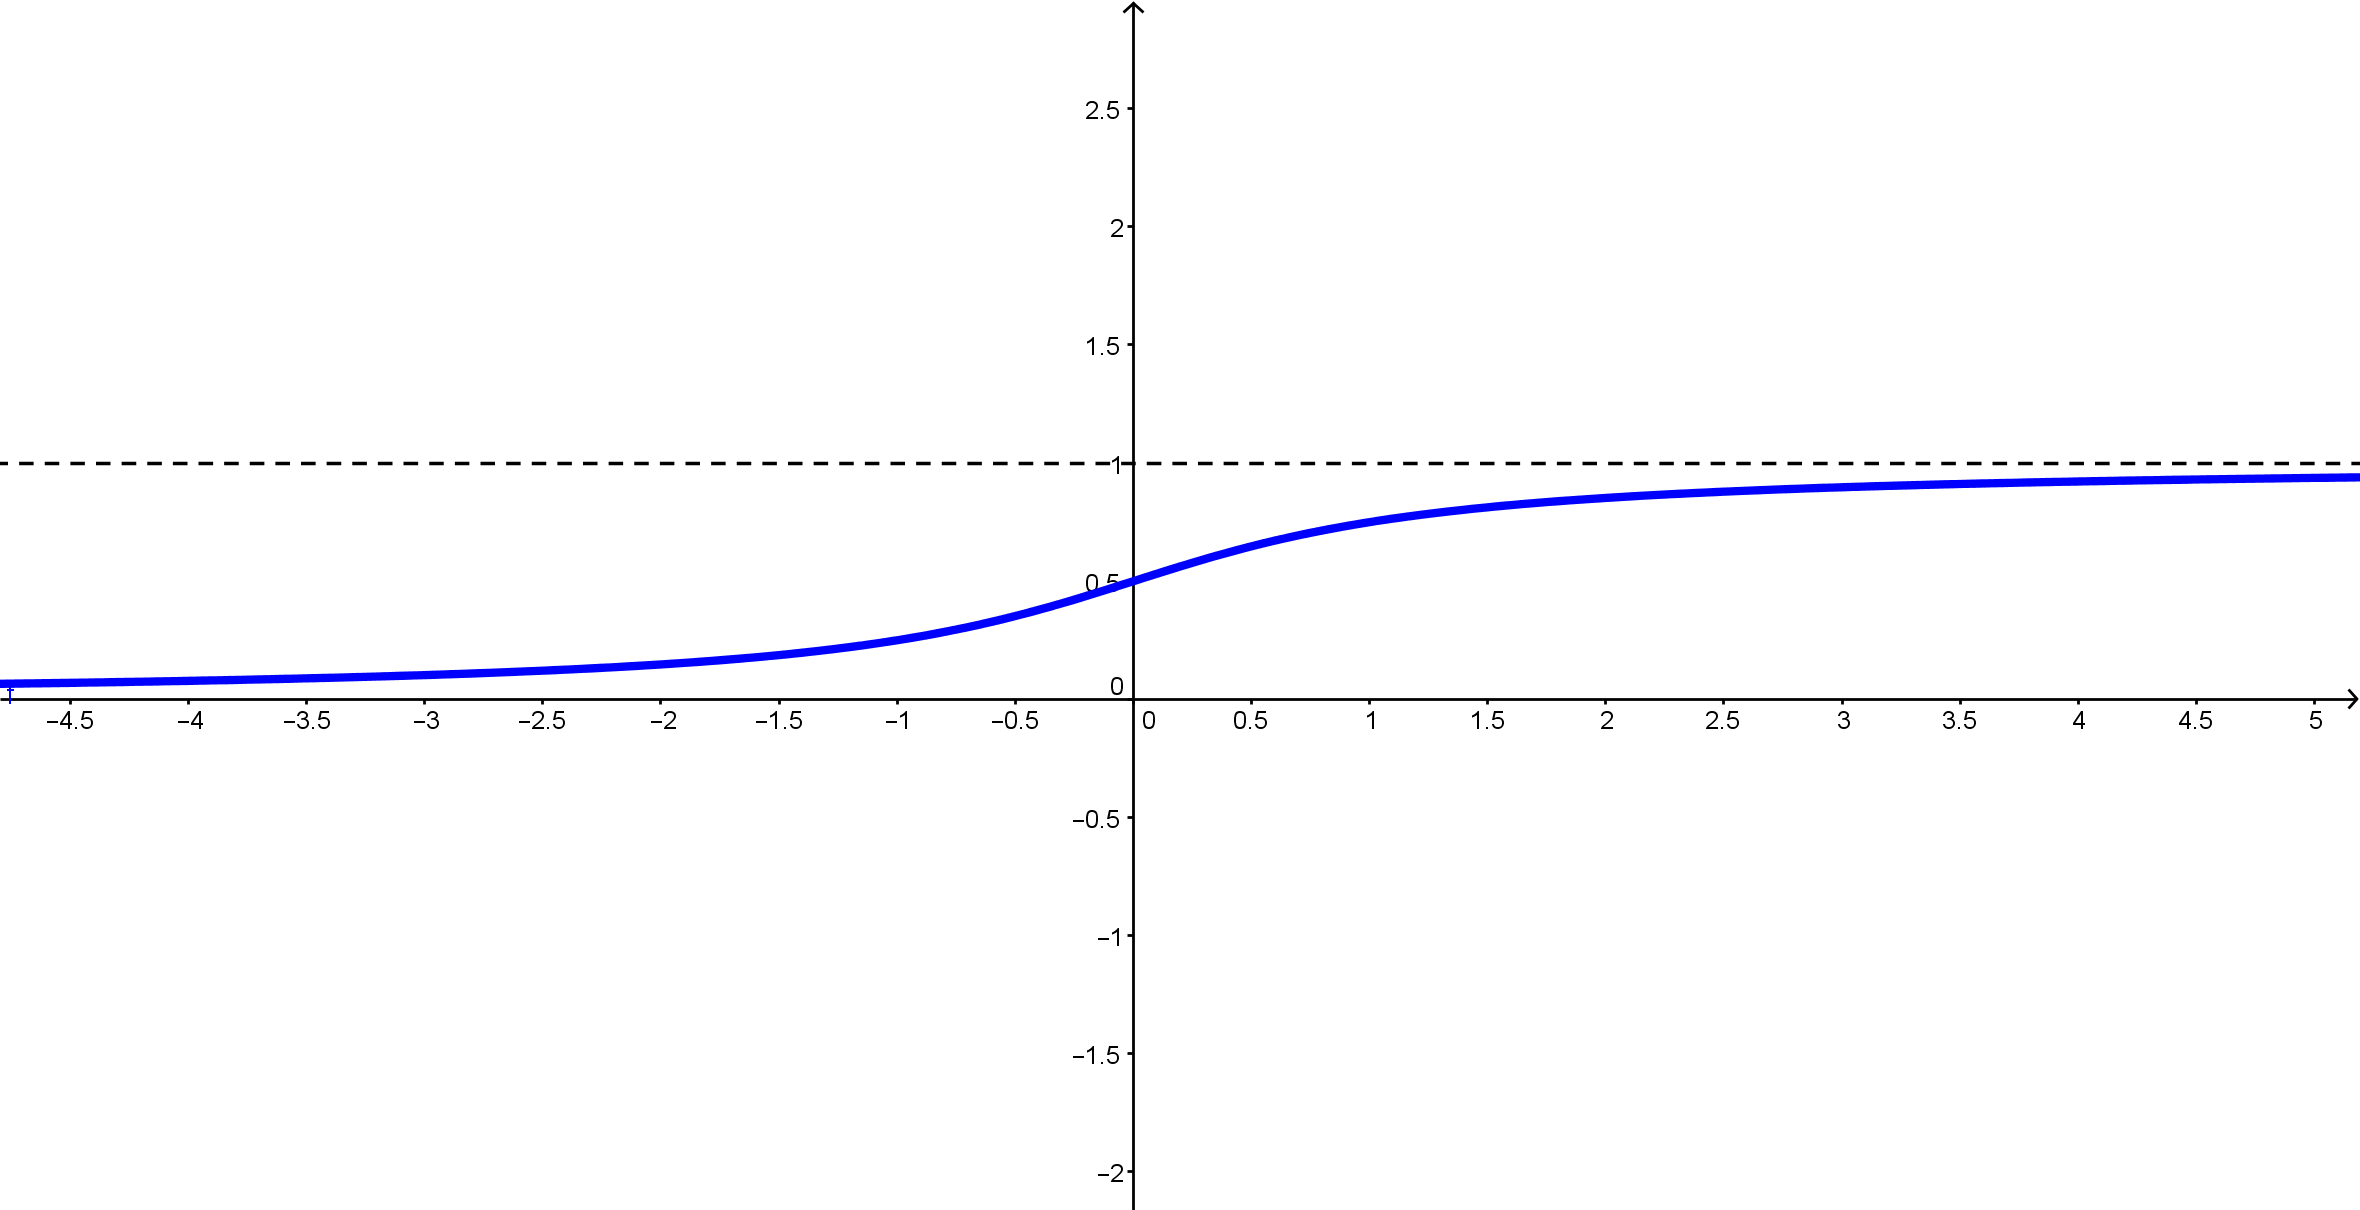
\includegraphics[width=12cm]{../fig/Cap05-FuncionDistribucionVariableCauchy.png}
\end{enColor}
\begin{bn}
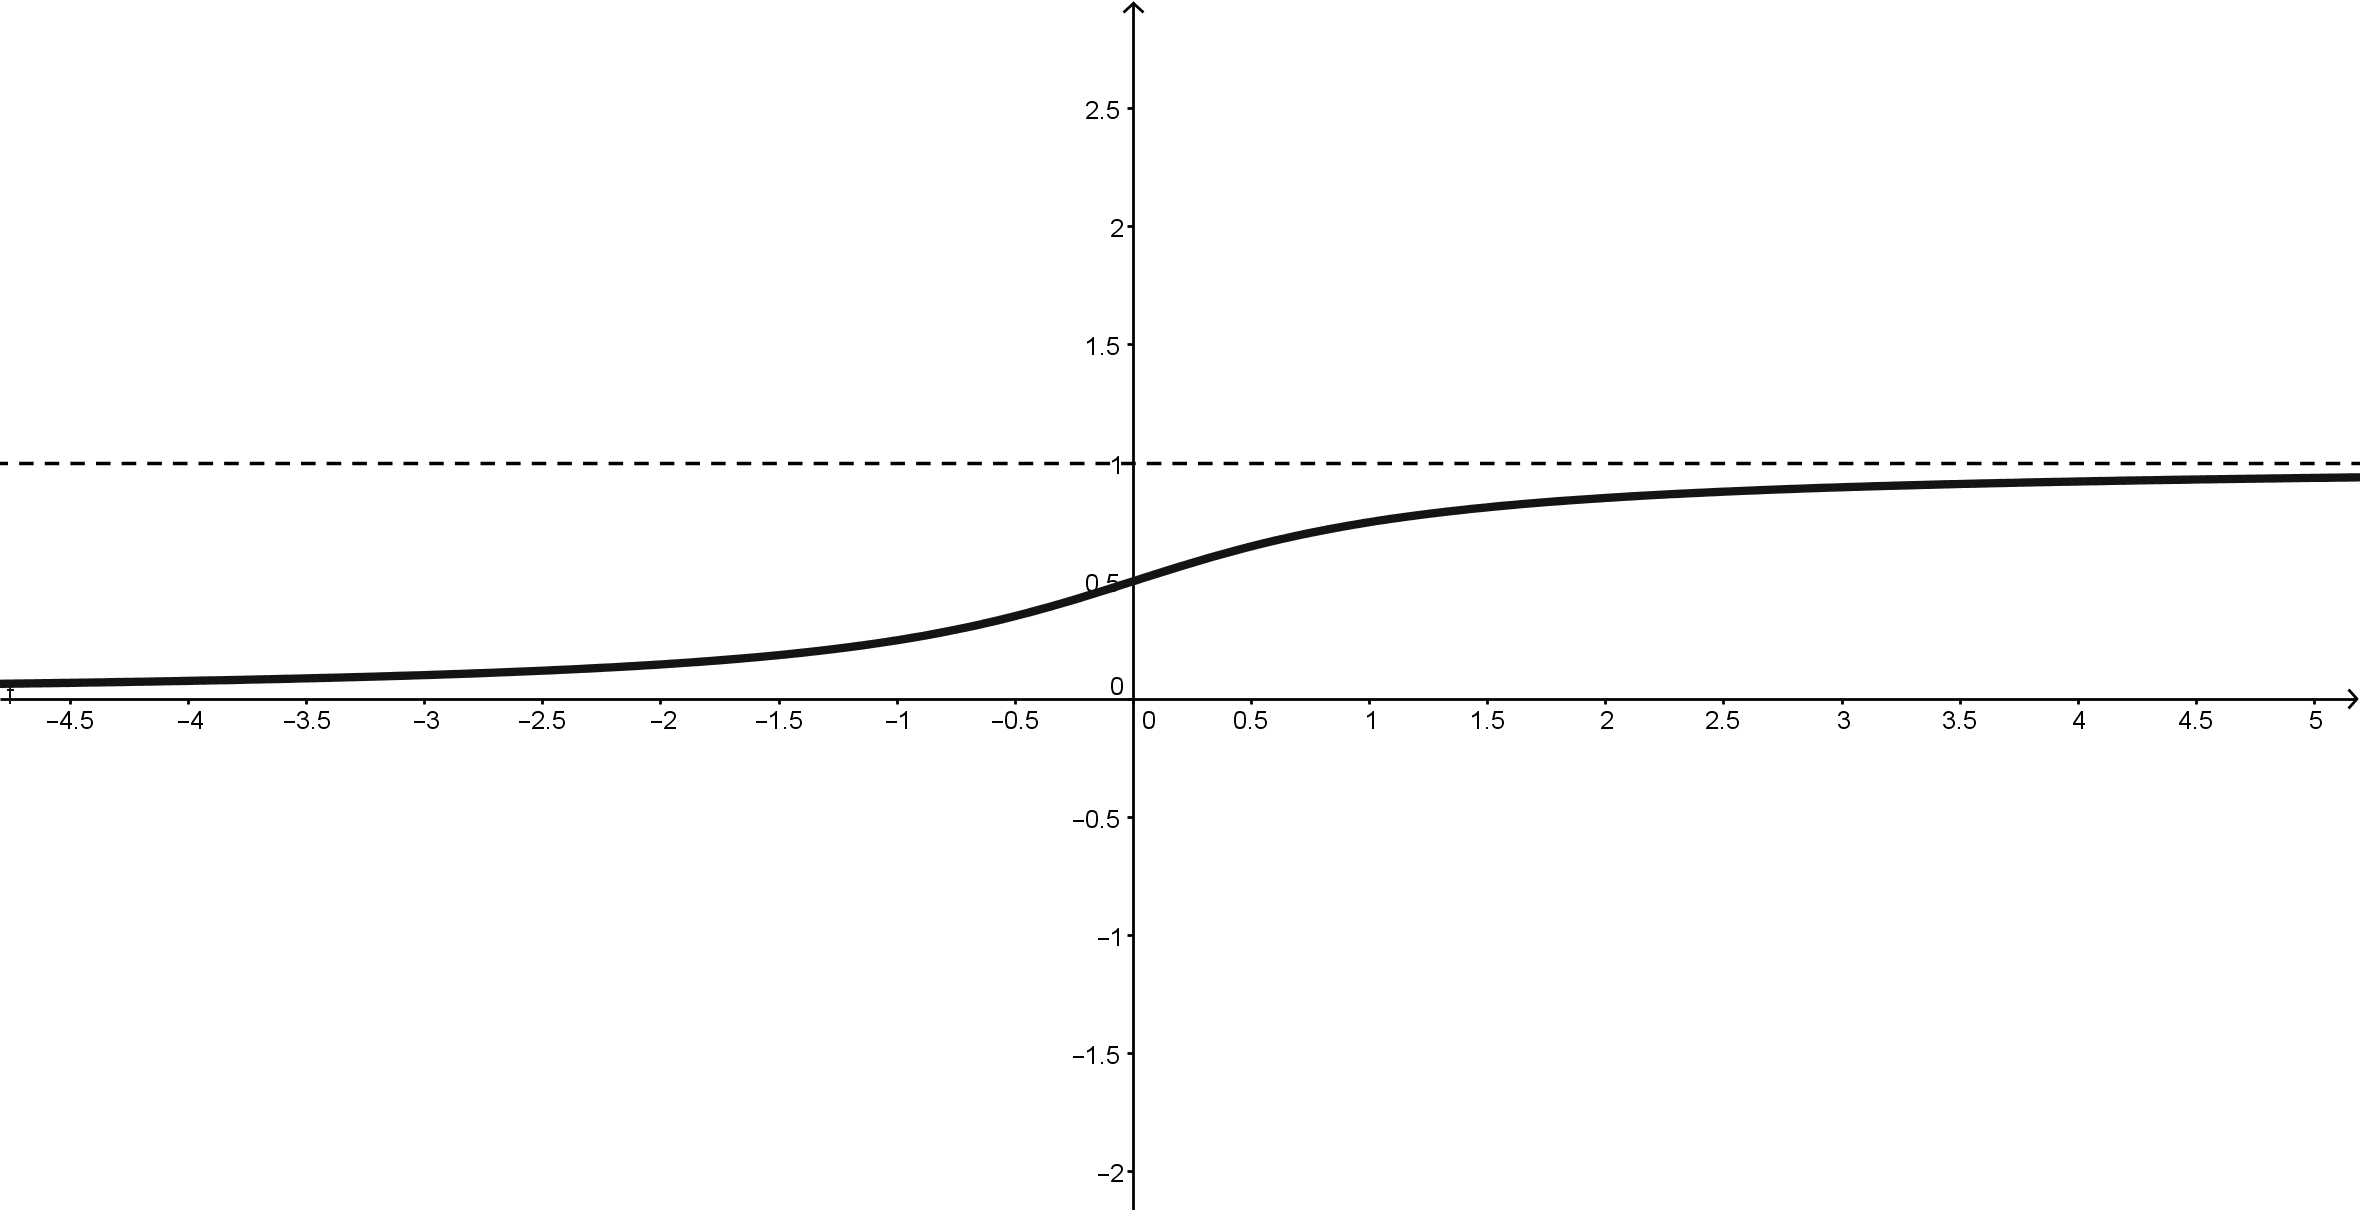
\includegraphics[width=12cm]{../fig/Cap05-FuncionDistribucionVariableCauchy-bn.png}
\end{bn}
\caption{Función de distribución $F(k)$ del ejemplo \ref{cap05:ejem:FuncionDistribucionVariableContinua}}
\label{cap05:fig:FuncionDistribucionCauchy}
\end{center}
\end{figure}

\qed
\end{ejemplo}

Como hemos dicho, la función de distribución, calculada en el punto $k$, representa la probabilidad de la  cola izquierda definida por $k$ en la distribución de probabilidad de la variable $X$. La {\sf cola izquierda}\index{cola izquierda de una distribución continua} es la región que, para la función de densidad del Ejemplo \ref{cap05:ejem:FuncionDistribucionVariableContinua}, se representa en la Figura \ref{cap05:fig:ColaIzquierdaDistribucion}. También, naturalmente, puede definirse una cola derecha (con $\geq$). Pero la función de distribución siempre se define usando la cola izquierda (con $\leq$).

Enseguida vamos a volver sobre esto, pero queremos destacar algunas características de la gráfica de la función de distribución de este ejemplo, y que tienen que ver con el hecho de que la función de distribución mide la {\em probabilidad acumulada} en la cola izquierda de $k$. Como puede verse, hacia la parte izquierda de la gráfica (hacia $-\infty$), la función de distribución vale prácticamente $0$. Después, a medida que avanzamos, y la probabilidad se va acumulando, la función $F$ va creciendo (nunca puede bajar), hasta que, en la parte derecha de la gráfica (hacia $+\infty$), el valor de $F$ es prácticamente $1$.  Estas características, con los matices que exploraremos en el próximo apartado, son comunes a las funciones de distribución de todas las variables aleatorias continuas.

La función de distribución sirve, entre otras cosas, para calcular con facilidad la probabilidad de un intervalo cualquiera. Por ejemplo, si $X$ es una variable aleatoria continua $X$ cualquiera, y queremos saber la probabilidad de que $X$ tome valores en el intervalo $(a,b)$, podemos responder usando esta ecuación:
\[P(a<X<b) = F(b) - F(a)\]
Esta igualdad es fácil de entender gráficamente, como la diferencia entre la cola izquierda que
define $b$, menos la cola izquierda que define $a$. En próximos capítulos y tutoriales tendremos
sobradas ocasiones de volver sobre estas ideas, así que aquí no nos vamos a extender mucho más.
%Sï queremos adelantar algo relacionado con el uso de R, para que el lector se vaya familiarizando con la terminología. En R, las funciones de distribución se reconocen porque sus nombre empiezan con la letra {\tt p}. Por ejemplo, la función de distribución de una variable normal se llama, en R, {\tt pnorm}. La de una variable uniforme, se llama {\tt punif}, etc.

\subsection{Cuantiles para una una variable aleatoria continua.}
\label{cap05:subsec:CuantilesVariableContinua}

Este apartado pretende ser la traducción, al caso continuo, de la discusión que hicimos en el caso discreto, dentro del apartado \ref{cap04:subsec:CuantilesVariableAleatoriaDiscreta} (pág. \pageref{cap04:subsec:CuantilesVariableAleatoriaDiscreta}). Para empezar, vamos a pensar en cuál sería el equivalente de la Figura \ref{cap04:fig:GraficaFuncionDistribucionVariableAleatoriaDiscreta} (pág. \pageref{cap04:fig:GraficaFuncionDistribucionVariableAleatoriaDiscreta}). Es decir, ¿cuál es el aspecto típico de la función de distribución de una variable aleatoria continua? En general, podemos asumir que la función de densidad $f(x)$ será, al menos, {\em continua a trozos} (eso significa que su gráfica puede incluir algunos ``saltos'', pero no comportamientos más raros). Y, si es así, puesto que $F(k)$ se obtiene integrando $f(x)$, y el proceso de integración siempre hace que las funciones sean más ``regulares'', con gráficas más suaves,  el resultado será una función de distribución $F$ que es continua, y (no estrictamente) creciente, cuyo valor es esencialmente $0$ hacia la izquierda de la gráfica (hacia $-\infty$) y esencialmente $1$ hacia la derecha de la gráfica (hacia $+\infty$).

\begin{figure}[h!]
\begin{center}
\begin{enColor}
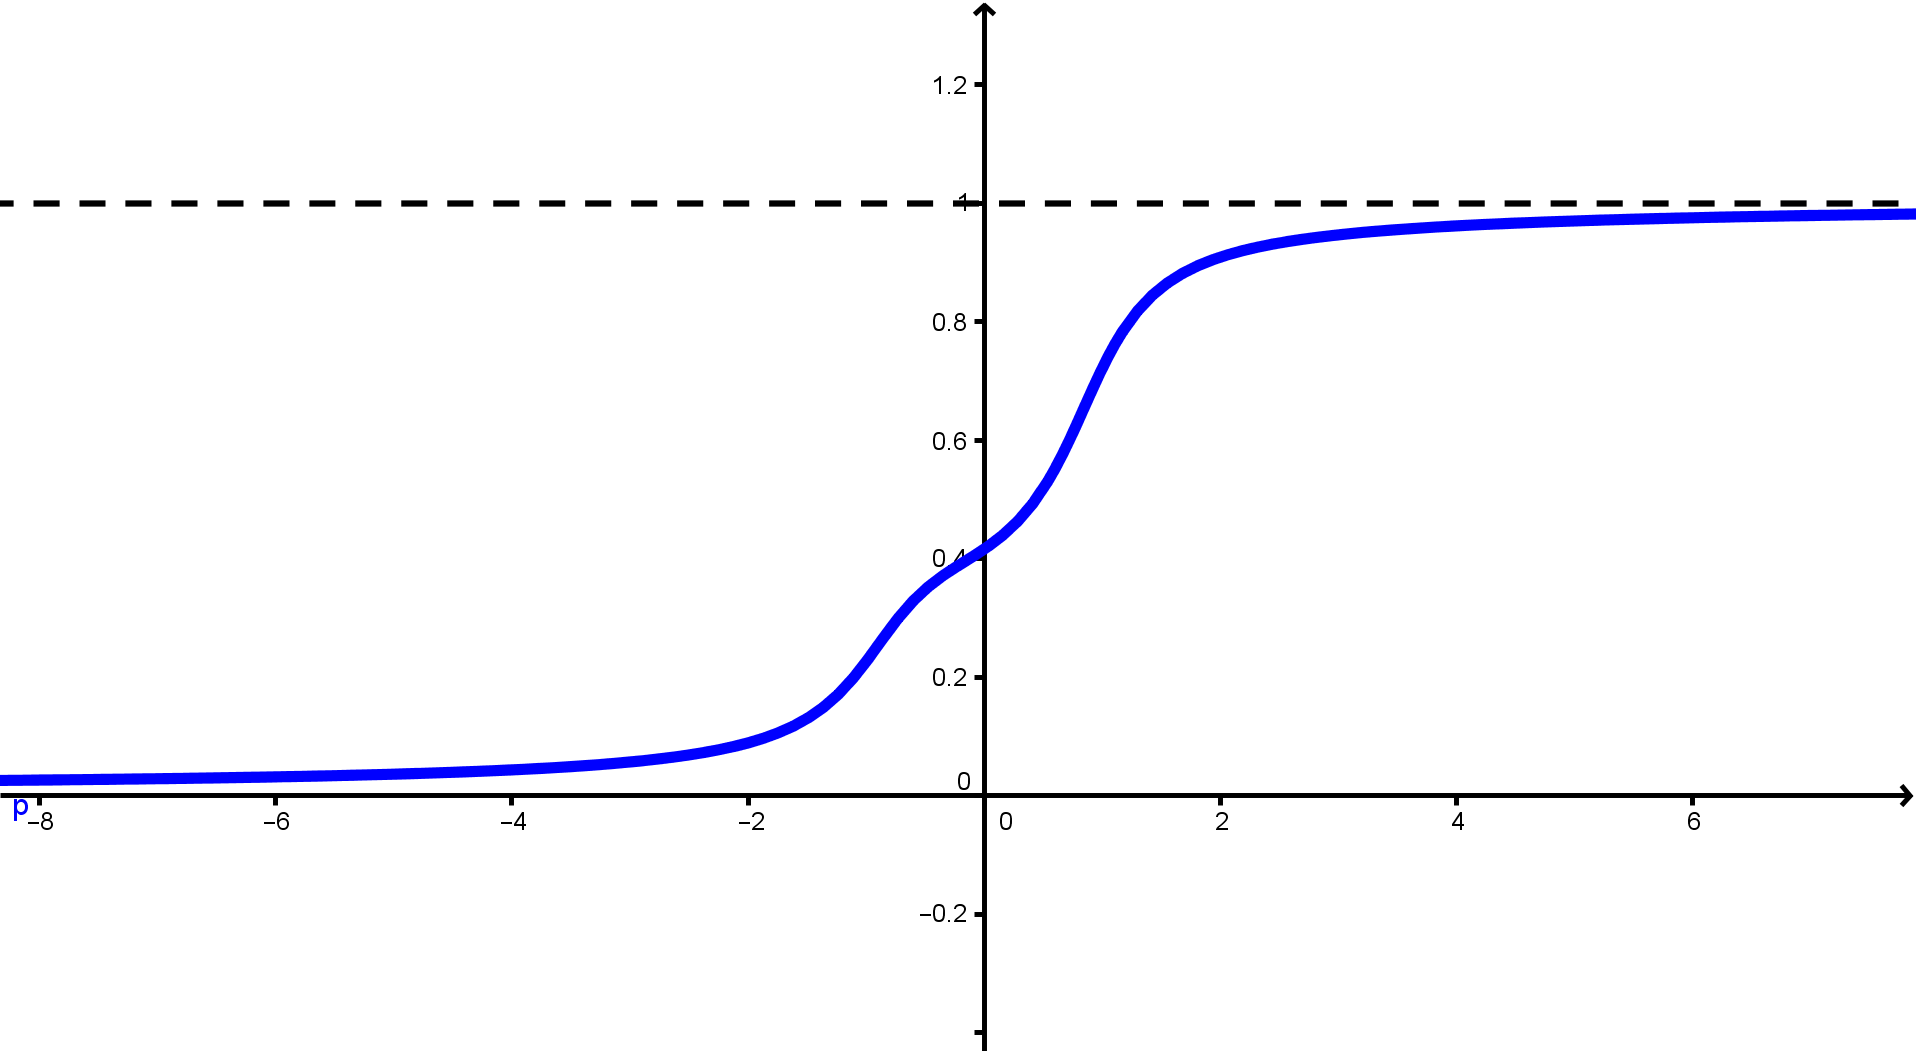
\includegraphics[width=7.5cm]{../fig/Cap05-FuncionDistribucionVariableContinuaTipica.png}
\end{enColor}
\begin{bn}
\includegraphics[width=7.5cm]{../fig/Cap05-FuncionDistribucionVariableContinuaTipica-bn.png}
\end{bn}
\caption{Una ``típica'' función de distribución de una variable aleatoria continua.}
\label{cap05:fig:TipicaFuncionDistribucionVariableContinua}
\end{center}
\end{figure}
\noindent Hemos tratado de representar las características de lo que sería una típica función de
distribución en la Figura \ref{cap05:fig:TipicaFuncionDistribucionVariableContinua}. Como puede
verse en esa figura, la función $F$ sube desde el $0$ hasta el $1$, serpenteando (con un cambio de
concavidad por cada máximo o mínimo local de $f$). Puede estabilizarse y permanecer horizontal en
algún intervalo (ahora veremos un ejemplo), pero lo que no hace nunca es bajar (es {\em no
decreciente}), ni dar saltos (es {\em continua}).

En el caso de las funciones de densidad con soporte en un intervalo (o intervalos), estas características no se modifican, pero se adaptan a los intervalos en los que $f$ es distinta de cero. Vamos a ver un ejemplo para ilustrar esta cuestión.
\begin{ejemplo}
\label{cap05:ejem:FuncionDistribucionDensidadSoporteIntervalos}
Vamos a considerar la función de densidad definida así:
\[f(x)=
\begin{cases}
\dfrac{2x}{3}&\mbox{, cuando }0\leq x\leq 1\\[3mm]
\dfrac{4}{3}\cdot(3-x)&\mbox{, cuando }2\leq x\leq 3\\[3mm]
0&\mbox{, en cualquier otro caso.}
\end{cases}\]
cuya gráfica puede verse en la Figura \ref{cap05:fig:EjemploFuncionDistribucionDensidadSoporteIntervalos}.

\begin{figure}[bh!]
\begin{center}
\begin{enColor}
\includegraphics[width=10cm]{../fig/Cap05-EjemploFuncionDistribucionDensidadSoporteIntervalos.png}
\end{enColor}
\begin{bn}
\includegraphics[width=10cm]{../fig/Cap05-EjemploFuncionDistribucionDensidadSoporteIntervalos-bn.png}
\end{bn}
\caption{Gráfica de la función de densidad del Ejemplo \ref{cap05:ejem:FuncionDistribucionDensidadSoporteIntervalos}.}
\label{cap05:fig:EjemploFuncionDistribucionDensidadSoporteIntervalos}
\end{center}
\end{figure}
\noindent Vamos a calcular la función de distribución $F(k)$, explicando paso a paso el cálculo, que depende de la región donde tomemos el valor $k$. Obviamente, si $k<0$, entonces (puesto que $f$ es $0$ a la izquierda del origen), se tiene:
\[F(k)=P(X\leq k)=0.\]
A continuación, si $0\leq k\leq 1$, usamos en la integral la definición de $f(x)$ en el intervalo $(0,1)$, y tenemos:
\[F(k)=P(X\leq k)=\int_0^k \dfrac{2x}{3}dx=\dfrac{k^2}{3}.\]
Puedes comprobar esta integral con cualquiera de las herramientas que se explican en el Tutorial05. Ahora, si $1<k<2$, se tiene:
\[F(k)=P(X\leq k)=P(X\leq 1)=F(1)=\dfrac{1}{3}.\]
Este es el resultado que puede parecer más chocante, y una de las razones principales por las que incluimos este ejemplo. Para entenderlo, hay que pensar que, mientras $k$ avanza a lo largo del intervalo $(1,2)$, puesto que $f$ es $0$ en ese intervalo, no hay probabilidad ``nueva'' que  acumular. La probabilidad acumulada, en ese intervalo, es la que ya habíamos acumulado hasta $k=1$ (el área del primer ``triángulo'' que define $f$). Es decir, que $F$ se mantiene constante, e igual a $F(1)$, en todo el intervalo $(1,2)$. Esta es la situación a la que nos referíamos en los párrafos previos al ejemplo, cuando decíamos que la función de distribución puede ``estabilizarse y quedar horizontal'' en un intervalo.

Una vez que $k$ entra en el intervalo $(2,3)$, la probabilidad vuelve a aumentar. Y tenemos:
\[F(k)=\int_0^k f(x)dx=\int_0^1 f(x)dx + \int_1^2 f(x)dx+ \int_2^k f(x)dx.\]
Esta identidad, que puede intimidar al principio, simplemente dice que dividimos la integral (el área bajo la gráfica de $f$), que va desde $0$ hasta $k$,  en tres tramos (tres integrales, o tres áreas), definidos por los intervalos $(0,1)$, $(1,2)$ y $(2,k)$, respectivamente. La primera de las tres integrales es simplemente el área del triángulo de la izquierda, que coincide con $F(1)=\frac{1}{6}$. La segunda integral vale $0$, porque $f$ es $0$ en el intervalo $(1,2)$. Así que:
\[F(k)=\int_0^k f(x)dx=\frac{1}{3} + 0 + \int_2^k f(x)dx.\]
Y para calcular esta última integral basta sustituir la definición de $f$ en $(2,3)$:
\[F(k)=\int_0^k f(x)dx=\frac{1}{3} + 0 + \int_2^k \dfrac{4}{3}\cdot(3-x)dx=
\frac{1}{3} +0-\frac{2}{3}\cdot(k^2-6 k+8).\]
Hemos mantenido el $1/3$ y el $0$ para que al lector le resulte más fácil identificar de donde proviene cada término de la suma. Simplificando, para $2\leq k\leq 3$ se tiene:
\[F(k)=-\dfrac{2 k^2}{3}+4 k-5.\]
En particular, puedes comprobar que $F(3)=1$. Esto refleja el hecho de que, cuando $k$ llega a $3$,
y hemos acumulado toda la probabilidad posible, y por eso $F$ alcanza el valor $1$. A partir de ese
momento, sea cual sea el valor $k>3$ que se considere, siempre será $F(k)=1$, porque, insistimos,
$F$ es la probabilidad acumulada, y ya hemos acumulado toda la probabilidad disponible. Si ponemos
juntas todas las piezas, hemos obtenido:
\[F(k)=
\begin{cases}
0,&\mbox{ cuando } k<0\\[3mm]
\dfrac{k^2}{6},&\mbox{ cuando }0\leq k\leq 1\\[3mm]
\dfrac{1}{3},&\mbox{ cuando }1\leq k\leq 2\\[3mm]
-\dfrac{2 k^2}{3}+4 k-5,&\mbox{ cuando }2\leq k\leq 3\\[3mm]
1,&\mbox{ cuando }k>3.
\end{cases}\]
La gráfica de la función de distribución $F(k)$ puede verse en la Figura
\ref{cap05:fig:EjemploFuncionDistribucionDensidadSoporteIntervalos02}. En esa figura se aprecia que
$F(k)$ es, como decíamos, continua, creciente de forma no estricta (hay un tramo horizontal, pero
no hay bajadas), y vale $0$ a la izquierda, y $1$ a la derecha.

\begin{figure}[h!]
\begin{center}
\begin{enColor}
\includegraphics[width=10cm]{../fig/Cap05-EjemploFuncionDistribucionDensidadSoporteIntervalos02.png}
\end{enColor}
\begin{bn}
\includegraphics[width=10cm]{../fig/Cap05-EjemploFuncionDistribucionDensidadSoporteIntervalos02-bn.png}
\end{bn}
\caption{Gráfica de la función de distribución $F(k)$ del Ejemplo \ref{cap05:ejem:FuncionDistribucionDensidadSoporteIntervalos}.}
\label{cap05:fig:EjemploFuncionDistribucionDensidadSoporteIntervalos02}
\end{center}
\end{figure}
\qed
\end{ejemplo}
Después de familiarizarnos un poco más con las propiedades de las funciones de distribución de las variables continuas, estamos listos para la definición de {\sf cuantil} de una variable aleatoria continua.
    \begin{center}
    \fcolorbox{black}{Gris025}{
    \begin{minipage}{12cm}
        \begin{center}
        {\bf Cuantil $p_0$ de una variable aleatoria continua}
        \index{cuantil de una variable aleatoria continua}
        \end{center}
        Si $X$ es una variable aleatoria continua, cuya función de distribución es $F(x)$, entonces, dada una probabilidad $p_0$ cualquiera, el {\sf cuantil} $p_0$ de $X$ es {\bf el menor valor} $x^*$ que cumple:
        \begin{equation}
        \label{cap05:ecu:CuantilVariableAleatoriaContinua}
            F(x^*)=p_0.
        \end{equation}
    \end{minipage}}
    \end{center}
Si la comparas con la definición del caso discreto (pág. \pageref{cap04:ecu:CuantilVariableAleatoriaDiscreta}), verás que dicen esencialmente lo mismo. Es importante subrayar que, de nuevo, hemos tenido que definir el cuantil como {\em el menor valor} que  cumple la Ecuación \ref{cap05:ecu:CuantilVariableAleatoriaContinua}, porque, como muestra la zona horizontal de la gráfica en la Figura \ref{cap05:fig:EjemploFuncionDistribucionDensidadSoporteIntervalos02}, puede suceder que haya infinitos valores $x$ que cumplan esa ecuación (en ese Ejemplo \ref{cap05:ejem:FuncionDistribucionDensidadSoporteIntervalos}, todos los valores del intervalo $(1,2)$).

\begin{ejemplo}{\bf (Continuación del Ejemplo \ref{cap05:ejem:FuncionDistribucionDensidadSoporteIntervalos})}
\label{cap05:ejem:FuncionDistribucionDensidadSoporteIntervalos02}
Si fijamos $p_0=\frac{1}{2}$, ¿cuál el cuantil $p_0$ de la variable $X$ de este ejemplo? Es decir, ¿cuál es su {\em mediana}? La ecuación
\[F(k)=\dfrac{1}{2},\]
en este caso, tiene una única solución, como se ilustra en la Figura \ref{cap05:fig:EjemploFuncionDistribucionDensidadSoporteIntervalos03}.

\begin{figure}[h]
\begin{center}
\begin{enColor}
\includegraphics[width=10cm]{../fig/Cap05-EjemploFuncionDistribucionDensidadSoporteIntervalos03.png}
\end{enColor}
\begin{bn}
\includegraphics[width=10cm]{../fig/Cap05-EjemploFuncionDistribucionDensidadSoporteIntervalos03-bn.png}
\end{bn}
\caption{Buscando la mediana de la variable $X$ del Ejemplo \ref{cap05:ejem:FuncionDistribucionDensidadSoporteIntervalos}.}
\label{cap05:fig:EjemploFuncionDistribucionDensidadSoporteIntervalos03}
\end{center}
\end{figure}

En esa figura es evidente que la mediana pertenece al intervalo $(2,3)$. La mediana es, entonces, la única solución positiva de:
\[-\dfrac{2 k^2}{3}+4 k-5=\dfrac{1}{2}.\]
Y se obtiene
\[k = 3-\dfrac{\sqrt{3}}{2} \approx 2.1340\]
Cambiando ahora al valor $p_0=\frac{1}{3}$. ¿Cuál es el cuantil correspondiente? En este caso, como ya hemos discutido, todos los valores del intervalo $1\leq k\leq 2$ cumplen
\[F(k)=\dfrac{1}{3}.\]
Así que, para localizar el cuantil, debemos elegir el menor de ellos; esto es, el cuantil $1/3$ es igual a $1$.
\qed
\end{ejemplo}


\subsection{Variables mudas en las integrales.}
\label{cap05:subsec:VariablesMudasIntegrales}
\noindent{\bf Opcional: esta sección puede omitirse en una primera lectura.} Es recomendable leerla,
en cualquier caso, si tienes problemas para entender la notación del diferencial $dx$ que usamos en las integrales.\\

Hemos usado el símbolo $k$ para la variable de la función $F$, para de ese modo poder seguir empleando el símbolo $x$ dentro de la integral, y especialmente en el diferencial $dx$. Somos conscientes de que, para los  usuarios de la Estadística con menos preparación matemática, este asunto de la variable que aparece en el diferencial resulta confuso y genera una cierta inseguridad. Por esa razón mantenemos el diferencial $dx$, que resultará más familiar (si acaso) a estos lectores. Los lectores más sofisticados desde el punto de vista matemático sabrán que la variable que aparece en el diferencial es, como se suele decir, una {\sf variable muda}. ¿Qué quiere decir eso? Lo entenderemos mejor con el ejemplo de un sumatorio. Si escribimos
\[\sum_{k=1}^{10} k^2 \]
el símbolo significa {\em suma de los cuadrados de los números del 1 al 10}. Es decir,
\[\sum_{k=1}^{10} k^2 = 1^2 + 2^2 +  3^2 + 4^2 + 5^2 + 6^2 + 7^2 + 8^2 + 9^2 + 10^2 = 385 \]
¿Y si cambio $k$ por $j$? Es decir:
\[\sum_{j=1}^{10} j^2 \]
Está claro que la suma es la misma, los cuadrados de los números del 1 al 10, y el resultado es el mismo $385$ de antes. Es decir, que podemos escribir:
\[\sum_{k=1}^{10} k^2 = \sum_{j=1}^{10} j^2 = \sum_{p=1}^{10} p^2 = \sum_{h=1}^{10} h^2 =\cdots \]
y es en ese sentido en el que decimos que la variable que se usa en el sumatorio es una {\em variable muda}.

Con las integrales ocurre lo mismo, de manera que
\[\int_0^1 x^2 dx = \int_0^1 y^2 dy = \int_0^1 z^2 dz = \int_0^1 v^2 dv = \cdots \]
Todas estas integrales valen $1/2$ (puedes usar el ordenador para comprobarlo), y de nuevo, decimos
que la variable del diferencial es muda.

En la definición de la función de distribución
\[F(k)=\int_{\infty}^{k} f(x)dx.\]
tenemos que ser un poco más cuidadosos, porque intervienen dos variables, la $k$ y la $x$. Otro ejemplo con sumatorios puede ayudar a aclarar esto. El sumatorio
\[\sum_{k=1}^n k^2 \]
representa la suma de los cuadrados de los $n$ primeros números. ¿Y quién es $n$? Un número {\em
variable}, que concretaremos en cada caso concreto. El resultado de la suma, por supuesto, depende
de $n$, así que tiene sentido decir que hemos definido una función
\[S(n)=\sum_{k=1}^n k^2\]
Por ejemplo
\[S(3)=\sum_{k=1}^3 k^2 = 1^2 + 2^2+ 3^2 = 13.\]
En este ejemplo en particular hay una fórmula alternativa, sin sumatorios, para calcular los
valores de esa función:
\[S(n)=\sum_{k=1}^n k^2 = \dfrac{1}{6}n(n+1)(2n+1)\]
Esta fórmula debe servir para dejar más claro aún que $S(n)$ es, de hecho, una función de $n$.  De
la misma forma, cuando vemos el símbolo
\[F(k)=\int_{\infty}^{k} f(x)dx\]
tenemos que entender que $k$ es una variable (como la $n$ de antes), que se fijará en cada caso concreto, mientras que la $x$ es muda, y sólo nos sirve para poder escribir la integral con más claridad.

Si el lector ha entendido estas ideas, entonces debería estar claro que podemos escribir
\[F(k)=P(X\leq k)=\int_{\infty}^{k} f(x)dx\]
y también (cambiando $k$ por $u$)
\[F(u)=\int_{\infty}^{u} f(x)dx\]
y también
\[F(u)=\int_{\infty}^{u} f(s)ds\]
y esas tres expresiones definen todas ellas la misma función. De hecho podemos definir la misma función intercambiando completamente los papeles de $x$ y $k$:
\[F(x)=\int_{\infty}^{x} f(k)dk\]

\section{Distribución normal y Teorema central del límite.}
\label{cap05:sec:DistribucionNormalTCL}

Ahora que disponemos del vocabulario básico de las variables aleatorias continuas, podemos volver al descubrimiento de De Moivre, que se puede expresar más claramente en este nuevo lenguaje. Lo que De Moivre descubrió es esto:
    \begin{center}
    \fcolorbox{black}{Gris025}{
    \begin{minipage}{12.5cm}
        Para valores de $n$ grandes, la variable aleatoria discreta de tipo binomial $B(n,p)$ se puede aproximar bien usando una variable aleatoria de tipo continuo, cuya función de densidad es la que aparece en la Ecuación \ref{cap05:ecu:EcuacionCurvaNormal} de la página \pageref{cap05:ecu:EcuacionCurvaNormal}.
        %%%%%%%%%%%%%%%%%%%%%%%%%%%%%%%%%%%%%%%
    \end{minipage}}
    \end{center}
Esta relación con la binomial hace que esa variable aleatoria continua sea la más importante de todas, y es la razón por la que le vamos a dedicar una atención especial en esta sección. Vamos a empezar por ponerle  nombre, y reconocer algo que la notación ya habrá hecho sospechar al lector:
    \begin{center}
    \fcolorbox{black}{Gris025}{
    \begin{minipage}{12.5cm}
        \begin{center}
        %%%%%%%%%%%%%%%%%%%%%%%%%%%%%%%%%%%%%%%
        {\bf  Variable aleatoria normal. Media y desviación típica.}
        \end{center}
        \index{variable aleatoria normal}
        \index{media de una variable aleatoria normal}
        \index{desviación típica de una variable aleatoria normal}
       %%%%%%%%%%%%%%%%%%%%%%%%%%%%%%%%%%%%%%%
       Una variable aleatoria continua $X$ es {\sf normal de tipo $N(\mu,\sigma)$} si su función de densidad es de la forma
       \begin{equation}\label{cap05:ecu:varianzaVariableAleatoriaNormal}
       f_{\mu,\sigma}(x)=\dfrac{1}{\sigma\sqrt{2\pi}}e^{-\frac{1}{2}\left(\frac{x-\mu}{\sigma}\right)^2}.
       \end{equation}
       que ya vimos en la Ecuación \ref{cap05:ecu:EcuacionCurvaNormal} (pág. \pageref{cap05:ecu:EcuacionCurvaNormal}).\\

       De hecho, $\mu$ es la media de $X$ y $\sigma>0$ es su desviación típica.
        %%%%%%%%%%%%%%%%%%%%%%%%%%%%%%%%%%%%%%%
    \end{minipage}}
    \end{center}

{\bf ADVERTENCIA:} En otros libros se usa la notación $N(\mu,\sigma^2)$ para describir la variable normal. Asegúrate de comprobar qué notación se está usando para evitar errores de interpretación.

Antes de seguir adelante vamos a ver el aspecto que tienen las funciones de densidad de las variables normales, y como dependen de los valores de $\mu$ y $\sigma$.  La Figura \ref{cap05:fig:curvasnormales-02} muestra varias de estas curvas normales, para distintos valores de $\mu$ y $\sigma$. Todas ellas tienen forma acampanada, con la cima sobre el valor $\mu$ del eje horizontal, y con una altura que depende de $\sigma$: cuanto más pequeño es $\sigma$, más alta y esbelta es la campana. Seguramente, lo mejor que puede hacer el lector para familiarizarse con estas funciones es jugar un rato con ellas, usando el ordenador. En el Tutorial05 veremos de forma dinámica cómo influyen los valores de $\mu$ y $\sigma$ sobre la forma de las curvas normales.
\begin{figure}[htbp]
\begin{center}
\begin{enColor}
\includegraphics[width=13cm]{../fig/cap05-curvasnormales-02.png}
\end{enColor}
\begin{bn}
\includegraphics[width=13cm]{../fig/cap05-curvasnormales-02-bn.png}
\end{bn}
\caption{Curvas normales, para distintos valores de $\mu$ y $\sigma$}
\label{cap05:fig:curvasnormales-02}
\end{center}
\end{figure}

Hemos aprovechado este fichero para presentar una propiedad especialmente significativa de la familia de variables aleatorias normales, que el lector hará bien en memorizar, porque estos valores son muy útiles.    %\[P(\mu-\sigma<X<\mu+\sigma)\approx 0.68\mbox{, y también }P(\mu-2\sigma<X<\mu+2\sigma)\approx 0.95.\]
    \begin{center}
    \fcolorbox{black}{Gris025}{
    \begin{minipage}{12.5cm}
        \begin{center}
        %%%%%%%%%%%%%%%%%%%%%%%%%%%%%%%%%%%%%%%
        {\bf  Regla 68-95-99 para distribuciones normales.}
        \index{regla 68-95-99, distribuciones normales}
        \index{68-95-99, regla para distribuciones normales}
        \end{center}
       %%%%%%%%%%%%%%%%%%%%%%%%%%%%%%%%%%%%%%%
       Si $X$ es una variable normal de tipo $N(\mu,\sigma)$ entonces se cumplen estas aproximaciones (las probabilidades con tres cifras significativas):
            \begin{equation}
            \label{cap05:ecu:Regla68-95-99Normales}
            \begin{cases}
            P(\mu-\sigma<X<\mu+\sigma)\approx 0.683,\\[3mm]
            P(\mu-2\sigma<X<\mu+2\sigma)\approx 0.955\\[3mm]
            P(\mu-3\sigma<X<\mu+3\sigma)\approx 0.997
            \end{cases}
            \end{equation}
    \end{minipage}}
    \end{center}
Ya sabemos que usamos la media como representante de un conjunto de datos, y que la desviación típica mide cómo de agrupados están los datos, con respecto a la media. Lo que dicen estas dos desigualdades es que, si tenemos datos de tipo normal (lo cual, como veremos, sucede a menudo), el 68\% de los datos no se aleja de la media más de $\sigma$, y hasta un 95\% de los datos está a distancia menor que $2\sigma$ de la media. Cuando estamos mirando datos de tipo normal, podemos medir la distancia de un dato a la media usando como unidad la desviación típica $\sigma$. Un dato que esté a $\sigma$ o menos de distancia es un valor bastante típico de esa variable, mientras que si un dato está a distancia mayor que $6\sigma$ de la media, podemos decir que es un valor extremadamente raro (y es muy improbable que la variable tome ese valor).

Estas variables aleatorias normales son, insistimos, excepcionalmente importantes. En primer lugar, porque tienen esa relación especial con las binomiales, y las binomiales, a su vez, son las más importantes de las variables aleatorias discretas. Vamos a recapitular los detalles de esa relación de aproximación, porque hay un detalle importante que el lector debe conocer, pero que hasta ahora hemos omitido, para no interrumpir la discusión.

En la Sección \ref{sec:distribucionesContinuasEntranEscena} (ver concretamente la discusión que empieza en la pág. \pageref{cap05:lugar:DiscusionAproximarBinomialNormal}) hemos planteado el problema de calcular la probabilidad $P(300\leq X\leq 600)$ para la distribución binomial $B(1000,1/3)$. Y dijimos entonces que lo hacíamos calculando la  integral:
\[\int_{300}^{600}f_{1000,1/3}(x)dx,\]
donde $f_{1000,1/3}(x)$ era una curva normal, con $f$ como en la Ecuación \ref{cap05:ecu:varianzaVariableAleatoriaNormal}. Por otra parte, en la Sección \ref{cap05:sec:MasDetallesSobreDistribucionesContinuas}, cuando vimos el Teorema Fundamental del Cálculo (pág. \pageref{cap05:ecu:TeoremaFundamentalCalculo}), presentamos una procedimiento en dos pasos para calcular una integral que empezaba con la búsqueda de una primitiva (o antiderivada). Teniendo esto en cuenta, al tratar de calcular
\begin{equation}
\label{cap05:ecu:IntegralNormalIntervalo}
\int_{300}^{600}f_{1000,1/3}(x)dx,
\end{equation}
podríamos pensar que el primer paso es encontrar una primitiva $F(x)$ de la función $f_{1000,1/3}(x)$, y después calcularíamos
\[F(600)-F(300).\]
Pero ahí, precisamente, está la dificultad que hasta ahora hemos ocultado al lector: no podremos encontrar esa primitiva. Para ser precisos, la primitiva existe, pero no tiene una fórmula sencilla, que se pueda utilizar para hacer este cálculo sin complicaciones. Hay fórmulas, desde luego, pero todas ellas dicen cosas como ``hacer esto infinitas veces''. Los matemáticos resumen esto diciendo que la función de densidad de una normal {\sf no tiene una primitiva elemental.} Insistimos: eso no significa que no haya primitiva. Lo que dice es que la primitiva es demasiado complicada para usarla, a efectos prácticos, en el cálculo del valor de la integral.

``{!`}Pues menuda broma!'', estará pensando el lector. Nos hemos embarcado en todo este asunto de la normal, y las variables aleatorias continuas, para poder aproximar la binomial mediante integrales, y ahora resulta que esas integrales no se pueden calcular...

{!`}No tan rápido! Hemos presentado el Teorema Fundamental del Cálculo como {\em una forma} de calcular integrales. Pero no hemos dicho, desde luego, que sea {\em la única forma} de calcular integrales. De hecho, los matemáticos han desarrollado, desde la época de Newton, muchos métodos para calcular el valor {\em aproximado} de una integral, sin necesidad de conocer una primitiva. Son los métodos de {\em integración numérica}. En el caso de la normal, y especialmente con la  ayuda de un ordenador, esos métodos numéricos son muy eficientes, y nos van a permitir calcular muy fácilmente integrales como la de la Ecuación \ref{cap05:ecu:IntegralNormalIntervalo}. Aprenderemos a hacerlo en el Tutorial05.


\subsection{Distribución normal estándar. Tipificación.}
\label{cap05:subsec:DistribucionNormalEstandarTipificacion}

Hemos visto que para cada combinación de valores $\mu$ y $\sigma$ hay una variable normal de tipo
$N(\mu,\sigma)$, y sabemos que cada una de ellas tiene una función de densidad en forma de curva
acampanada, como las de la Figura \ref{cap05:fig:curvasnormales-02}. Pero las relaciones entre las
distintas curvas normales son más profundas que una simple cuestión de aspecto. Para explicar esa
relación necesitamos fijarnos en la que es, a la vez, la más simple y la más importante de todas
las curvas normales:

    \begin{center}
    \fcolorbox{black}{Gris025}{
    \begin{minipage}{12.5cm}
        \begin{center}
        %%%%%%%%%%%%%%%%%%%%%%%%%%%%%%%%%%%%%%%
        {\bf  Variable normal estándar $Z$.}
        \end{center}
        \index{variable aleatoria normal estándar $Z$}
        \index{variable $Z$}
        \index{normal estándar $Z$}
       %%%%%%%%%%%%%%%%%%%%%%%%%%%%%%%%%%%%%%%
       Una variable aleatoria normal de tipo $N(0,1)$ es una {\sf normal estándar}. Por lo tanto su media es $\mu=0$ y su desviación típica es $\sigma=1$. La letra $Z$ mayúscula se usa siempre en Estadística para representar una variable normal
       estándar.

       La función de densidad de la variable normal estándar es, por tanto:
       \begin{equation}
       \label{cap05:ecu:FuncionDensidadZ}
        f_{0,1}(x)=\displaystyle\dfrac{1}{\sqrt{2\pi}}e^{-\frac{x^2}{2}}
       \end{equation}
        %%%%%%%%%%%%%%%%%%%%%%%%%%%%%%%%%%%%%%%
    \end{minipage}}
    \end{center}

En consecuencia, la letra $Z$ no debe usarse en Estadística para ningún otro fin, porque podría inducir a confusiones y errores. ¿Por qué es tan importante la normal estándar $Z$? \,Pues porque examinando la Ecuación \ref{cap05:ecu:EcuacionCurvaNormal}, que define a todas las normales, puede descubrirse que todas esas curvas se obtienen, mediante una transformación muy sencilla, a partir de $Z$.
    \begin{center}
    \fcolorbox{black}{Gris025}{
    \begin{minipage}{12.5cm}
        \begin{center}
        %%%%%%%%%%%%%%%%%%%%%%%%%%%%%%%%%%%%%%%
        {\bf  Tipificación.}
        \end{center}
       %%%%%%%%%%%%%%%%%%%%%%%%%%%%%%%%%%%%%%%
        Si $X$ es una variable aleatoria normal de tipo $N(\mu,\sigma)$, entonces la variable que se obtiene mediante la transformación
            \begin{equation}\label{cap05:ecu:Tipificacion}
               Z=\dfrac{X-\mu}{\sigma}
            \end{equation}
           es una variable normal estándar $N(0,1)$ (y por eso la hemos llamado $Z$).               A este proceso de obtener los valores de $Z$ a partir de los de $X$ se le llama {\sf tipificación}\index{tipificación}.
    \end{minipage}}
    \end{center}
Para las funciones de densidad se cumple que:
    \begin{equation}\label{cap05:ecu:RelacionFuncionesDensidadNormales}
    f_{\mu,\sigma}(x)=\dfrac{1}{\sigma}f_{0,1}\left(\dfrac{x-\mu}{\sigma}\right).
    \end{equation}
Dejamos para el lector la tarea de comprobar la Ecuación \ref{cap05:ecu:RelacionFuncionesDensidadNormales}. Debería ser una tarea fácil a partir de las ecuaciones \ref{cap05:ecu:varianzaVariableAleatoriaNormal} (pág. \pageref{cap05:ecu:varianzaVariableAleatoriaNormal}) y \ref{cap05:ecu:FuncionDensidadZ} (pág. \pageref{cap05:ecu:FuncionDensidadZ}). De esta relación de todas las normales con $Z$ se deduce, entre otras cosas, la propiedad que hemos comentado antes sobre el hecho de que el resultado
    \[P(\mu-\sigma<X<\mu+\sigma)\approx 0.68\]
no depende de $\mu$ ni de $\sigma$ (la demostración rigurosa no es trivial, porque hay que hacer un cambio de variable en una integral). Generalizando esta idea, este proceso de tipificación de las variables normales implica, entre otras cosas, que sólo necesitamos aprender a responder preguntas sobre probabilidad formuladas para el caso estándar $N(0,1)$. Todos los demás casos se reducen a este mediante la tipificación. Veamos un ejemplo.
   \begin{ejemplo}
   \label{cap05:ejem:CalculoProbabilidadPorTipificacion}
   Una variable aleatoria continua $X$ es normal, de tipo $N(400,15)$. ¿Cuál es el valor de la probabilidad $P(380\leq X\leq 420)$?\\
   Consideremos la variable aleatoria
   \[Z=\dfrac{X-\mu}{\sigma}=\dfrac{X-400}{15}.\]
   Como sabemos, $Z$ es de tipo normal estándar $N(0,1)$. Y entonces:
   \[380\leq X\leq 420\]
   significa
   \[380-400\leq X-400\leq 420-400,\mbox{ es decir }-20\leq X\leq 20,\]
   y por tanto
   \[\dfrac{-20}{15}\leq \dfrac{X-400}{15}\leq\dfrac{20}{15},\mbox{ es decir }\dfrac{-4}{3}\leq Z\leq\dfrac{4}{3},\]
   por la construcción de $Z$. En resumen:
   \[P(380\leq X\leq 420)=P\left(\dfrac{-4}{3}\leq Z\leq\dfrac{4}{3}\right)\approx P(-1.33\leq Z\leq 1.33),\]
   y como se ve lo que necesitamos es saber responder preguntas para $Z$, que es de tipo $N(0,1)$. En este caso, usando el ordenador,  obtenemos que esa probabilidad es $\approx 0.82$.\qed
   \end{ejemplo}
Este ejemplo ayuda a entender porque los valores de $N(0,1)$ son especialmente importantes. Durante mucho tiempo, hasta la generalización de los ordenadores personales, esos valores se calculaban aproximadamente, con unas cuantas cifras decimales (usando métodos numéricos), y se tabulaban. Si miras al final de la mayoría de los libros de Estadística ({!`}pero no de este!), aún encontraras esas tablas, casi como un tributo al enorme trabajo que representan, un trabajo que desde la actualidad parece casi artesano. Nosotros no necesitaremos tablas, porque el ordenador puede calcular cualquiera de esos valores para nosotros, al instante, con más precisión de la que tenían las mejores de aquellas tablas, como veremos en el Tutorial05.

\subsubsection{Suma de variables aleatorias normales}
\label{cap05:subsubsec:SumaVariablesAleatoriasNormales}

Si tenemos dos variables normales independientes, de tipos distintos, por ejemplo:
\[X_1\sim N(\mu_1,\sigma_1)\qquad \mbox{ y }\qquad X_2\sim N(\mu_2,\sigma_2),\]
entonces, ya sabemos, por lo que vimos en la Sección \ref{sec:OperacionesVariablesAleatorias} (pág. \pageref{sec:OperacionesVariablesAleatorias}) que su suma es una variable aleatoria con media
\[\mu_1+\mu_2,\]
y desviación típica
\[\sqrt{\sigma_1^2+\sigma_2^2}.\]
(Recordemos que para esto último es esencial la independencia). Esto se cumple simplemente porque se trata de variables aleatorias, sean o no normales. Pero, en el caso particular de las variables normales, las cosas son aún mejores.
    \begin{center}
    \fcolorbox{black}{Gris025}{
    \begin{minipage}{12cm}
        \begin{center}
        \bf Suma de variables normales independientes
        \index{suma de variables normales independientes}
        \index{variables normales independientes, suma}
        \index{normales independientes, suma de variables}
        \end{center}
       Si
       \[X_1\sim N(\mu_1,\sigma_1)\qquad \mbox{ y }X_2\sim N(\mu_2,\sigma_2),\]
       son variables normales independientes, su suma {\sf es de nuevo una variable normal} de tipo
        \[N\left(\mu_1+\mu_2,\sqrt{\sigma_1^2+\sigma_2^2}\right).\]
       Y este resultado se generaliza a la suma de $k$ variables normales independientes, que dan como resultado una normal de tipo
       \begin{equation}\label{cap05:ecu:SumaVariablesNormalesIndependientes}
            N\left(\mu_1+\cdots+\mu_k,\sqrt{\sigma_1^2+\cdots+\sigma_k^2}\right).
       \end{equation}
    \end{minipage}
    }
    \end{center}


\subsection{El teorema central del límite.}
\label{sec:teoremaCentralLimitePrimeraVersion}

Para cerrar el intenso (al menos, a nuestro juicio) trabajo de este capítulo, queremos volver a la idea de De Moivre, para darle un nombre, aunque previamente vamos a hacer unos retoques para mejorar esa idea. Inicialmente dijimos que, cuando se considera una variable binomial de $X$ de tipo $B(n,p)$ con valores de $n\emph{}$ muy grandes, sus valores se pueden calcular, aproximadamente, utilizando una variable $Y$ con distribución normal $N(\mu,\sigma)$, donde tomábamos:
    \[\mu=n\cdot p,\sigma=\sqrt{n\cdot p\cdot q}.\]
Pero tenemos que tener cuidado, porque estamos cambiando una variables discreta, la binomial, que sólo puede tomar los valores $0,1,2,\ldots,n$, por una continua, la normal, que no tiene esa restricción. En particular, volvamos a la Figura \ref{cap05:fig:HistogramaBinomial05} de la pág. \pageref{cap05:fig:HistogramaBinomial05}. Allí estábamos tratando de calcular
\[P(5\leq X\leq 9)\]
para la binomial $B\left(21,\dfrac{1}{3}\right)$. Pero si te fijas bien en esa figura, verás que, en el diagrama tipo histograma que estamos usando, la base de cada columna es un intervalo de anchura uno, centrado en un entero. Por ejemplo, el rectángulo situado sobre el valor 5 cubre todos los valores del intervalo $(4.4,5,5)$. En la parte (a) de la Figura \ref{cap05:fig:correccioncontinuidad} hemos ampliado la base de esos rectángulos para que quede más claro lo que decimos:

\begin{figure}[p]
\begin{center}
\begin{enColor}
(a)\\[3mm]
\includegraphics[width=13cm]{../fig/cap05-correccioncontinuidad.png}\\[5mm]
(b)\\[3mm]
\includegraphics[width=13cm]{../fig/cap05-correccioncontinuidad-2.png}
\end{enColor}
\begin{bn}
(a)\\[3mm]
\includegraphics[width=13cm]{../fig/cap05-correccioncontinuidad-bn.png}\\[5mm]
(b)\\[3mm]
\includegraphics[width=13cm]{../fig/cap05-correccioncontinuidad-2-bn.png}

\end{bn}
\caption{(a) Detalle de la aproximación binomial normal (b) Justificación de la corrección de continuidad}
\label{cap05:fig:correccioncontinuidad}
\end{center}
\end{figure}

Por lo tanto, cuando pasamos a usar la distribución normal $Y$ de tipo $N(np,\sqrt{npq})$, si queremos medir correctamente el área de esos rectángulos, no debemos calcular
\[P(5<Y<9))\]
sino que debemos calcular:
\[P(4.5<Y<9.5)\]
De lo contrario estaremos dejando fuera de nuestras cuentas la mitad de los dos rectángulos situados en los extremos del intervalo $(5,9)$, como indica la parte (b) de la Figura \ref{cap05:fig:correccioncontinuidad}. Ese ajuste de media unidad se conoce como {\sf corrección de continuidad}\index{corrección de continuidad}.

%\begin{figure}[htbp]
%\begin{center}
%\begin{enColor}
%\includegraphics[width=13cm]{../fig/cap05-correccioncontinuidad-2.png}
%\end{enColor}
%\begin{bn}
%\includegraphics[width=13cm]{../fig/cap05-correccioncontinuidad-2-bn.png}
%\end{bn}
%\caption{Justificación de la corrección de continuidad}
%\label{cap05:fig:correccioncontinuidad2}
%\end{center}
%\end{figure}

Con esto, estamos listos para enunciar el resultado de De Moivre. Para hacerlo más completo, vamos a incluir otros casos de cálculo de probabilidades en la binomial, incluyendo el caso de intervalos no acotados (que incluyen infinito), y vamos a hacer más preciso lo que queremos decir cuando decimos que $n$ tiene que ser ``grande'':
    \begin{center}
    \fcolorbox{black}{Gris025}{
    \begin{minipage}{12.5cm}
        \begin{center}
        %%%%%%%%%%%%%%%%%%%%%%%%%%%%%%%%%%%%%%%
        {\bf  TEOREMA CENTRAL DEL LÍMITE,\\[2mm] PRIMERA VERSIÓN.}\\[2mm]
           {\bf Aproximación de $X\sim B(n,p)$ por $Y$ de tipo normal $N(\mu,\sigma)$}
        \end{center}
        \index{teorema central del límite, primera versión}
        \label{cap05:teo:TCL}
       %%%%%%%%%%%%%%%%%%%%%%%%%%%%%%%%%%%%%%%
       Vamos a usar
       \[\mu=n\cdot p,\sigma=\sqrt{n\cdot p\cdot q}\]
       Entonces, siempre que se cumpla $n\cdot p>5, n\cdot q>5$ (en caso contrario la aproximación no es muy buena),
       \begin{enumerate}
       \item para calcular $P(k_1\leq X\leq k_2)$, la aproximación por la normal que usamos es $P(k_1-0.5\leq Y\leq k_2+0.5)$.

       \item Para calcular $P(X=k)$, la aproximación por la normal que usamos es $P(k-0.5\leq Y\leq k+0.5)$.
       \item Para calcular $P(X\leq k)$, la aproximación por la normal que usamos es $P(Y\leq k+0.5)$. Del mismo modo, para $P(X\geq k)$, la aproximación por la normal que usamos es $P(Y\geq k-0.5)$

       \end{enumerate}
        %%%%%%%%%%%%%%%%%%%%%%%%%%%%%%%%%%%%%%%
    \end{minipage}}
    \end{center}


Hemos respetado el nombre de Teorema Central del Límite, que a veces abreviaremos TCL\index{TCL, Teorema Central del Límite}, porque esa es la terminología más asentada en español. Pero lo cierto es que el nombre correcto debería ser {\em Teorema del Límite Central}. En cualquier caso, vamos a usar este teorema para terminar el cálculo del ejemplo que hemos usado en las figuras.
\begin{ejemplo}
\label{cap05:ejem:CorreccionContinuidad}
La variable $X$ es una binomial con
\[n=21, p=\dfrac{1}{3}, q=1-p=\dfrac{2}{3}.\]
Podemos usar el ordenador (con los métodos que aprendimos en el Tutorial05) para calcular el valor exacto de
\[P(5\leq X\leq 9)=P(X=5)+P(X=6)+\cdots+P(X=9)=\]\[
\binom{21}{5}\left(\dfrac{1}{3}\right)^5\left(\dfrac{2}{3}\right)^{21-5}+\cdots+
=\binom{21}{9}\left(\dfrac{1}{3}\right)^9\left(\dfrac{2}{3}\right)^{21-9}=\frac{7887773696}{10460353203}\approx 0.7541,\]
con cuatro cifras significativas. En este caso,
\[n p=7 > 5,\quad n q = 14 > 5\]
y se cumplen las condiciones para aplicar el Teorema, a pesar de que $n$ es un número no muy grande.
Si usamos la normal $Y$ de tipo $N(\mu,\sigma)$, donde
\[\mu=n p=7,\quad \sigma=\sqrt{n p q}=\sqrt{21\cdot\dfrac{2}{9}},\]
entonces obtenemos (con el ordenador, de nuevo):
\[P(5\leq Y\leq 9)\approx 0.6455\]
mientras que
\[P(4.5\leq Y\leq 9.5)\approx 0.7528,\]
que, como puede verse, es una aproximación mucho mejor al valor real, incluso para $n=21$.\qed
\end{ejemplo}

¿Por qué tenemos condiciones como $np>5$ y $npq>5$? ¿No basta con que $n$ sea grande, independientemente de $p$? La respuesta es no, y tiene que ver con lo que discutimos en la Sección \ref{cap05:subsec:ZooDistribucionesBinomiales} (pág. \pageref{cap05:subsec:ZooDistribucionesBinomiales}), cuando vimos que hay, en esencia, tres tipos distintos de distribuciones binomiales. En el Tutorial05 aprenderemos a explorar de forma dinámica las distintas distribuciones binomiales, para que el lector pueda ver por si mismo lo que sucede si, por ejemplo, $p$ es demasiado pequeño (la situación con $p\approx 1$ es análoga). En esos casos, como ilustra la Figura \ref{cap05:fig:TCLcasonovalido}, la forma de  la distribución no se parece a la forma acampanada de la normal, hay demasiada probabilidad cerca del 0 y, mientras la normal se extiende hasta $-\infty$, la binomial nunca tomará valores negativos. Así que, definitivamente, debemos asegurarnos de que $p$ no sea demasiado pequeño, si queremos que la aproximación funcione. Más adelante en el curso volveremos sobre este caso, el de los valores pequeños de $p$, y veremos lo que se puede hacer.

\begin{figure}[htbp]
\begin{center}
\begin{enColor}
\includegraphics[width=13cm]{../fig/Cap05-BinomialVsNormal-TCL-2.png}
\end{enColor}
\begin{bn}
\includegraphics[width=13cm]{../fig/Cap05-BinomialVsNormal-TCL-2-bn.png}
\end{bn}
\caption{Distribución binomial con $p$ pequeño; se representa $n=26, p=0.03$. }
\label{cap05:fig:TCLcasonovalido}
\end{center}
\end{figure}

Esta versión del Teorema Central del Límite es la primera ocasión (pero, desde luego, no será la última) en la que nos encontramos con que, para valores de $n$ grande, una distribución (en este caso la binomial $B(n,p)$) se comporta cada vez más como si fuese una normal. La distribución binomial, recordémoslo, resulta del efecto combinado de $n$ ensayos independientes. Este comportamiento implica que cualquier fenómeno natural que resulte de la acción superpuesta (es decir, de la suma) de un número enorme de procesos independientes, tendrá una distribución aproximadamente normal. Y cuando se combina esta observación con el descubrimiento de la estructura atómica de la materia, o de la estructura celular de los seres vivos, se empieza a percibir el {\sf alcance universal de la distribución normal}, a través del Teorema Central del Límite, como una de las leyes fundamentales de la naturaleza. No encontramos mejor manera de resumirlo que la que Gonick y Smith (\cite{EstadisticaComic}, pág. 83) hacen exclamar al personaje de De Moivre: ``{!`}Mon Dieu! {!`}Esto lo incluye todo!''

\section{Independencia y vectores aleatorios continuos.}
\label{cap05:sec:VectoresAleatoriosContinuos}
\noindent{\bf Opcional: esta sección puede omitirse en una primera lectura.}

Para entender el contenido de esta sección es necesario que hayas leído la Sección \ref{cap04:sec:IndependenciaVariablesAleatoriasDiscretas} (pág. \pageref{cap04:sec:IndependenciaVariablesAleatoriasDiscretas}). Aquí vamos a trasladar al caso continuo todas las nociones que se presentaron entonces para vectores aleatorios discretos.

\subsubsection{Vectores aleatorios continuos}

En la Sección \ref{cap05:sec:MasDetallesSobreDistribucionesContinuas} hemos visto que las variables aleatorias continuas se definen usando una función de densidad. Que es, básicamente, una función positiva con integral igual a $1$. De la misma forma, un vector aleatorio continuo $(X_1,X_2,\ldots, X_n)$ se define a partir de una función de densidad conjunta. La idea es la misma, pero la dificultad técnica añadida es que ahora, al aumentar la dimensión, necesitamos integrales múltiples. En ese sentido, queremos hacer llegar al lector dos mensajes complementarios. Por un lado, no hay que dejarse intimidar por las fórmulas. La intuición que se adquiere en el caso de una variable aleatoria continua nos sirve de guía al trabajar con vectores aleatorios. Por otro lado, y sin perjuicio de lo anterior, para entender bien este apartado, es muy posible que la intuición no sea suficiente, y se hace necesario al menos un conocimiento básico del trabajo con funciones de varias variables y sus integrales. En el Apéndice \ref{apendice:MasAlla} (pág. \pageref{apendice:MasAlla}) daremos algunas indicaciones adicionales. Y, como hemos hecho en casos anteriores, nos vamos a apoyar en el ordenador para aliviar una buena parte del trabajo técnico.
    \begin{center}
    \fcolorbox{black}{Gris025}{
    \begin{minipage}{12cm}
        \begin{center}
        %%%%%%%%%%%%%%%%%%%%%%%%%%%%%%%%%%%%%%%
        {\bf  Función de densidad conjunta de un vector aleatorio continuo.}
        \end{center}
        \index{función de densidad conjunta, vector aleatorio continuo}
        \index{vector aleatorio continuo, función de densidad conjunta}
        %%%%%%%%%%%%%%%%%%%%%%%%%%%%%%%%%%%%%%%
        Una función $f(x_1,\ldots,x_n)$ es una {\sf función de densidad (conjunta)} si reúne estas propiedades:
        \begin{itemize}
        \item[(a)] Es no negativa: $f(x_1,\ldots, x_n)\geq 0$ para todo $(x_1,\ldots,x_n)$; es decir, $f$ no toma valores negativos.
        \item[(b)] Probabilidad total igual a $1$:
        {\small
        \begin{equation}
        \label{cap05:ecu:IntegralDensidadVectorAleatorioIgual1}
        \int\hspace{-1.5mm}\cdots\hspace{-1.5mm}\int_{{\mathbb R}^n} f(x_1,\ldots,x_n) dx =1
        \end{equation}
        }
        donde la integral es una integral múltiple sobre todo el espacio $\mathbb R^n$, y $dx=dx_1 \cdots dx_n$.
        La función de densidad conjunta nos permite definir la probabilidad de un suceso $A$ mediante esta expresión:
        \begin{equation}
        P(A) = \int\hspace{-1.5mm}\cdots\hspace{-1.5mm}\int_A f(x_1,\ldots,x_n) dx
        \end{equation}
        \end{itemize}
        %%%%%%%%%%%%%%%%%%%%%%%%%%%%%%%%%%%%%%%
    \end{minipage}}
    \end{center}
En el caso bidimensional, usando la notación $(X_1, X_2)=(X, Y)$, la condición de integral total igual a $1$ significa:
    \[
    \int_{x=-\infty}^{x=\infty}
    \left(\int_{y=-\infty}^{y=\infty}
    f(x,y) dy\right)dx=1
    \]
Y, en ese caso bidimensional, la probabilidad es $P(A)=\displaystyle\int\hspace{-2mm}\int_A f(x,y)dxdy$.


La idea, como decíamos es la misma: la función de densidad reparte la probabilidad de forma que los subconjuntos donde $f$  toma valores más grandes son más probables que aquellos donde toma valores más bajos.

Veamos un ejemplo, para que el lector pueda hacerse a la idea de lo que implican estas definiciones.
\begin{ejemplo}
\label{cap05:ejem:FuncionDensidadVectorAleatorio}
Vamos a considerar la función
\[
f(x, y)=\dfrac{1}{\pi}e^{-(x^2+y^2)}.
\]
La Figura \ref{cap01:fig:FuncionDensidadVectorAleatorio} muestra la gráfica de esta función, que como puedes ver es una superficie (atención a las escalas en los ejes). Puedes  compararla con la Figura \ref{cap05:fig:DistribucionCauchy} (pág. \pageref{cap05:fig:DistribucionCauchy}), que era la gráfica de la función de densidad de una variable aleatoria (una curva). En aquel caso, la probabilidad era igual al {\em área} bajo la curva definida por $f$. Ahora la probabilidad es igual al {\em volumen} bajo la gráfica de $f$.

  \begin{figure}[hbt]
	\begin{center}
	\begin{enColor}
    \includegraphics[width=10cm]{../fig/Cap05-EjemploFuncionDensidadVectorAleatorio.png}
	\end{enColor}
	\begin{bn}
    \includegraphics[width=10cm]{../fig/Cap05-EjemploFuncionDensidadVectorAleatorio-bn.png}
	\end{bn}
	\caption{Función de densidad del Ejemplo \ref{cap05:ejem:FuncionDensidadVectorAleatorio}.
    Atención a las escalas de los ejes, no son todas iguales.}
	\label{cap01:fig:FuncionDensidadVectorAleatorio}
    \end{center}
  \end{figure}

  En el Tutorial05 usaremos el ordenador para comprobar que $f$ es realmente una función de densidad. Es decir, puesto que está claro que es positiva, se trata de comprobar que se cumple:
\[
\int_{x=-\infty}^{\infty}\left(\int_{y=-\infty}^{\infty}\dfrac{1}{\pi}e^{-(x^2+y^2)}dy\right)dx = 1.
\]
Una vez que sabemos que $f$ es una función de densidad, podemos usarla para calcular probabilidades de sucesos. Un suceso $A$ es un subconjunto del plano $x,y$ de la Figura \ref{cap01:fig:FuncionDensidadVectorAleatorio}. Por ejemplo, podemos pensar que el suceso $A$ es un cuadrado de lado $2$ centrado en el origen y de lados paralelos a los ejes, como en la Figura \ref{cap01:fig:RegionIntegracionEjemploDensidadVectorAleatorio}.
   \begin{figure}[hbt]
	\begin{center}
	\begin{enColor}
    \includegraphics[width=7cm]{../fig/Cap05-RegionIntegracionEjemploDensidadVectorAleatorio.png}
	\end{enColor}
	\begin{bn}
    \includegraphics[width=7cm]{../fig/Cap05-RegionIntegracionEjemploDensidadVectorAleatorio-bn.png}
	\end{bn}
	\caption{Suceso $A$ en el Ejemplo \ref{cap05:ejem:FuncionDensidadVectorAleatorio}.}
	\label{cap01:fig:RegionIntegracionEjemploDensidadVectorAleatorio}
    \end{center}
  \end{figure}
Con más precisión, el suceso $A$ consiste en que el valor del vector $(X,Y)$ pertenezca a ese cuadrado. En ecuaciones, entonces, el suceso $A$ es:
\[
A = (-1\leq X\leq 1)\cap(-1\leq Y\leq 1).
\]
Y entonces su probabilidad se calcula integrando la función de densidad conjunta así:
\[
P(A)=\displaystyle\int\hspace{-1mm}\int_A f(x,y)dxdy =
\displaystyle\int_{x=-1}^{x=1}\hspace{-2mm}\left(\int_{y=-1}^{y=1} \dfrac{1}{\pi}e^{-(x^2+y^2)}dy\right)dx.
\]
En este caso, el cálculo de la integral se simplifica mucho gracias al hecho de que podemos separar las variables, y convertir la integral doble en el producto de dos integrales ordinarias, una para cada variable (que además son la misma integral, lo cual simplifica aún más las cosas):
{\small
\[
P(A)=\displaystyle\int_{x=-1}^{x=1}\hspace{-1mm}\left(\int_{y=-1}^{y=1}
\dfrac{1}{\pi}e^{-x^2}\cdot e^{-y^2}dy\right)dx=
\dfrac{1}{\pi}
\left(\displaystyle\int_{x=-1}^{x=1}e^{-x^2}dx\right)
\cdot
\left(\displaystyle\int_{y=-1}^{y=1}e^{-y^2}dy\right)\approx 0.7101
\]
}
La Figura \ref{cap01:fig:RegionIntegracionEjemploDensidadVectorAleatorio2} ilustra el cálculo de la probabilidad de $A$ en este ejemplo. El volumen total bajo la gráfica de $f$ en la Figura \ref{cap01:fig:FuncionDensidadVectorAleatorio} es igual a 1. Pero cuando nos quedamos con la parte de la gráfica de $f$ situada sobre el cuadrado que define el suceso $A$, entonces el volumen (la probabilidad) es $0.7101$.

  \begin{figure}[thb]
	\begin{center}
	\begin{enColor}
    \includegraphics[width=8cm]{../fig/Cap05-RegionIntegracionEjemploDensidadVectorAleatorio2.png}
	\end{enColor}
	\begin{bn}
    \includegraphics[width=8cm]{../fig/Cap05-RegionIntegracionEjemploDensidadVectorAleatorio2-bn.png}
	\end{bn}
	\caption{La probabilidad del suceso $A$ del Ejemplo \ref{cap05:ejem:FuncionDensidadVectorAleatorio} es
    el volumen bajo la gráfica de $f$, y sobre el cuadrado que define $A$.}
	\label{cap01:fig:RegionIntegracionEjemploDensidadVectorAleatorio2}
    \end{center}
  \end{figure}
\qed
\end{ejemplo}
Como ilustra este ejemplo, en la integral que usamos para calcular $P(A)$ intervienen dos ingredientes: la función de densidad $f$, y el propio conjunto $A$, que determina los límites de la integral. Cuando el conjunto $A$ es más complicado, puede resultar difícil  establecer esos límites de integración. No queremos ni podemos convertir esta sección en un curso acelerado de cálculo de integrales múltiples, pero tampoco podemos dejar de decir que las cosas suelen ser bastante más complicadas de lo que pudiera hacernos creer este ejemplo. Y, además, esa es la parte del trabajo en la que los programas de ordenador actuales todavía nos prestan una ayuda muy limitada.

%
%\pendiente{Teoría a partir de aquí}

\subsection{Densidades marginales.}
\label{cap05:subsec:DendidadesMarginales}

En los tres próximos apartados vamos a extender al caso continuo las nociones que vimos en la Sección \ref{cap04:sec:IndependenciaVariablesAleatoriasDiscretas} para el caso discreto. Para simplificar, vamos a limitarnos a discutir el caso bidimensional (si se entiende este, la extensión a dimensiones superiores no es un problema). En todos los casos la idea es la misma: nos basamos en las fórmulas del caso discreto y, usando una técnica como la discretización que vimos en la Sección \ref{cap05:subsec:MediaVarianzaVariableAleatoriaContinua}, obtenemos las correspondientes expresiones para el caso continuo. Quizá sea una buena idea hacer una relectura rápida de aquella sección antes de seguir adelante. Esencialmente, y simplificando mucho, en la Ecuación \ref{cap04:ecu:FuncionDensidadMarginalXVectorAleatorio} (pág. \pageref{cap04:ecu:FuncionDensidadMarginalXVectorAleatorio}) las sumas sobre todos los valores de una variable se convierten en integrales sobre esa variable y la probabilidad $P(X=x, Y=y)$ se sustituye por $f(x,y)\,dx\,dy$. Para interpretar correctamente esta expresión recuerda que $f$ {\em no} es una probabilidad, sino una {\em densidad} de probabilidad. Para obtener una probabilidad tenemos que multiplicar por $dx\,dy$ de forma parecida a lo que sucedía en la Ecuación \ref{cap05:ecu:EsquemaMediaDiscretoAContinuo} (pág. \pageref{cap05:ecu:EsquemaMediaDiscretoAContinuo}) con $dx$.

Esas ideas informales ayudan a entender cuáles deben ser las expresiones de las densidades marginales en el caso continuo, que son las equivalentes de las de la Ecuación \ref{cap04:ecu:FuncionDensidadMarginalXVectorAleatorio} (pág. \pageref{cap04:ecu:FuncionDensidadMarginalXVectorAleatorio}).

    \begin{center}
    \fcolorbox{black}{Gris025}{
    \begin{minipage}{12cm}
        \begin{center}
        {\bf Densidades marginales de un vector aleatorio continuo.}
        \end{center}
        Sea $(X, Y)$ es un vector aleatorio continuo, con función de densidad conjunta $f$. Entonces las {\sf funciones de densidad marginal}\index{función de densidad marginal (caso continuo)}\index{marginal, función de densidad (caso continuo)}\index{densidad marginal, función de (caso continuo)} de $X$ y de $Y$ son las funciones definidas, respectivamente,  mediante:
        \begin{equation}
        \label{cap04:ecu:FuncionDensidadMarginalXVectorAleatorioContinuo}
        f_X(x)= \int_{y=-\infty}^{y=\infty} f(x,y)dy, \qquad
%        \end{equation}
%        De la misma forma, la función de densidad marginal de $Y$ es
%        \begin{equation}
%        \label{cap04:ecu:FuncionDensidadMarginalYVectorAleatorio}
        f_Y(y)= \int_{x=-\infty}^{x=\infty} f(x,y)dx.
        \end{equation}
    \end{minipage}}
    \end{center}

Estas funciones de densidad marginal son, de hecho, funciones de densidad (positivas, con integral $1$). Así que $X$ e $Y$ son variables aleatorias continuas en el sentido de la definición

\begin{ejemplo}
\label{cap05:ejem:DensidadMarginal}
{\bf (Continuación del Ejemplo \ref{cap05:ejem:FuncionDensidadVectorAleatorio}).}
Al aplicar la definición de densidad marginal a la función de densidad conjunta $f(x,y)$ del Ejemplo \ref{cap05:ejem:FuncionDensidadVectorAleatorio} se obtiene:
\[
f_X(x)= \int_{y=-\infty}^{y=\infty} \dfrac{1}{\pi}e^{-(x^2+y^2)}dy = \dfrac{e^{-x^2}}{\pi}\int_{y=-\infty}^{y=\infty}e^{-y^2}dy=
\dfrac{e^{-x^2}}{\pi}\sqrt{\pi}=\dfrac{e^{-x^2}}{\sqrt{\pi}}.
\]
Y, por simetría, no hace falta repetir el cálculo para ver que es:
\[
f_Y(y)= \dfrac{e^{-y^2}}{\sqrt{\pi}}.
\]
\qed
\end{ejemplo}

\subsubsection{Funciones de distribución de un vector aleatorio (conjunta y marginales).}

La definición de la función de distribución conjunta de un vector aleatorio continuo es, de hecho, la misma que  en el caso discreto (ver Ecuación \ref{cap04:ecu:FuncionDistribucionVectorAleatorio}, pág. \pageref{cap04:ecu:FuncionDistribucionVectorAleatorio}):
\begin{equation}
\label{cap04:ecu:FuncionDistribucionVectorAleatorioContinuo}
F(x_0, y_0) = P(X\leq x_0, Y\leq y_0)=P\bigg((X\leq x_0)\cap(Y\leq y_0)\bigg).
\end{equation}
Pero su expresión concreta a partir de $f(x,y)$ nos lleva de nuevo al lenguaje de las integrales múltiples:
\[
F(x_0, y_0) =
\left(\int_{x=-\infty}^{x=x_0}
        \left(\int_{y=-\infty}^{y=y_0}
        f(x,y) dy\right)dx\right).
\]
Además, se pueden definir también las funciones de distribución marginales para cada una de las variables:
\[
F_X(x_0) = \int_{x=-\infty}^{x=x_0} f_X(x) dx, \qquad F_Y(y_0) = \int_{y=-\infty}^{y=y_0} f_Y(y) dy.
\]


\subsection{Independencia.}
\label{cap05:subsec:IndependenciaVectorAleatorioContinuo}

A estas alturas, empieza a estar cada vez más claro que la independencia (de dos sucesos, o dos variables) se traduce siempre en que la intersección (el valor conjunto, en el caso de variables) es el producto de los valores por separado (o marginales, en el caso de variables). Para los vectores aleatorios continuos sucede lo mismo:
    \begin{center}
    \fcolorbox{black}{Gris025}{
    \begin{minipage}{12cm}
    %\begin{definicion}
        \begin{center}
        {\bf Independencia de variables aleatorias continuas.}
        \end{center}
        \index{independencia de dos variables aleatorias continuas}
        Sea $(X,Y)$ un vector aleatorio continuo con función de densidad conjunta $f(x,y)$ y con densidades marginales $f_X(x)$ y $f_Y(y)$. Las variables aleatorias $X$ e $Y$ son {\sf independientes} si, sea cual sea el par de valores $(x,y)$ que se considere, se cumple:
        \begin{equation}
        \label{cap04:ecu:indepedenciaVariablesAleatoriasContinuas}
        f(x,y)=f_X(x)\cdot f_Y(y).
        \end{equation}
    %\end{definicion}
    \end{minipage}}
    \end{center}
Puesto que la definición es, de hecho, la misma, la traducción en términos de funciones de distribución es también la misma:
    \begin{equation}
    \label{cap04:ecu:indepedenciaVariablesAleatoriasContinuasFDistribucion}
    F(x,y)=F_X(x)\cdot F_Y(y).
    \end{equation}

\begin{ejemplo}
\label{cap05:ejem:IndependenciaVariablesContinuas}
{\bf (Continuación del Ejemplo \ref{cap05:ejem:DensidadMarginal}).}
Los resultados de los Ejemplos \ref{cap05:ejem:FuncionDensidadVectorAleatorio} y \ref{cap05:ejem:DensidadMarginal} demuestran que es:
\[
f(x, y)=\dfrac{1}{\pi}e^{-(x^2+y^2)}
\]
\[
f_X(x)= \dfrac{e^{-x^2}}{\sqrt{\pi}}, \qquad f_Y(y)= \dfrac{e^{-y^2}}{\sqrt{\pi}}.
\]
Así que está claro que se cumple la condición
\[
f(x,y)=f_X(x)\cdot f_Y(y),
\]
y, por lo tanto, $X$ e $Y$ son independientes.
\qed
\end{ejemplo}
La lección que hay que extraer de este ejemplo es, por supuesto, que la función de densidad $f(x,y)$ se descompone en el producto de dos funciones, una para cada una de las variables:
\[f(x,y)=f_1(x)f_2(y),\]
entonces $X$ e $Y$ son independientes.

\[
f(x,y) = f_X(x)\cdot f_Y(y).
\]


\subsection{Funciones de densidad condicionadas.}
\label{cap05:subsec:FuncionesDensidadCondicionadasVectorAleatorio}
Para finalizar la traducción de los conceptos que vimos en el caso discreto, nos queda ocuparnos de las densidades condicionadas, y su relación con la independencia. Pero, si se observan las Ecuaciones \ref{cap04:ecu:FuncionDensidadCondicionadaXVectorDiscreto} y \ref{cap04:ecu:FuncionDensidadCondicionadaXVectorDiscreto} (pág. \pageref{cap04:ecu:FuncionDensidadCondicionadaXVectorDiscreto}), se comprobará que no hay nada en ellas que sea específico del caso discreto. Así que podemos limitarnos a repetir las definiciones:
    \begin{center}
    \fcolorbox{black}{Gris025}{
    \begin{minipage}{12cm}
        \begin{center}
        {\bf Densidades condicionadas de un vector aleatorio continuo.}
        \end{center}
        \index{función de densidad condicionada de un vector aleatorio continuo}
        \index{densidad condicionada, vector aleatorio continuo}
        Sea $(X, Y)$ es un vector aleatorio continuo, con función de densidad $f$. Sea $y_0$ un valor cualquiera, pero fijo. Entonces la {\sf función de densidad de $X$ condicionada a $Y=y_0$} es la función definida mediante:
        \begin{equation}
        \label{cap04:ecu:FuncionDensidadCondicionadaXVectorContinuo}
        f_{X|Y=y_0}(x)=\dfrac{f(x,y_0)}{f_Y(y_0)}
        \end{equation}
        De la misma forma, para $x_0$ fijo,  la {\sf función de densidad de $Y$ condicionada a $X=x_0$ } es la función definida mediante:
        \begin{equation}
        \label{cap04:ecu:FuncionDensidadCondicionadaYVectorContinuo}
        f_{Y|X=x_0}(y)=\dfrac{f(x_0,y)}{f_X(x_0)}
        \end{equation}
    \end{minipage}}
    \end{center}
Y, a la vista de esto, la relación entre independencia y densidades condicionadas es la que ya conocemos. Si $X$ e $Y$ son independientes, las densidades condicionadas son iguales que las marginales.


%\section{Distribución multinomial.}
%\label{cap05:sec:DistribucionMultinomial}
%\noindent{\bf Opcional: esta sección puede omitirse en una primera lectura.}
%
%Como en la binomial, tenemos $N$ repeticiones independientes de un experimento. Pero en lugar de dos posibles resultados (éxito o fracaso, con probabilidades $p$ y $q$), ahora clasificamos esos $N$ resultados en $k$ categorías distintas, que vamos a llamar
%\[C_1, C_2,\ldots, C_k.\]
%Es importante entender que el resultado de $N$ repeticiones del experimento no es un número, sino una lista de $k$ números (tantos como categorías):
%\[n_1, n_2, \ldots, n_K,\]
%que, desde luego, tienen que cumplir la relación:
%\[n_1 + n_2 + \cdots + n_k = N.\]
%Por lo tanto, un experimento como este define lo que, en la Sección \ref{cap04:sec:IndependenciaVariablesAleatoriasDiscretas}, hemos llamado un vector aleatorio discreto:
%\[X = (X_1, X_2, \ldots, X_k),\]
%en el que el valor de $X_i$ es el número de resultados en la categoría número $i$ al cabo de $N$ repeticiones.
%Vamos a llamar
%\[p_1, p_2,\ldots, p_k.\]
%a las respectivas probabilidades de que un resultado del experimento pertenezca a alguna de las categorías $C_1, \ldots, C_k$. Por supuesto, tiene que cumplirse que
%\[p_1 + p_2 + \cdots + p_k = 1.\]
%En este caso, decimos que el experimento define una variable aleatoria de tipo {\sf multinomial}, y escribimos:
%\[X \sim \operatorname{Mult}(N;p_1,p_2,\ldots,p_k).\]
%
%La función de densidad conjunta de $X$ es:
%\[
%    P(X_1 = n_1, X_2 = n_2,\ldots, X_k = n_k) =
%    \dfrac{N!}{n_1!n_2!\cdots n_k} p_1^{n_1}\cdot p_2^{n_2}\cdot\cdots\cdot p_k^{n_k}
%\]
%
%
